\chapter{Analyse et interprétation des résultats}

%\begin{tcolorbox}[
%    enhanced,
%    colback=ODD1!5,             % Fond léger
%    colframe=ODD1!80!black,     % Bordure
%    boxrule=0pt,                % Pas de contour épais
%    borderline west={3pt}{0pt}{ODD01}, % Bande colorée à gauche
%    left=5mm, right=5mm, top=2mm, bottom=2mm,
%    sharp corners
%]
%    \begin{minipage}{0.15\textwidth}
%        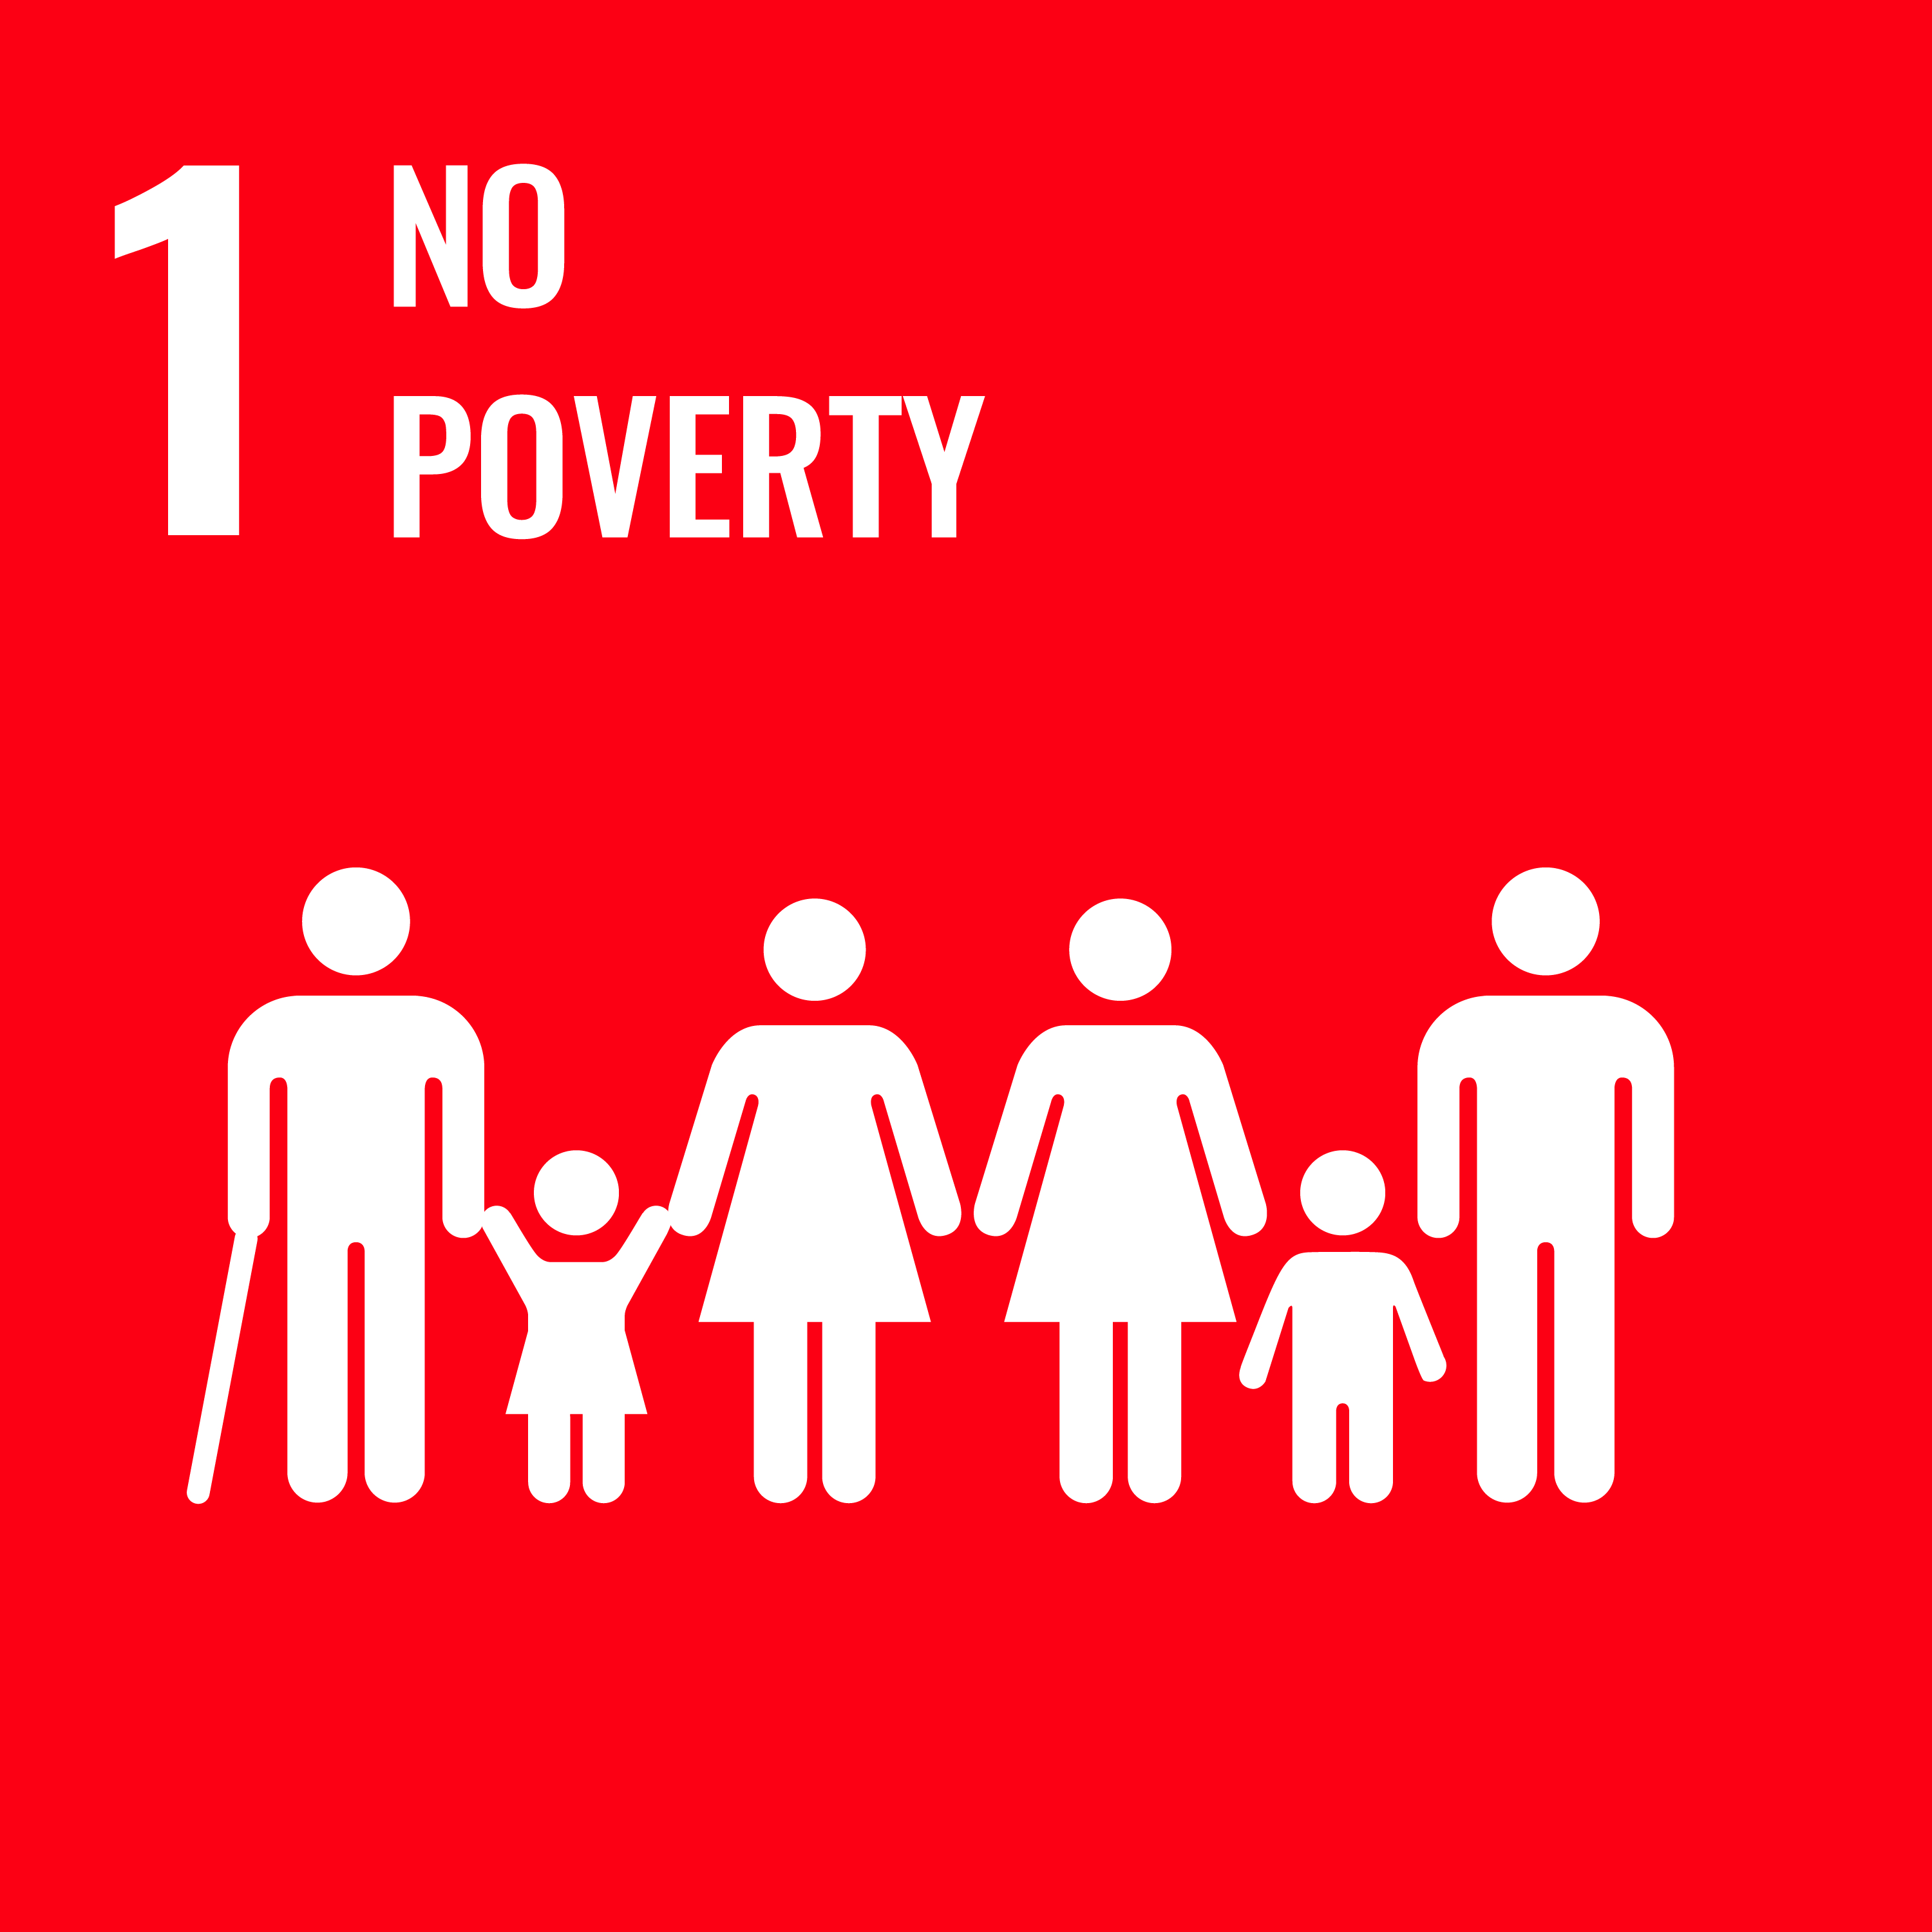
\includegraphics[width=\linewidth]{Pictures/ODD/ODD01.jpg}
%    \end{minipage}
%    \hfill
%    \begin{minipage}{0.8\textwidth}
%        {\bfseries\Large ODD 1 : Pas de pauvreté}\\[2pt]
%        \textit{Éliminer l’extrême pauvreté pour tous d’ici 2030}
%    \end{minipage}
%\end{tcolorbox}
%
%\vspace{0.4cm}
%
%%  Exemple de contenu
%Dans ce cadre, nous analysons la situation du Sénégal par rapport aux cibles :
%\begin{itemize}
%    \item Réduire à 0\% la proportion de population vivant avec moins de 1,90 USD/jour.
%    \item Étendre les systèmes de protection sociale.
%    \item Garantir l’accès universel aux ressources économiques.
%\end{itemize}


\begin{simplebox2}
	
	\begin{minipage}{0.15\textwidth}
		        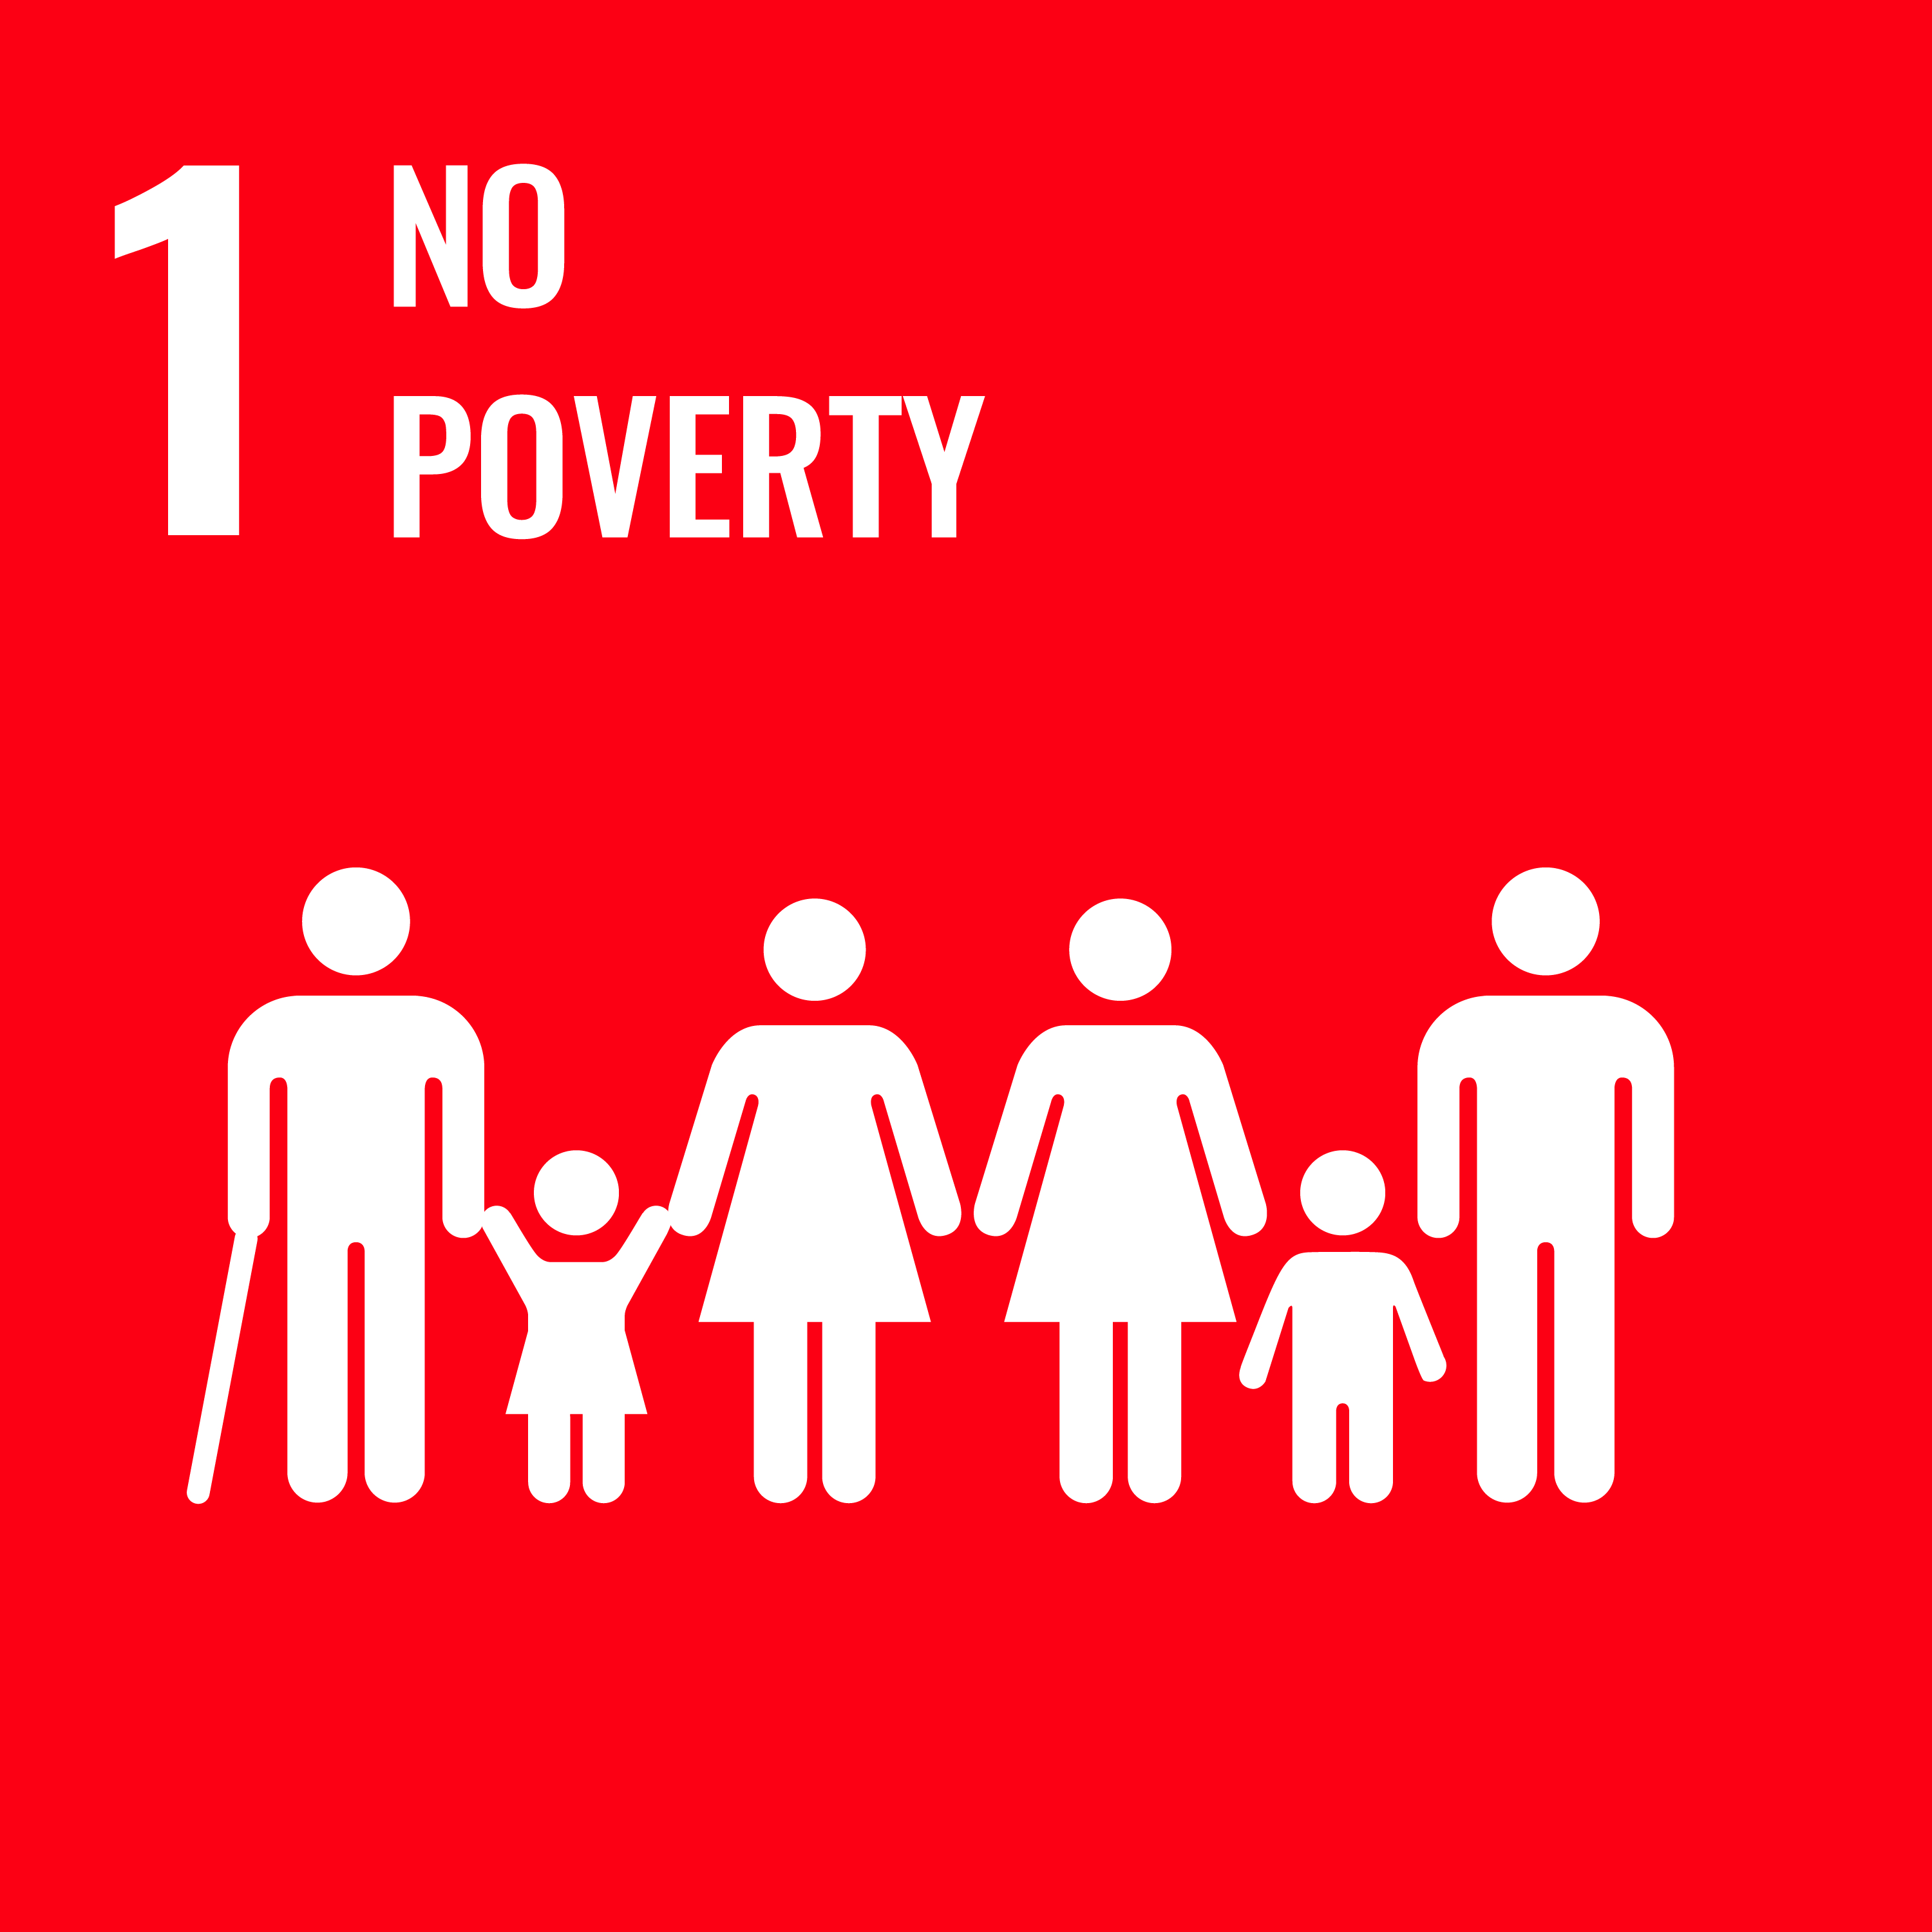
\includegraphics[width=\linewidth]{Pictures/ODD/ODD01.jpg}
		    \end{minipage}
		    \hfill
		    \begin{minipage}{0.8\textwidth}
		        {\bfseries\Large ODD 1 :}\\[2pt]
		        \textit{Éliminer la pauvreté sous toutes ses formes et partout dans le monde}
		    \end{minipage}
\end{simplebox2}

\begin{simplebox}
	Réduire de moitié au moins la proportion d’hommes, de femmes et 
	d’enfants de tous âges souffrant d’une forme ou l’autre de pauvreté, 
	telle que définie par chaque pays.
\end{simplebox}

% ========================
% Section Pauvreté Sénégal
% ========================
\section*{Cible 1.2 : Réduction de la pauvreté}

L’éradication de la pauvreté sous toutes ses formes constitue un des défis majeurs des politiques nationales de développement : le \textbf{Plan Sénégal Émergent (PSE 2014-2018)}, le \textbf{PSE Phase II (2019-2023)} et le \textbf{Plan d’action pour la stabilisation et le développement (PA-SD 2023-2025)}.


Les différents référentiels nationaux ont permis de réduire progressivement la pauvreté. Selon les résultats de l’Enquête harmonisée sur les conditions de vie des ménages (EHCVM) :  

% ------------------------
% Insérer le graphique
% ------------------------
%\begin{figure}[H]
%	\centering
%	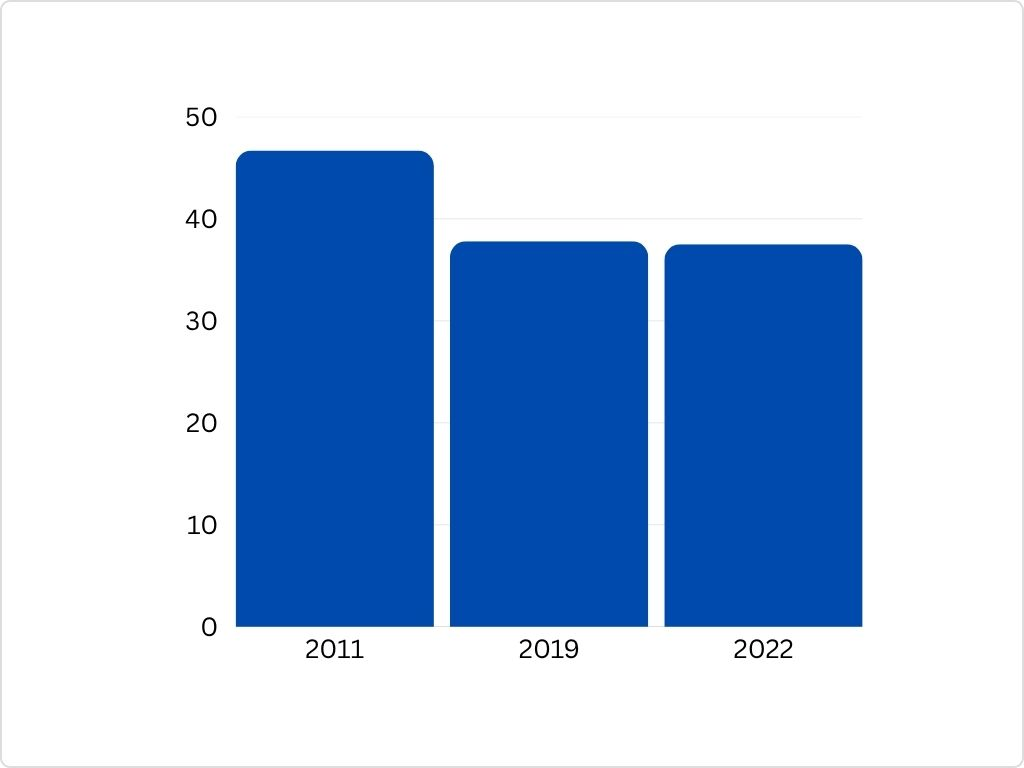
\includegraphics[width=0.9\textwidth]{Pictures/graphe_test.jpg}
%	%\caption{Évolution du taux de pauvreté au Sénégal (EHCVM 2011-2022)}
%\end{figure}


\begin{itemize}
	\item 2011 : incidence de la pauvreté à 46,7\%
	\item 2019 : incidence de la pauvreté à 37,8\%
	\item 2022 : incidence de la pauvreté à 37,5\%
\end{itemize}

L’EHCVM établit une base de référence cohérente pour la mesure et le suivi de la pauvreté. Sur cette base, la population pauvre représente environ 37,5\% de la population nationale, ce qui montre une progression mais indique que la pauvreté reste encore significative au Sénégal.


Le niveau de pauvreté demeure particulièrement marqué dans certaines régions et chez certains ménages. La pauvreté touche plus fortement les ménages ruraux et ceux dirigés par des hommes. L’incidence de la pauvreté monétaire pour les ménages dirigés par des hommes est généralement plus élevée que pour ceux dirigés par des femmes.
\section*{Synthèse de la performance - ODD 1}

Sur la base des indicateurs disponibles, l'évaluation de la performance du Sénégal par rapport aux objectifs de l'ODD 1 produit un \textbf{score global de 67,45\%}, reflétant une situation \textbf{modérément favorable} en matière d'élimination de la pauvreté.

\subsection*{Performance par Indicateur}

\begin{figure}[H]
	\centering
	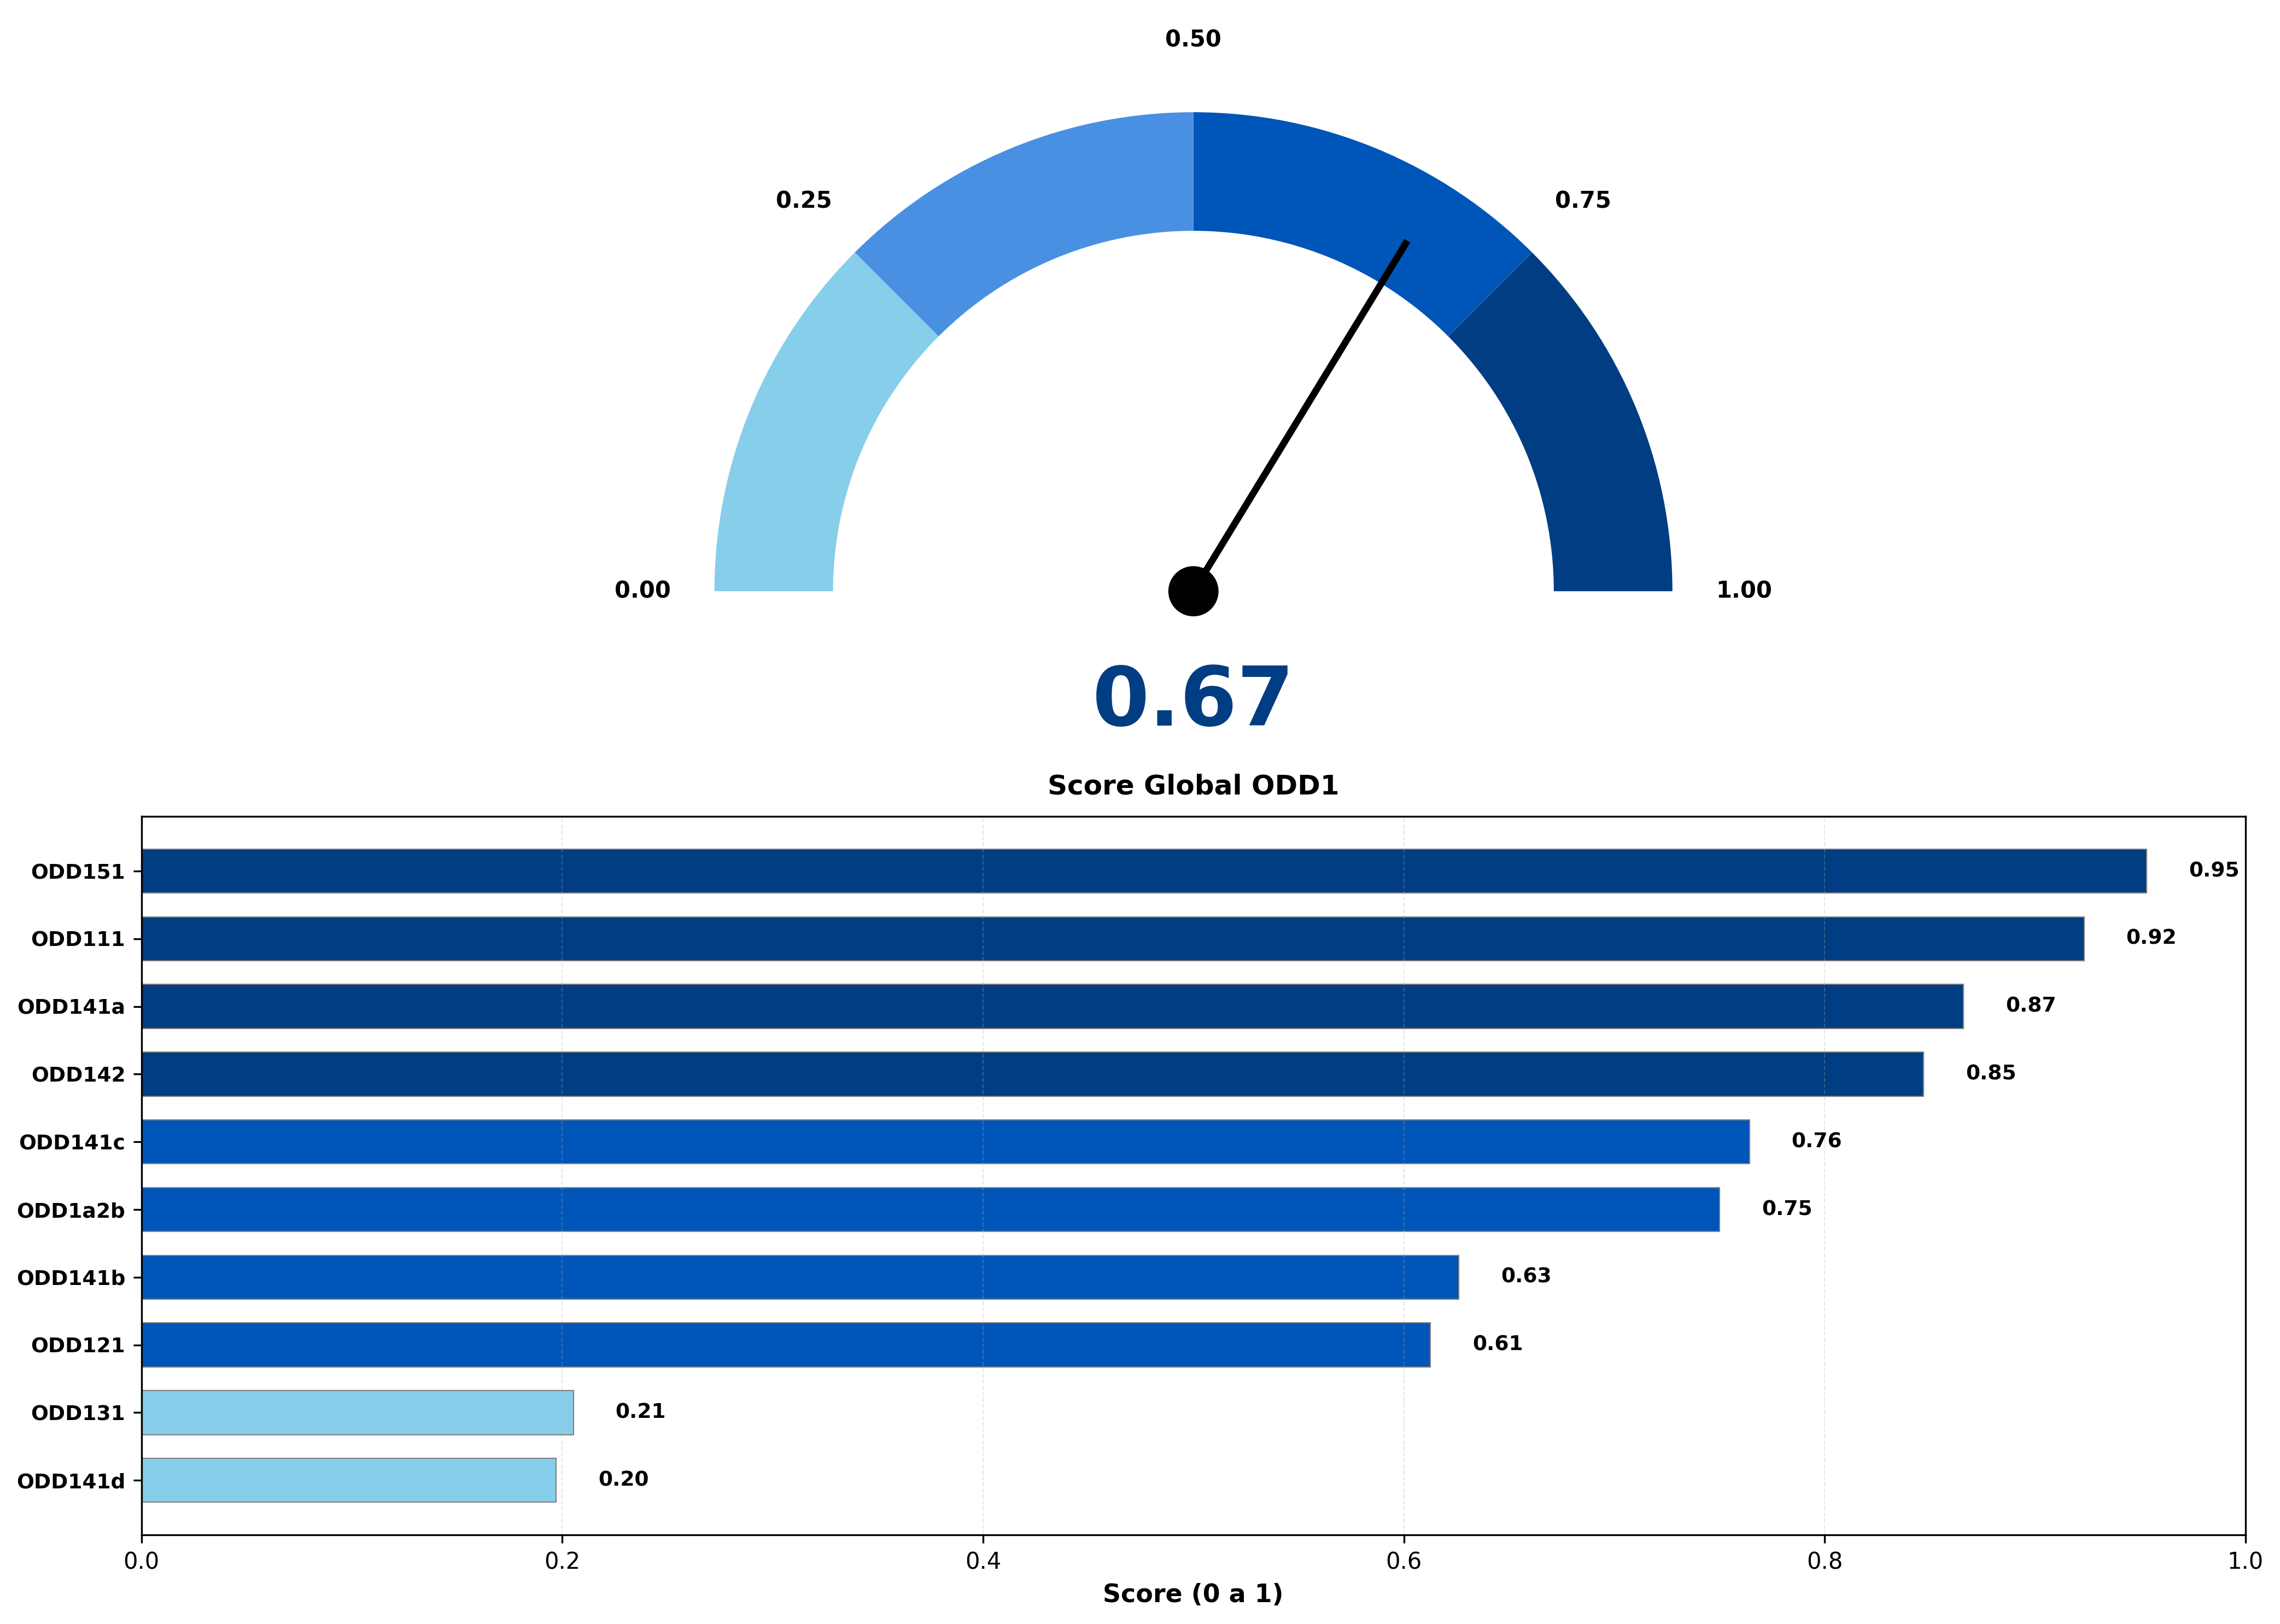
\includegraphics[width=0.95\textwidth]{Pictures/graphs/ODD1_scores.png}
	\caption{Performance par indicateur - ODD 1 (Score global: 67,45\%)}
	\label{fig:odd1_scores}
\end{figure}

\begin{table}[H]
	\caption{Détails des indicateurs - ODD 1}
	\centering
	\small
	\renewcommand{\arraystretch}{1.4}
	\begin{tabularx}{0.85\textwidth}{l l c c c}
		\rowcolor[HTML]{003D82}
		\color{white}\textbf{Code} & \color{white}\textbf{Indicateur} & \color{white}\textbf{Valeur} & \color{white}\textbf{Cible} & \color{white}\textbf{Score} \\
		\rowcolor[HTML]{F5F8FC}
		ODD131 & Protection sociale & 18,48\% & 90,00\% & 0,21 \\
		\rowcolor[HTML]{F5F8FC}
		ODD141d & Énergies/Services basiques & 19,71\% & 100,00\% & 0,20 \\
		\rowcolor[HTML]{E8F0FF}
		ODD121 & Pauvreté nationale & 37,50\% & 18,90\% & 0,61 \\
		\rowcolor[HTML]{E8F0FF}
		ODD141b & Accès ressources (2) & 62,61\% & 100,00\% & 0,63 \\
		\rowcolor[HTML]{F5F8FC}
		ODD1a2 & Investissement éducation & 22,60\% & 30,00\% & 0,75 \\
		\rowcolor[HTML]{F5F8FC}
		ODD141c & Accès ressources (3) & 76,42\% & 100,00\% & 0,76 \\
		\rowcolor[HTML]{E8F0FF}
		ODD142 & Droits économiques & 84,70\% & 100,00\% & 0,85 \\
		\rowcolor[HTML]{E8F0FF}
		ODD141a & Accès ressources (1) & 86,59\% & 100,00\% & 0,87 \\
		\rowcolor[HTML]{F5F8FC}
		ODD111 & Pauvreté extrême & 5,57\% & 0,00\% & 0,92 \\
		\rowcolor[HTML]{F5F8FC}
		ODD151 & Résilience aux désastres & 18,42\% & 14,40\% & 0,95 \\
	\end{tabularx}
	\label{tab:odd1_detailed}
\end{table}

La résilience aux désastres (95,31\%) et la réduction de la pauvreté extrême (92,33\%) affichent des résultats excellents, tandis que l'accès aux droits économiques (84,70\%) et à certaines ressources (76-87\%) progressent favorablement. Cependant, des déficits critiques demeurent: la protection sociale (20,53\%) reste gravement insuffisante, couvrant à peine un cinquième de la population cible, tandis que l'accès à l'électricité et aux services basiques (19,71\%) pose un défi majeur de couverture territoriale, notamment dans les zones rurales. La pauvreté monétaire nationale persiste à 37,50\%, bien au-dessus de la cible 2030 de 18,90\%, exigeant une accélération significative des efforts de réduction. Les quatre priorités stratégiques à court et moyen terme sont: (1) l'universalisation de la protection sociale, aujourd'hui criticalement insuffisante et fondamentale pour atteindre les cibles 2030; (2) l'extension rapide de l'accès à l'électricité et aux services hydrauliques en zones rurales; (3) la consolidation des acquis contre la pauvreté extrême tout en convergant progressivement vers la cible nationale de 18,90\%; et (4) la poursuite de l'investissement public en éducation pour améliorer le capital humain et les opportunités économiques à long terme.















































% =================================================


%\section*{Cible 1.3 : Mettre en place des systèmes et mesures de protection sociale pour tous, adaptés au contexte national}



%La protection sociale constitue un levier central dans la lutte contre la pauvreté. Au Sénégal, malgré plusieurs réformes institutionnelles, les indicateurs produits par l’Agence nationale de la statistique et de la démographie (ANSD) montrent que les progrès restent limités et parfois contradictoires.
%
%Les résultats de l’Enquête Harmonisée sur les Conditions de Vie des Ménages (EHCVM 2018--2019) indiquent que le taux de pauvreté monétaire s’établissait à \textbf{37,8\,\%}, contre 42,8\,\% en 2011, ce qui traduit une amélioration relative du bien-être. Toutefois, en raison de la croissance démographique, le nombre absolu de personnes pauvres est passé de \textbf{5\,832\,008} individus en 2011 à \textbf{6\,032\,379} en 2018, révélant une progression du volume de pauvreté malgré la baisse du taux. Les résultats de l’EHCVM II (2021--2022) confirment cette tendance : bien que le taux de pauvreté décende légèrement à \textbf{37,5\,\%}, l’ANSD estime qu’environ \textbf{500\,000} personnes supplémentaires sont tombées dans la pauvreté durant la période, du fait notamment de la fréquence élevée des chocs socio-économiques.
%
%Selon le rapport final de l’EHCVM II, la vulnérabilité demeure très marquée : \textbf{66,1\,\%} des ménages les plus pauvres déclarent avoir subi au moins un choc au cours des trois années précédant l’enquête. Certaines régions sont particulièrement exposées, comme Diourbel (\textbf{82,4\,\%}), Kaffrine (\textbf{80,5\,\%}) et Saint-Louis (\textbf{80,2\,\%}). Cette exposition accrue fragilise fortement la capacité des ménages à faire face aux aléas et renforce l’importance d’un système de protection sociale efficace.
%
%Sur le plan institutionnel, la Caisse de Sécurité Sociale (CSS) demeure un acteur majeur du dispositif national. Les données du rapport \emph{Situation Économique et Sociale du Sénégal} (SESN 2022--2023) montrent que les charges techniques liées aux prestations familiales atteignent \textbf{15\,105\,925\,904 F CFA} en 2022. Parmi celles-ci, les allocations familiales représentent la plus grande part, avec \textbf{8\,869\,176\,900 F CFA}, soit près de 59\,\% du total. Les allocations de maternité s’élèvent quant à elles à \textbf{696\,796\,200 F CFA}, tandis que les allocations prénatales représentent \textbf{243\,835\,450 F CFA}. Ces montants illustrent l’importance des prestations familiales dans l’architecture de la protection sociale sénégalaise, mais montrent également que d’autres dimensions, telles que l’assurance maladie, restent faiblement développées.
%
%En matière de couverture santé, les données du SESN 2020--2021 indiquent que seuls \textbf{5,2\,\%} des travailleurs bénéficient d’une assurance maladie. Cette proportion atteint \textbf{13,4\,\%} chez les salariés, mais demeure très marginale dans l’emploi non salarié, largement majoritaire au Sénégal. L’informalité persistante limite donc sensiblement la portée des régimes contributifs et constitue l’un des principaux obstacles à l’extension de la protection sociale.
%
%Le Sénégal a néanmoins engagé plusieurs réformes, notamment à travers la Stratégie Nationale de Protection Sociale (SNPS) 2016--2035, qui vise l’extension progressive des filets sociaux, la couverture maladie universelle et la modernisation des mécanismes de soutien aux ménages vulnérables. Cependant, les résultats de l’EHCVM II ainsi que ceux des rapports SESN montrent que les dispositifs restent insuffisamment inclusifs et que leur impact demeure limité face à la fréquence élevée des chocs économiques, climatiques et sanitaires.
%
%


% =================================================


\newpage
\begin{simplebox2}
	
	\begin{minipage}{0.15\textwidth}
		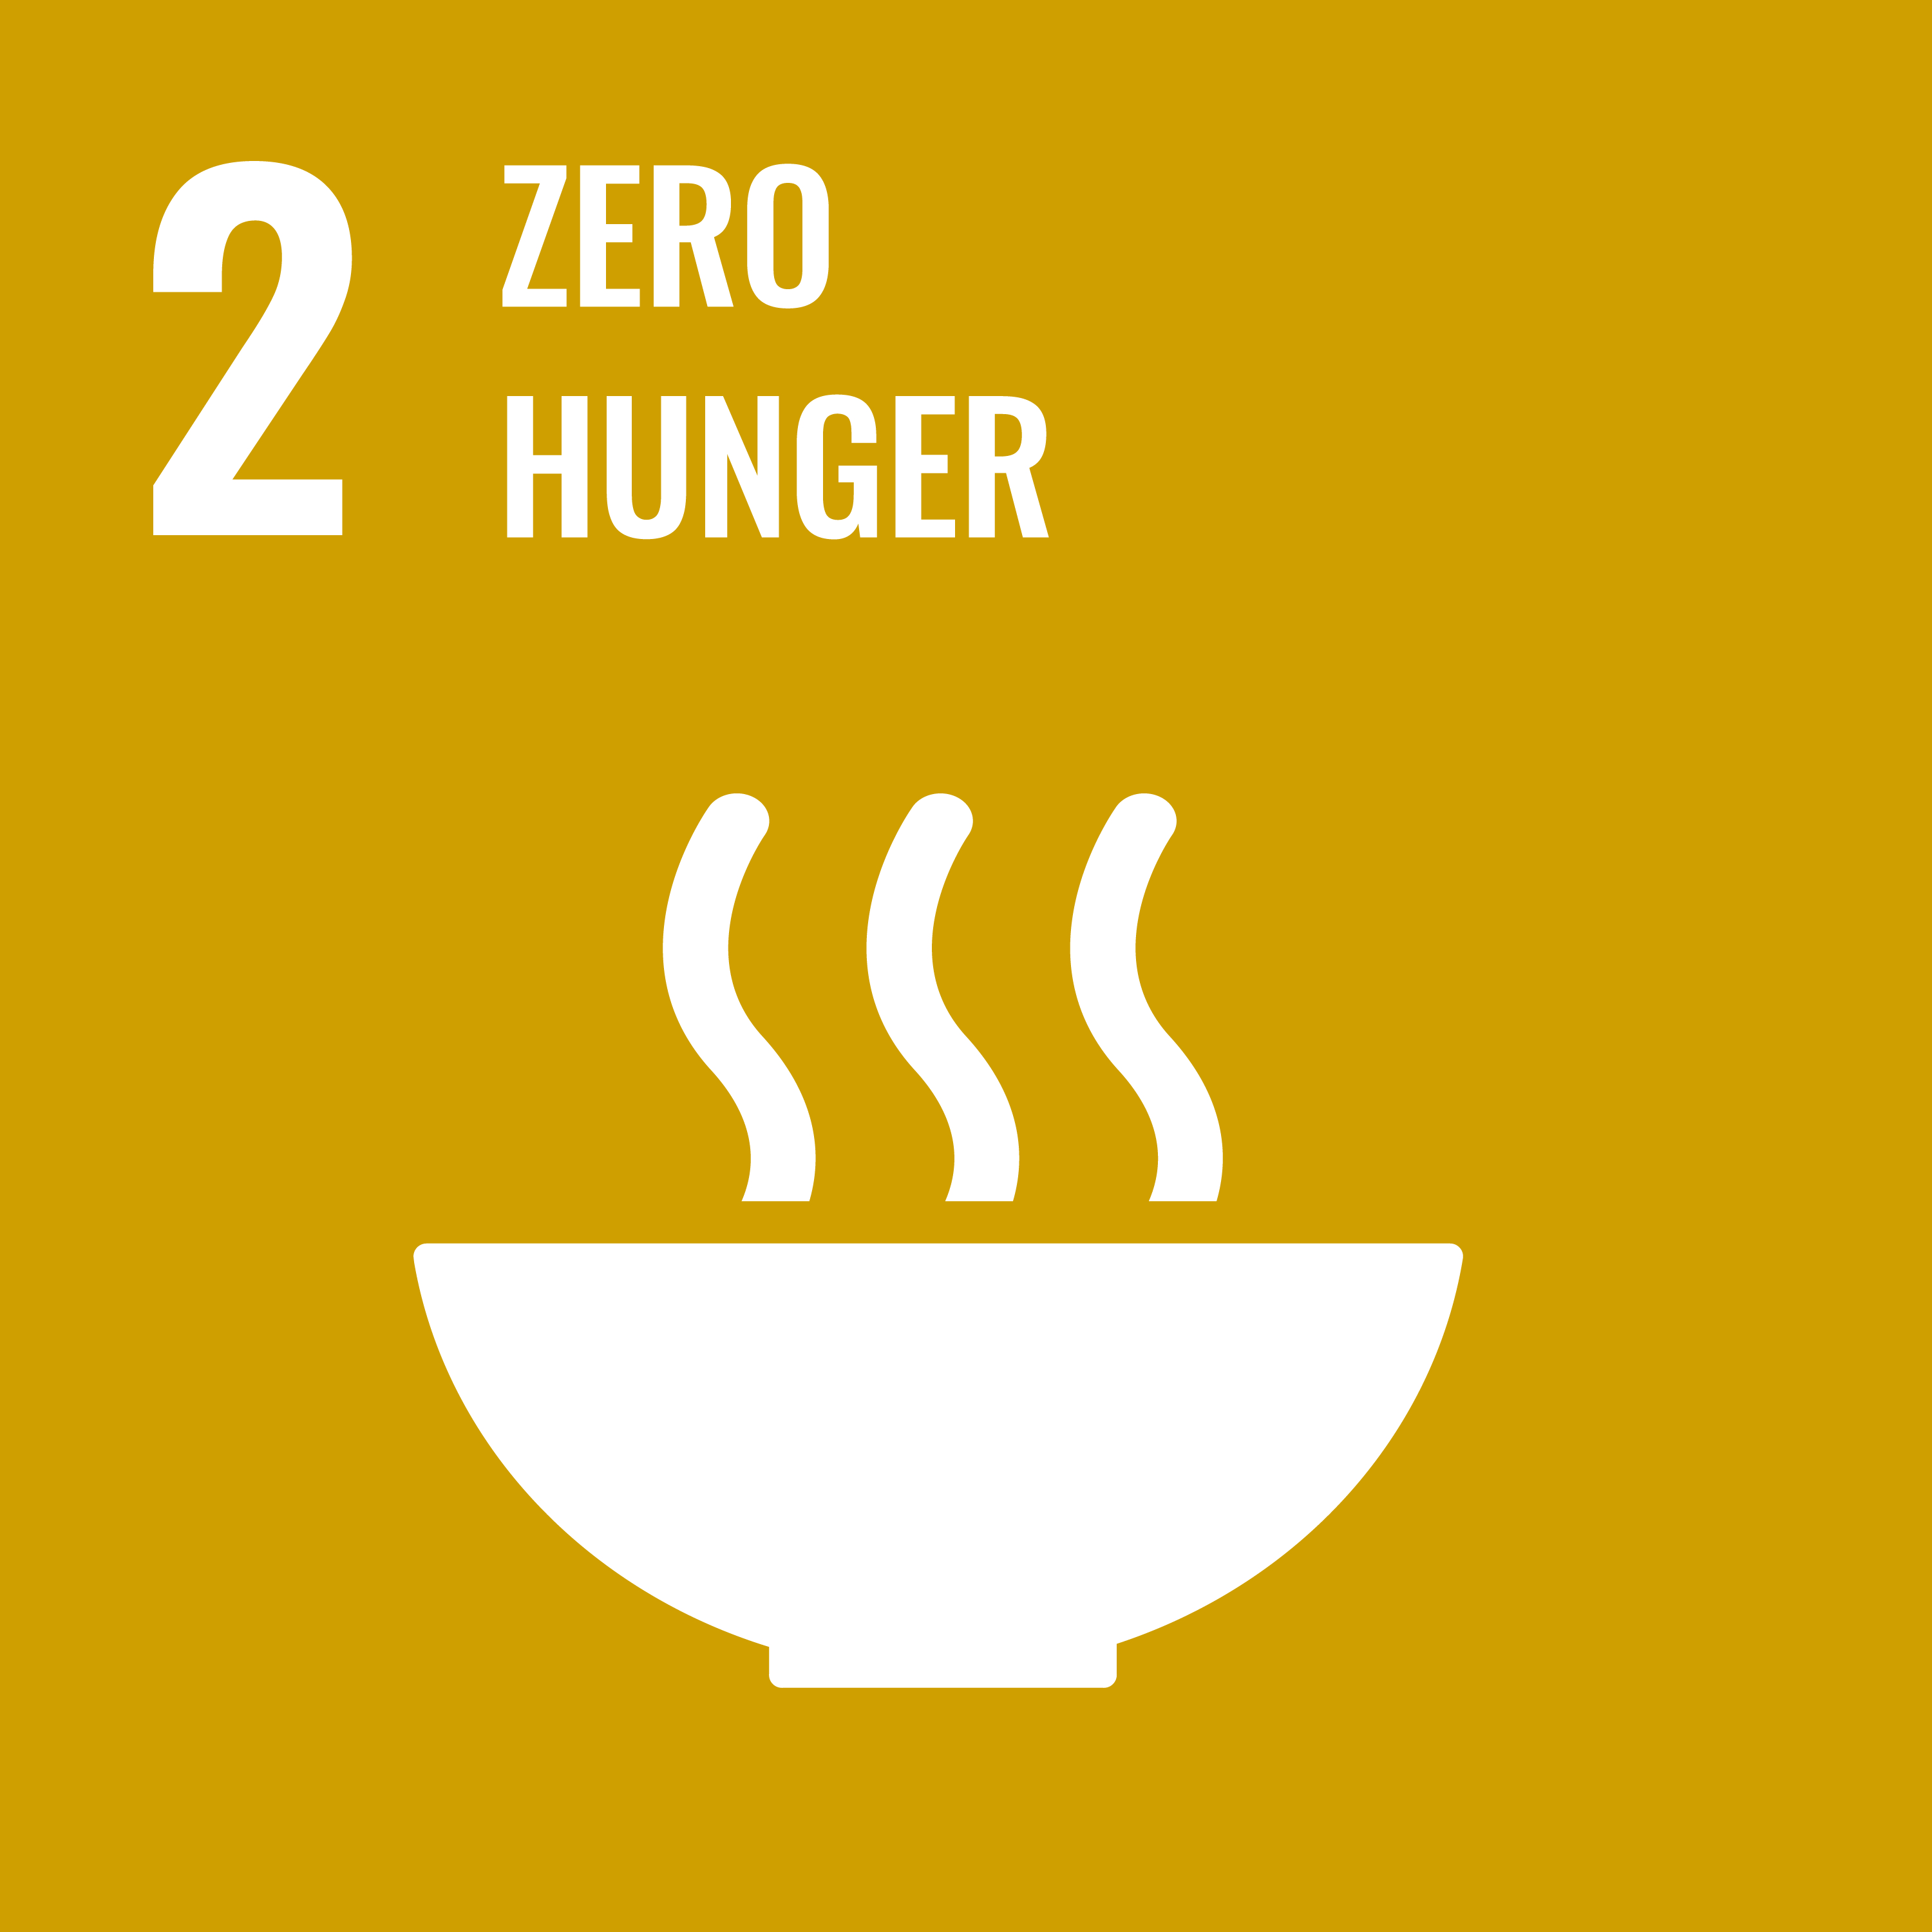
\includegraphics[width=\linewidth]{Pictures/ODD/ODD02.jpg}
	\end{minipage}
	\hfill
	\begin{minipage}{0.8\textwidth}
		{\bfseries\Large ODD 2 : }\\[2pt]
		\textit{ ODD 2 : 
			Éliminer la faim, assurer la sécurité alimentaire, améliorer la nutrition et promouvoir l’agriculture durable}
	\end{minipage}
\end{simplebox2}


\section*{Cible 2.1 : Éliminer la faim d'ici 2030}

La cible 2.1 vise à garantir l’accès de toutes les populations, en particulier les plus vulnérables, à une alimentation saine, nutritive et suffisante tout au long de l’année. Au Sénégal, l’évolution de la sous-alimentation sur la période observée montre une amélioration significative. Le taux de sous-alimentation (\textit{sdg2\_undernsh}) était estimé à environ 26\% au début des années 2000. Celui-ci a suivi une tendance globalement décroissante, passant à 18\%, puis à 13,5\%, avant d’atteindre successivement 11,8\%, 10,7\% et 10,9\% dans la décennie suivante.

Les données les plus récentes indiquent une poursuite du recul, avec des niveaux proches de 5\% au cours des dernières années disponibles, et une valeur minimale observée autour de 4,5–4,7\%. Cette réduction substantielle reflète des progrès importants dans la disponibilité alimentaire, la diversification des sources de revenus des ménages ruraux, le développement de filets sociaux, ainsi que les efforts de résilience face aux chocs climatiques.

Néanmoins, ces avancées restent fragiles. La sécurité alimentaire demeure exposée aux fluctuations de la production agricole, aux hausses des prix internationaux et aux pressions démographiques. Dans ce contexte, atteindre l’élimination totale de la faim d’ici 2030 nécessitera la consolidation des acquis, l'amélioration de la productivité agricole et un renforcement de la protection sociale en direction des ménages les plus vulnérables.

\begin{figure}[h!]
	\centering
	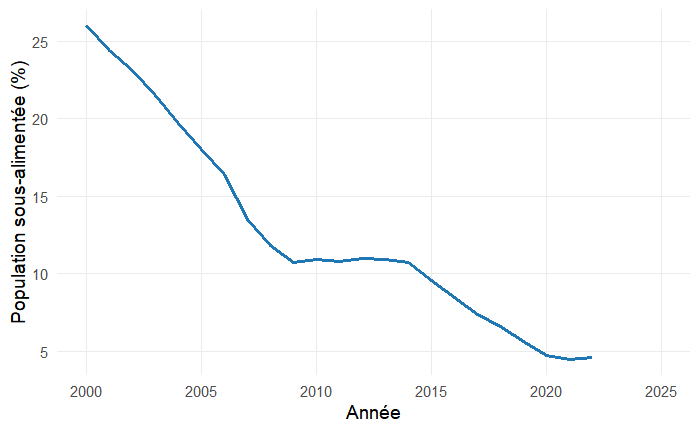
\includegraphics[width=0.9\textwidth]{Pictures/graphs/graph_sous_alimentation.png}
	\caption{Évolution de la sous-alimentation au Sénégal}
\end{figure}





\section*{Cible 2.2 : Mettre fin à toutes les formes de malnutrition}

La cible 2.2 porte sur la réduction des formes de malnutrition touchant principalement les enfants de moins de cinq ans, notamment le retard de croissance et l’émaciation. Au Sénégal, les données issues des indicateurs \textit{sdg2\_stunting} et \textit{sdg2\_wasting} montrent que la situation nutritionnelle s’améliore, mais demeure préoccupante.

Le retard de croissance varie entre 15,5\% et 26,7\% selon les années observées. Les plus fortes valeurs sont enregistrées autour de 26\%, ce qui traduit l'existence de carences nutritionnelles chroniques. Toutefois, une tendance à la baisse semble émerger avec des niveaux autour de 17–18\% puis 15,5\% dans les données les plus récentes. Cette réduction peut s’expliquer par l’amélioration des pratiques de nutrition infantile, l’extension des programmes de supplémentation, ainsi que les actions de dépistage et de prise en charge communautaires.

S’agissant de l’émaciation, les taux oscillent entre 5,9\% et un maximum de 10\%. Malgré une relative stabilité autour de 7–9\%, le pays reste au-dessus du seuil d’alerte de 5\% fixé par l’OMS. Cette persistance de l’émaciation traduit l’impact des crises saisonnières, des déficits alimentaires localisés et des maladies infectieuses qui fragilisent l’état nutritionnel des enfants.

Dans l’ensemble, le Sénégal progresse mais reste éloigné des objectifs internationaux fixés pour 2025. Des efforts supplémentaires seront nécessaires pour réduire durablement la malnutrition, en particulier dans les zones rurales et périurbaines.

\begin{figure}[h!]
	\centering
	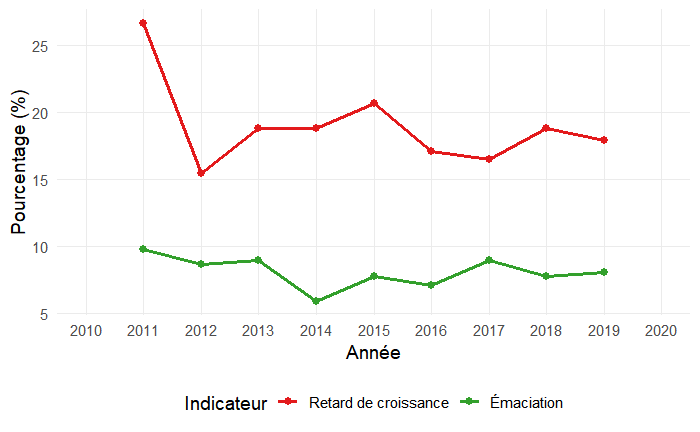
\includegraphics[width=0.9\textwidth]{Pictures/graphs/graph_malnutrition.png}
	\caption{Tendances du retard de croissance et de l'émaciation chez les enfants de moins de 5 ans}
\end{figure}


\section*{Synthèse de la performance - ODD2}

\begin{figure}[H]
	\centering
	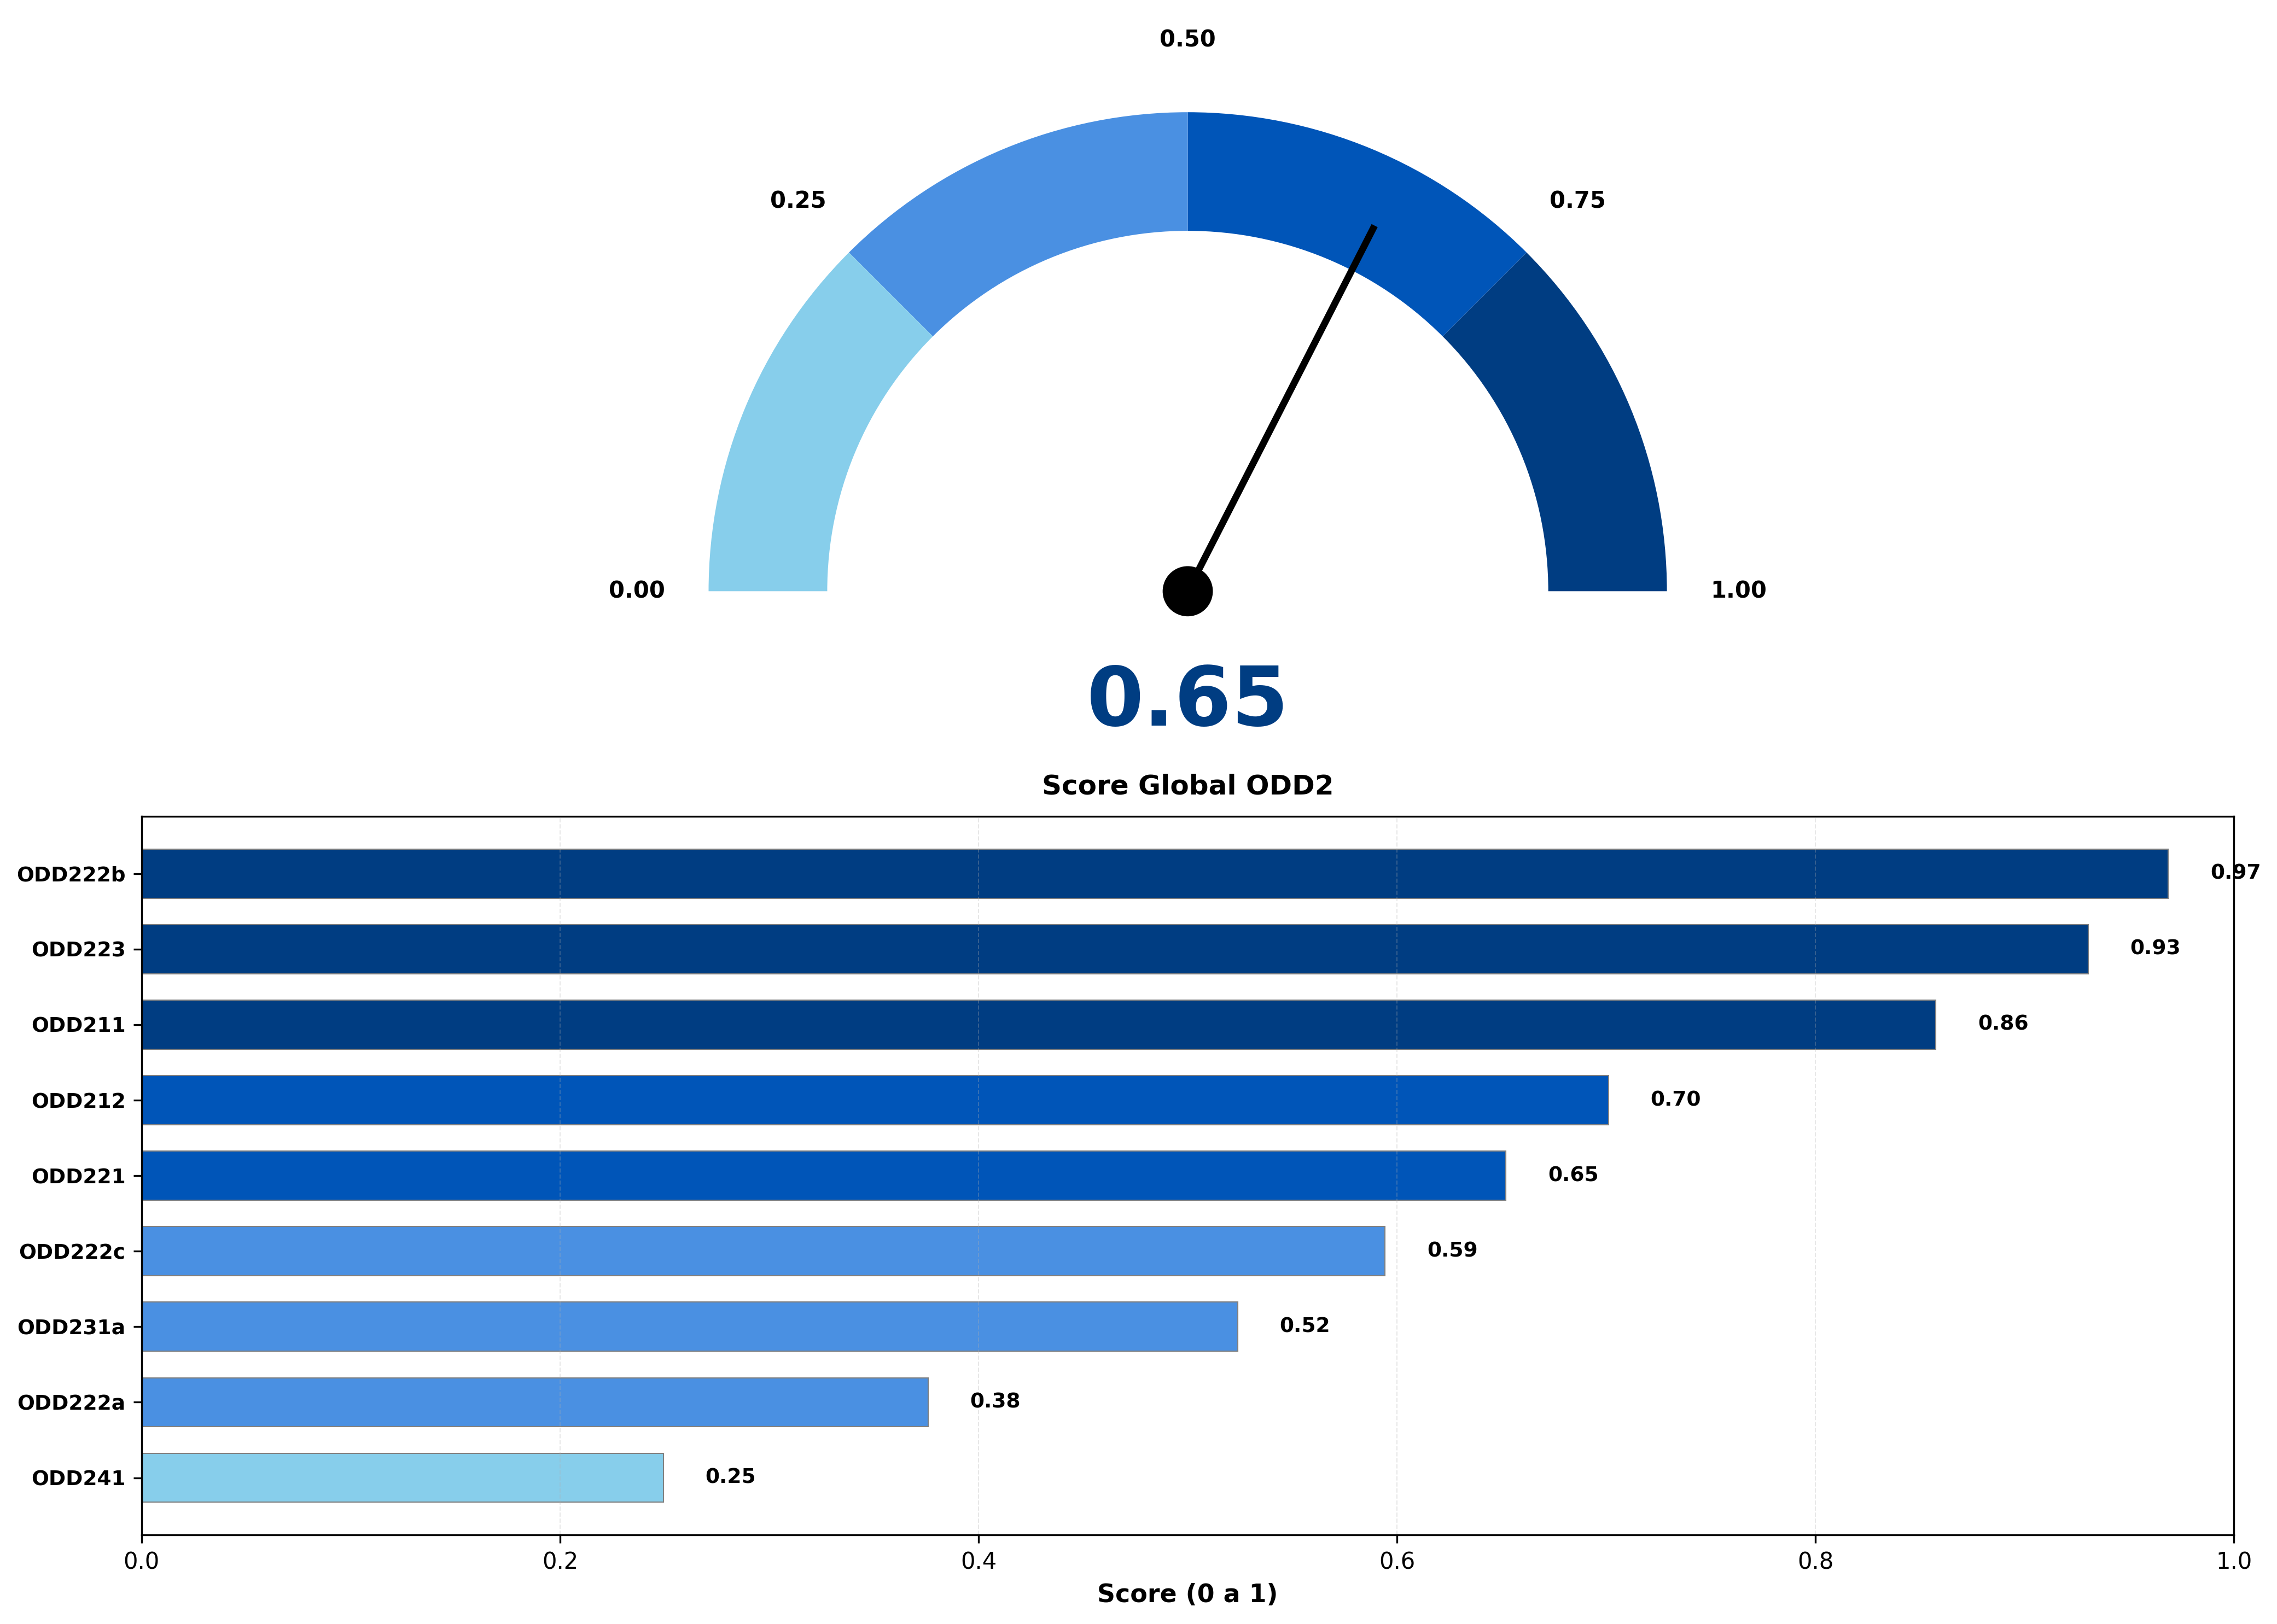
\includegraphics[width=0.95\textwidth]{Pictures/graphs/ODD2_scores.png}
	\caption{Performance par indicateur - ODD2}
\end{figure}

\begin{table}[H]
	\centering
	\begin{tabularx}{\textwidth}{l l c c c}
		\rowcolor[HTML]{003D82}
		\color{white}\textbf{Code} & \color{white}\textbf{Indicateur} & \color{white}\textbf{Valeur} & \color{white}\textbf{Cible} & \color{white}\textbf{Score} \\
		\rowcolor[HTML]{F5F8FC}
		ODD241 & Proportion des zones agricoles exploitées & 0.14 & 0.55 & 0.25 \\
		\rowcolor[HTML]{E8F0FF}
		ODD222a & Emaciation parmi les enfants de moins de 5 ans & 0.10 & 0.00 & 0.38 \\
		\rowcolor[HTML]{F5F8FC}
		ODD231a & Volume de production par unité de travail & 2430.00 & 4638.67 & 0.52 \\
		\rowcolor[HTML]{E8F0FF}
		ODD222c & Insuffisance pondérale parmi les enfants de moins de 5 ans & 0.16 & 0.00 & 0.59 \\
		\rowcolor[HTML]{F5F8FC}
		ODD221 & Retard de croissance parmi les enfants de moins de 5 ans & 0.17 & 0.00 & 0.65 \\
		\rowcolor[HTML]{E8F0FF}
		ODD212 & Prévalence de l'insécurité alimentaire & 0.30 & 0.00 & 0.70 \\
		\rowcolor[HTML]{F5F8FC}
		ODD211 & Prévalence de la sous-alimentation & 0.06 & 0.00 & 0.86 \\
		\rowcolor[HTML]{E8F0FF}
		ODD223 & Anémie chez les femmes âgées de 15 à 49 ans & 0.07 & 0.00 & 0.93 \\
		\rowcolor[HTML]{F5F8FC}
		ODD222b & Surpoids (obésité) parmi les enfants de moins de 5 ans & 0.01 & 0.00 & 0.97 \\
	\end{tabularx}
\end{table}

L'analyse du ODD2 révèle un score global de 0.6504, basé sur 9 indicateur(s). Les performances varient de 0.25 à 0.97, montrant une certaine disparité dans la mise en oeuvre des cibles. Les indicateurs critiques (score < 0,30) nécessitent une attention particulière.



% ========================   OOD 3  ======================================




\newpage
\begin{simplebox2}
	
	\begin{minipage}{0.15\textwidth}
		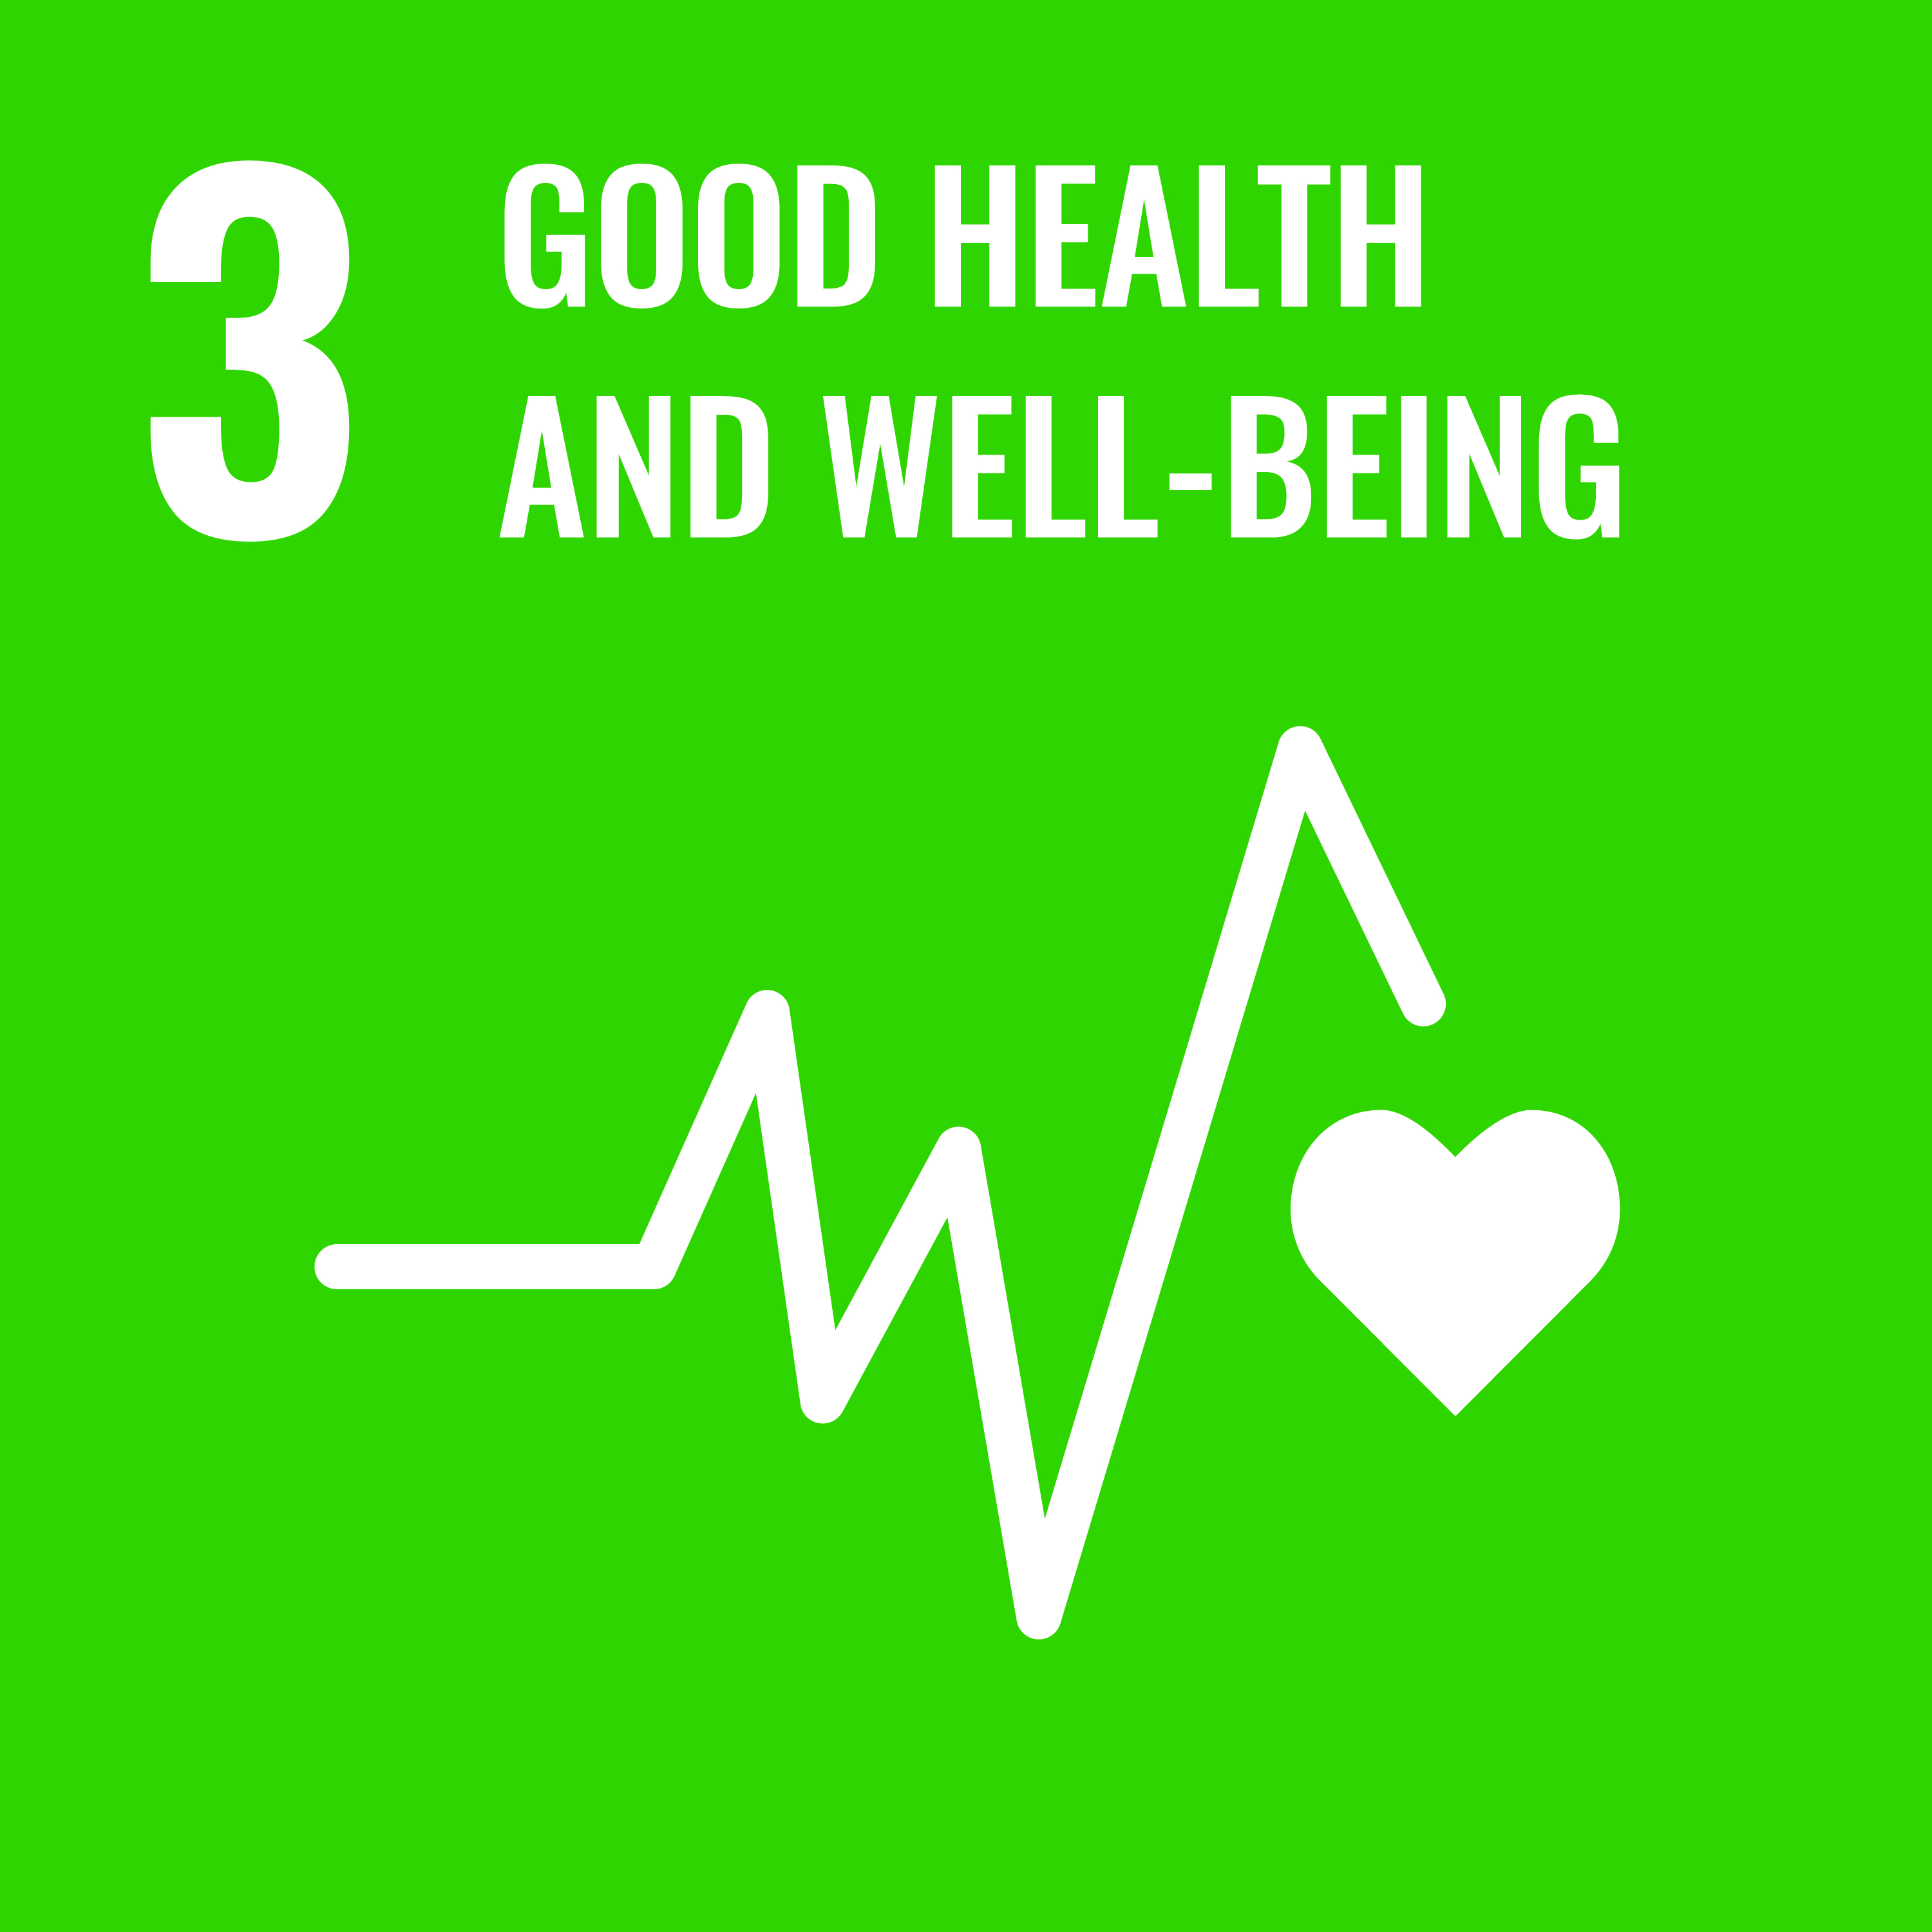
\includegraphics[width=\linewidth]{Pictures/ODD/ODD03.jpg}
	\end{minipage}
	\hfill
	\begin{minipage}{0.8\textwidth}
		{\bfseries\Large ODD 3 : }\\[2pt]
		\textit{
		Permettre à tous de vivre  
		en bonne santé et promouvoir  
		le bien-être de tous à tout âge}
	\end{minipage}
\end{simplebox2}

\section*{Cible 3.1 : Réduire la mortalité maternelle}

La mortalité maternelle est le nombre de femmes, âgées de 15 à 49 ans, décédant pour des causes liées à la grossesse ou à l'accouchement, pour 100 000 naissances vivantes. Entre 2000 et 2025, on observe une diminution progressive du taux, passant de 581 décès pour 100 000 naissances en 2000 à environ 252 décès en 2020. Cette baisse reflète l'amélioration des services de santé maternelle, de la formation du personnel médical et des programmes de santé publique ciblés.

\begin{figure}[H]
	\centering
	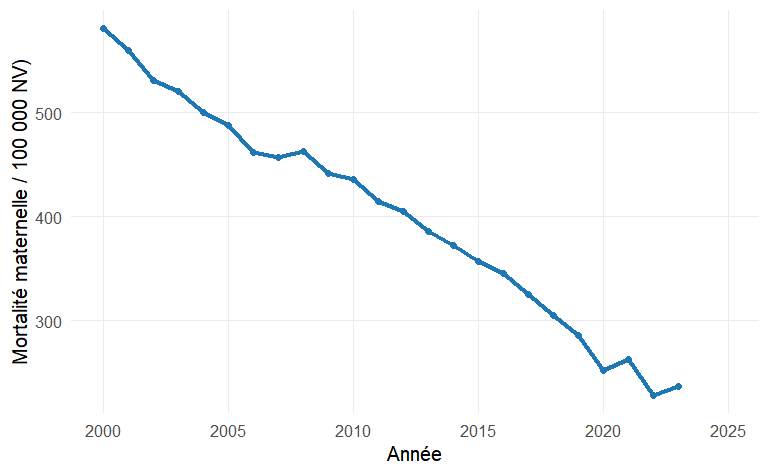
\includegraphics[width=0.8\textwidth]{Pictures/graphs/matmort.png}
	\caption{Évolution de la mortalité maternelle }
\end{figure}

Malgré cette tendance, le taux reste encore au-dessus de l'objectif de 70 décès par 100 000 naissances fixé pour 2030, indiquant un besoin continu d'interventions et d'investissements dans le secteur de la santé maternelle.




\section*{Cible 3.2 : Réduire la mortalité néonatale et infantile}

Le taux de mortalité néonatale représente le nombre de nouveau-nés mourant avant 28 jours, pour 1 000 naissances vivantes, tandis que la mortalité des enfants de moins de 5 ans représente le nombre d'enfants décédant avant cet âge pour 1 000 naissances. Entre 2010 et 2020, la mortalité néonatale est passée de 27,72 à 26,16 pour 1 000, et la mortalité <5 ans de 66,32 à 46,46 pour 1 000 naissances.

\begin{figure}[H]
	\centering
	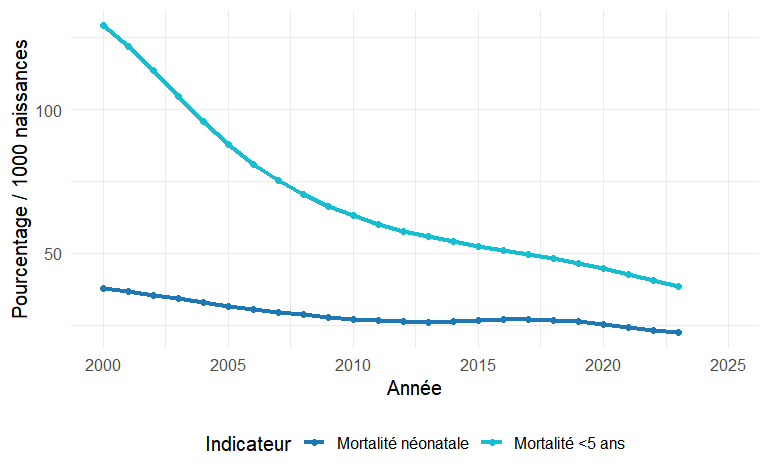
\includegraphics[width=0.8\textwidth]{Pictures/graphs/mortality.png}
	\caption{Évolution de la mortalité néonatale et infantile}
\end{figure}

Cette tendance montre des progrès significatifs grâce à la vaccination, l'amélioration de l'accès aux soins néonataux et la nutrition infantile. Cependant, les taux restent supérieurs aux objectifs de 12 et 25 pour 2030, nécessitant des efforts supplémentaires.



\section*{Cible 3.3 : Lutter contre les maladies transmissibles et non transmissibles}

L'incidence de la tuberculose (TB) est mesurée par le nombre de nouveaux cas pour 100 000 habitants. Le taux de nouvelles infections au VIH correspond au nombre d'individus nouvellement infectés par 1 000 personnes non infectées, et le taux de mortalité lié aux maladies non transmissibles (NCDs) est exprimé en pourcentage d'adultes de 30 à 70 ans décédant de maladies cardiovasculaires, de cancers, de diabète ou d’affections respiratoires chroniques.

Sur la période 2000 - 2025, les trois indicateurs présentent des évolutions contrastées. L’incidence de la tuberculose diminue progressivement, passant d’environ 155 nouveaux cas pour 100\,000 habitants en 2000 à près de 110 cas au milieu des années 2020. Cette tendance traduit les efforts en matière de dépistage, de prise en charge thérapeutique et d’amélioration du suivi communautaire. La baisse reste toutefois modérée, ce qui montre que la tuberculose demeure une maladie persistante nécessitant une surveillance renforcée.

Les nouvelles infections au VIH connaissent une réduction beaucoup plus marquée. Le taux chute de 0{,}63 pour 1\,000 personnes non infectées au début des années 2000 à environ 0{,}10 vingt ans plus tard. Cette évolution témoigne de l’efficacité des campagnes de prévention, notamment la promotion du dépistage précoce, l’accès au traitement antirétroviral et la diminution des transmissions mère-enfant. Cette réduction rapide constitue l’un des progrès les plus significatifs observés parmi les maladies transmissibles.

La mortalité liée aux maladies non transmissibles suit une dynamique différente. Le taux passe de 24{,}5\,\% en 2000 à environ 22{,}3\,\% à l’horizon 2020, révélant une diminution légère mais régulière. Cette évolution souligne l’importance croissante des politiques de prévention, en particulier la lutte contre les facteurs de risque tels que l’hypertension, le diabète, la mauvaise alimentation ou le tabagisme. Toutefois, la réduction demeure limitée, rappelant que les maladies non transmissibles constituent aujourd’hui la principale charge sanitaire structurelle dans la région.


\begin{figure}[H]
	\centering
	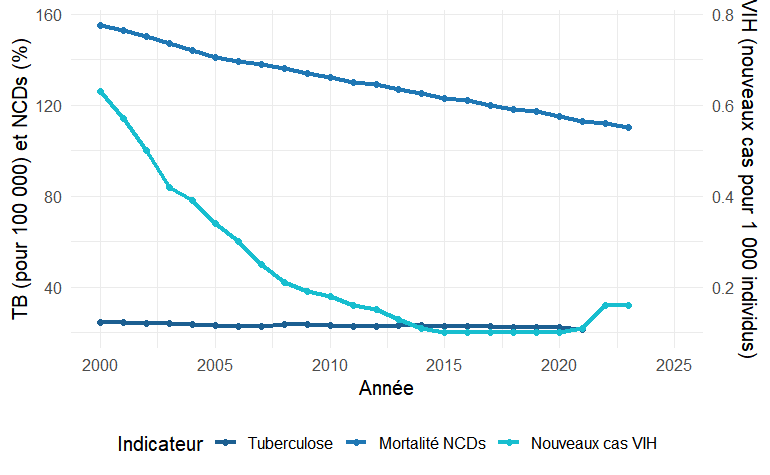
\includegraphics[width=0.8\textwidth]{Pictures/graphs/diseases.png}
	\caption{Évolution des maladies transmissibles et non transmissibles (2000-2025) avec unités distinctes}
\end{figure}



\section*{Synthèse de la performance - ODD3}

\begin{figure}[H]
	\centering
	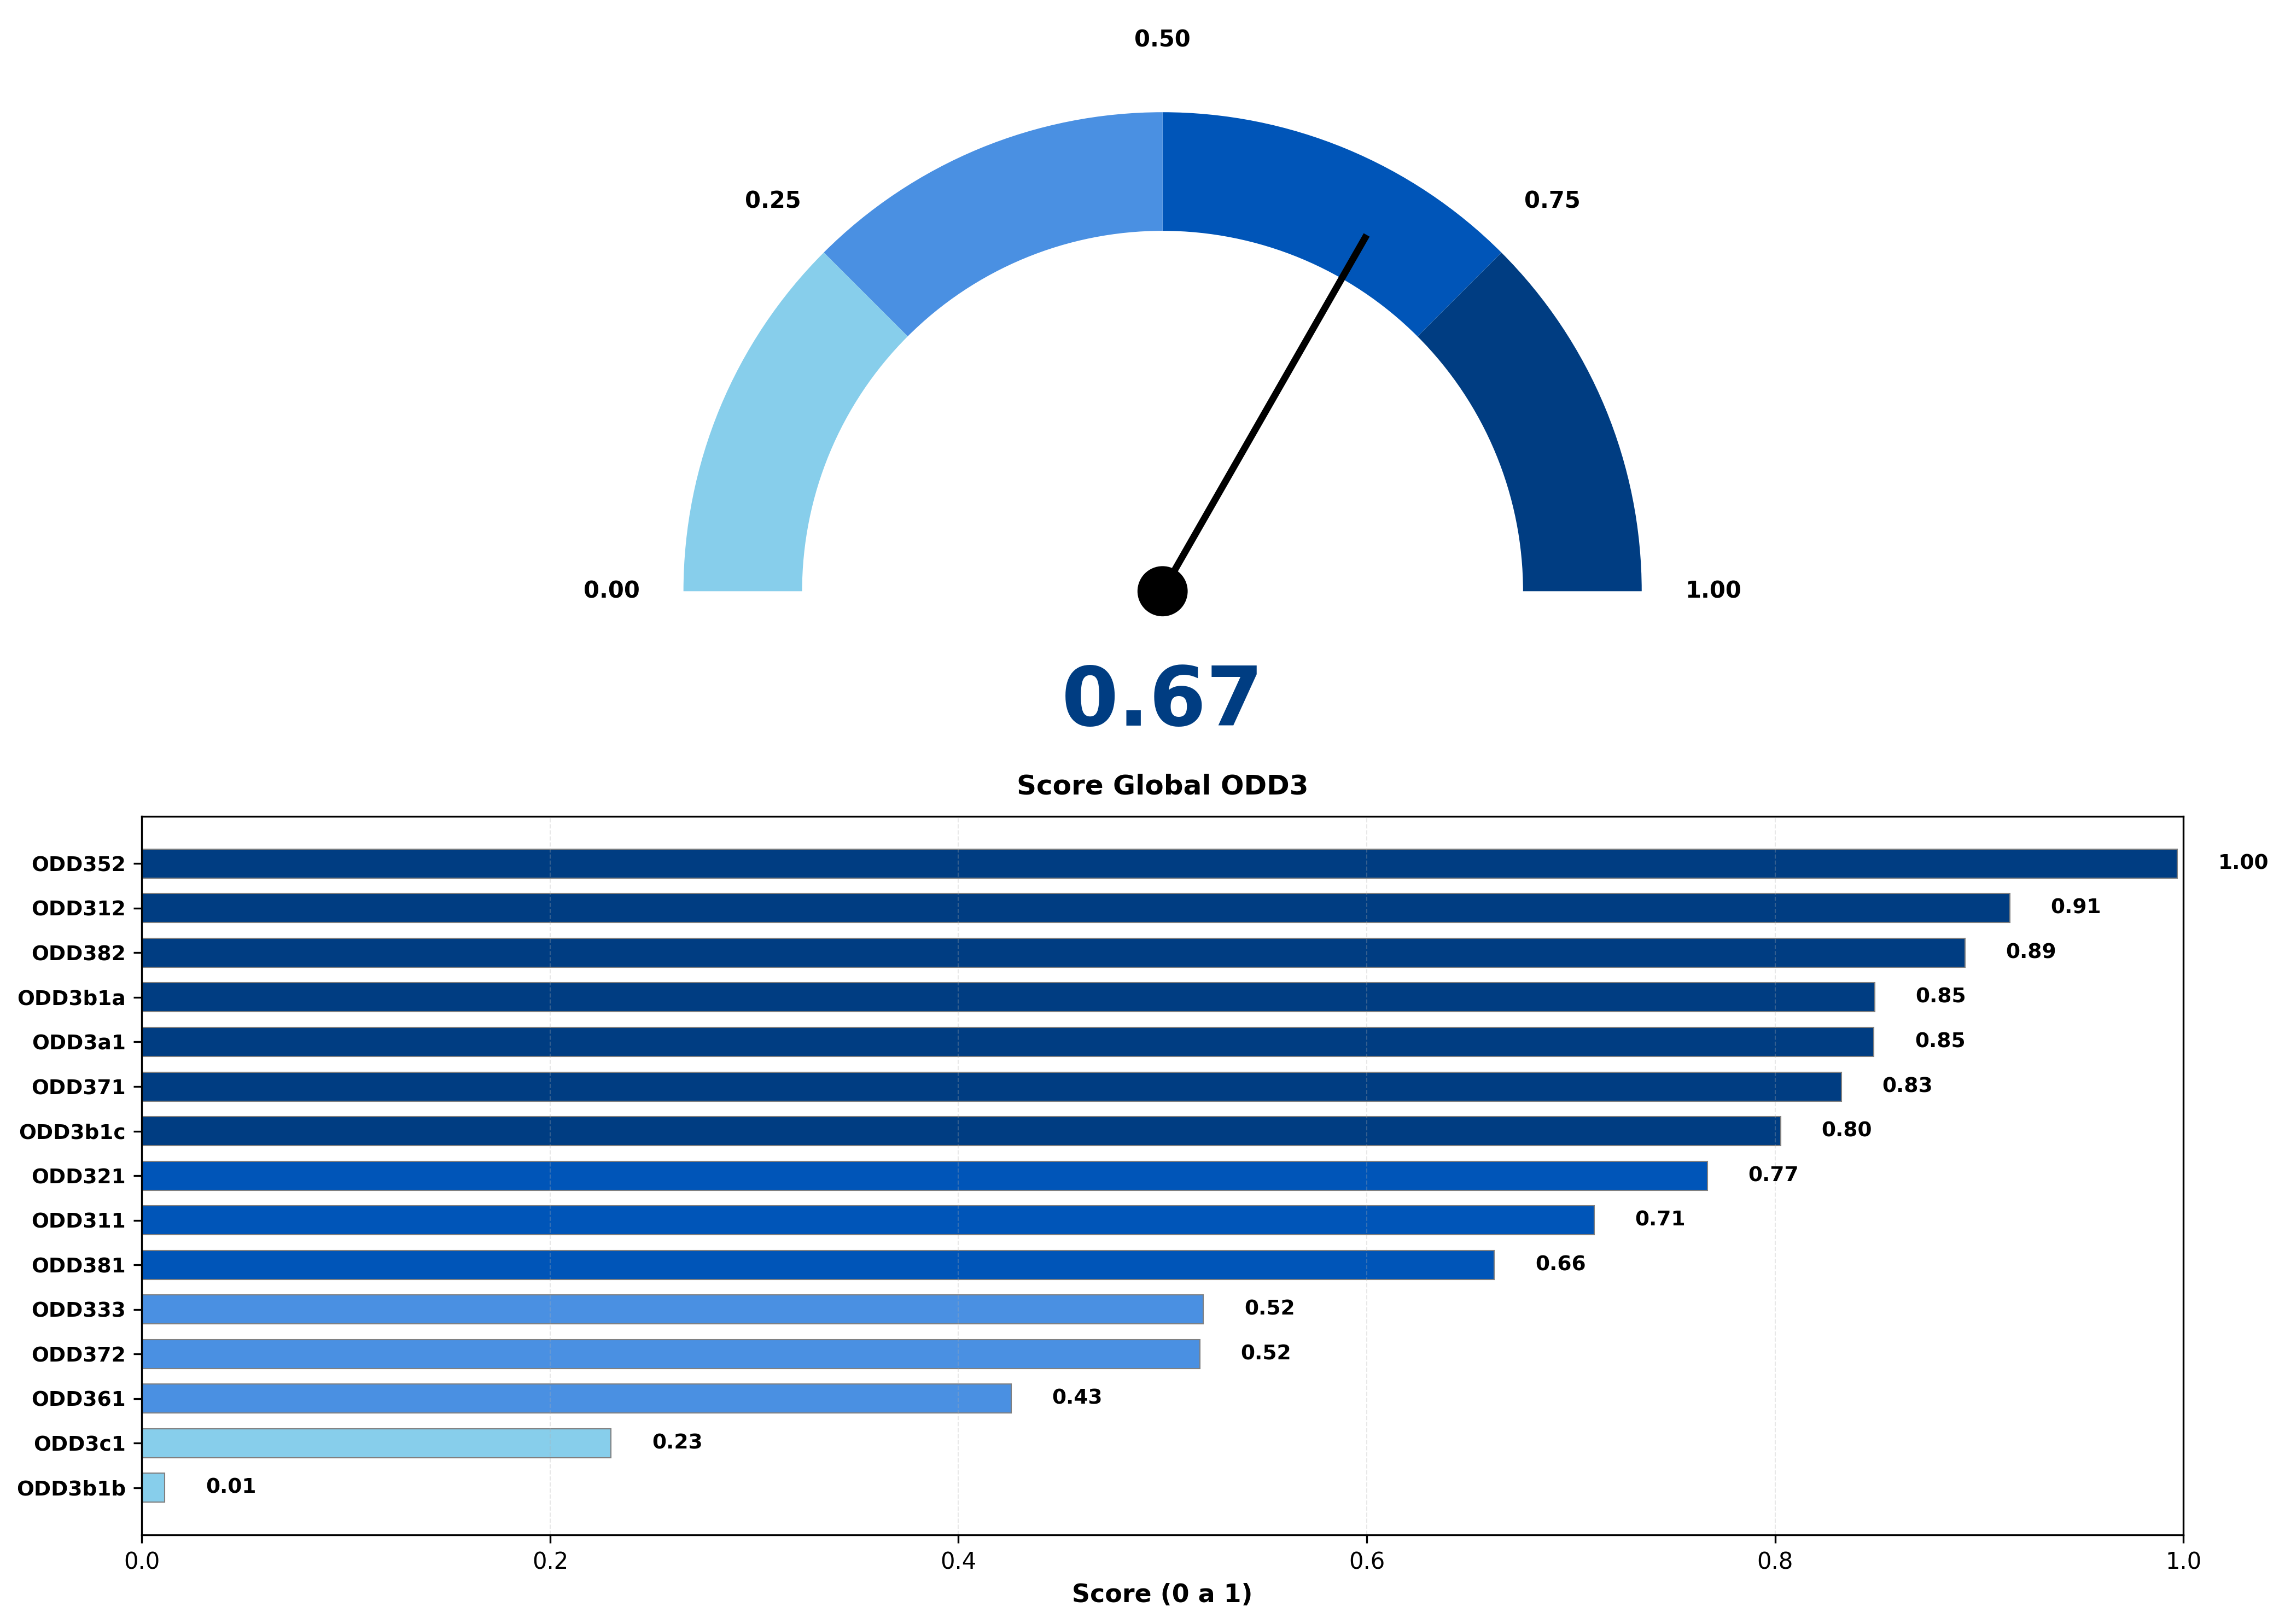
\includegraphics[width=0.95\textwidth]{Pictures/graphs/ODD3_scores.png}
	\caption{Performance par indicateur - ODD3}
\end{figure}

\begin{table}[H]
	\centering
	\begin{tabularx}{\textwidth}{l l c c c}
		\rowcolor[HTML]{003D82}
		\color{white}\textbf{Code} & \color{white}\textbf{Indicateur} & \color{white}\textbf{Valeur} & \color{white}\textbf{Cible} & \color{white}\textbf{Score} \\
		\rowcolor[HTML]{F5F8FC}
		ODD3b1b & Couverture du vaccin contre la rougeole (2nd dose) & 0.42 & 0.90 & 0.01 \\
		\rowcolor[HTML]{E8F0FF}
		ODD3c1 & Densité et répartition du personnel de santé & 1.10 & 4.45 & 0.23 \\
		\rowcolor[HTML]{F5F8FC}
		ODD361 & Mortalité liée aux accidents de la route & 20.80 & 3.00 & 0.43 \\
		\rowcolor[HTML]{E8F0FF}
		ODD372 & Taux de natalité chez les adolescentes & 69.00 & 3.00 & 0.52 \\
		\rowcolor[HTML]{F5F8FC}
		ODD333 & Taux de prévalence du paludisme & 48.00 & 0.00 & 0.52 \\
		\rowcolor[HTML]{E8F0FF}
		ODD381 & Couverture des services de santé essentiels & 53.00 & 80.00 & 0.66 \\
		\rowcolor[HTML]{F5F8FC}
		ODD311 & Taux de mortalité maternelle (pour 100 000 naissances) & 237.00 & 3.00 & 0.71 \\
		\rowcolor[HTML]{E8F0FF}
		ODD321 & Taux de mortalité  infanto-juvénile  (pour 1000) & 65.80 & 25.00 & 0.77 \\
		\rowcolor[HTML]{F5F8FC}
		ODD3b1c & Couverture du vaccin contre le pneumocoque & 0.80 & 0.90 & 0.80 \\
		\rowcolor[HTML]{E8F0FF}
		ODD371 & Besoins satisfaits en matière de planification fa & 0.57 & 0.48 & 0.83 \\
		\rowcolor[HTML]{F5F8FC}
		ODD3a1 & Utilisation actuelle de tabac parmi les personnes & 0.10 & 0.04 & 0.85 \\
		\rowcolor[HTML]{E8F0FF}
		ODD3b1a & Couverture du vaccin DTC (3e dose) & 0.83 & 0.90 & 0.85 \\
		\rowcolor[HTML]{F5F8FC}
		ODD382 & Grandes part des dépenses en santé & 0.07 & 0.04 & 0.89 \\
		\rowcolor[HTML]{E8F0FF}
		ODD312 & Assistance des accouchements par un prestataire qu & 0.93 & 1.00 & 0.91 \\
		\rowcolor[HTML]{F5F8FC}
		ODD352 & Consommation d'alcool pur (en litres) par habitant & 0.04 & 0.00 & 1.00 \\
	\end{tabularx}
\end{table}

L'analyse du ODD3 révèle un score global de 0.6656, basé sur 15 indicateur(s). Les performances varient de 0.01 à 1.00, montrant une certaine disparité dans la mise en oeuvre des cibles. Les indicateurs critiques (score < 0,30) nécessitent une attention particulière.



\newpage
\begin{simplebox2}
	
	\begin{minipage}{0.15\textwidth}
		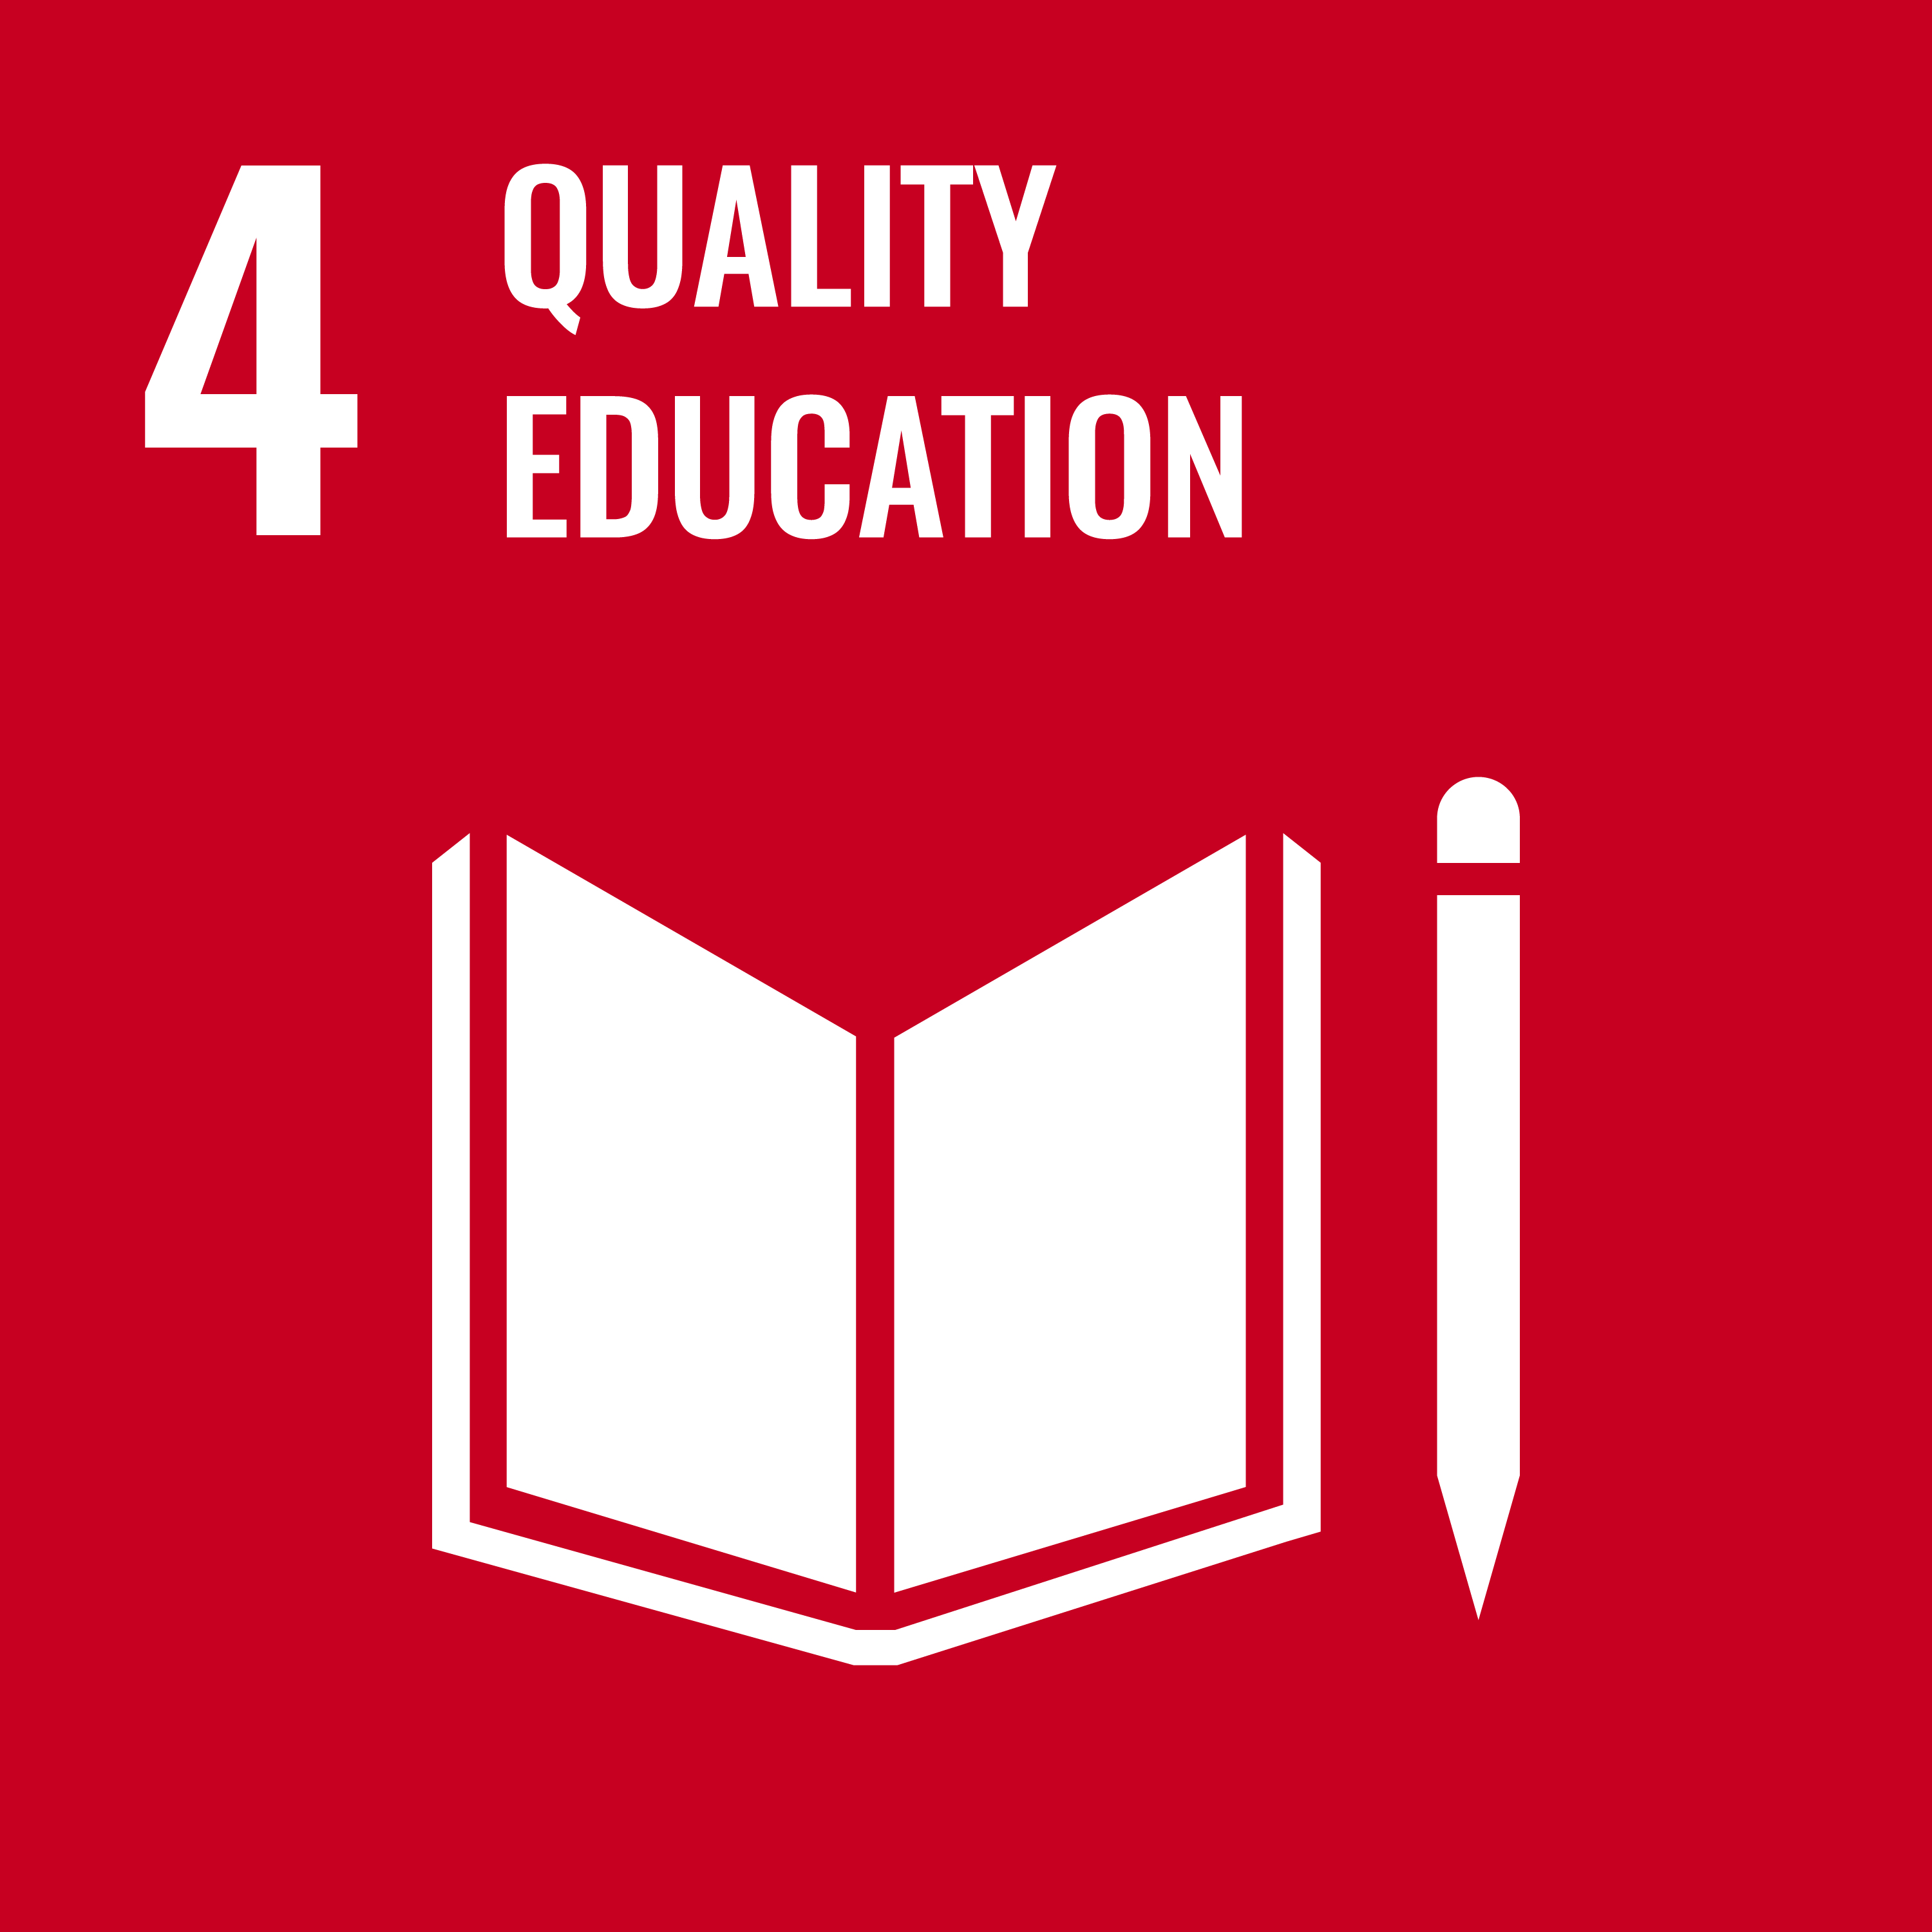
\includegraphics[width=\linewidth]{Pictures/ODD/ODD04.jpg}
	\end{minipage}
	\hfill
	\begin{minipage}{0.8\textwidth}
		{\bfseries\Large ODD 4 : }\\[2pt]
		\textit{ Assurer à tous une éducation équitable, inclusive et de qualité et des possibilités d’apprentissage tout au long de la vie}
	\end{minipage}
\end{simplebox2}






\section*{Cible 4.1 : Enseignement primaire et secondaire}
Le \textbf{taux net de scolarisation primaire} correspond au pourcentage d'enfants en âge officiel inscrits à l'école primaire. Le \textbf{taux d'achèvement du secondaire inférieur} reflète le pourcentage d'élèves qui terminent le cycle secondaire inférieur, quel que soit leur âge, permettant de mesurer la rétention scolaire et la réussite éducative.



\begin{figure}[H]
	\centering
	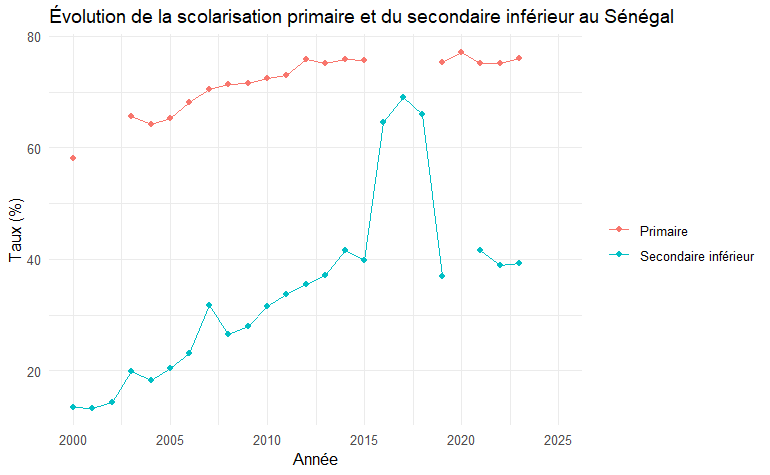
\includegraphics[width=0.8\textwidth]{Pictures/graphs/sdg4_primary_second.png}
	\caption{Taux de scolarisation primaire et achèvement du secondaire inférieur}
\end{figure}

\noindent
Les données disponibles indiquent une amélioration globale de l’accès à l’éducation de base au Sénégal. Le taux net de scolarisation primaire progresse d’environ 58 \% au début des années 2000 pour atteindre près de 76 \% sur les dernières années observées. De même, le taux d’achèvement du secondaire inférieur passe d’environ 13 \% à près de 39 \%, traduisant une amélioration de la rétention scolaire. Toutefois, la présence de valeurs manquantes sur certaines années invite à une lecture prudente des tendances de long terme.


\section*{Cible 4.2 : Éducation préscolaire}

La cible 4.2 de l’Objectif de Développement Durable 4 vise à garantir que toutes les filles et tous les garçons aient accès à des services de développement de la petite enfance et à une éducation préscolaire de qualité afin qu’ils soient prêts pour l’enseignement primaire. Dans ce cadre, l’indicateur retenu est le \textbf{taux de participation à l’enseignement préscolaire organisé}, correspondant au pourcentage d’enfants âgés de 4 à 6 ans inscrits dans un programme préscolaire formel.

L'indicateur \textbf{Participation à l'éducation préscolaire} mesure le pourcentage d'enfants âgés de 4 à 6 ans inscrits dans l'enseignement organisé avant l'école primaire. Il permet d'apprécier l'accès à l'éducation précoce, essentielle pour préparer les enfants à la scolarité obligatoire.

\begin{table}[H]
	\centering
	\caption{Taux de participation à l’enseignement préscolaire organisé au Sénégal}
	\begin{tabular}{cc}
		\hline
		\textbf{Année} & \textbf{Taux (\%)} \\
		\hline
		2000 & 13,8 \\
		2003 & 17,2 \\
		2005 & 7,3 \\
		2010 & 14,2 \\
		2015 & 18,5 \\
		2020 & 17,0 \\
		2023 & 22,7 \\
		\hline
	\end{tabular}
	\label{tab:preprimary}
\end{table}

\noindent
Les données disponibles indiquent une progression globale du taux de participation à l’enseignement préscolaire organisé au Sénégal, passant d’environ 14~\% au début des années 2000 à près de 23~\% sur les années les plus récentes observées. Cette évolution traduit les efforts consentis en matière de développement de la petite enfance. Toutefois, les niveaux demeurent relativement faibles au regard des ambitions de la cible 4.2, qui vise un accès universel à une éducation préscolaire de qualité.


\section*{Synthèse de la performance - ODD4}

\begin{figure}[H]
	\centering
	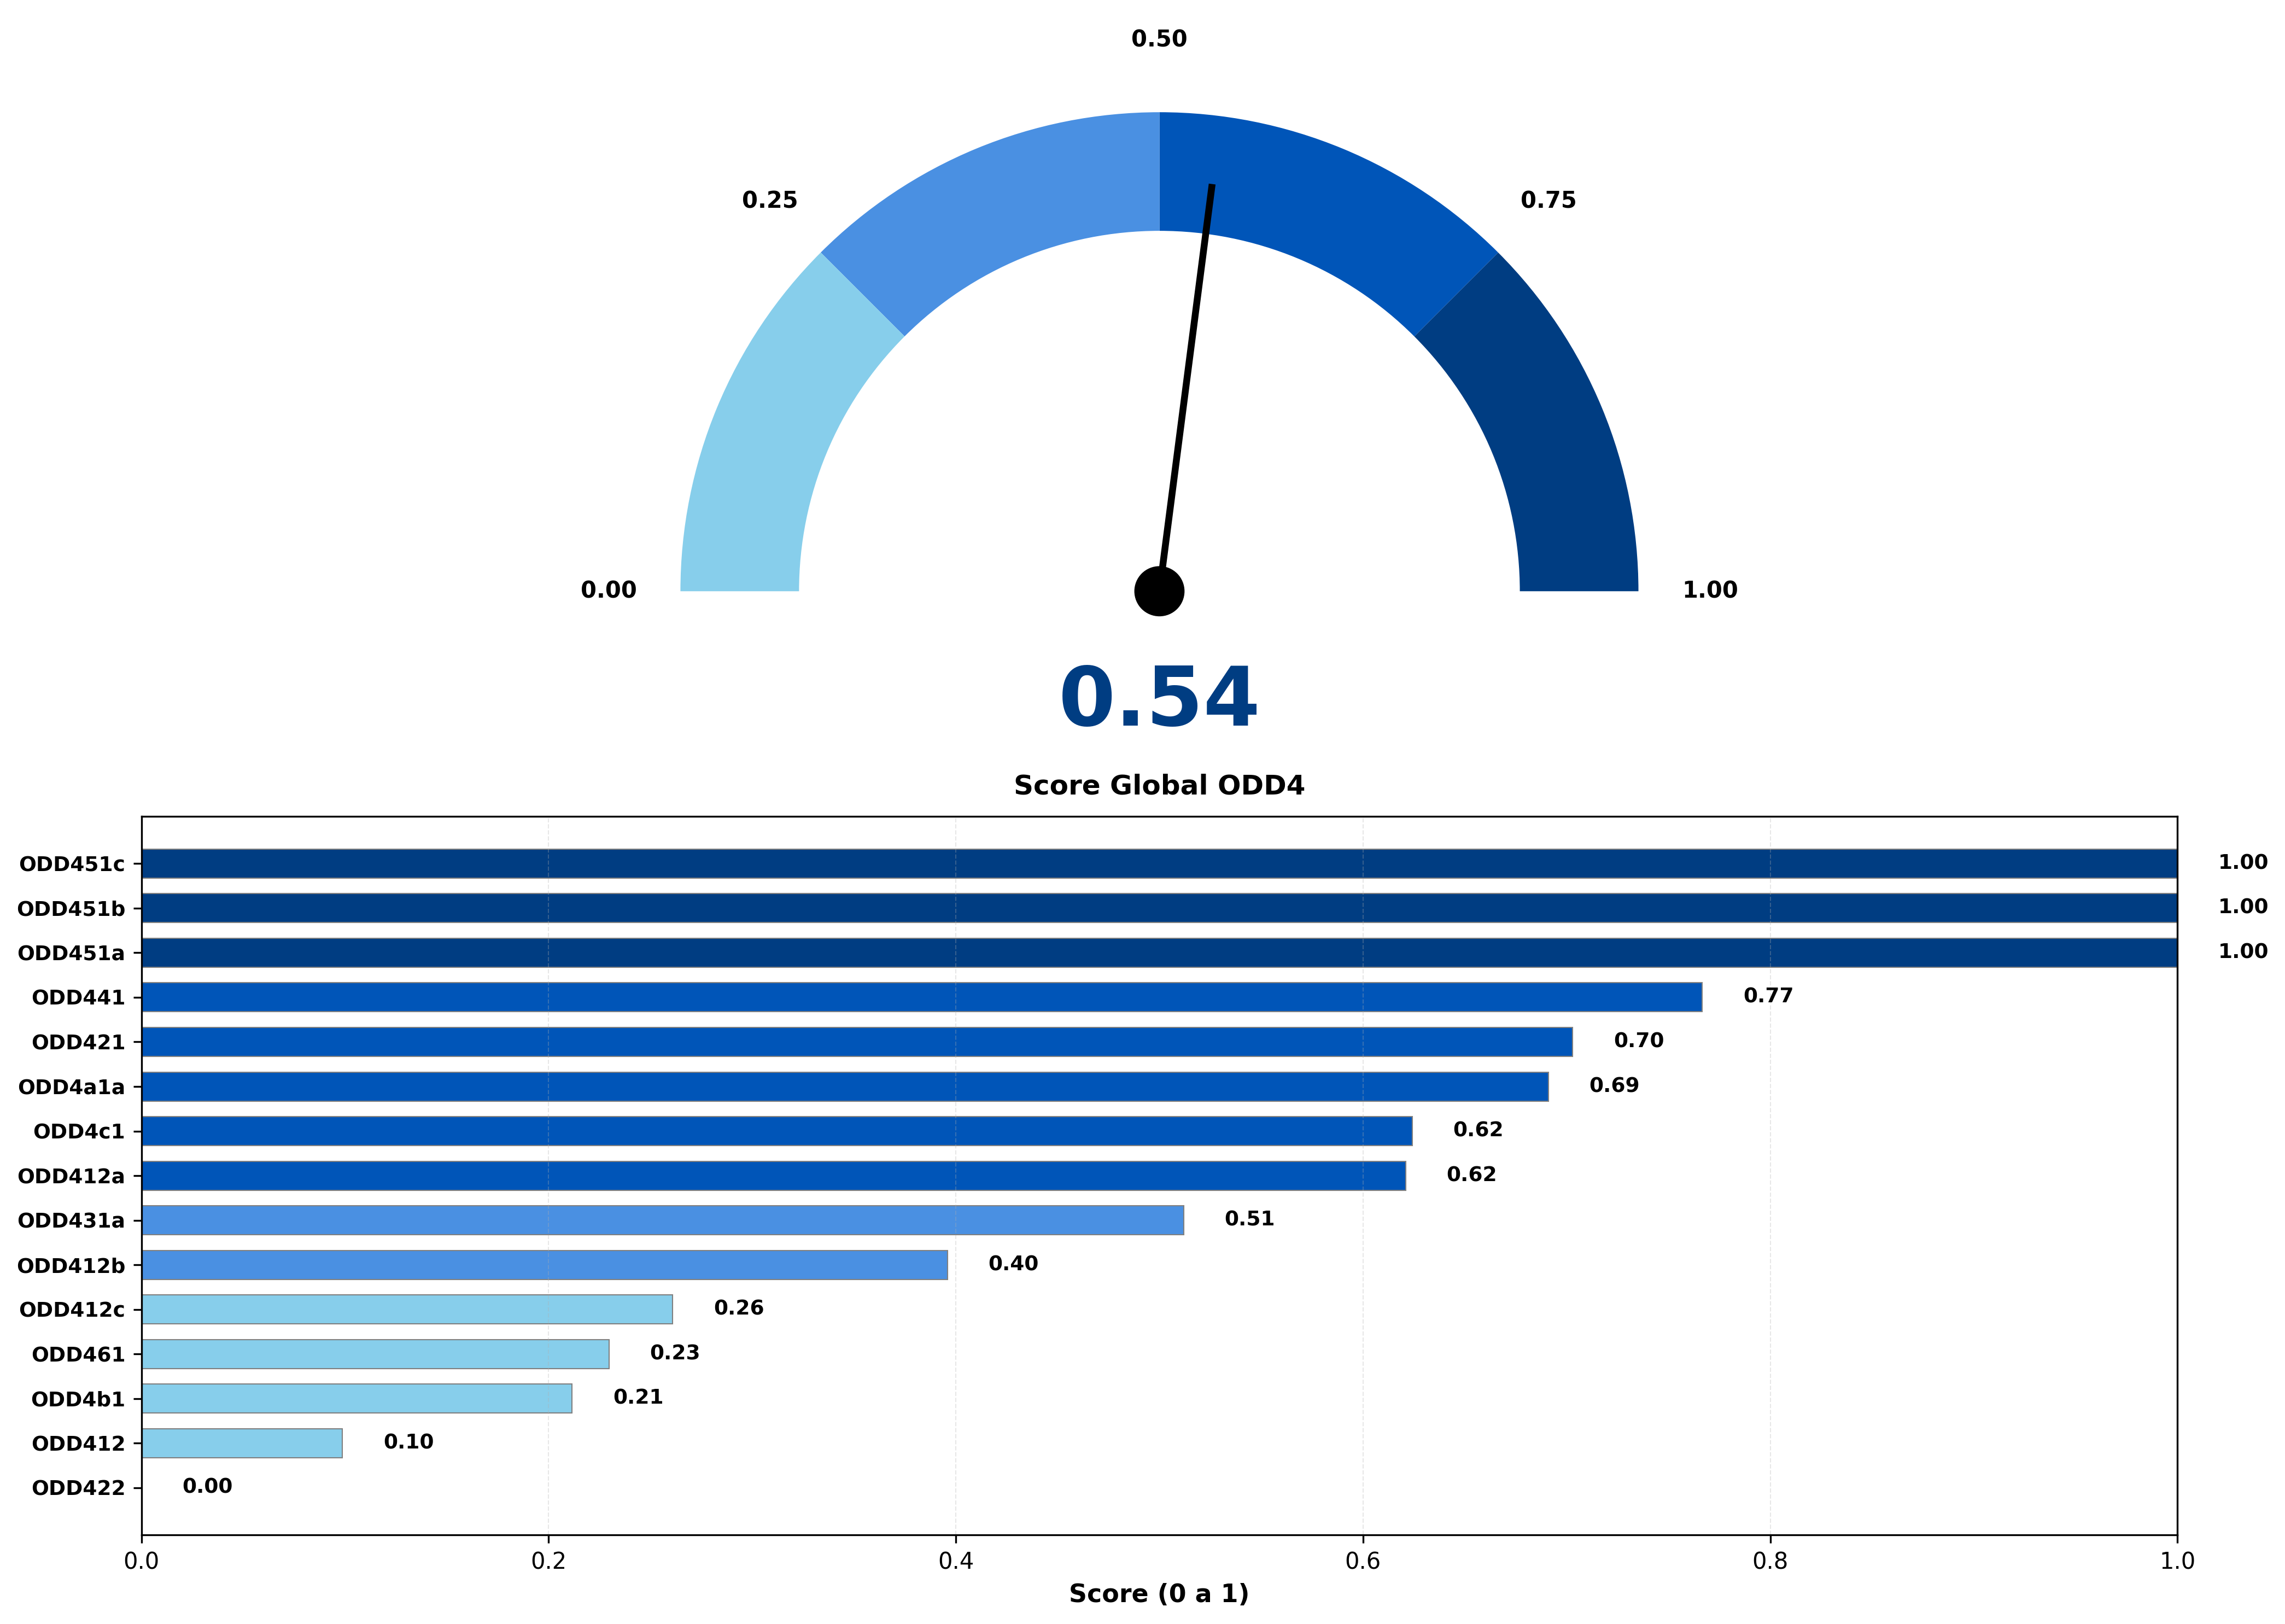
\includegraphics[width=0.95\textwidth]{Pictures/graphs/ODD4_scores.png}
	\caption{Performance par indicateur - ODD4}
\end{figure}

\begin{table}[H]
	\centering
	\begin{tabularx}{\textwidth}{l l c c c}s
		\rowcolor[HTML]{003D82}
		\color{white}\textbf{Code} & \color{white}\textbf{Indicateur} & \color{white}\textbf{Valeur} & \color{white}\textbf{Cible} & \color{white}\textbf{Score} \\
		\rowcolor[HTML]{F5F8FC}
		ODD422 & Participation à l'education prescolaire(4-6ans) & 0.23 & 1.00 & 0.00 \\
		\rowcolor[HTML]{E8F0FF}
		ODD412 & Taux d'achévement & 0.26 & 1.00 & 0.10 \\
		\rowcolor[HTML]{F5F8FC}
		ODD4b1 & Volume des dépenses en Education consacré aux bourse d'étude & 0.72 & 0.26 & 0.21 \\
		\rowcolor[HTML]{E8F0FF}
		ODD461 & Alphabétisation adulte & 0.55 & 0.90 & 0.23 \\
		\rowcolor[HTML]{F5F8FC}
		ODD412c & Taux d’achèvement en cycle secondaire & 0.26 & 1.00 & 0.26 \\
		\rowcolor[HTML]{E8F0FF}
		ODD412b & Taux d’achèvement au moyen & 0.40 & 1.00 & 0.40 \\
		\rowcolor[HTML]{F5F8FC}
		ODD431a & TBS à l'enseignement supérieur & 0.51 & 1.00 & 0.51 \\
		\rowcolor[HTML]{E8F0FF}
		ODD412a & Taux d’achèvement du cycle élèmentaire  & 0.62 & 1.00 & 0.62 \\
		\rowcolor[HTML]{F5F8FC}
		ODD4c1 & Proportion d'instituteurs formés & 0.15 & 0.24 & 0.62 \\
		\rowcolor[HTML]{E8F0FF}
		ODD4a1a & Etablissement scolaires et Electricité & 0.53 & 0.77 & 0.69 \\
		\rowcolor[HTML]{F5F8FC}
		ODD421 & Enfant de 5 ans en bonne voie & 0.70 & 1.00 & 0.70 \\
		\rowcolor[HTML]{E8F0FF}
		ODD441 & Compétences en informatique et en communication & 0.46 & 0.60 & 0.77 \\
		\rowcolor[HTML]{F5F8FC}
		ODD451a & Indice de parité du TBS à l’élémentaire & 1.20 & 1.00 & 1.00 \\
		\rowcolor[HTML]{E8F0FF}
		ODD451b & Indice de parité du TBS au moyen & 1.26 & 1.00 & 1.00 \\
		\rowcolor[HTML]{F5F8FC}
		ODD451c & Indice de parité du TBS au secondaire & 1.29 & 1.00 & 1.00 \\
	\end{tabularx}
\end{table}

L'analyse du ODD4 révèle un score global de 0.5410, basé sur 15 indicateur(s). Les performances varient de 0.00 à 1.00, montrant une certaine disparité dans la mise en oeuvre des cibles. Les indicateurs critiques (score < 0,30) nécessitent une attention particulière.


%%%%%%%%%%%%%%%%%%%%% ODD5 %%%%%%%%%%%%%%%%%%%%%%%%%%%

\newpages
\begin{simplebox2}
	
	\begin{minipage}{0.15\textwidth}
		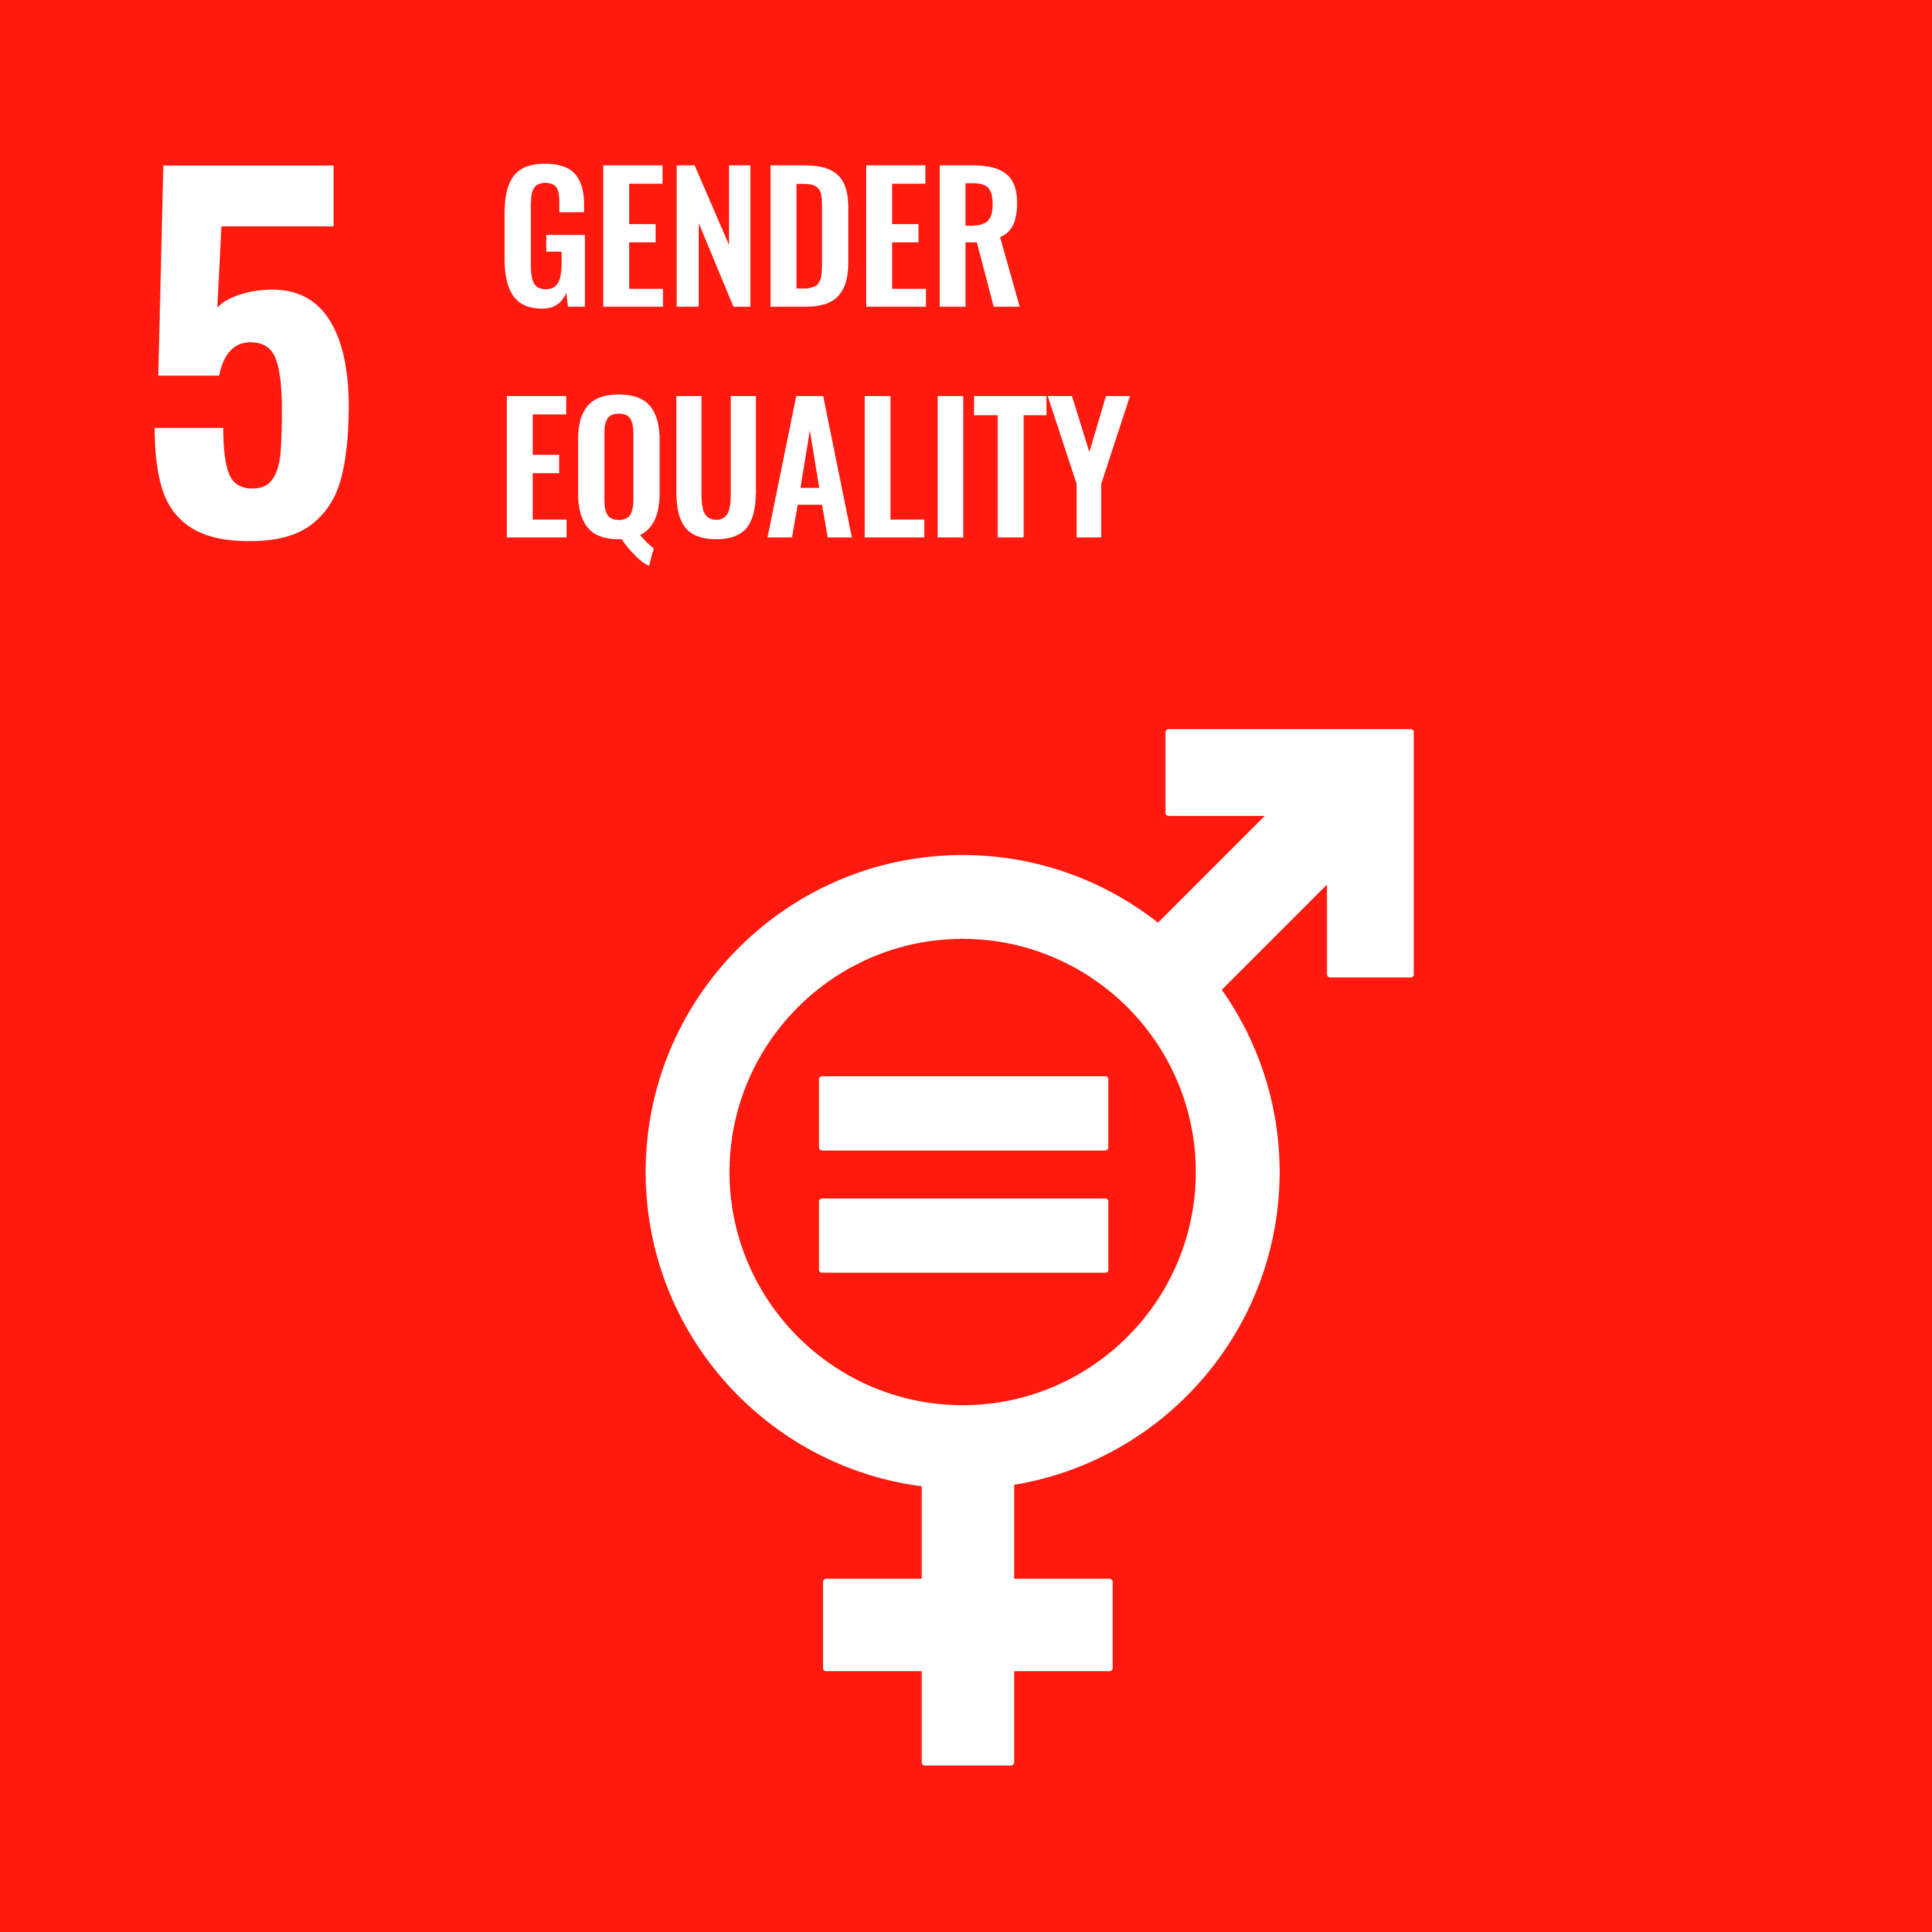
\includegraphics[width=\linewidth]{Pictures/ODD/ODD05.jpg}
	\end{minipage}
	\hfill
	\begin{minipage}{0.8\textwidth}
		{\bfseries\Large ODD 5 : }\\[2pt]
		\textit{ Parvenir à l’égalité des sexes et autonomiser toutes les femmes et les filles}
	\end{minipage}
\end{simplebox2}





\section*{Cible 5.5 : Participation politique et économique des femmes}

La cible 5.5 vise à assurer la participation pleine et effective des femmes à la vie politique et publique, ainsi que l’égalité des chances dans la prise de décision et l’accès aux postes de responsabilité.  
Un indicateur clé pour suivre cette cible est le \textbf{pourcentage de sièges occupés par des femmes au parlement national}, qui refslète la représentation politique et l’influence des femmes dans les instances décisionnelles.

\begin{figure}[H]
	\centering
	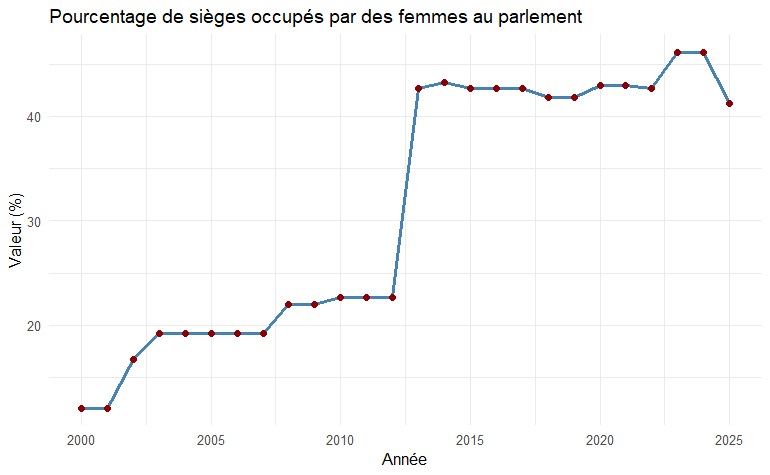
\includegraphics[width=0.8\textwidth]{Pictures/graphs/sdg5_parl.png}
	\caption{Pourcentage de sièges occupés par des femmes au parlement national au Sénégal (2000-2025)}
\end{figure}

\noindent
Les données montrent une évolution positive de la représentation des femmes au parlement au Sénégal. En 2000, seulement 12~\% des sièges étaient occupés par des femmes. Cette proportion a augmenté progressivement pour atteindre 22~\% au début des années 2010, puis un pic de 43~\% pour certaines années récentes.  

Cette progression traduit les efforts déployés pour promouvoir l’égalité des sexes dans la sphère politique, notamment grâce à des politiques et mesures incitatives visant à renforcer la présence des femmes. Toutefois, les fluctuations observées sur les dernières années indiquent que des efforts soutenus restent nécessaires pour atteindre une représentation stable et équilibrée.


\section*{Cible 5.6 : Accès à la santé sexuelle et reproductive}

La cible 5.6 vise à assurer l’accès universel à la santé sexuelle et reproductive et aux droits reproductifs. L’indicateur disponible est :  

\begin{itemize}
	\item \textbf{Demande de planification familiale satisfaite par des méthodes modernes (\% de femmes âgées de 15 à 49 ans)}
\end{itemize}

\begin{figure}[H]
	\centering
	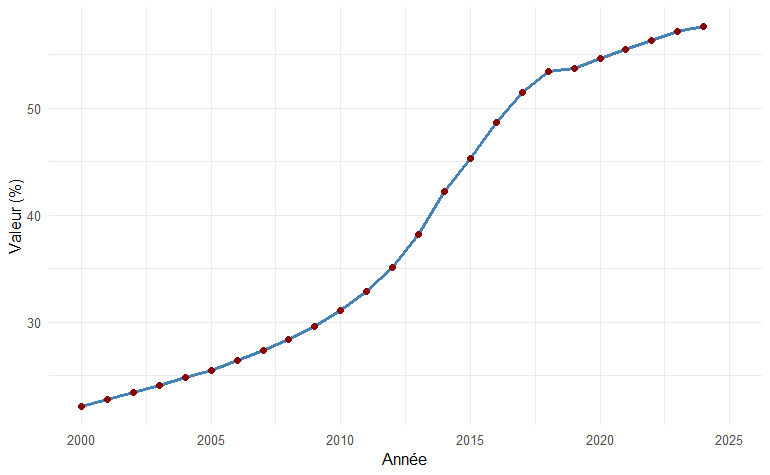
\includegraphics[width=0.8\textwidth]{Pictures/graphs/sdg5_familyplanning.png}
	\caption{Demande de planification familiale satisfaite par des méthodes modernes (2000-2025)}
\end{figure}

\noindent
Le taux de satisfaction de la demande de planification familiale a progressé régulièrement, passant de 22~\% au début des années 2000 à près de 58~\% sur les dernières années observées, traduisant une amélioration significative de l’accès aux services de santé reproductive.


\section*{Synthèse de la performance - ODD5}

\begin{figure}[H]
	\centering
	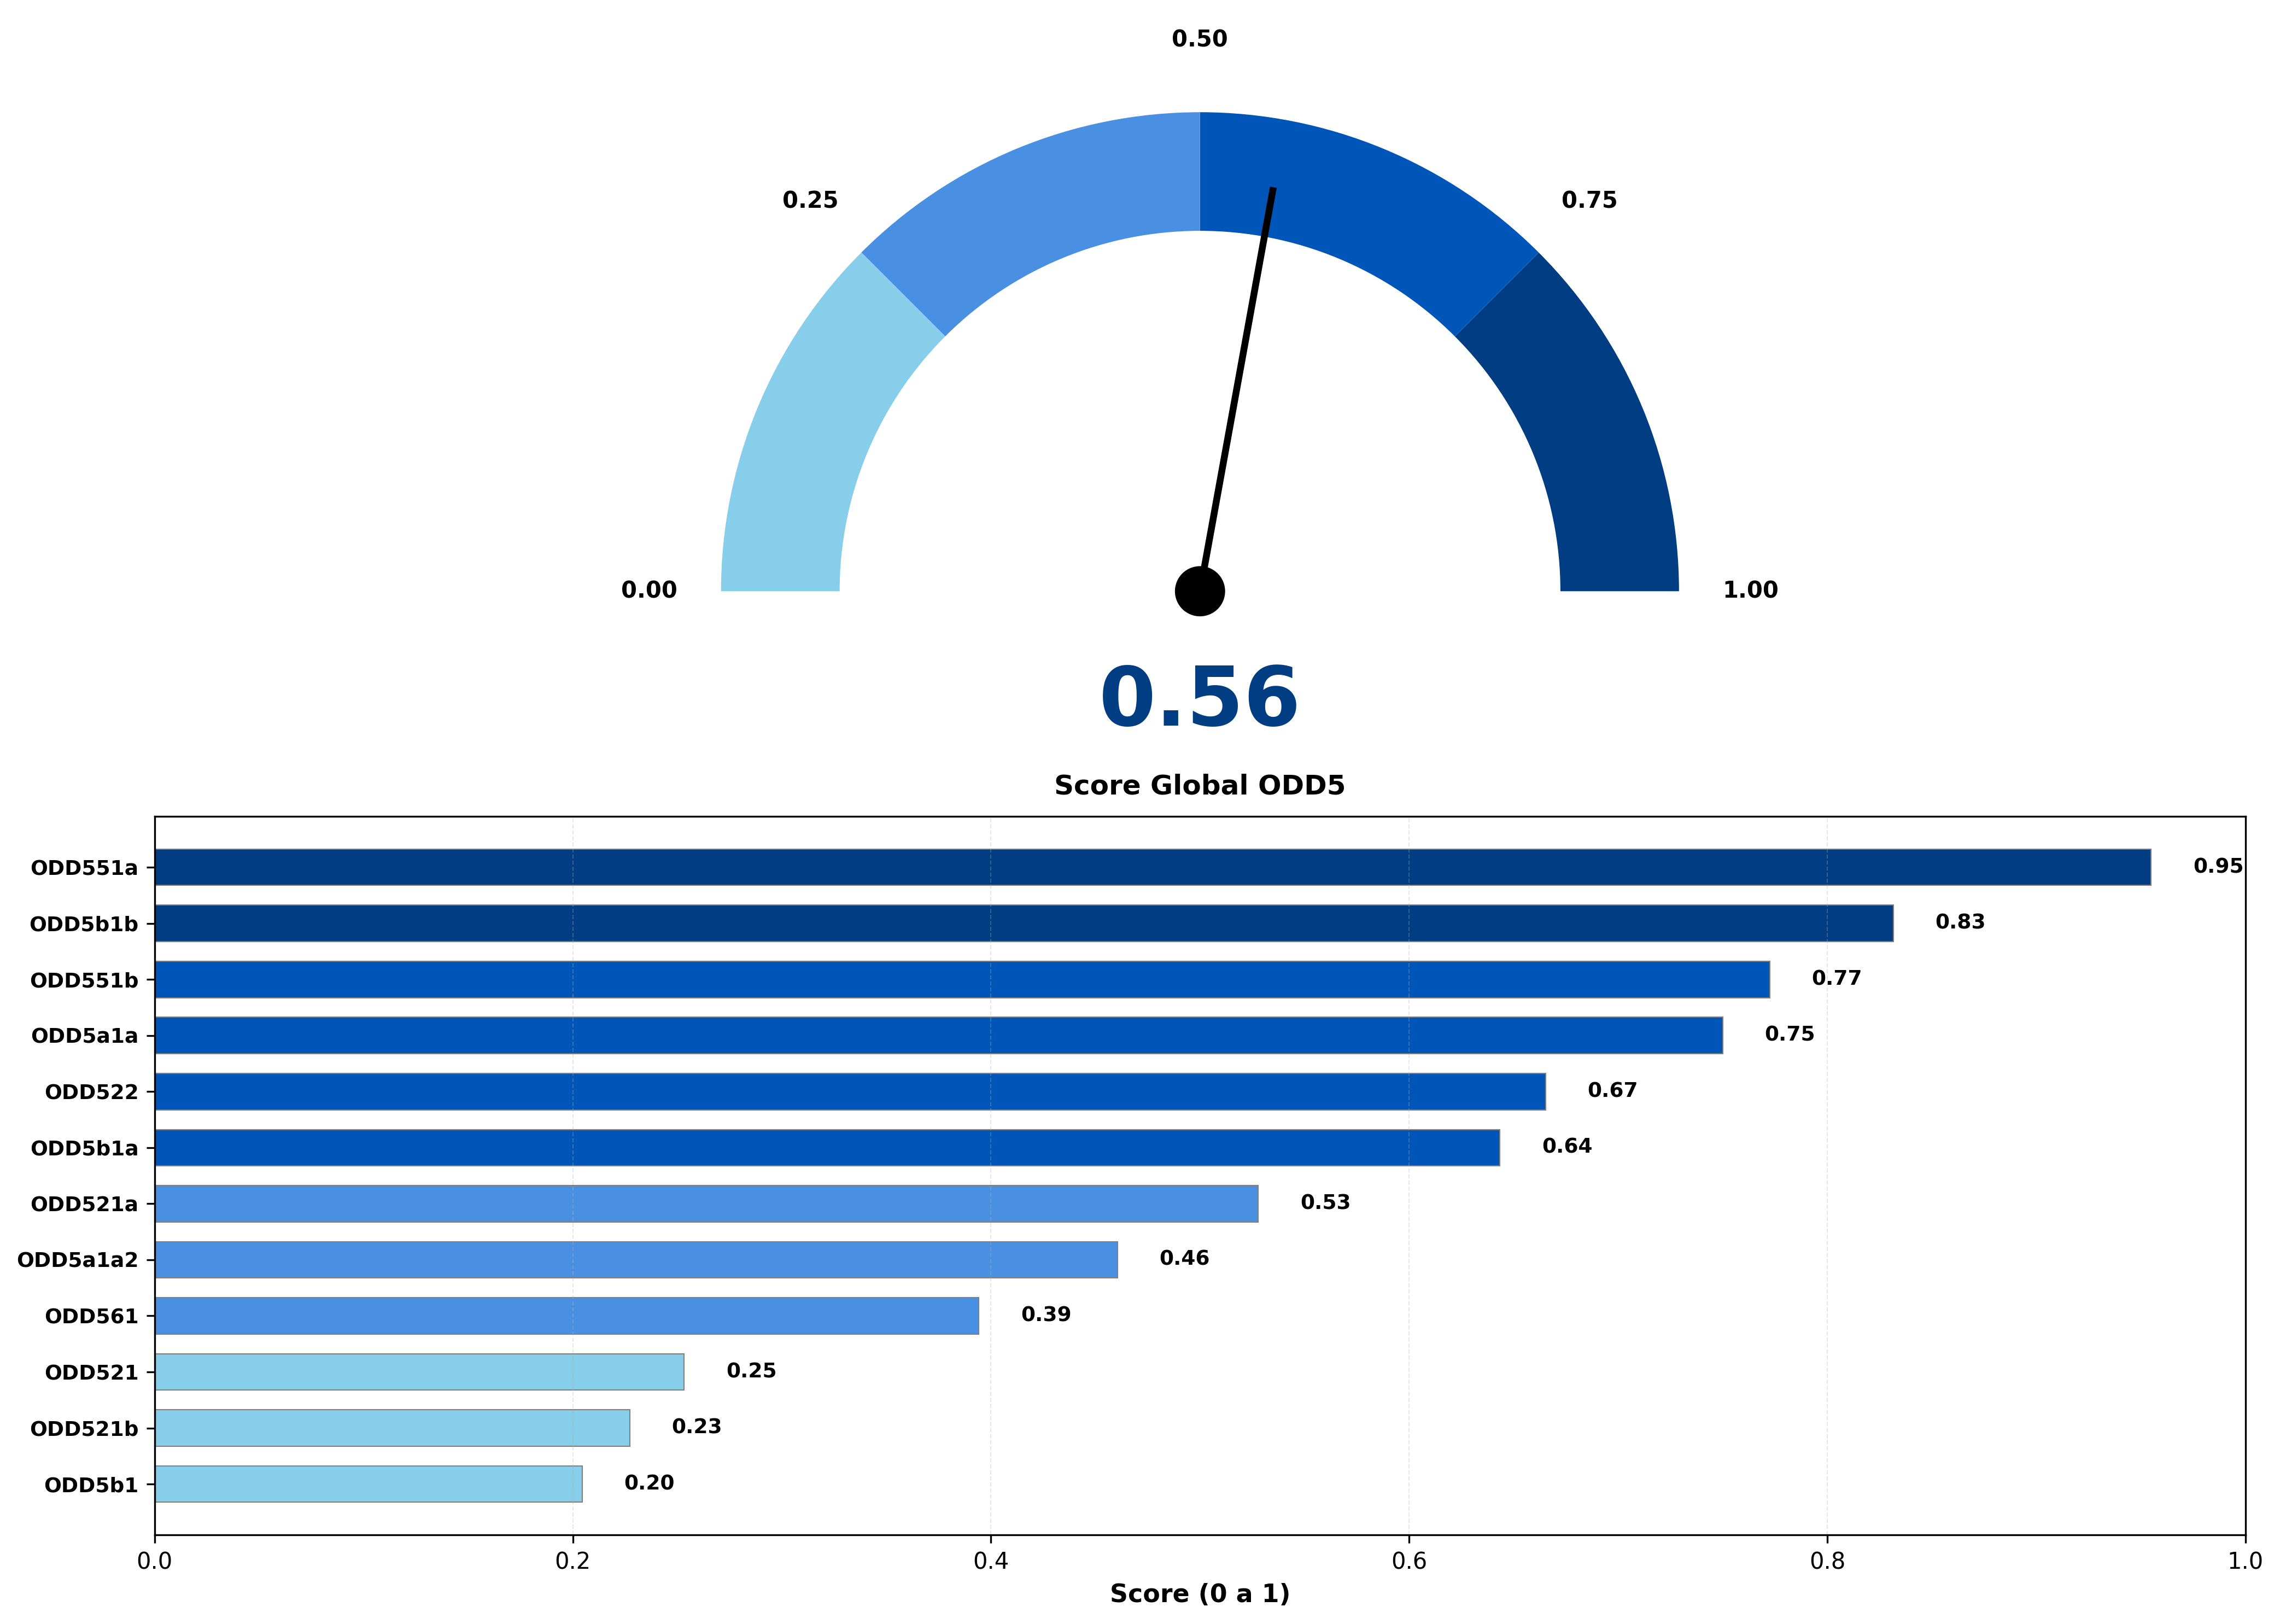
\includegraphics[width=0.95\textwidth]{Pictures/graphs/ODD5_scores.png}
	\caption{Performance par indicateur - ODD5}
\end{figure}

\begin{table}[H]
	\centering
	\begin{tabularx}{\textwidth}{l l c c c}
		\rowcolor[HTML]{003D82}
		\color{white}\textbf{Code} & \color{white}\textbf{Indicateur} & \color{white}\textbf{Valeur} & \color{white}\textbf{Cible} & \color{white}\textbf{Score} \\
		\rowcolor[HTML]{F5F8FC}
		ODD5b1 & Taux de pénétration de la téléphonie mobile & 0.44 & 1.00 & 0.20 \\
		\rowcolor[HTML]{E8F0FF}
		ODD521b & Femmes de 20–24 ans ayant été mariées ou en u & 0.31 & 0.00 & 0.23 \\
		\rowcolor[HTML]{F5F8FC}
		ODD521 & Violence des filles et des femmes & 0.22 & 0.00 & 0.25 \\
		\rowcolor[HTML]{E8F0FF}
		ODD561 & Décisions informées concernant les relations sex & 0.58 & 1.00 & 0.39 \\
		\rowcolor[HTML]{F5F8FC}
		ODD5a1a2 & Femmes titulaires de droits de propriétés & 0.08 & 0.17 & 0.46 \\
		\rowcolor[HTML]{E8F0FF}
		ODD521a & Femmes de 20–24 ans ayant été mariées ou en u & 0.09 & 0.00 & 0.53 \\
		\rowcolor[HTML]{F5F8FC}
		ODD5b1a & Possession de téléphone portable & 0.75 & 1.00 & 0.64 \\
		\rowcolor[HTML]{E8F0FF}
		ODD522 & Mutilation génitale féminine & 0.20 & 0.00 & 0.67 \\
		\rowcolor[HTML]{F5F8FC}
		ODD5a1a & Population Agricole titulaires des droits de propriété & 0.75 & 1.00 & 0.75 \\
		\rowcolor[HTML]{E8F0FF}
		ODD551b & Femmes dans les Bureaux des conseils territoriaux & 0.39 & 0.50 & 0.77 \\
		\rowcolor[HTML]{F5F8FC}
		ODD5b1b & Possession de téléphone portable par les hommes & 0.88 & 1.00 & 0.83 \\
		\rowcolor[HTML]{E8F0FF}
		ODD551a & Femmes dans les effectifs des conseils territoriaux & 0.48 & 0.50 & 0.95 \\
	\end{tabularx}
\end{table}

L'analyse du ODD5 révèle un score global de 0.5572, basé sur 12 indicateur(s). Les performances varient de 0.20 à 0.95, montrant une certaine disparité dans la mise en oeuvre des cibles. Les indicateurs critiques (score < 0,30) nécessitent une attention particulière.

%%%%%%%%%%%%%%%%%%%%% ODD6 %%%%%%%%%%%%%%%%%%%%%%%%%%%

\newpage
\begin{simplebox2}
	
	\begin{minipage}{0.15\textwidth}
		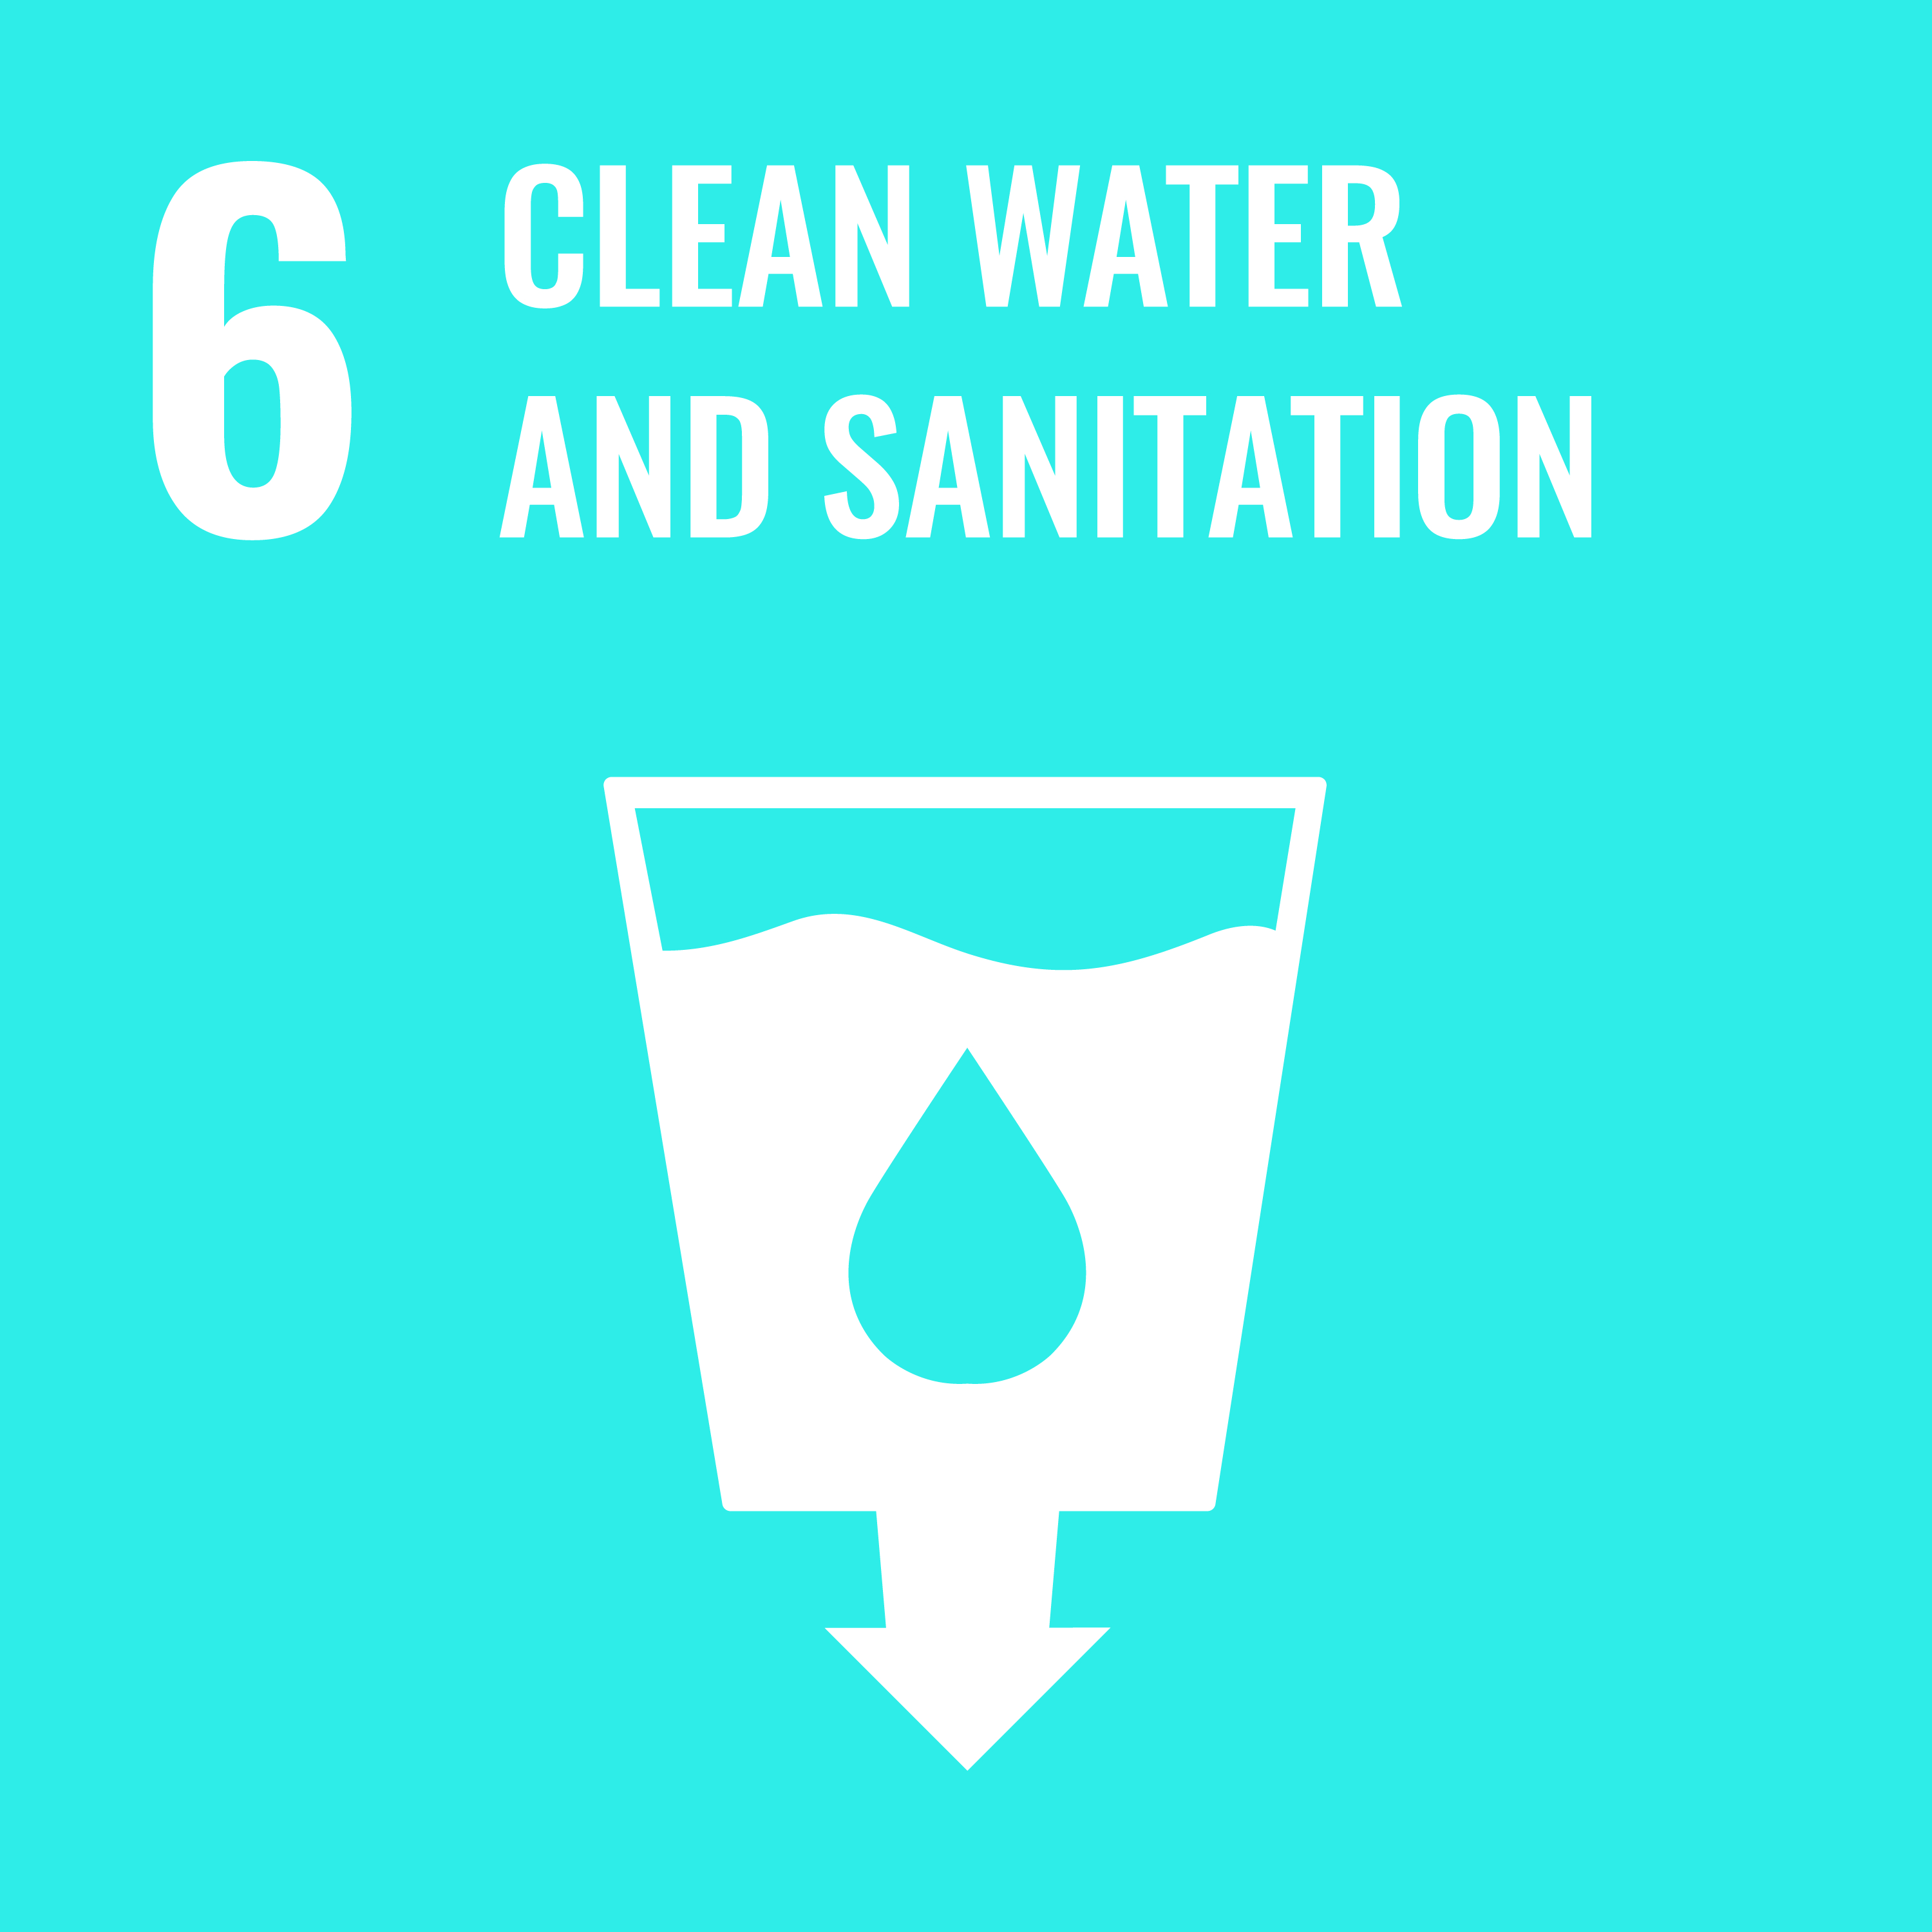
\includegraphics[width=\linewidth]{Pictures/ODD/ODD06.jpg}
	\end{minipage}
	\hfill
	\begin{minipage}{0.8\textwidth}
		{\bfseries\Large ODD 6 : }\\[2pt]
		\textit{Garantir l’accès de tous à l’eau et à l’assainissement et assurer une gestion durable des ressources en eau}
	\end{minipage}
\end{simplebox2}




L’Objectif de Développement Durable 6 (ODD 6) vise à garantir l’accès universel à l’eau potable et à l’assainissement, ainsi qu’à assurer une gestion durable des ressources en eau. Cet objectif constitue un pilier fondamental du développement humain, de la santé publique et de la durabilité environnementale.

\section{Cible 6.1 : Accès universel à l’eau potable}

La cible 6.1 vise à garantir, d’ici 2030, l’accès universel et équitable à une eau potable salubre et abordable pour tous.

L’indicateur mobilisé est la proportion de la population utilisant au moins des services élémentaires d’eau potable. Les données montrent une amélioration continue de l’accès à l’eau potable au fil du temps. Toutefois, malgré cette progression, des écarts persistent, traduisant des inégalités structurelles dans l’accès aux infrastructures hydrauliques.

\begin{figure}[H]
	\centering
	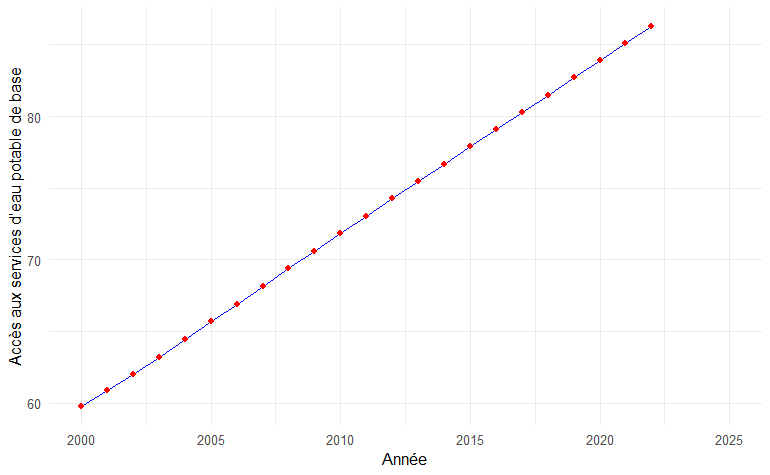
\includegraphics[width=0.8\textwidth]{Pictures/graphs/sdg6_water.png}
	\caption{Évolution de l’accès aux services d’eau potable de base}
	\label{fig:sdg6_1}
\end{figure}

La proportion de la population utilisant au moins des services élémentaires d’eau potable connaît une progression continue entre 2000 et 2025. Elle passe d’environ 60~\% au début de la période à plus de 86~\% sur les dernières années observées. Cette évolution traduit des avancées significatives dans le déploiement des infrastructures hydrauliques. Toutefois, l’écart entre l’accès de base et l’accès à des services d’eau gérés en toute sécurité demeure important.

\section{Cible 6.2 : Accès à l’assainissement et à l’hygiène}

La cible 6.2 vise à assurer l’accès de tous à des services d’assainissement et d’hygiène adéquats et équitables.

L’indicateur retenu est la proportion de la population utilisant au moins des services d’assainissement de base. Les résultats indiquent une progression régulière de l’accès à l’assainissement, bien que cette évolution demeure plus lente que celle observée pour l’eau potable, reflétant un retard structurel dans les investissements en assainissement.



L’accès aux services d’assainissement de base s’améliore également de manière régulière, passant d’environ 37~\% en 2000 à près de 60~\% en 2025. Malgré cette progression, le niveau reste relativement faible comparativement à l’accès à l’eau potable, soulignant un retard structurel dans les investissements en assainissement.
	
\section{Cible 6.4 : Gestion durable des ressources en eau}

La cible 6.4 vise à accroître l’efficacité de l’utilisation de l’eau et à garantir des prélèvements durables afin de réduire le stress hydrique.

L’indicateur utilisé est le prélèvement d’eau douce exprimé en pourcentage des ressources renouvelables disponibles. Les données révèlent une pression croissante sur les ressources en eau, ce qui soulève des enjeux importants de durabilité, notamment dans les contextes de forte demande agricole et industrielle.

\begin{figure}[H]
	\centering
	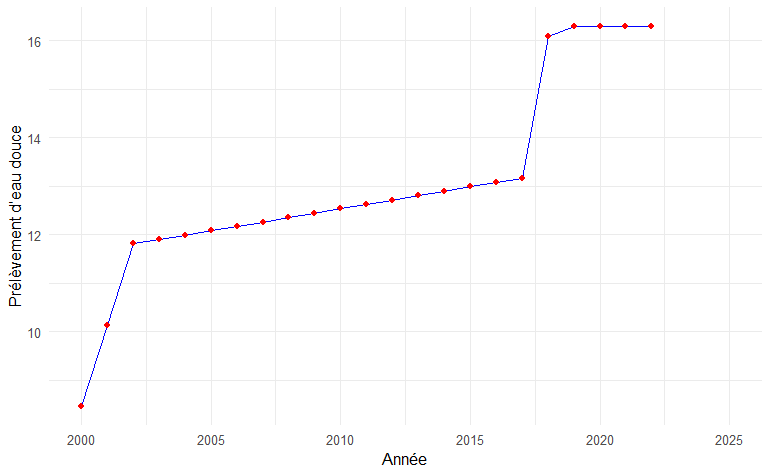
\includegraphics[width=0.8\textwidth]{Pictures/graphs/sdg6_freshwat.png}
	\caption{Évolution du prélèvement d’eau douce (\% des ressources disponibles)}
		\label{fig:sdg6_4}
\end{figure}

Le prélèvement d’eau douce, exprimé en pourcentage des ressources renouvelables disponibles, augmente sur la période étudiée. Cette tendance indique une pression croissante sur les ressources en eau, susceptible d’accroître les risques de stress hydrique à moyen et long terme si des mesures de gestion durable ne sont pas renforcées.


\section*{Synthèse de la performance - ODD6}

\begin{figure}[H]
	\centering
	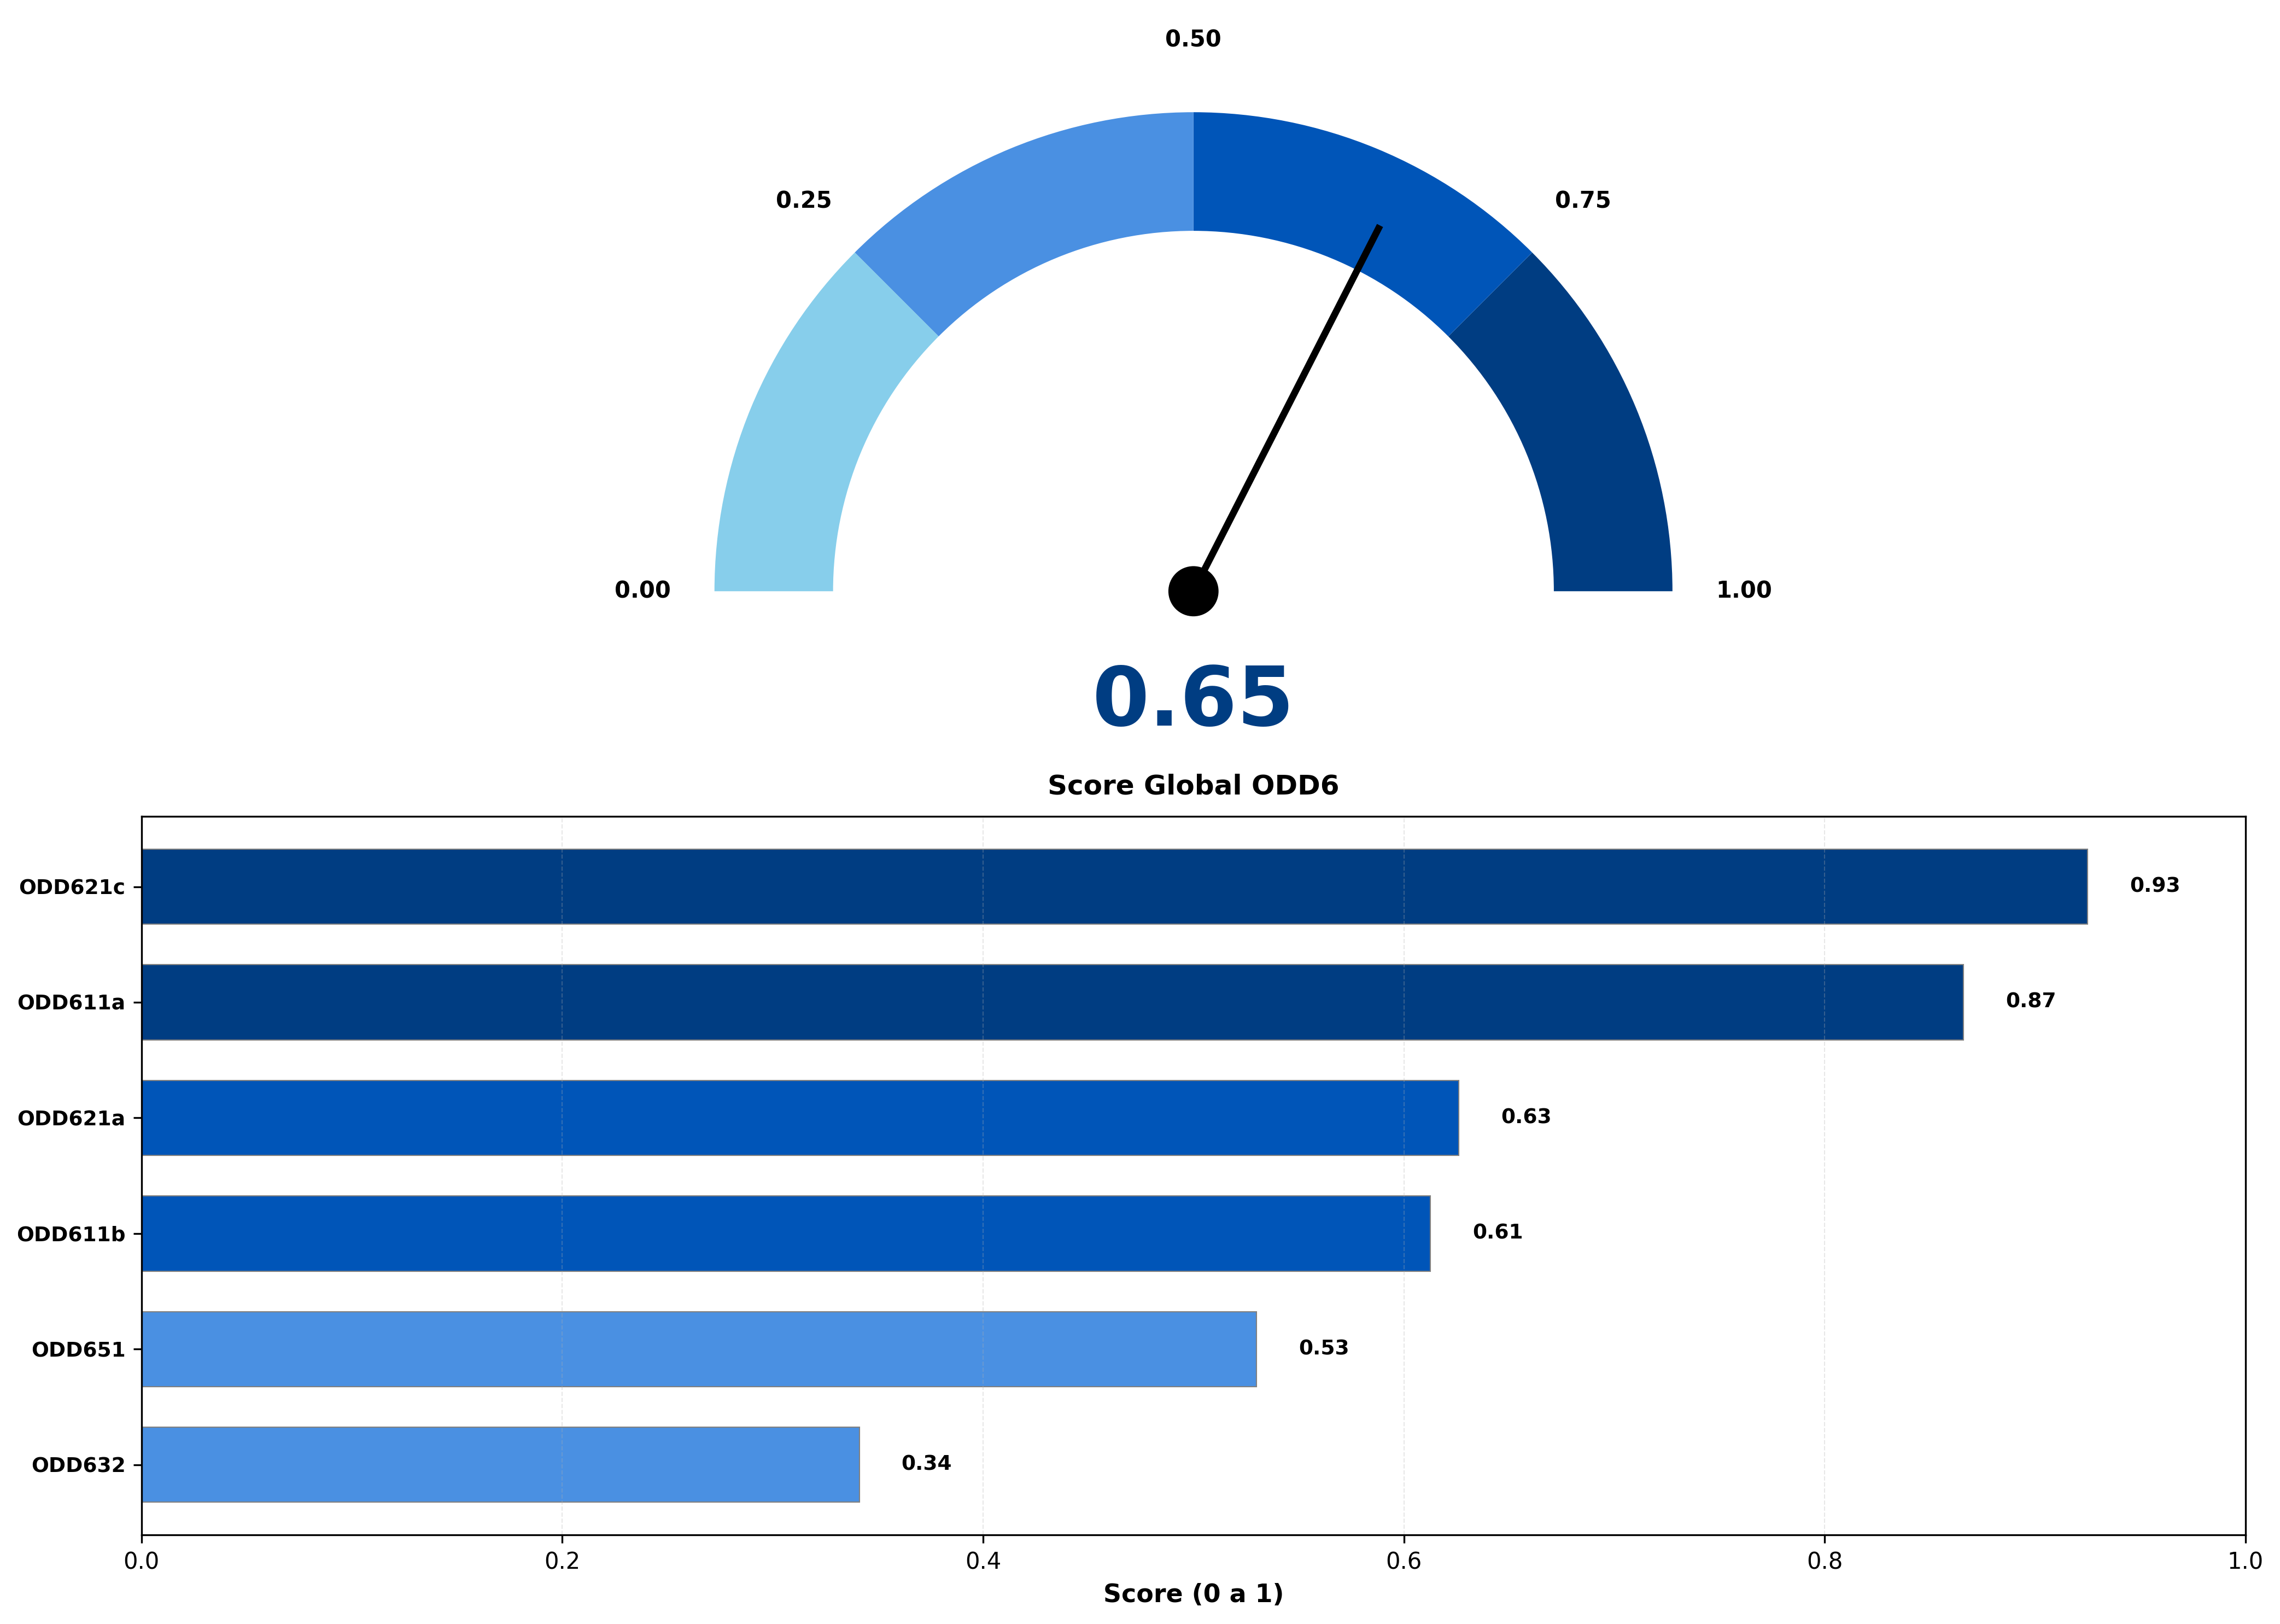
\includegraphics[width=0.95\textwidth]{Pictures/graphs/ODD6_scores.png}
	\caption{Performance par indicateur - ODD6}
\end{figure}

\begin{table}[H]
	\centering
	\begin{tabularx}{\textwidth}{l l c c c}
		\rowcolor[HTML]{003D82}
		\color{white}\textbf{Code} & \color{white}\textbf{Indicateur} & \color{white}\textbf{Valeur} & \color{white}\textbf{Cible} & \color{white}\textbf{Score} \\
		\rowcolor[HTML]{F5F8FC}
		ODD632 & Plans d'eau dont la qualité de l'eau est ambiante & 0.44 & 1.00 & 0.34 \\
		\rowcolor[HTML]{E8F0FF}
		ODD651 & Degré de mise en œuvre de la gestion intégrée des ressources en eau  & 0.53 & 1.00 & 0.53 \\
		\rowcolor[HTML]{F5F8FC}
		ODD611b & Accès aux services de base pour l'eau de boisson  & 0.61 & 1.00 & 0.61 \\
		\rowcolor[HTML]{E8F0FF}
		ODD621a & Accès aux services de base d'assainissement & 0.63 & 1.00 & 0.63 \\
		\rowcolor[HTML]{F5F8FC}
		ODD611a & Accès aux services de base pour l'eau de boisson & 0.87 & 1.00 & 0.87 \\
		\rowcolor[HTML]{E8F0FF}
		ODD621c & Défécation à l'air libre & 0.07 & 0.00 & 0.93 \\
	\end{tabularx}
\end{table}

L'analyse du ODD6 révèle un score global de 0.6501, basé sur 6 indicateur(s). Les performances varient de 0.34 à 0.93, montrant une certaine disparité dans la mise en oeuvre des cibles. Les indicateurs critiques (score < 0,30) nécessitent une attention particulière.


%%%%%%%%%%%%%%%%%%%%% ODD7 %%%%%%%%%%%%%%%%%%%%%%%%%%%

\newpage
\begin{simplebox2}
	
	\begin{minipage}{0.15\textwidth}
		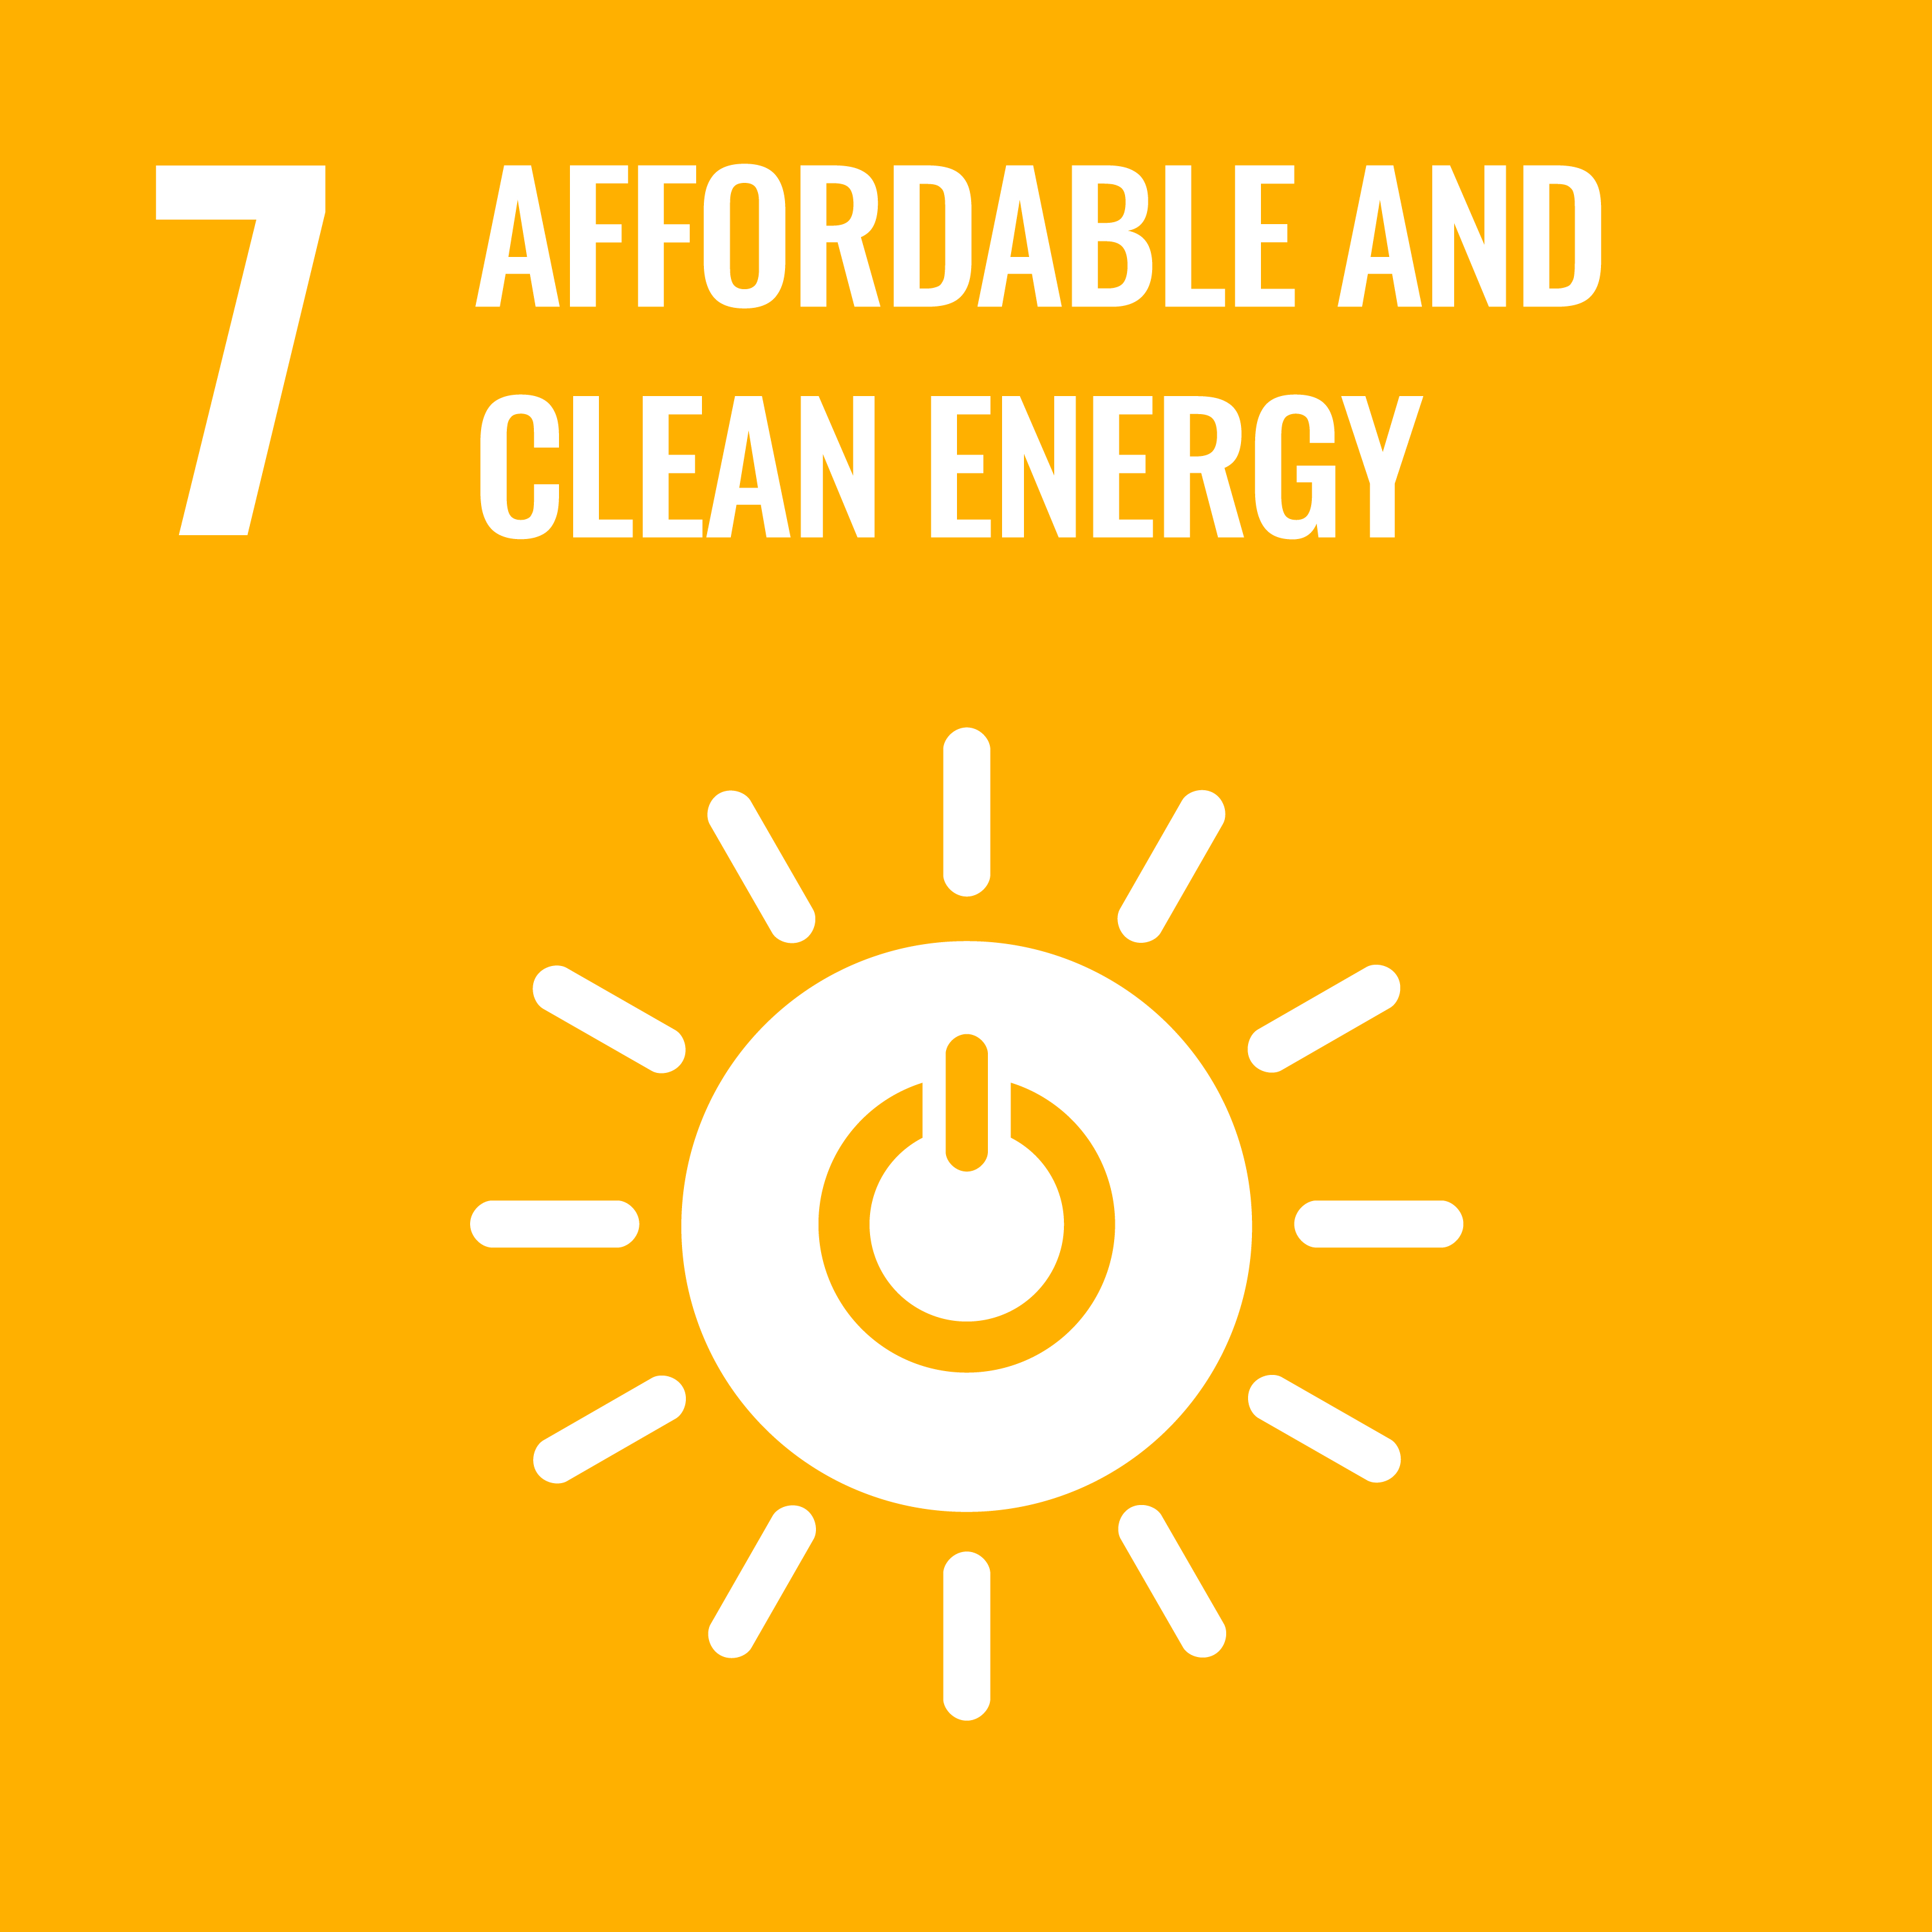
\includegraphics[width=\linewidth]{Pictures/ODD/ODD07.jpg}
	\end{minipage}
	\hfill
	\begin{minipage}{0.8\textwidth}
		{\bfseries\Large ODD 7 : }\\[2pt]
		\textit{Garantir l’accès de tous à des services énergétiques fiables, durables et modernes, à un coût abordable.}
	\end{minipage}
\end{simplebox2}



L’Objectif de Développement Durable 7 vise à garantir l’accès de tous à des services énergétiques fiables, durables et modernes, à un coût abordable. Dans cette analyse, l’attention est portée sur les cibles \textbf{7.1} et \textbf{7.2}, pour lesquelles des indicateurs quantitatifs sont disponibles.

\section*{Cible 7.1 : Accès universel à des services énergétiques modernes}

La cible 7.1 a pour objectif de garantir, d’ici à 2030, l’accès universel à des services énergétiques fiables, durables et modernes. Cette dimension est appréhendée ici par la proportion de la population ayant accès à l’électricité.

\begin{figure}[H]
	\centering
	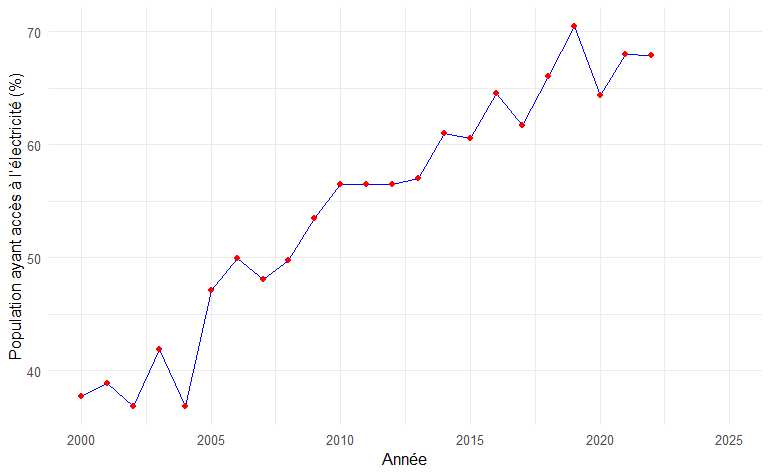
\includegraphics[width=0.8\textwidth]{Pictures/graphs/sdg7__elecac.png}
	\caption{Évolution de la population ayant accès à l'électricité}
	\label{fig:sdg7_1}
\end{figure}

Les résultats montrent une amélioration progressive de l’accès à l’électricité au fil du temps, passant de 36,8\% à 70,4\% entre 2000 et 2022, traduisant les efforts consentis en matière d’électrification. 
Cependant, malgré ces progrès significatifs, une proportion non négligeable de la population demeure privée d’accès à l’électricité.
Cela souligne que des efforts supplémentaires sont nécessaires pour atteindre l’objectif de couverture universelle fixé par la cible 7.1, afin que l’ensemble de la population bénéficie d’un accès fiable et durable aux services énergétiques.



\section*{Synthèse de la performance - ODD7}

\begin{figure}[H]
	\centering
	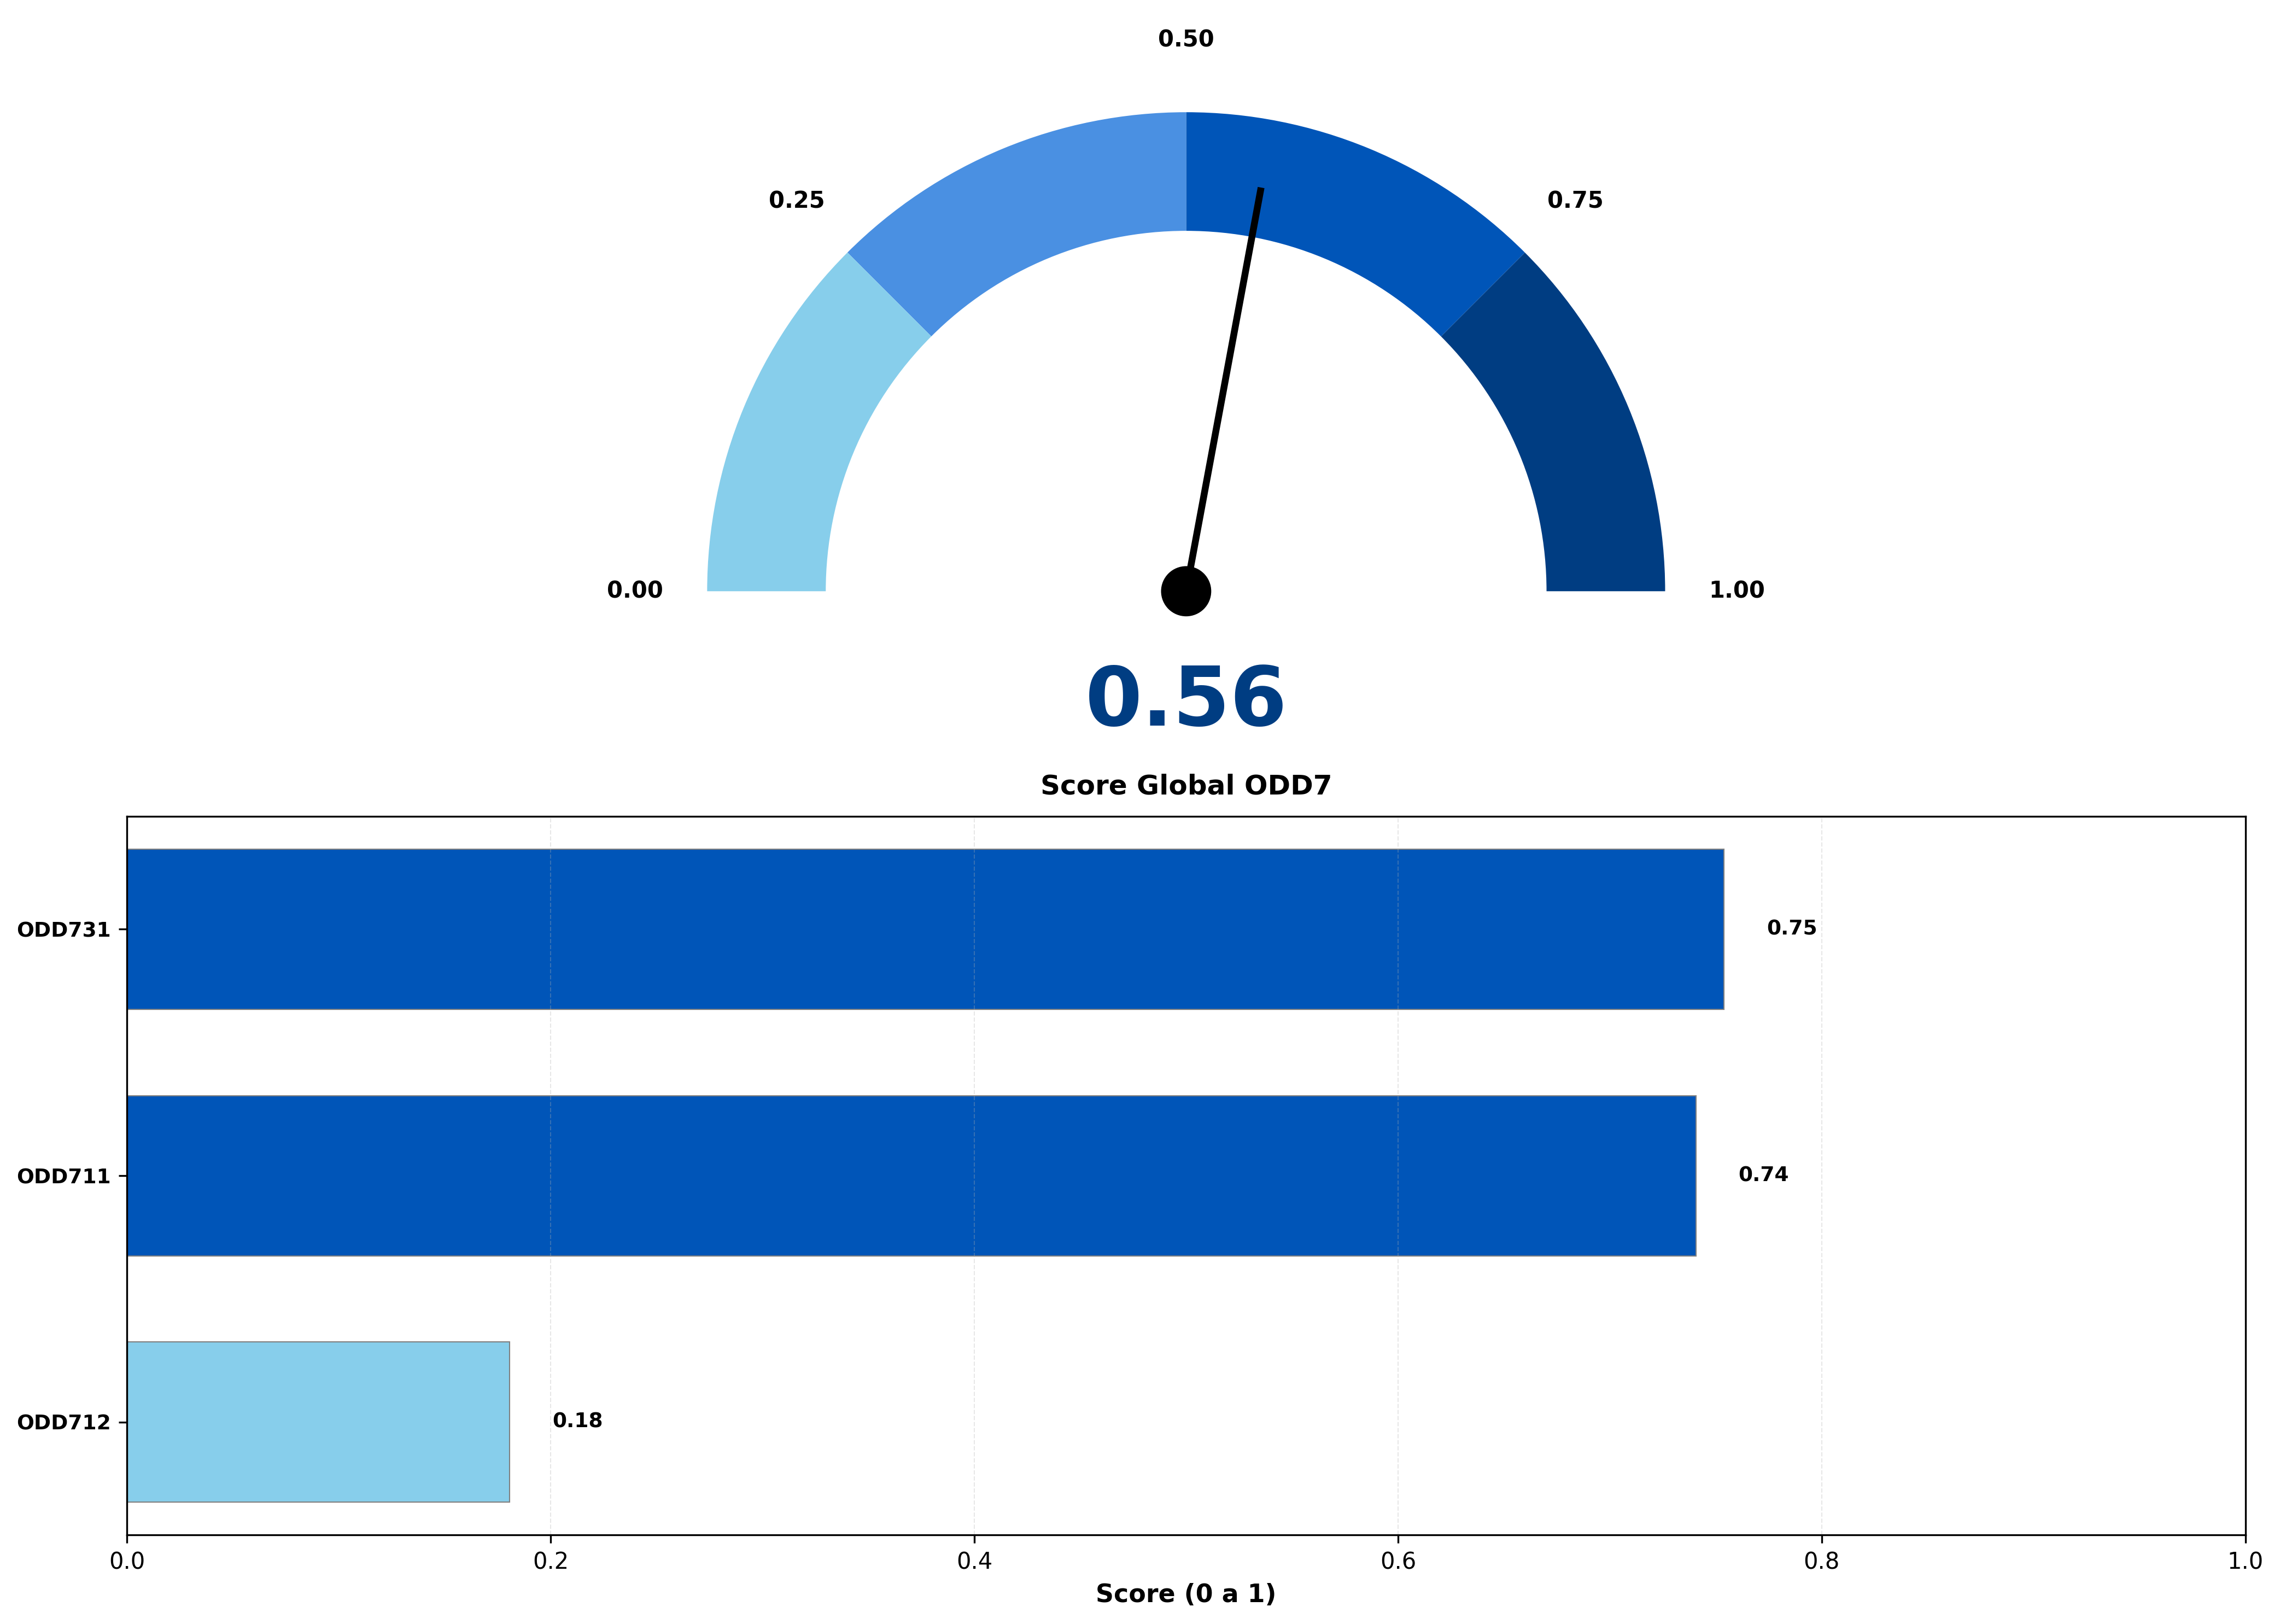
\includegraphics[width=0.95\textwidth]{Pictures/graphs/ODD7_scores.png}
	\caption{Performance par indicateur - ODD7}
\end{figure}

\begin{table}[H]
	\centering
	\begin{tabularx}{\textwidth}{l l c c c}
		\rowcolor[HTML]{003D82}
		\color{white}\textbf{Code} & \color{white}\textbf{Indicateur} & \color{white}\textbf{Valeur} & \color{white}\textbf{Cible} & \color{white}\textbf{Score} \\
		\rowcolor[HTML]{F5F8FC}
		ODD712 & Accès aux énergies et technologies propres & 0.20 & 1.00 & 0.18 \\
		\rowcolor[HTML]{E8F0FF}
		ODD711 & Accès à l'électricité & 0.76 & 1.00 & 0.74 \\
		\rowcolor[HTML]{F5F8FC}
		ODD731 & Intensité énergétique (rapport entre énergie primaire et PIB) & 0.01 & 0.00 & 0.75 \\
	\end{tabularx}
\end{table}

L'analyse du ODD7 révèle un score global de 0.5584, basé sur 3 indicateur(s). Les performances varient de 0.18 à 0.75, montrant une certaine disparité dans la mise en oeuvre des cibles. Les indicateurs critiques (score < 0,30) nécessitent une attention particulière.


%%%%%%%%%%%%%%%%%%%%% ODD8 %%%%%%%%%%%%%%%%%%%%%%%%%%%

\newpage
\begin{simplebox2}
	
	\begin{minipage}{0.15\textwidth}
		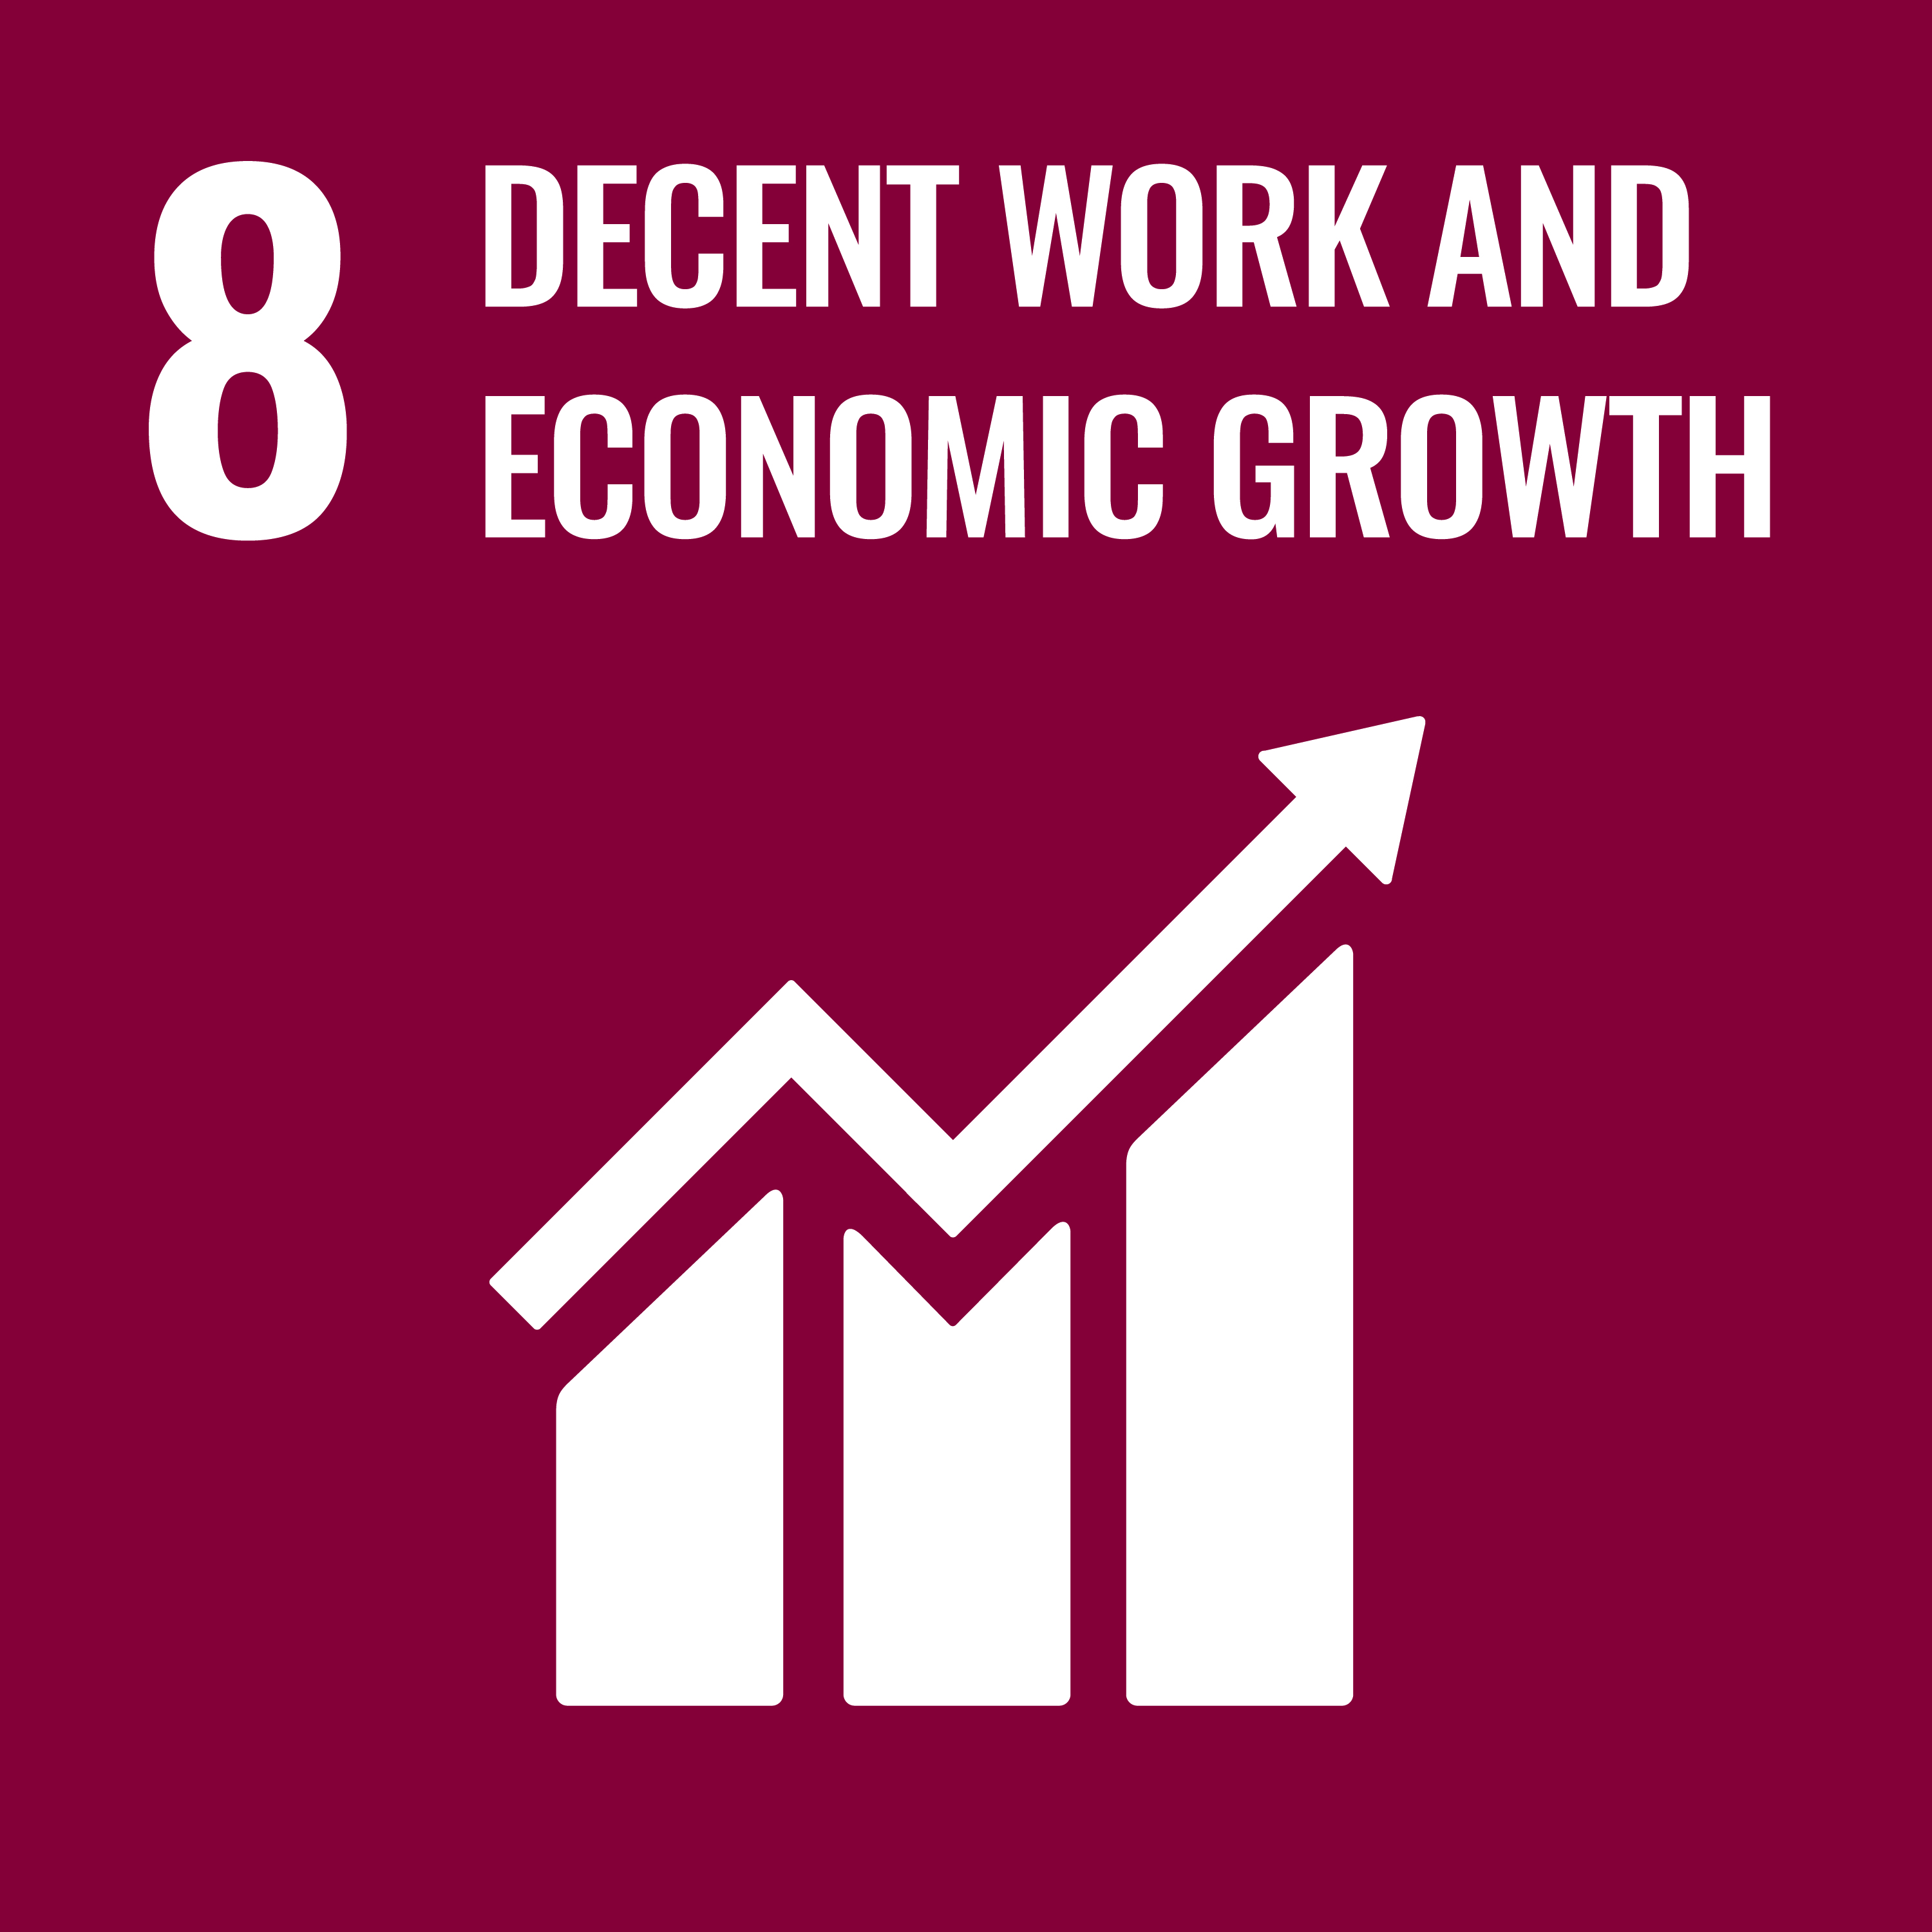
\includegraphics[width=\linewidth]{Pictures/ODD/ODD08.jpg}
	\end{minipage}
	\hfill
	\begin{minipage}{0.8\textwidth}
		{\bfseries\Large ODD 8 : }\\[2pt]
		\textit{Promouvoir une croissance économique soutenue, partagée et durable, le plein emploi productif et un travail décent pour tous.}
	\end{minipage}
\end{simplebox2}



\section{Cible 8.5 : Travail décent et réduction du chômage}


La cible 8.5 vise à parvenir à un niveau d'emploi plein et productif et à garantir un travail décent pour tous, y compris les jeunes et les personnes handicapées, tout en assurant l'égalité de rémunération pour un travail de valeur égale.\\
Ce graphe montre l'évolution du taux de chômage de 2000 à 2025 au Sénégal

\begin{figure}[H]
	\centering
	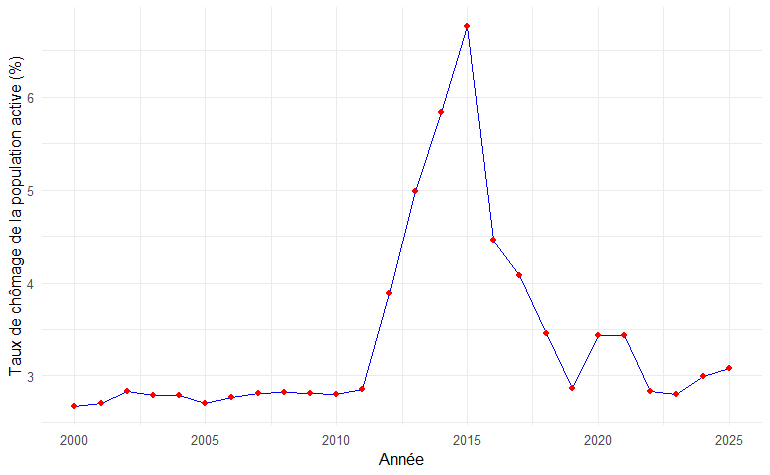
\includegraphics[width=0.8\textwidth]{Pictures/graphs/sdg8_unemp.png}
	\caption{Évolution du taux de chômage de la population active (15 ans et plus) au Sénégal}
	\label{fig:sdg8_5}
\end{figure}

 
 
On observe une hausse notable du chômage entre 2012 et 2015, avec un taux passant de 2,85\,\% à 6,76\,\%, suivie d'une diminution progressive pour atteindre environ 3\,\% dans les années récentes. 

Ces variations reflètent plusieurs facteurs possibles : des chocs économiques ou sectoriels, l'évolution du marché du travail, ainsi que l'entrée de jeunes sur le marché de l'emploi. 
Bien que les taux restent relativement bas, les hausses ponctuelles soulignent l'importance de politiques publiques visant à promouvoir un emploi décent et stable pour tous les segments de la population.

\section*{Synthèse de la performance - ODD8}

\begin{figure}[H]
	\centering
	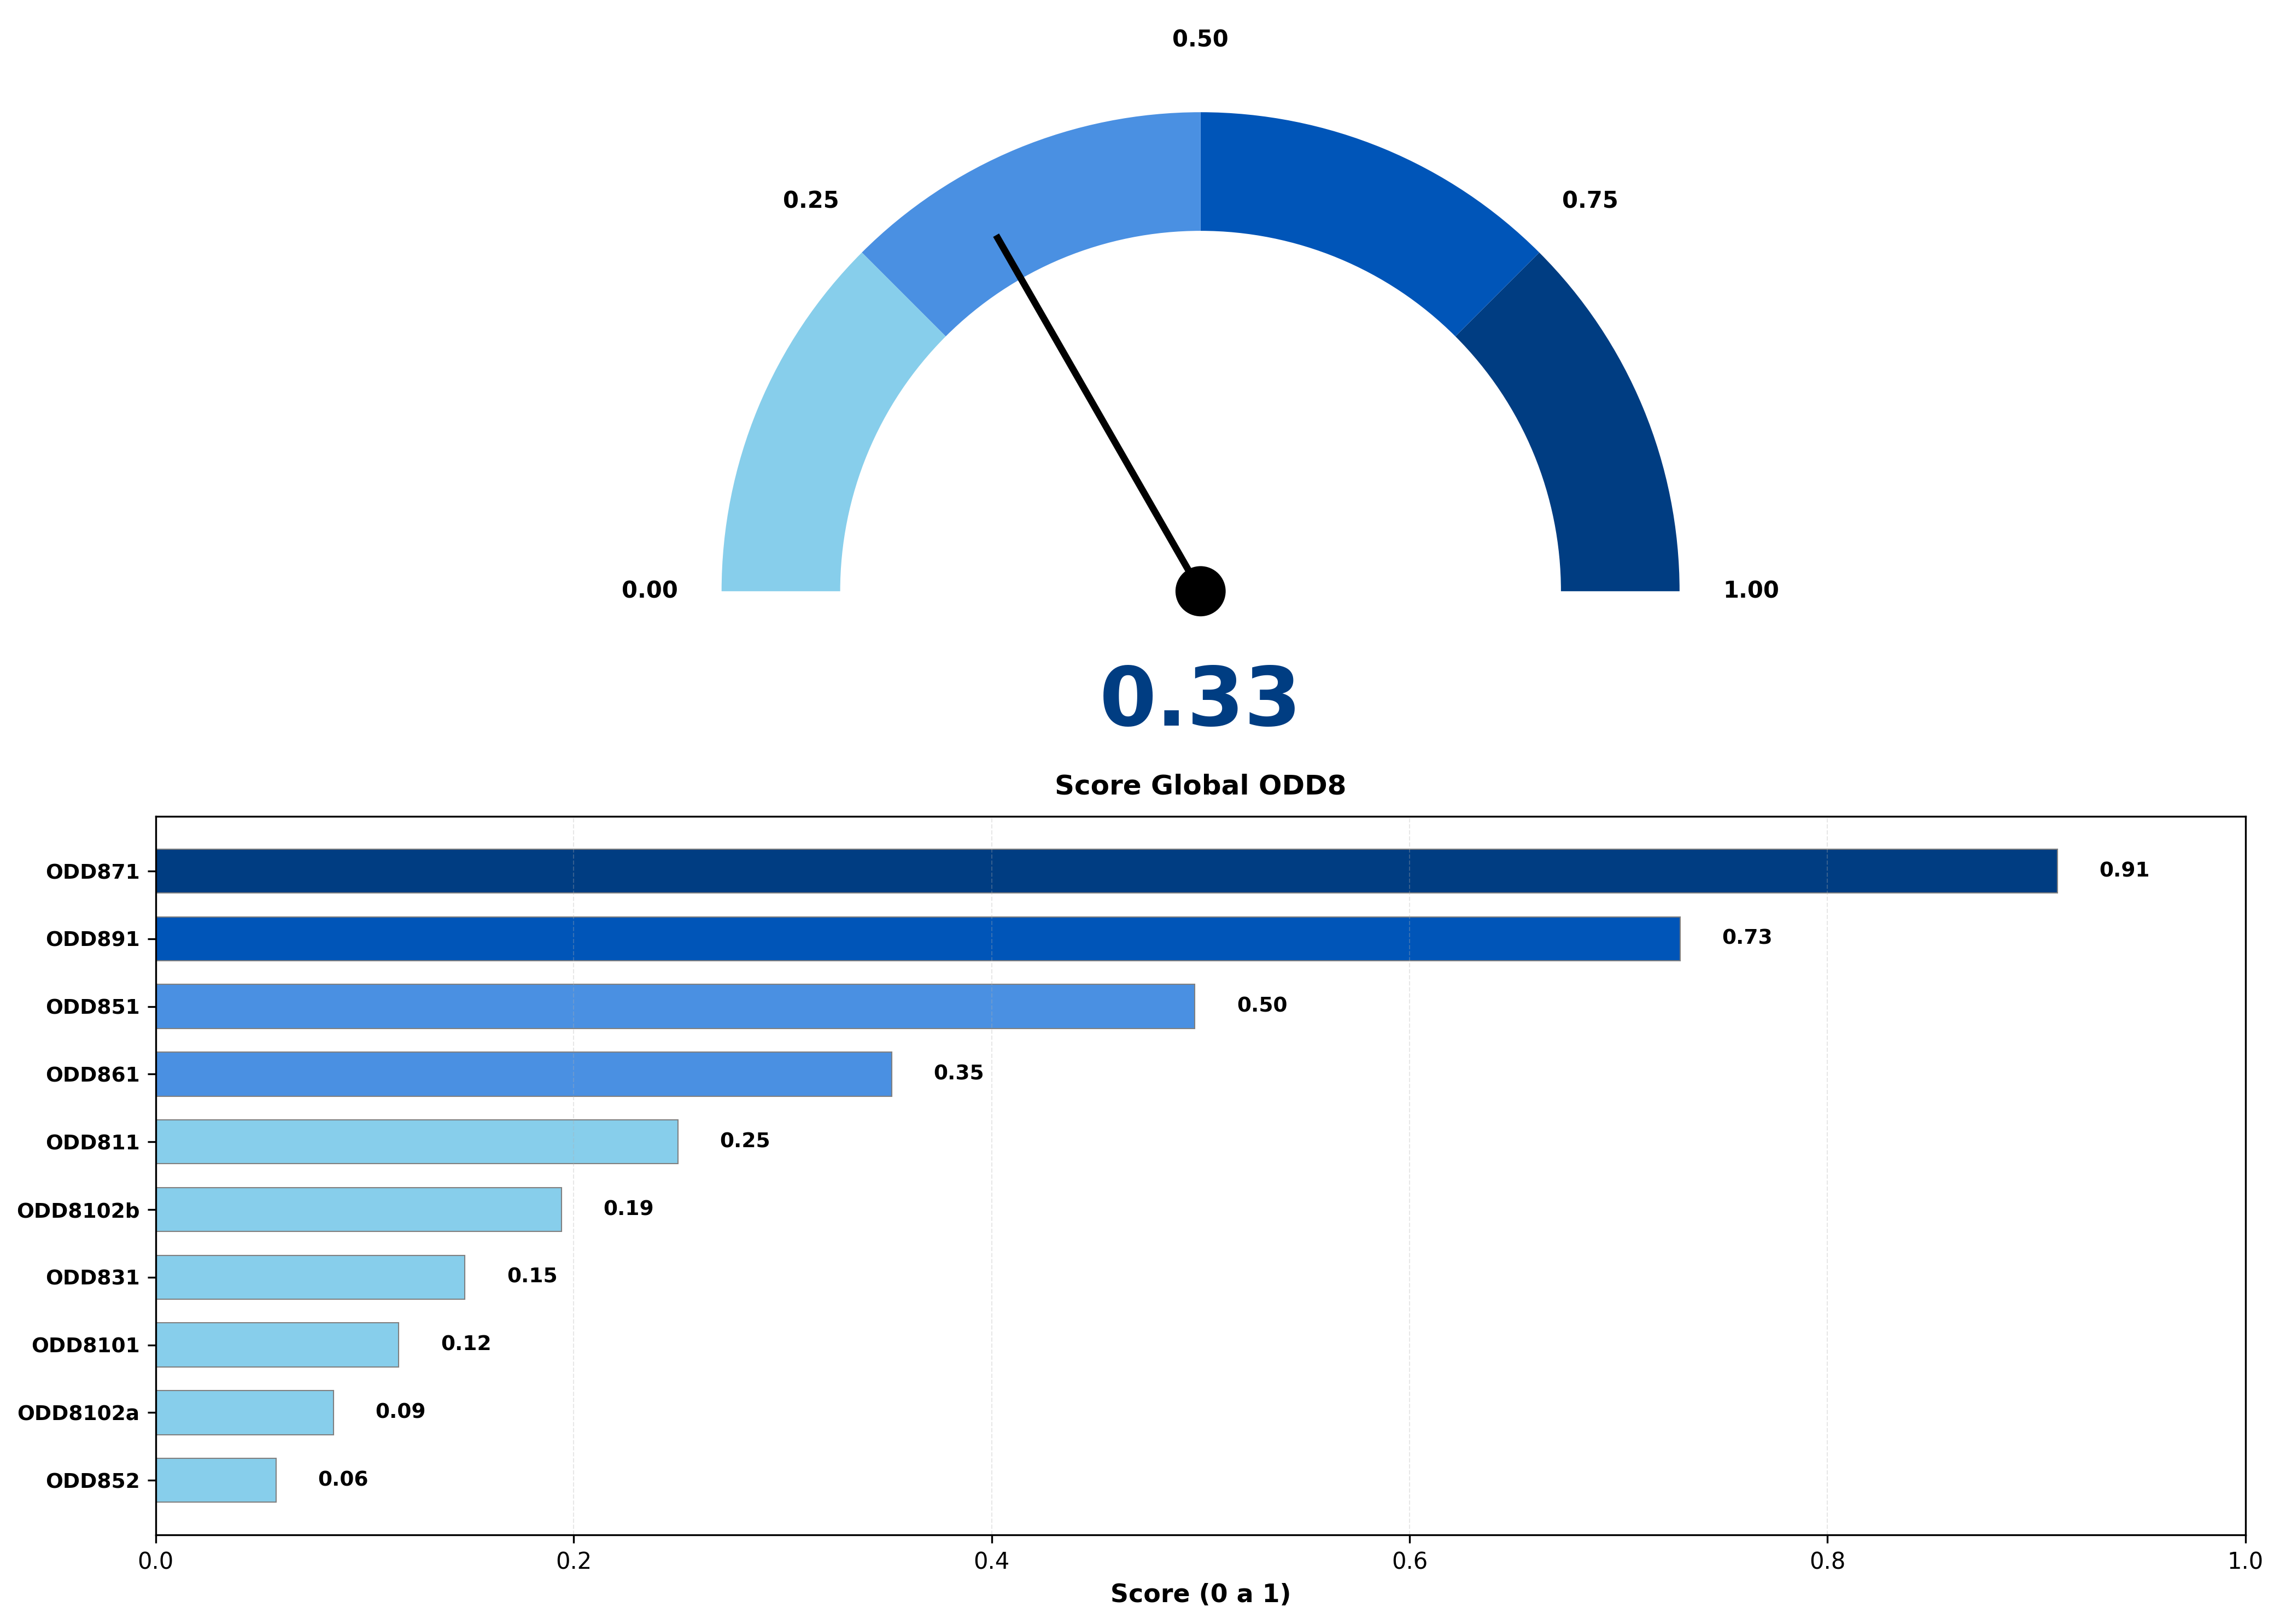
\includegraphics[width=0.95\textwidth]{Pictures/graphs/ODD8_scores.png}
	\caption{Performance par indicateur - ODD8}
\end{figure}

\begin{table}[H]
	\centering
	\begin{tabularx}{\textwidth}{l l c c c}
		\rowcolor[HTML]{003D82}
		\color{white}\textbf{Code} & \color{white}\textbf{Indicateur} & \color{white}\textbf{Valeur} & \color{white}\textbf{Cible} & \color{white}\textbf{Score} \\
		\rowcolor[HTML]{F5F8FC}
		ODD852 & Taux d'emploi (\%) & 0.52 & 0.78 & 0.06 \\
		\rowcolor[HTML]{E8F0FF}
		ODD8102a & Possession de compte bancaire parmi les femmes & 0.09 & 1.00 & 0.09 \\
		\rowcolor[HTML]{F5F8FC}
		ODD8101 & Succursales et banques commerciales & 7.10 & 50.00 & 0.12 \\
		\rowcolor[HTML]{E8F0FF}
		ODD831 & Emploi informel dans les secteurs non agricoles  & 0.93 & 0.50 & 0.15 \\
		\rowcolor[HTML]{F5F8FC}
		ODD8102b & Possession de compte bancaire parmi les hommes & 0.19 & 1.00 & 0.19 \\
		\rowcolor[HTML]{E8F0FF}
		ODD811 & Taux de croissance du PIB & 0.01 & 0.04 & 0.25 \\
		\rowcolor[HTML]{F5F8FC}
		ODD861 & NEET & 0.47 & 0.81 & 0.35 \\
		\rowcolor[HTML]{E8F0FF}
		ODD851 & Rémunération horaire moyenne des salariés & 833.60 & 1676.37 & 0.50 \\
		\rowcolor[HTML]{F5F8FC}
		ODD891 & PIB directement tiré du tourisme, en proportion du PIB total & 0.01 & 0.01 & 0.73 \\
		\rowcolor[HTML]{E8F0FF}
		ODD871 & Enfants âgés de 5 à 15 ans qui travaillent & 0.04 & 0.00 & 0.91 \\
	\end{tabularx}
\end{table}

L'analyse du ODD8 révèle un score global de 0.3340, basé sur 10 indicateur(s). Les performances varient de 0.06 à 0.91, montrant une certaine disparité dans la mise en oeuvre des cibles. Les indicateurs critiques (score < 0,30) nécessitent une attention particulière.


%%%%%%%%%%%%%%%%%%%%% ODD9 %%%%%%%%%%%%%%%%%%%%%%%%%%%

\newpage
\begin{simplebox2}
	
	\begin{minipage}{0.15\textwidth}
		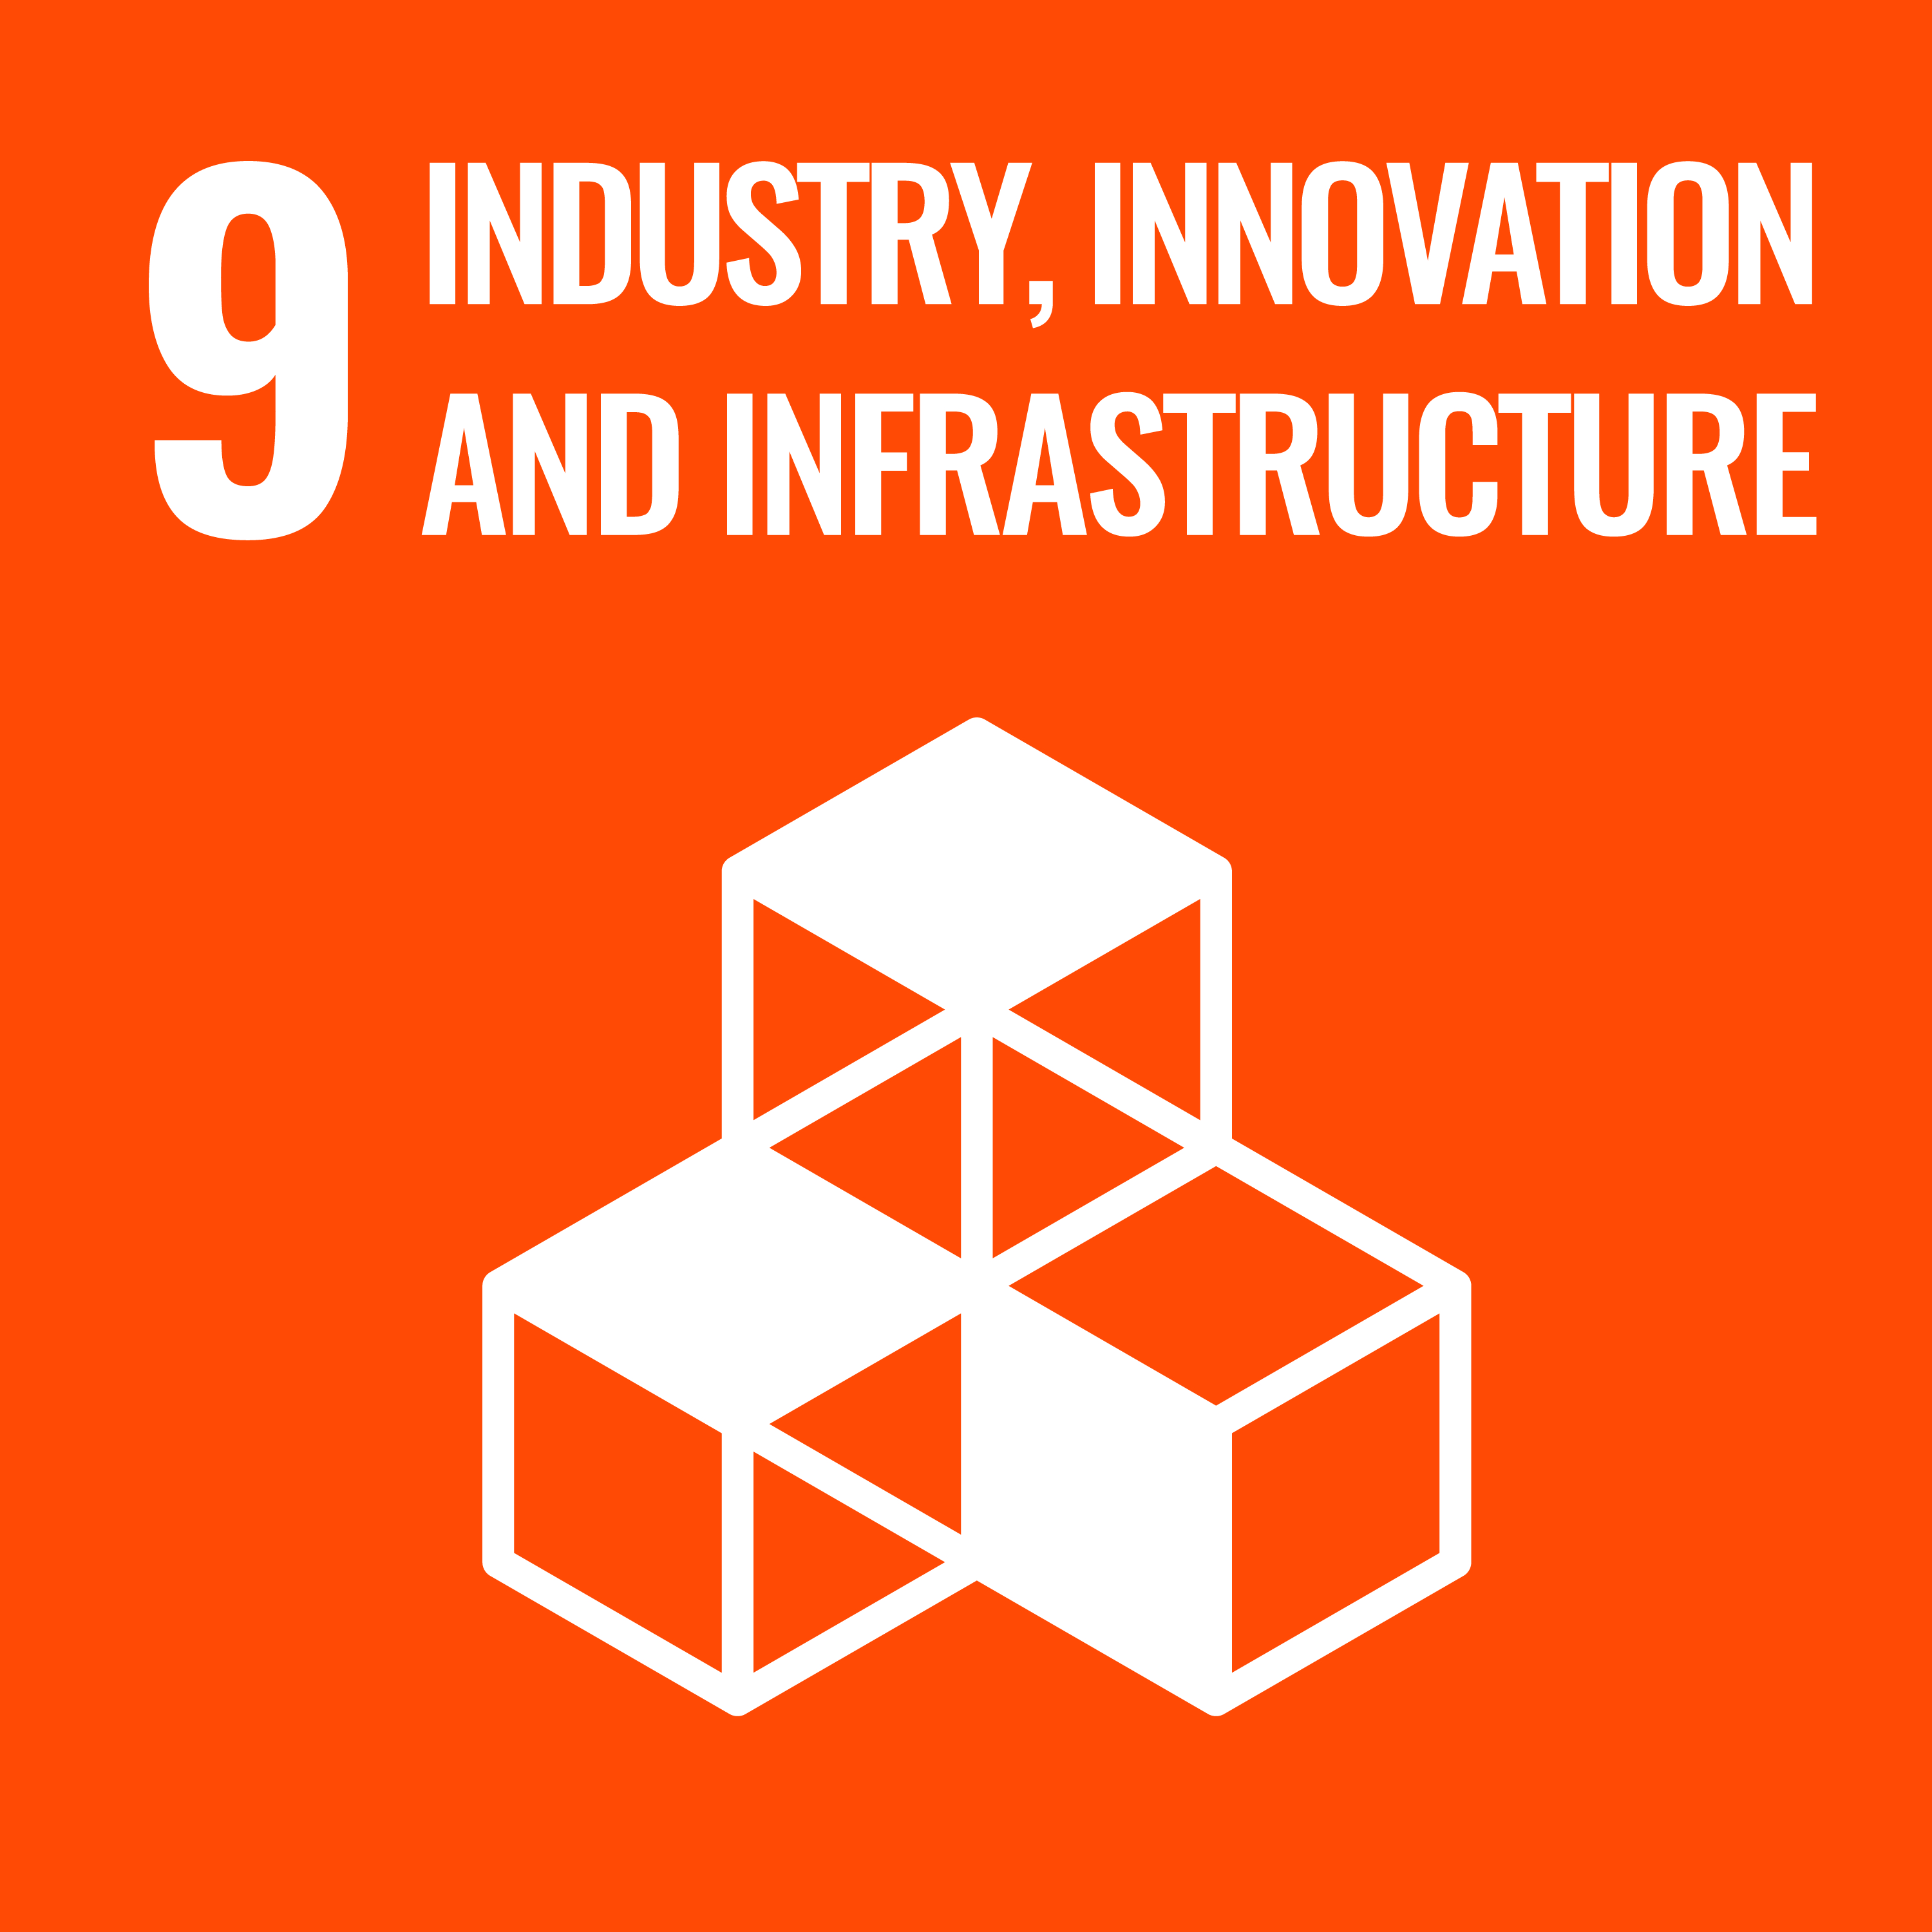
\includegraphics[width=\linewidth]{Pictures/ODD/ODD09.jpg}
	\end{minipage}
	\hfill
	\begin{minipage}{0.8\textwidth}
		{\bfseries\Large ODD 9 : }\\[2pt]
		\textit{Bâtir une infrastructure résiliente, promouvoir une industrialisation durable qui profite à tous et encourager l’innovation.}
	\end{minipage}
\end{simplebox2}



\section*{Cible 9.5 : Innovation et infrastructure scientifique}
La cible 9.5 vise à renforcer la recherche scientifique et technologique et à accroître le nombre de chercheurs et les dépenses en R\&D, afin de stimuler l'innovation et soutenir le développement industriel durable.

Les données sur l'accès à Internet et la production scientifique  au Sénégal montrent une évolution progressive depuis 2000. 
La part de la population utilisant Internet a augmenté de 0,40\,\% à 60,61\,\%, traduisant les efforts consentis pour développer les infrastructures numériques et améliorer l'accès à l'information. 
En parallèle, le nombre d'articles scientifiques publiés pour 1\,000 habitants est passé de 0,02 à 0,06, indiquant une croissance encore modeste mais continue de l'activité scientifique et de l'innovation dans le pays.

\begin{figure}[H]
	\centering
	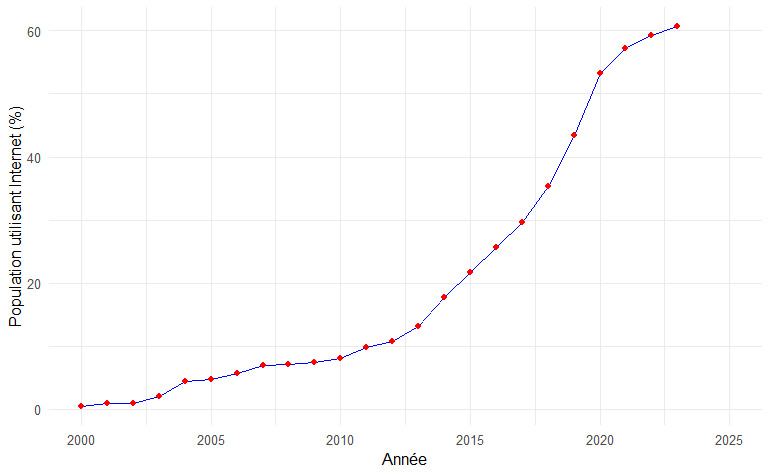
\includegraphics[width=0.8\textwidth]{Pictures/graphs/sdg9_intuse.png}
	\caption{Évolution de l'utilisation d'Internet au Sénégal}
	\label{fig:sdg9_intuse}
\end{figure}

\begin{figure}[H]
	\centering
	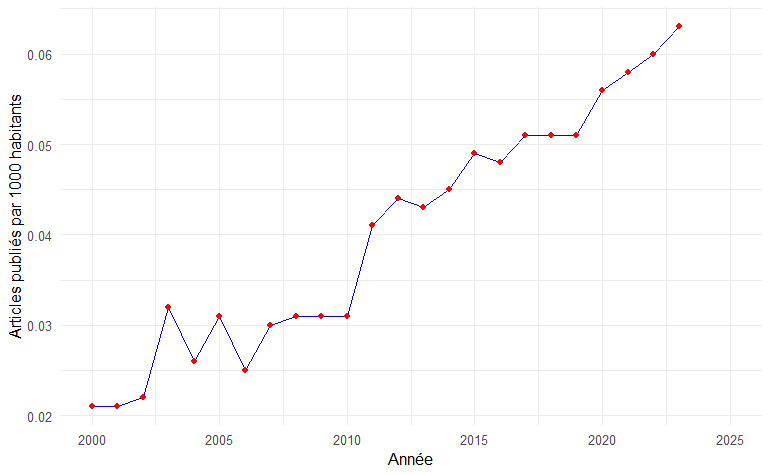
\includegraphics[width=0.8\textwidth]{Pictures/graphs/sdg9_articles.png}
	\caption{Évolution du nombre d'articles scientifiques publiés par 1\,000 habitants au Sénégal}
	\label{fig:sdg9_articles}
\end{figure}


\section*{Synthèse de la performance - ODD9}

\begin{figure}[H]
	\centering
	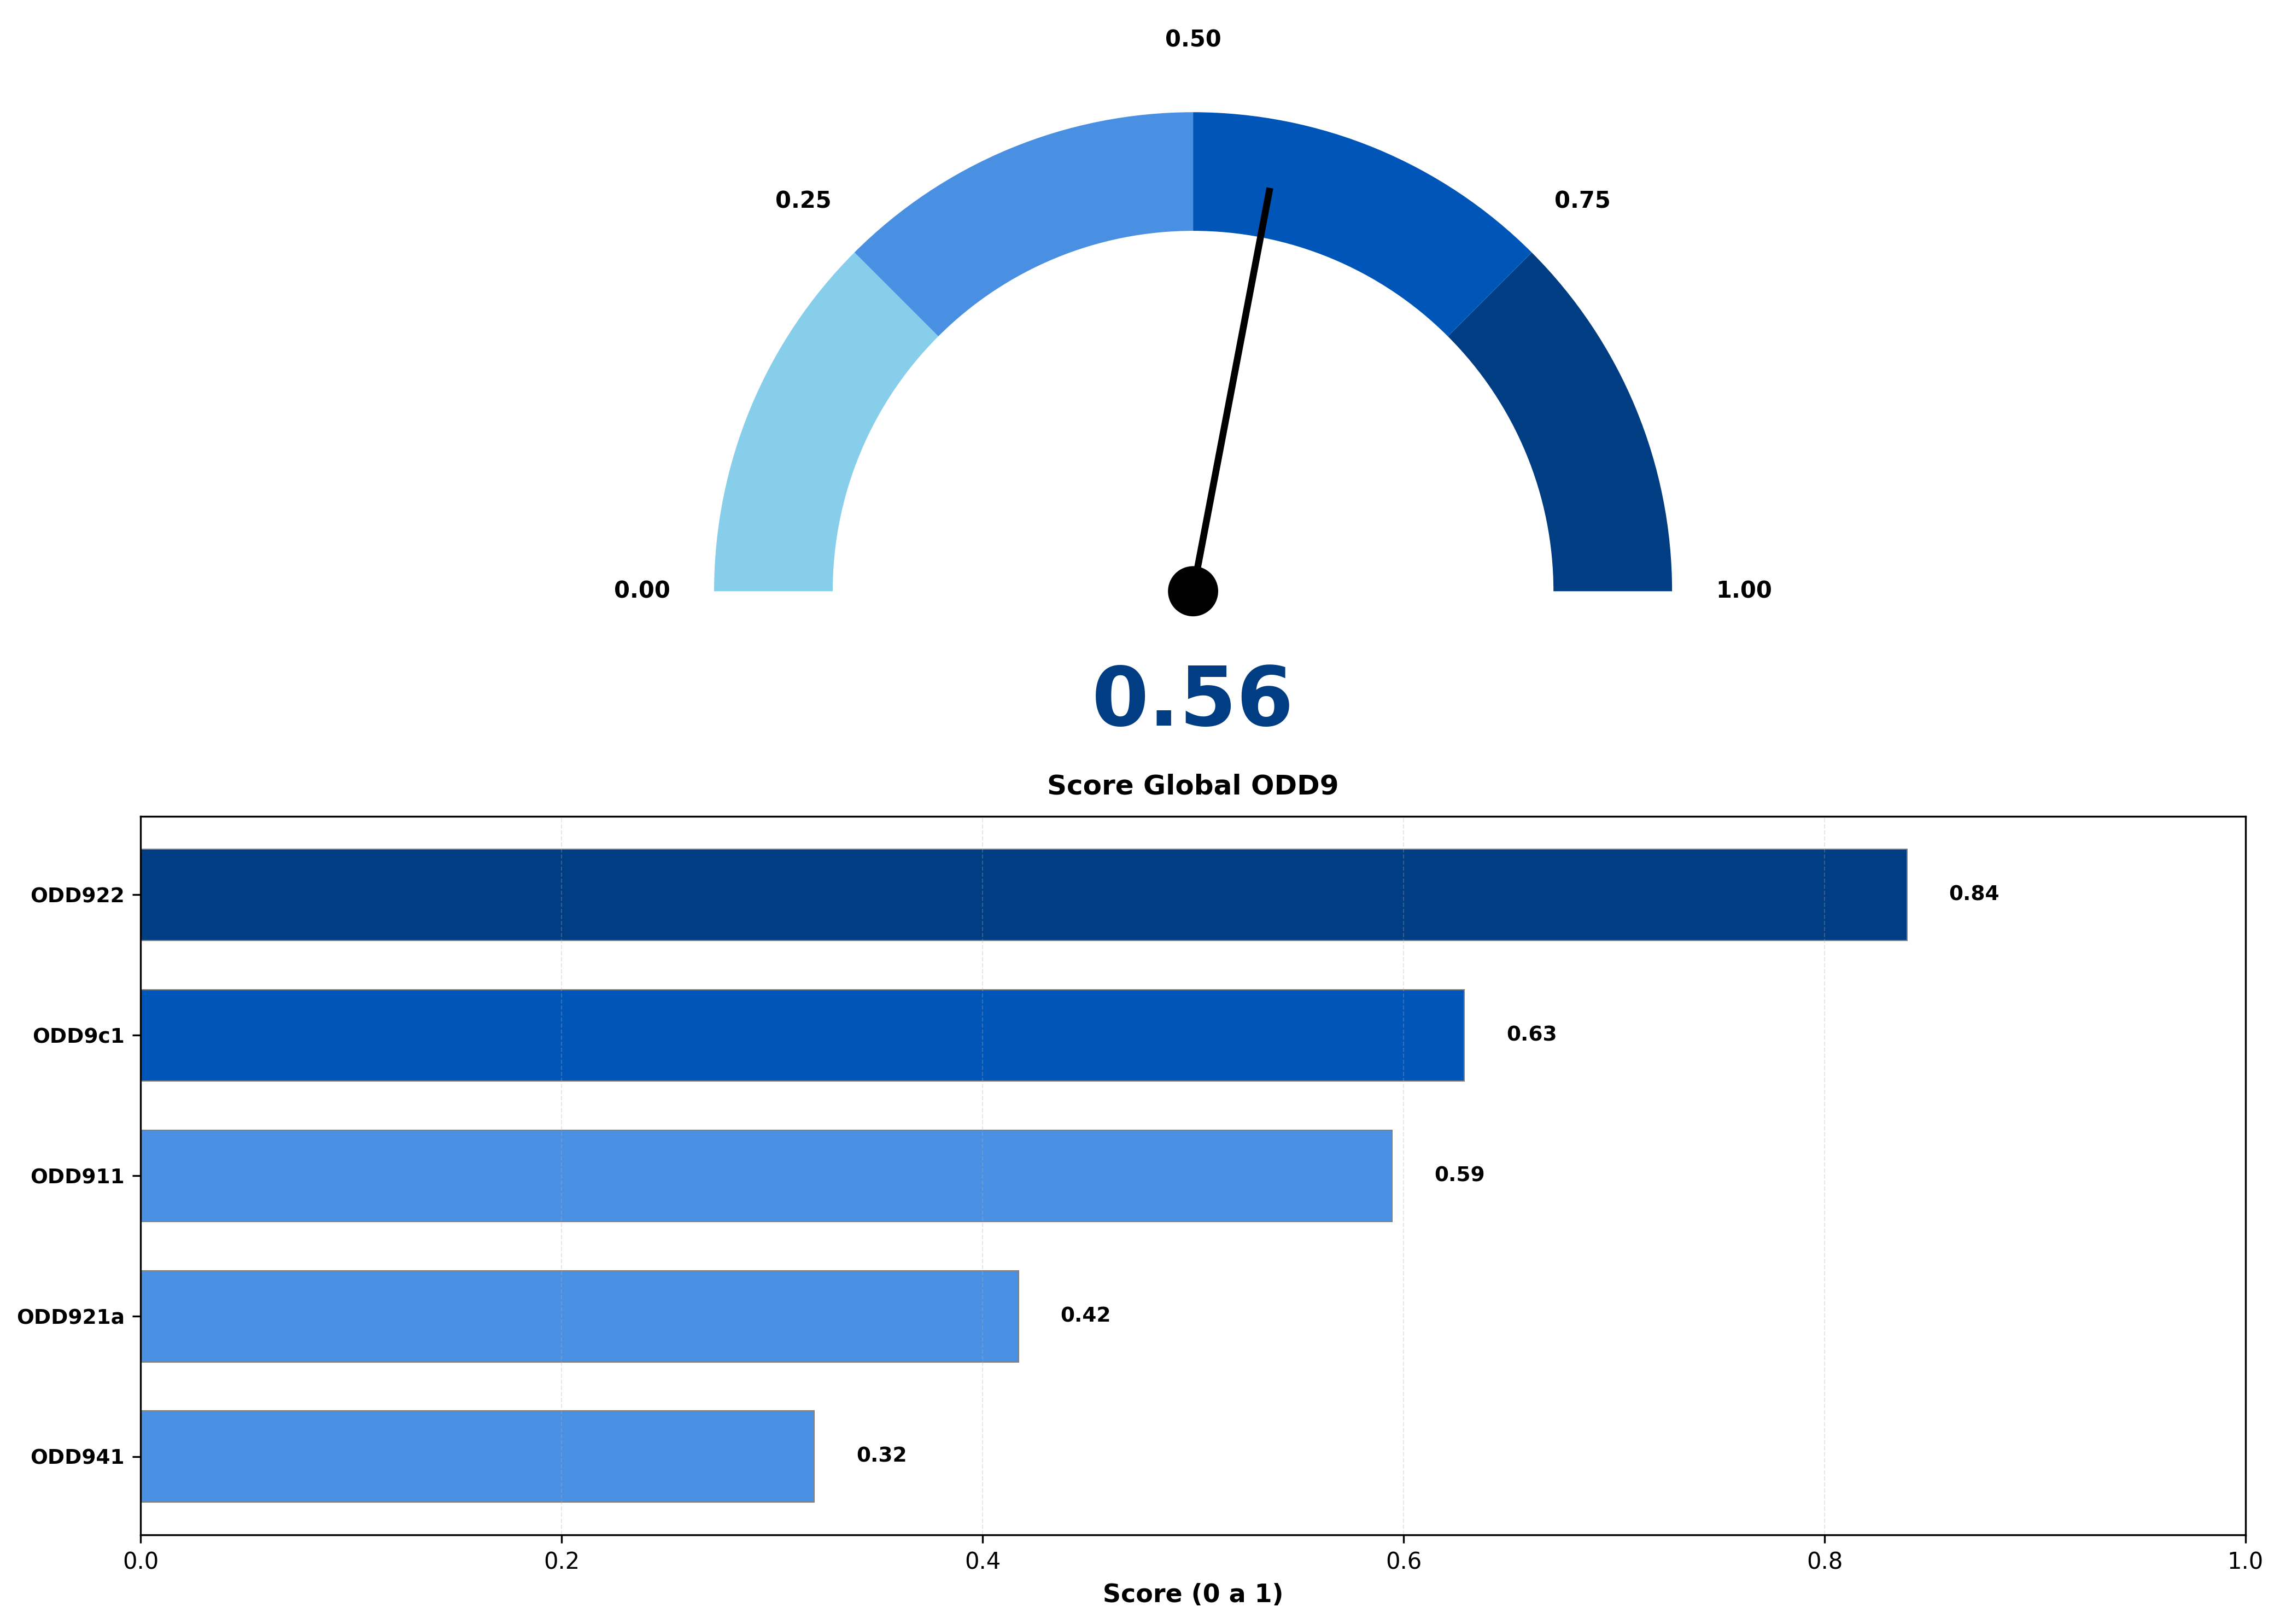
\includegraphics[width=0.95\textwidth]{Pictures/graphs/ODD9_scores.png}
	\caption{Performance par indicateur - ODD9}
\end{figure}

\begin{table}[H]
	\centering
	\begin{tabularx}{\textwidth}{l l c c c}
		\rowcolor[HTML]{003D82}
		\color{white}\textbf{Code} & \color{white}\textbf{Indicateur} & \color{white}\textbf{Valeur} & \color{white}\textbf{Cible} & \color{white}\textbf{Score} \\
		\rowcolor[HTML]{F5F8FC}
		ODD941 & Émissions de CO2 par unité de valeur ajoutée & 0.68 & 0.00 & 0.32 \\
		\rowcolor[HTML]{E8F0FF}
		ODD921a & VA dans la manufacture, en proportion du PIB  et par hbt & 0.14 & 0.34 & 0.42 \\
		\rowcolor[HTML]{F5F8FC}
		ODD911 & Moins de 2 km d'une route praticable à toute saison & 0.68 & 0.90 & 0.59 \\
		\rowcolor[HTML]{E8F0FF}
		ODD9c1 & Accés au réseau mobile & 0.64 & 1.00 & 0.63 \\
		\rowcolor[HTML]{F5F8FC}
		ODD922 & Emploi dans l'industrie manufacturière & 0.25 & 0.30 & 0.84 \\
	\end{tabularx}
\end{table}

L'analyse du ODD9 révèle un score global de 0.5599, basé sur 5 indicateur(s). Les performances varient de 0.32 à 0.84, montrant une certaine disparité dans la mise en oeuvre des cibles. Les indicateurs critiques (score < 0,30) nécessitent une attention particulière.

%%%%%%%%%%%%%%%%%%%%% ODD10 %%%%%%%%%%%%%%%%%%%%%%%%%%%

\newpage
\begin{simplebox2}
	
	\begin{minipage}{0.15\textwidth}
		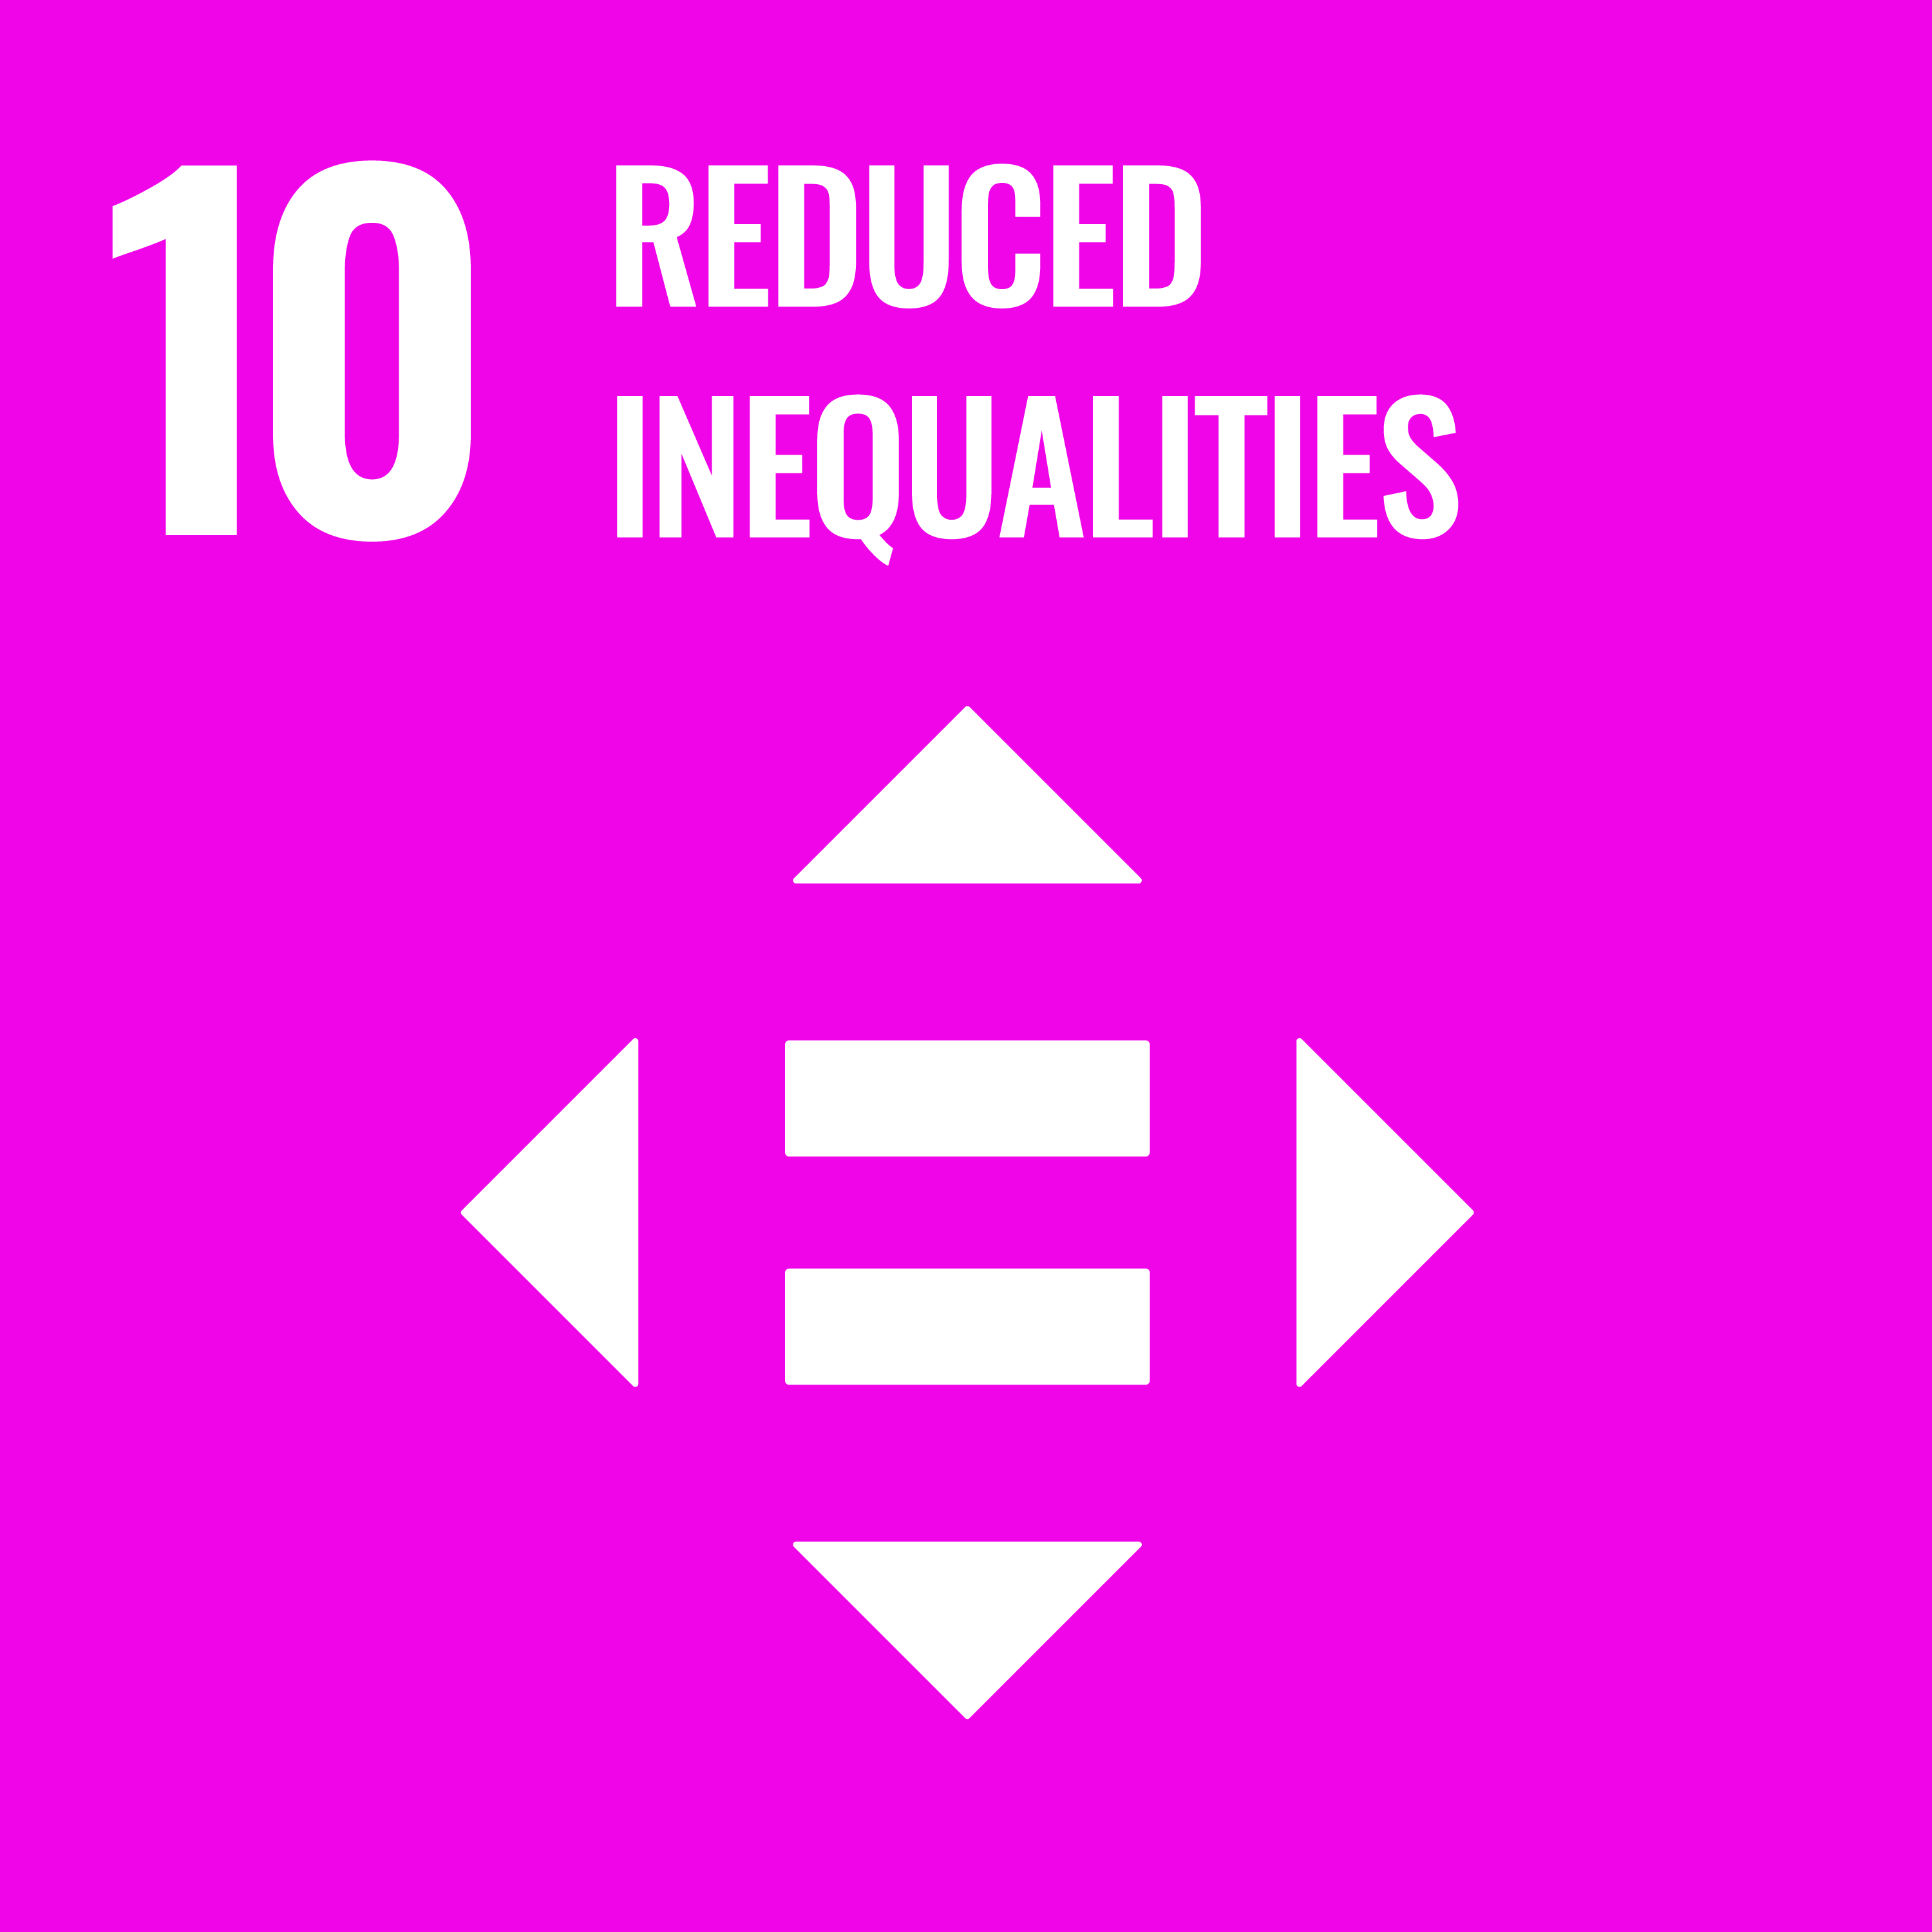
\includegraphics[width=\linewidth]{Pictures/ODD/ODD10.jpg}
	\end{minipage}
	\hfill
	\begin{minipage}{0.8\textwidth}
		{\bfseries\Large ODD 10 : }\\[2pt]
		\textit{Réduire les inégalités dans les pays et d’un pays à l’autre.}
	\end{minipage}
\end{simplebox2}


\section{Cible 10.1 : Réduction des inégalités de revenus}

La cible 10.1 vise à assurer, d’ici à 2030, une croissance inclusive en favorisant l’augmentation des revenus des 40\,\% les plus pauvres de la population à un rythme supérieur à la moyenne nationale. 
Elle a pour objectif de réduire durablement les inégalités de revenus au sein des pays.

\begin{table}[H]
	\centering
	\caption{Évolution des indicateurs d’inégalités de revenus au Sénégal}
	\label{tab:sdg10_ineq}
	\begin{tabular}{lcc}
		\hline
		\textbf{Année} & \textbf{Coefficient de Gini} & \textbf{Ratio de Palma} \\
		\hline
		2001 & 41,20 & 1,98 \\
		2005 & 39,20 & 1,78 \\
		2011 & 40,30 & 1,89 \\
		2018 & 38,30 & 1,72 \\
		2021 & 36,20 & 1,53 \\
		\hline
	\end{tabular}
\end{table}

Les résultats présentés dans le tableau~\ref{tab:sdg10_ineq} indiquent une tendance globale à la réduction des inégalités de revenus au Sénégal sur la période étudiée. 
Le coefficient de Gini diminue progressivement, passant de 41,20 en 2001 à 36,20 en 2021, ce qui traduit une réduction relative des écarts de revenus entre les ménages.

Cette évolution est confirmée par le ratio de Palma, qui mesure le rapport entre les revenus des 10\,\% les plus riches et ceux des 40\,\% les plus pauvres. 
La baisse de cet indicateur, de 1,98 à 1,53, suggère une diminution de la concentration des revenus au profit des populations les plus modestes.

Malgré ces progrès, les niveaux d’inégalités demeurent significatifs, ce qui souligne la nécessité de poursuivre et de renforcer les politiques publiques visant à promouvoir une croissance plus équitable et inclusive, conformément aux objectifs de l’ODD~10.

\section*{Synthèse de la performance - ODD10}

\begin{figure}[H]
	\centering
	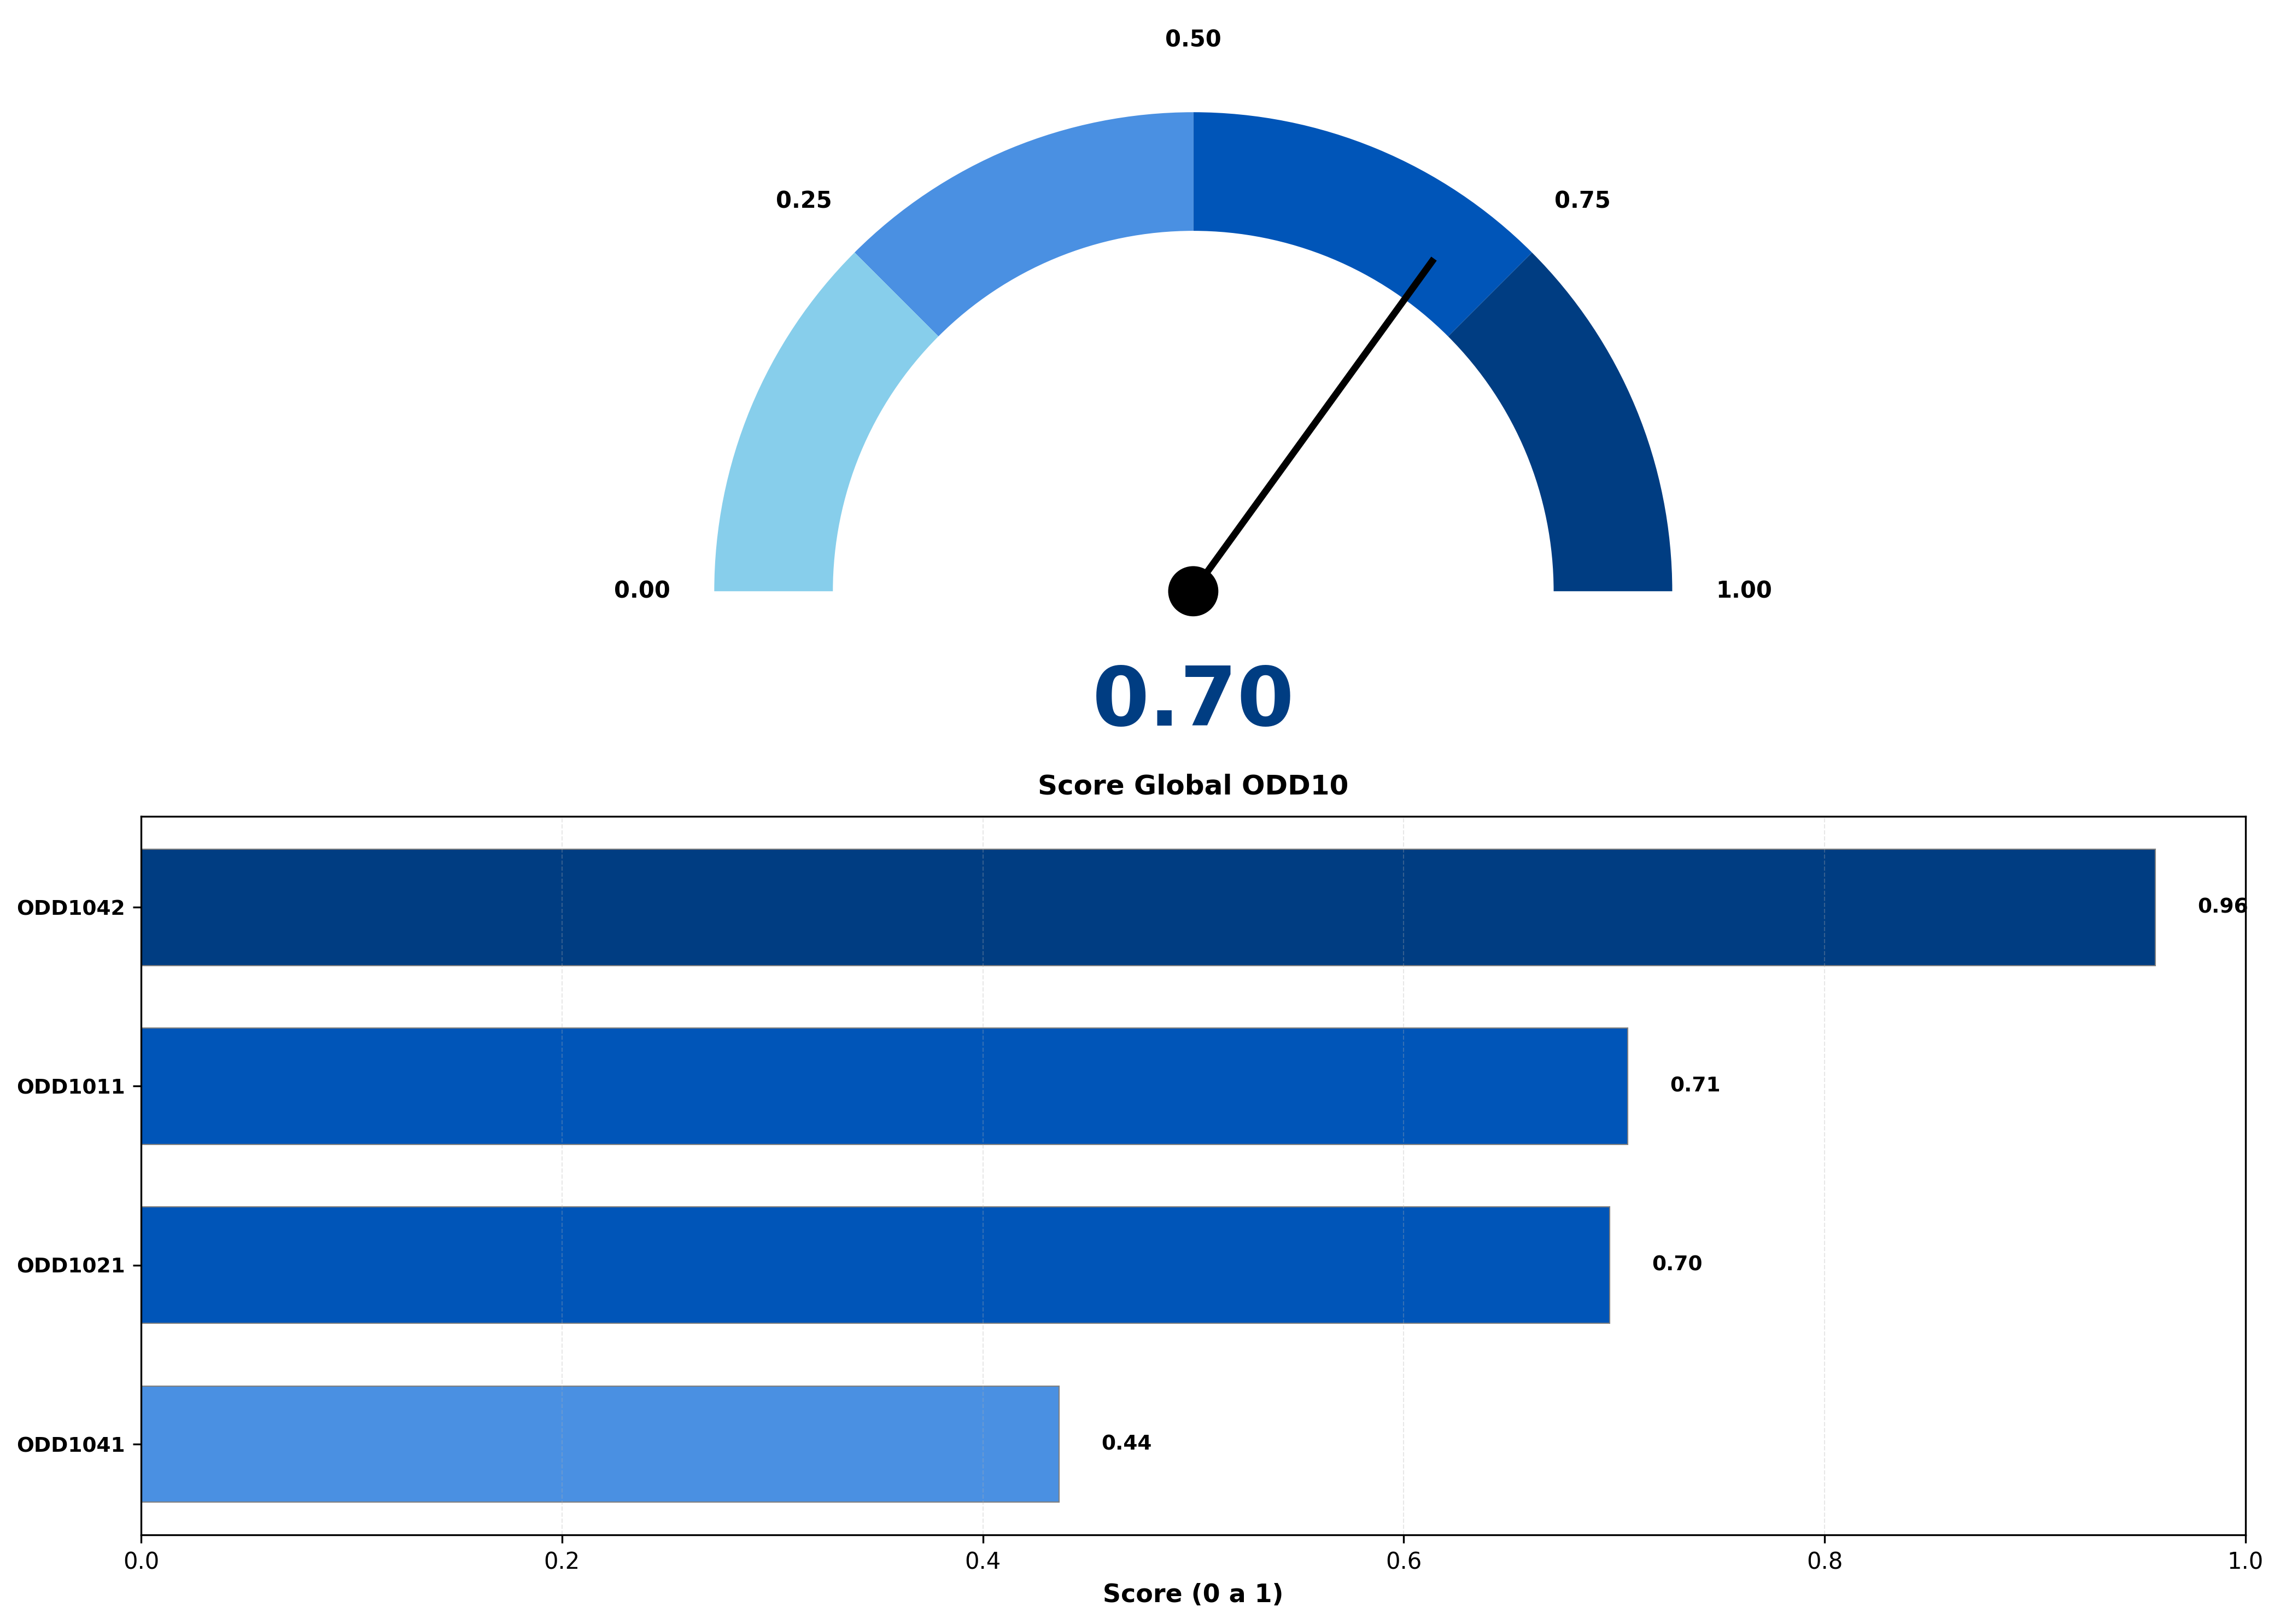
\includegraphics[width=0.95\textwidth]{Pictures/graphs/ODD10_scores.png}
	\caption{Performance par indicateur - ODD10}
\end{figure}

\begin{table}[H]
	\centering
	\begin{tabularx}{\textwidth}{l l c c c}
		\rowcolor[HTML]{003D82}
		\color{white}\textbf{Code} & \color{white}\textbf{Indicateur} & \color{white}\textbf{Valeur} & \color{white}\textbf{Cible} & \color{white}\textbf{Score} \\
		\rowcolor[HTML]{F5F8FC}
		ODD1041 & Part du travail dans le PIB & 0.24 & 0.55 & 0.44 \\
		\rowcolor[HTML]{E8F0FF}
		ODD1021 & Revenu inférieur à la moitié du revenu median & 0.10 & 0.15 & 0.70 \\
		\rowcolor[HTML]{F5F8FC}
		ODD1011 & Dépenses des 40 \% de la population les plus pauvre & 0.28 & 0.40 & 0.71 \\
		\rowcolor[HTML]{E8F0FF}
		ODD1042 & Indice de Gini & 0.33 & 0.30 & 0.96 \\
	\end{tabularx}
\end{table}

L'analyse du ODD10 révèle un score global de 0.6994, basé sur 4 indicateur(s). Les performances varient de 0.44 à 0.96, montrant une certaine disparité dans la mise en oeuvre des cibles. Les indicateurs critiques (score < 0,30) nécessitent une attention particulière.


%%%%%%%%%%%%%%%%%%%%% ODD11 %%%%%%%%%%%%%%%%%%%%%%%%%%%

\newpage
\begin{simplebox2}
	
	\begin{minipage}{0.15\textwidth}
		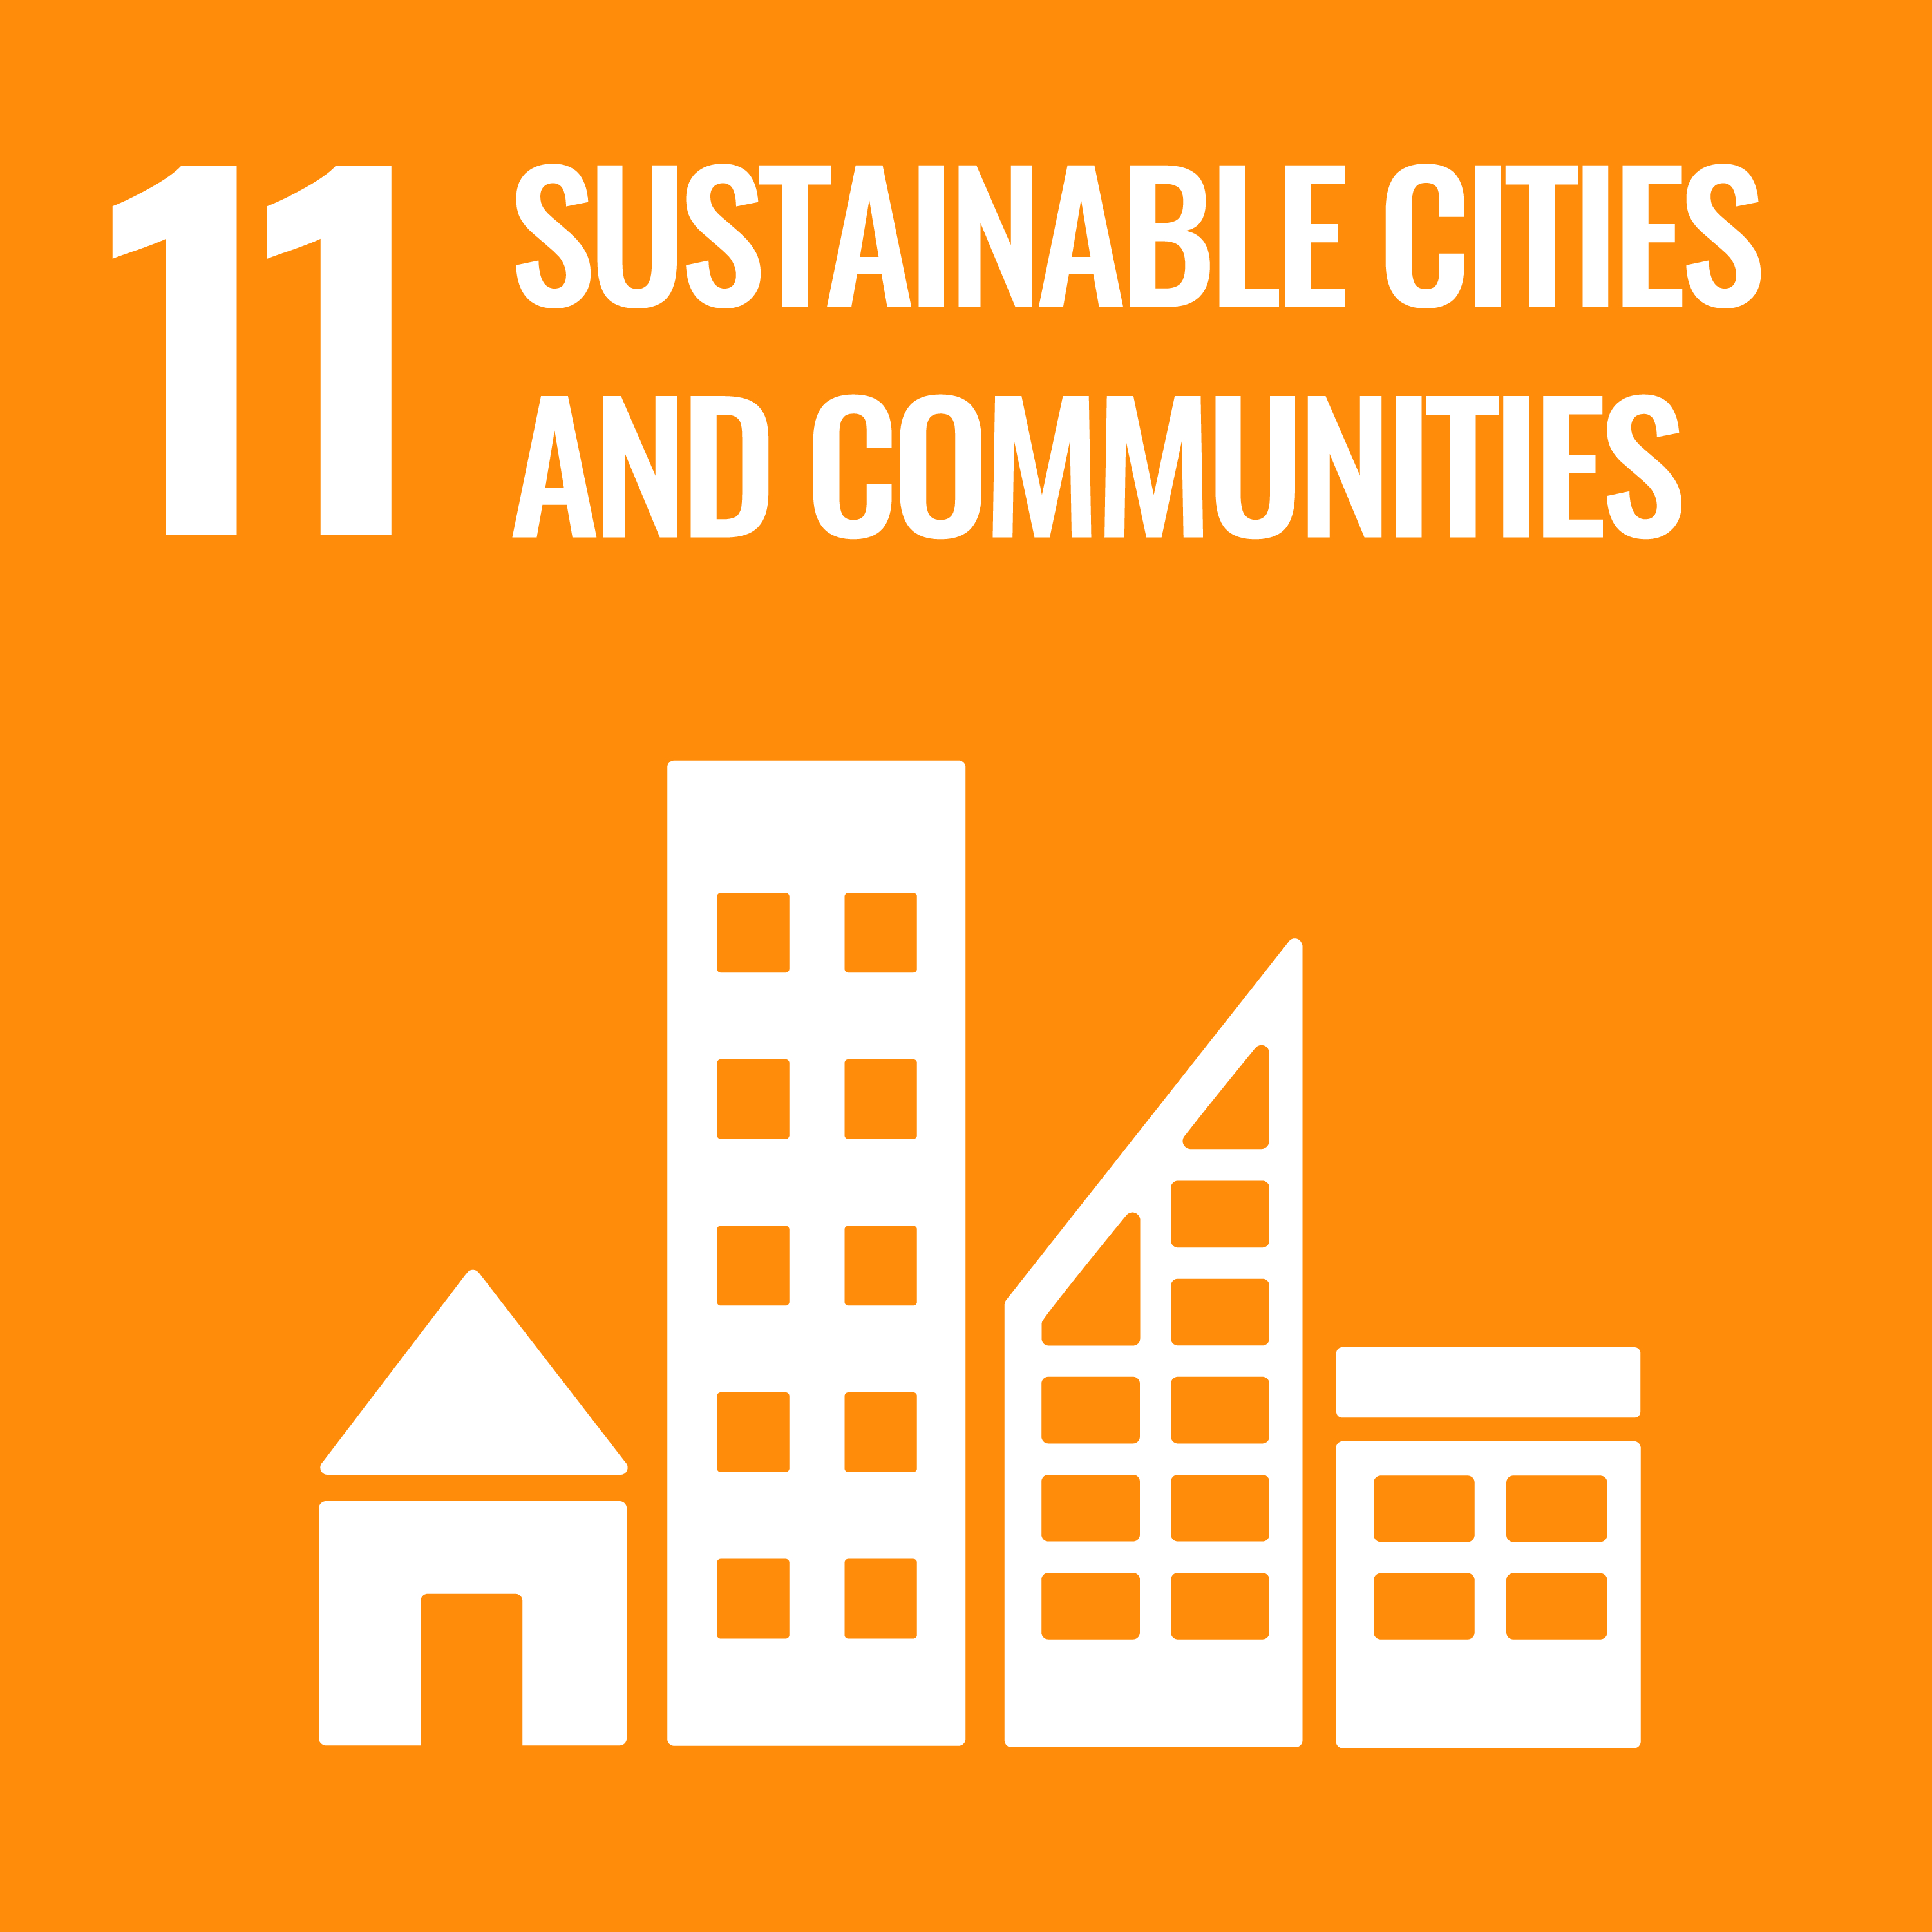
\includegraphics[width=\linewidth]{Pictures/ODD/ODD11.jpg}
	\end{minipage}
	\hfill
	\begin{minipage}{0.8\textwidth}
		{\bfseries\Large ODD 11 : }\\[2pt]
		\textit{Faire en sorte que les villes et les établissements humains soient ouverts à tous, sûrs, résilients et durables.}
	\end{minipage}
\end{simplebox2}


\section{ODD 11 : Villes et communautés durables}

L’Objectif de Développement Durable 11 vise à faire en sorte que les villes et les établissements humains soient inclusifs, sûrs, résilients et durables. Plusieurs cibles de cet objectif peuvent être analysées à partir des indicateurs disponibles pour le Sénégal, notamment la cible 11.1 relative à l’amélioration des conditions de logement, la cible 11.6 portant sur la réduction de l’impact environnemental des villes, ainsi que l’accès aux services urbains de base.

Les données montrent tout d’abord une baisse progressive de la proportion de la population urbaine vivant dans des quartiers précaires, passant d’environ 67\,\% au début de la période à près de 31\,\%, avant d’enregistrer une remontée récente autour de 46\,\%. Cette évolution traduit des efforts réels en matière de politiques de logement et d’aménagement urbain, mais met également en évidence la persistance de vulnérabilités structurelles liées à l’urbanisation rapide, à la pression démographique et à l’insuffisance de logements formels accessibles. Ainsi, malgré les progrès observés, l’objectif d’un accès universel à un logement adéquat reste encore éloigné.

En ce qui concerne la cible 11.6, les niveaux de concentration annuelle moyenne des particules fines PM$_{2.5}$ demeurent élevés et relativement volatils, oscillant entre environ 35 et 48~$\mu$g/m$^3$, des valeurs nettement supérieures aux seuils recommandés par l’Organisation mondiale de la santé. Cette situation souligne les défis persistants en matière de pollution atmosphérique urbaine, liés notamment au trafic routier, à l’utilisation de combustibles polluants et à une gestion encore insuffisante des déchets urbains.

Par ailleurs, l’accès à l’eau potable par canalisation en milieu urbain connaît une amélioration continue, dépassant progressivement 87\,\% de la population urbaine. Cette évolution reflète des investissements soutenus dans les infrastructures de base et constitue un signal positif pour la durabilité des villes sénégalaises.

Globalement, le Sénégal a enregistré des avancées notables vers l’atteinte de l’ODD~11, en particulier en matière d’accès aux services urbains essentiels. Toutefois, des défis importants subsistent, notamment en ce qui concerne la réduction durable de l’habitat précaire et l’amélioration de la qualité de l’air. Ces résultats indiquent que, bien que la trajectoire soit globalement positive, des efforts supplémentaires et mieux ciblés demeurent nécessaires pour atteindre pleinement les objectifs fixés à l’horizon 2030.


%\newpage
%L’Objectif de Développement Durable 11 vise à rendre les villes et les établissements humains inclusifs, sûrs, résilients et durables. L’analyse s’appuie sur des indicateurs permettant d’évaluer les conditions de logement, la qualité de l’environnement urbain et l’accès aux services de base.
%
%\section{Cible 11.1 : Accès à un logement adéquat et amélioration des quartiers précaires}
%
%La cible 11.1 vise à garantir l’accès de tous à un logement adéquat, sûr et abordable, ainsi qu’à améliorer les quartiers de taudis. Elle est illustrée par la proportion de la population urbaine vivant dans des quartiers précaires (sdg11\_slums).
%
%\begin{figure}[H]
%	\centering
%	\includegraphics[width=0.75\textwidth]{figures/sdg11_slums.png}
%	\caption{Évolution de la proportion de la population urbaine vivant dans des quartiers précaires}
%	\label{fig:od11_slums}
%\end{figure}
%
%La figure \ref{fig:od11_slums} met en évidence une baisse progressive de la proportion de la population urbaine vivant dans des quartiers précaires. Cette évolution traduit des améliorations dans les politiques de logement et d’aménagement urbain, bien que le niveau reste encore élevé, indiquant la persistance de défis structurels en matière d’habitat.
%
%\section{Cible 11.6 : Qualité de l’air en milieu urbain}
%
%La cible 11.6 vise à réduire l’impact environnemental négatif des villes, notamment en améliorant la qualité de l’air. L’indicateur retenu est la concentration annuelle moyenne de particules fines PM2.5 (sdg11\_pm25).
%
%\begin{figure}[H]
%	\centering
%	\includegraphics[width=0.75\textwidth]{figures/od11_pm25.png}
%	\caption{Évolution de la concentration annuelle moyenne de PM2.5 en milieu urbain}
%	\label{fig:od11_pm25}
%\end{figure}
%
%La figure \ref{fig:od11_pm25} montre des niveaux de pollution atmosphérique élevés et fluctuants au cours du temps. Malgré certaines améliorations ponctuelles, les concentrations demeurent supérieures aux seuils recommandés, soulignant l’importance de renforcer les politiques environnementales urbaines.
%
%\subsection{Accès aux services de base : eau potable}
%
%L’accès à l’eau potable constitue un élément central de la durabilité urbaine. Il est mesuré par la proportion de la population urbaine ayant accès à une source d’eau améliorée par canalisation (sdg11\_pipedwat).
%
%\begin{figure}[H]
%	\centering
%	\includegraphics[width=0.75\textwidth]{figures/od11_pipedwat.png}
%	\caption{Évolution de l’accès à une source d’eau potable améliorée en milieu urbain}
%	\label{fig:od11_pipedwat}
%\end{figure}
%
%La figure \ref{fig:od11_pipedwat} met en évidence une progression régulière de l’accès à l’eau potable en milieu urbain. Cette tendance positive reflète des investissements continus dans les infrastructures de base, contribuant à l’amélioration des conditions de vie et à la résilience des villes.
%
%\subsection*{Synthèse}
%
%Dans l’ensemble, l’ODD 11 révèle des avancées notables en matière de logement et d’accès aux services essentiels. Toutefois, la persistance de la pollution de l’air et la proportion encore importante de population vivant dans des quartiers précaires soulignent la nécessité de politiques urbaines plus durables et intégrées.


\section*{Synthèse de la performance - ODD11}

\begin{figure}[H]
	\centering
	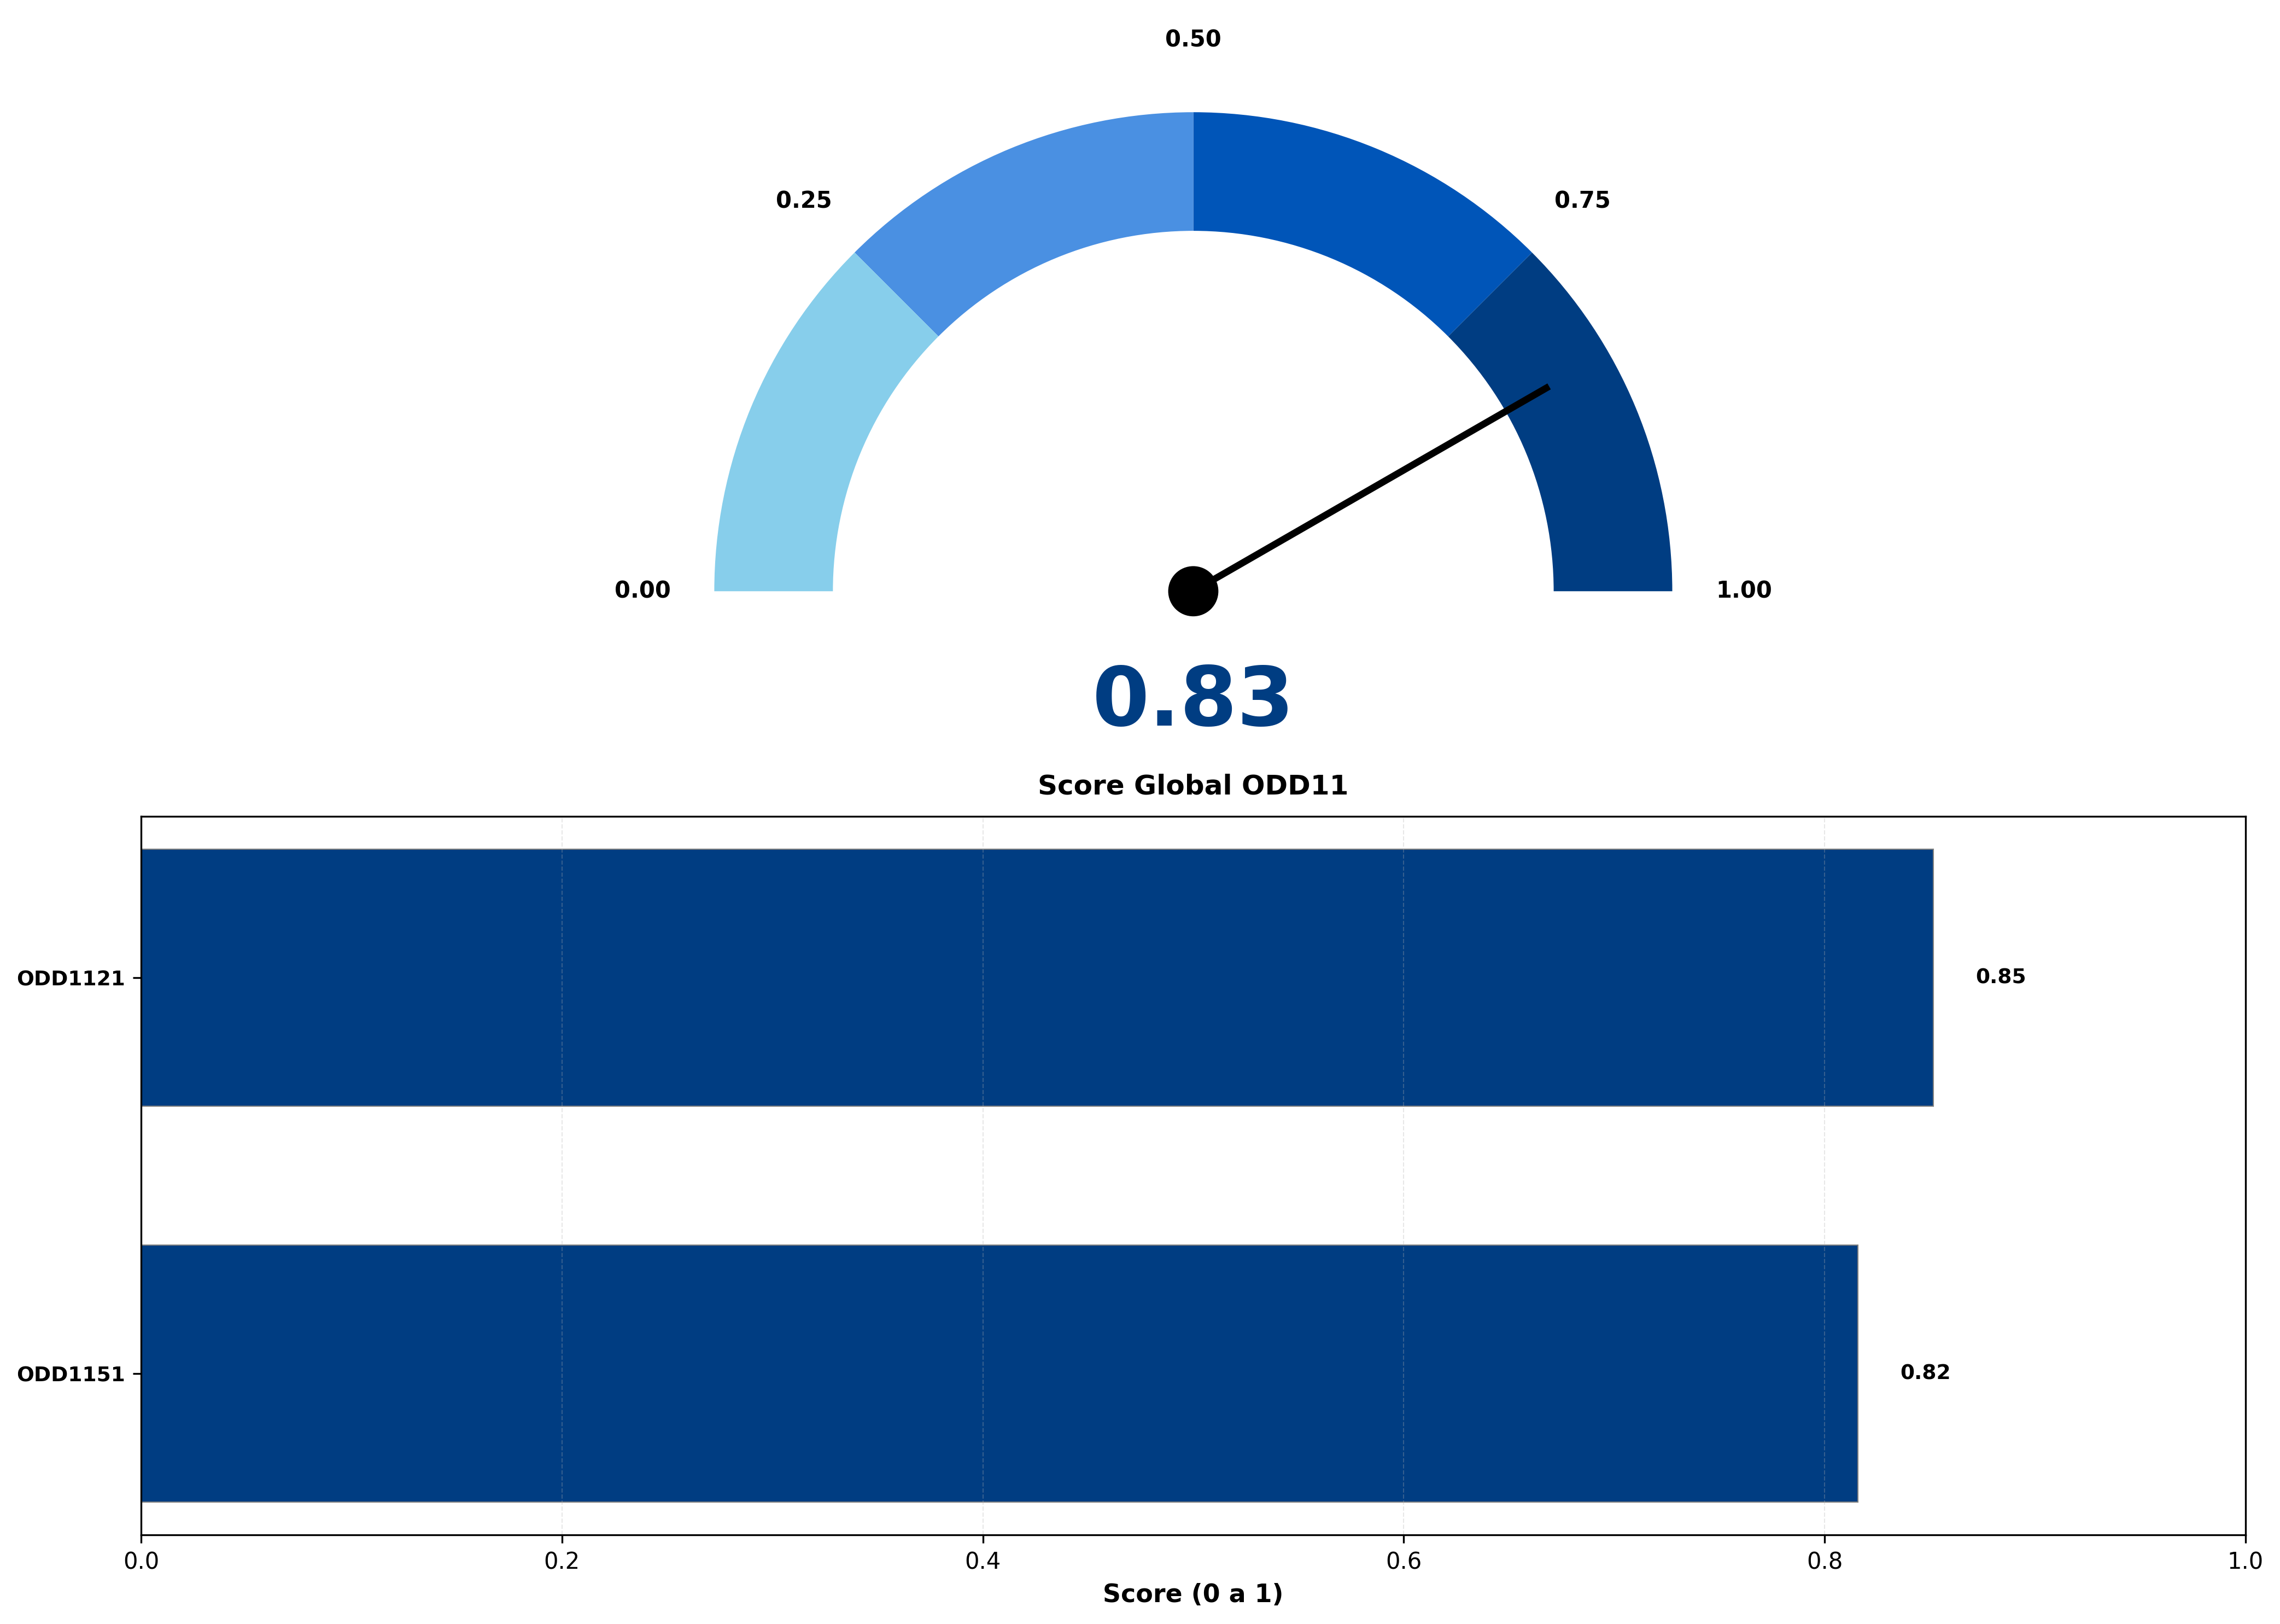
\includegraphics[width=0.95\textwidth]{Pictures/graphs/ODD11_scores.png}
	\caption{Performance par indicateur - ODD11}
\end{figure}

\begin{table}[H]
	\centering
	\begin{tabularx}{\textwidth}{l l c c c}
		\rowcolor[HTML]{003D82}
		\color{white}\textbf{Code} & \color{white}\textbf{Indicateur} & \color{white}\textbf{Valeur} & \color{white}\textbf{Cible} & \color{white}\textbf{Score} \\
		\rowcolor[HTML]{F5F8FC}
		ODD1151 & Victimes de catastrophes & 0.18 & 0.00 & 0.82 \\
		\rowcolor[HTML]{E8F0FF}
		ODD1121 & Accès aisé aux services de transports & 0.86 & 1.00 & 0.85 \\
	\end{tabularx}
\end{table}

L'analyse du ODD11 révèle un score global de 0.8337, basé sur 2 indicateur(s). Les performances varient de 0.82 à 0.85, montrant une certaine disparité dans la mise en oeuvre des cibles. Les indicateurs critiques (score < 0,30) nécessitent une attention particulière.


%%%%%%%%%%%%%%%%%%%%% ODD12 %%%%%%%%%%%%%%%%%%%%%%%%%%%

\newpage
\begin{simplebox2}
	
	\begin{minipage}{0.15\textwidth}
		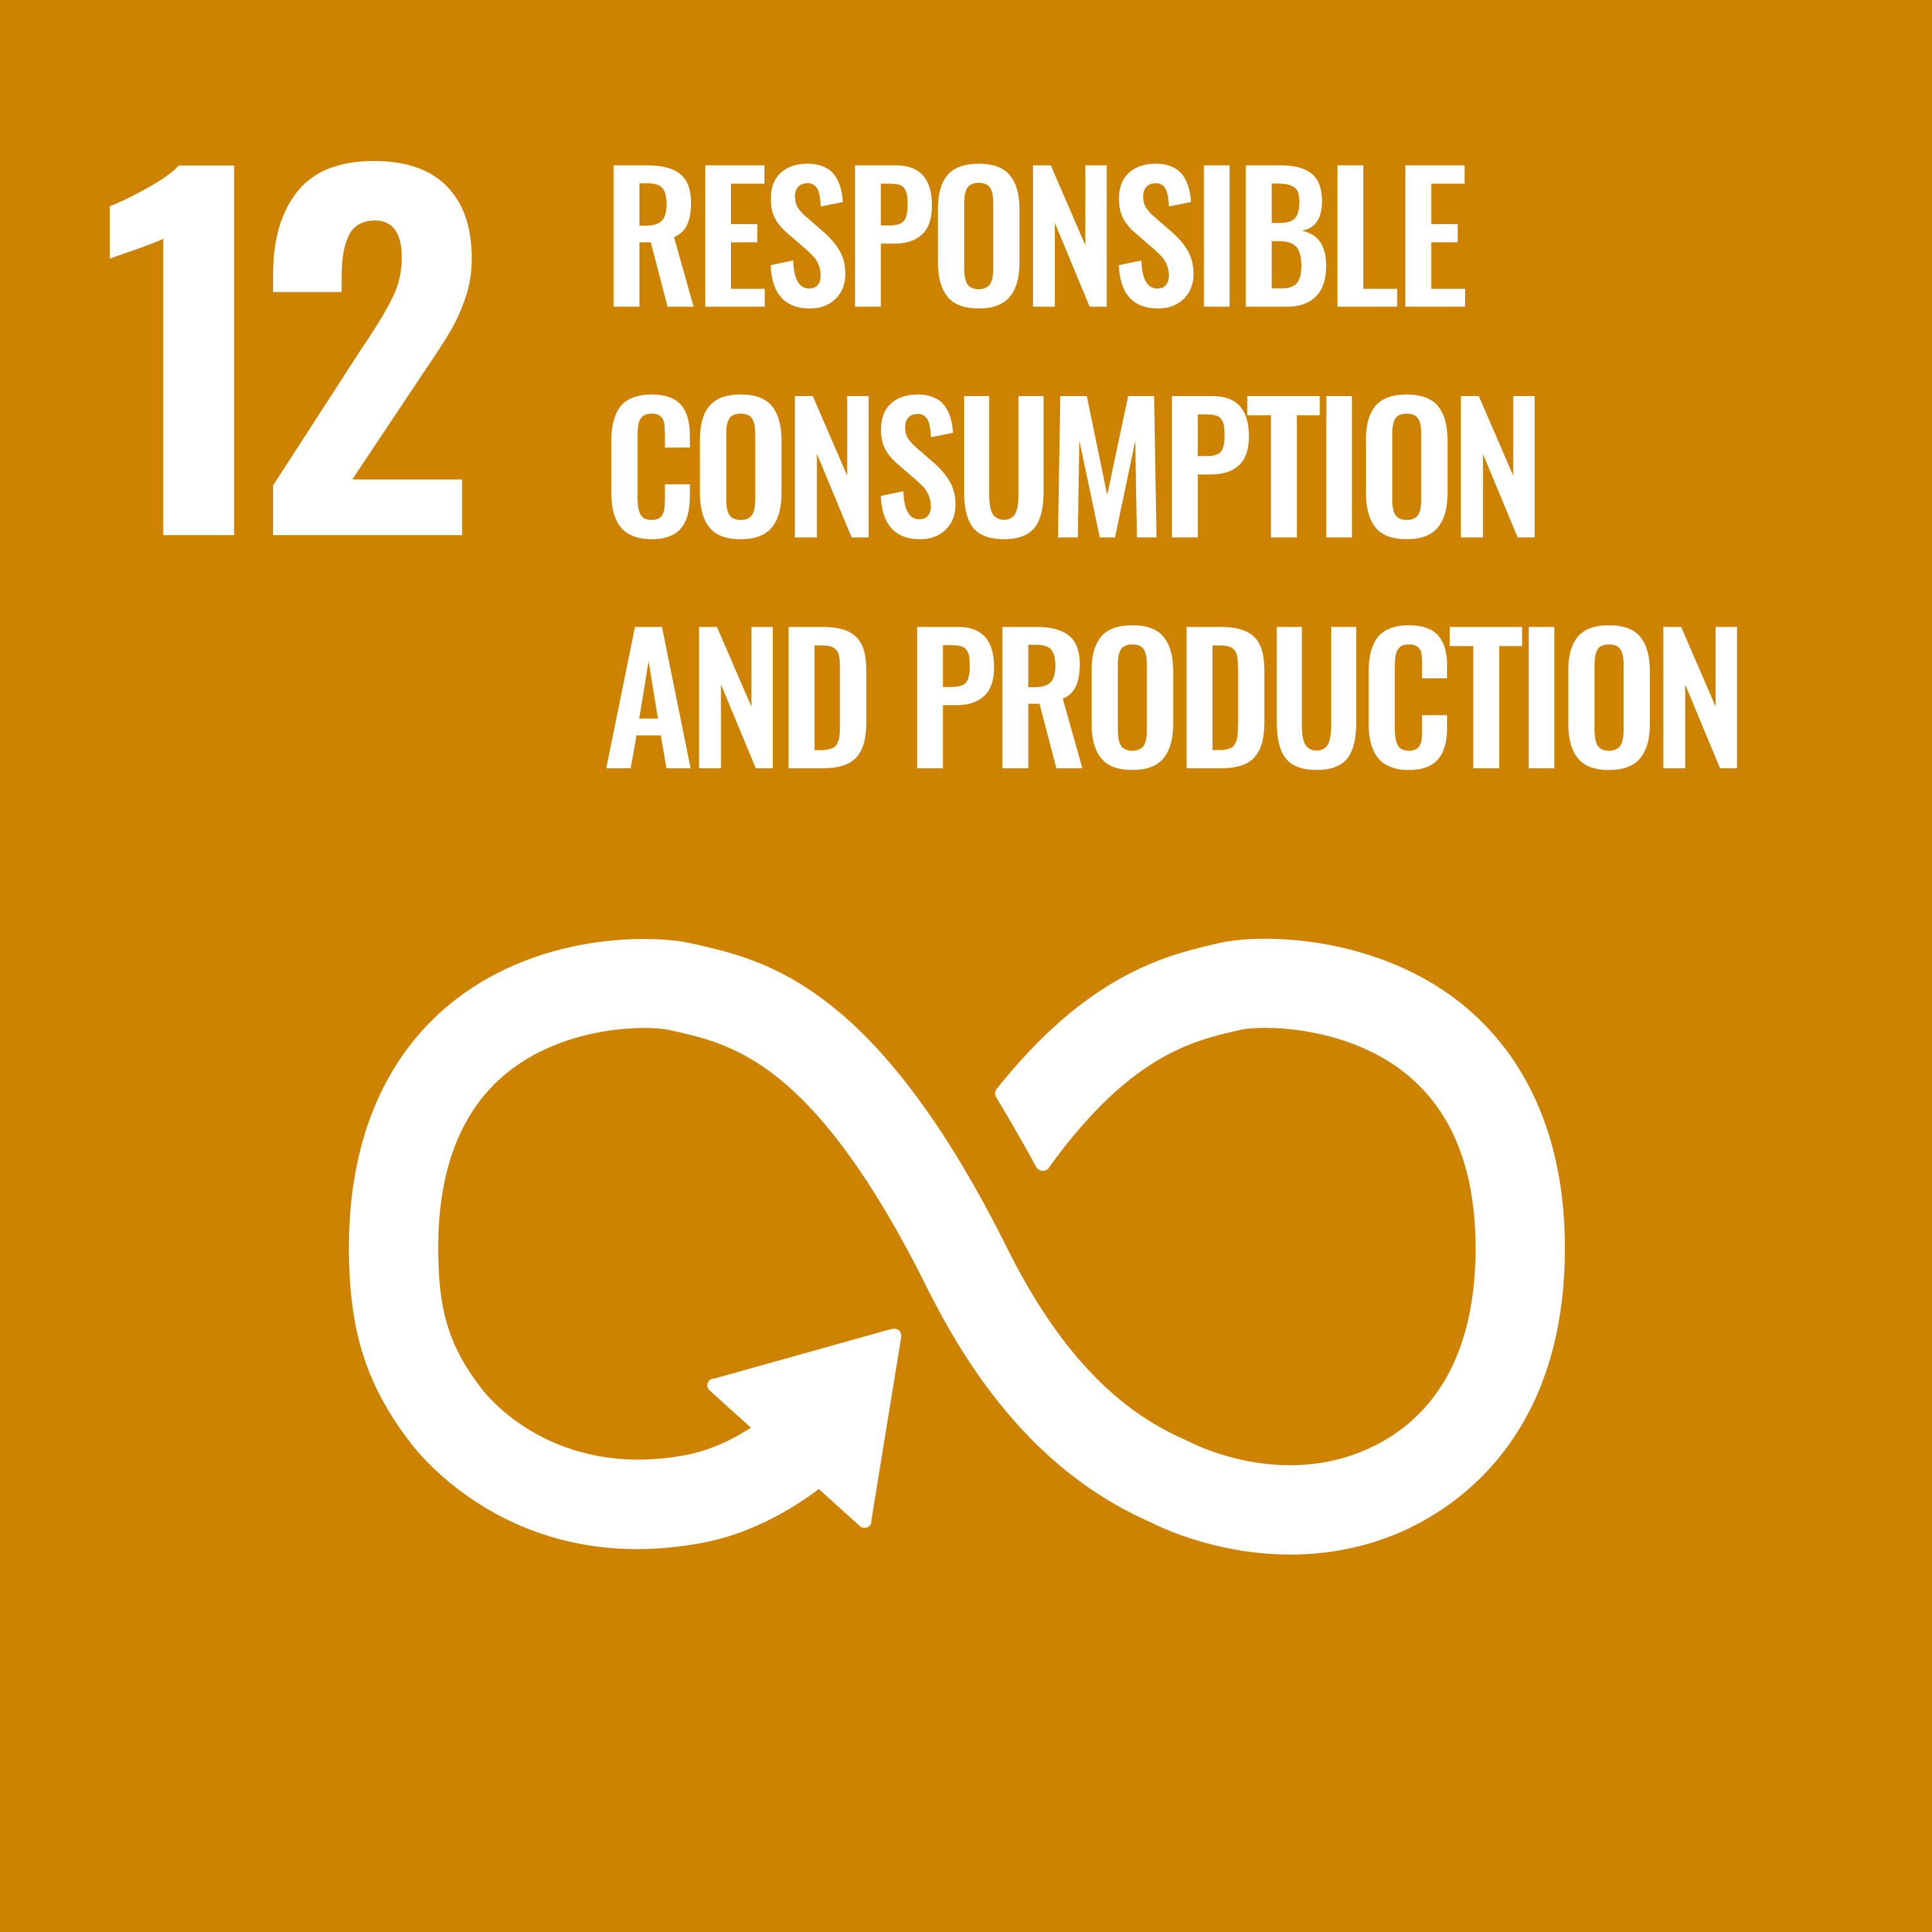
\includegraphics[width=\linewidth]{Pictures/ODD/ODD12.jpg}
	\end{minipage}
	\hfill
	\begin{minipage}{0.8\textwidth}
		{\bfseries\Large ODD 12 : }\\[2pt]
		\textit{Établir des modes de consommation et de production durables.}
	\end{minipage}
\end{simplebox2}



\section{Cible 12.2 : Utilisation durable des ressources naturelles}

La cible 12.2 vise à parvenir à une gestion durable et à une utilisation efficace des ressources naturelles.

\begin{figure}[H]
	\centering
	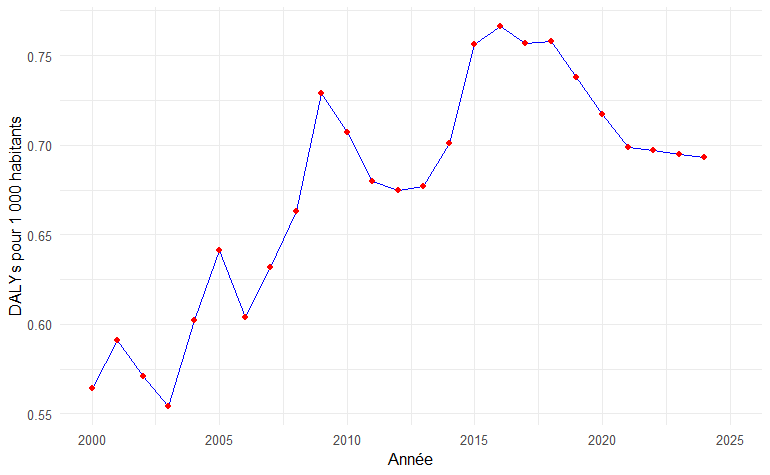
\includegraphics[width=0.75\textwidth]{Pictures/graphs/sdg12_pollprod.png}
	\caption{Évolution de la pollution atmosphérique liée à la production nationale}
	\label{fig:od12_pollprod}
\end{figure}

L’évolution de la pollution atmosphérique liée à la production nationale montre des valeurs relativement stables sur la période étudiée. Cela traduit une production industrielle constante, avec un impact environnemental qui reste modéré mais qui nécessite un suivi continu pour éviter toute détérioration, notamment en période de croissance économique.

\section{Cible 12.4 : Réduction des impacts environnementaux des produits chimiques et polluants}

La cible 12.4 vise à réduire substantiellement la libération de produits chimiques et de polluants dans l’air, l’eau et le sol, afin de minimiser les impacts négatifs sur la santé humaine et l’environnement.

\begin{figure}[H]
	\centering
	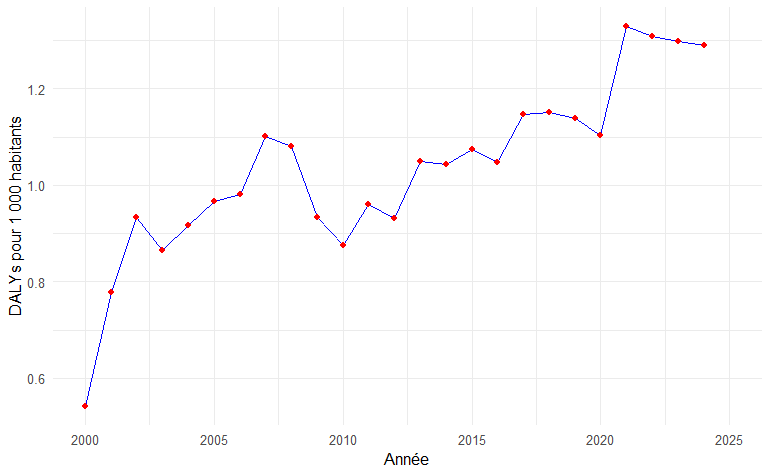
\includegraphics[width=0.75\textwidth]{Pictures/graphs/sdg12_pollimp.png}
	\caption{Évolution de la pollution atmosphérique associée aux produits importés}
	\label{fig:od12_pollimp}
\end{figure}

La pollution générée par les produits importés présente une tendance à la hausse et une certaine volatilité. Cela indique que, bien que la production locale soit relativement maîtrisée, les importations de biens contribuent de manière croissante à l’exposition de la population à des polluants, soulignant la nécessité de politiques visant à contrôler et réduire l’impact des importations sur l’environnement.


\section*{Synthèse}

Dans l’ensemble, le Sénégal présente une stabilité relative dans ses impacts environnementaux domestiques, mais les importations contribuent de façon croissante à la pollution et aux émissions d’azote. Pour atteindre les cibles de consommation et de production responsables, il est essentiel de combiner la réduction des émissions locales avec un contrôle plus strict des flux importés et la promotion de pratiques durables dans toute la chaîne de production et de consommation.

\section*{Synthèse de la performance - ODD12}

\begin{figure}[H]
	\centering
	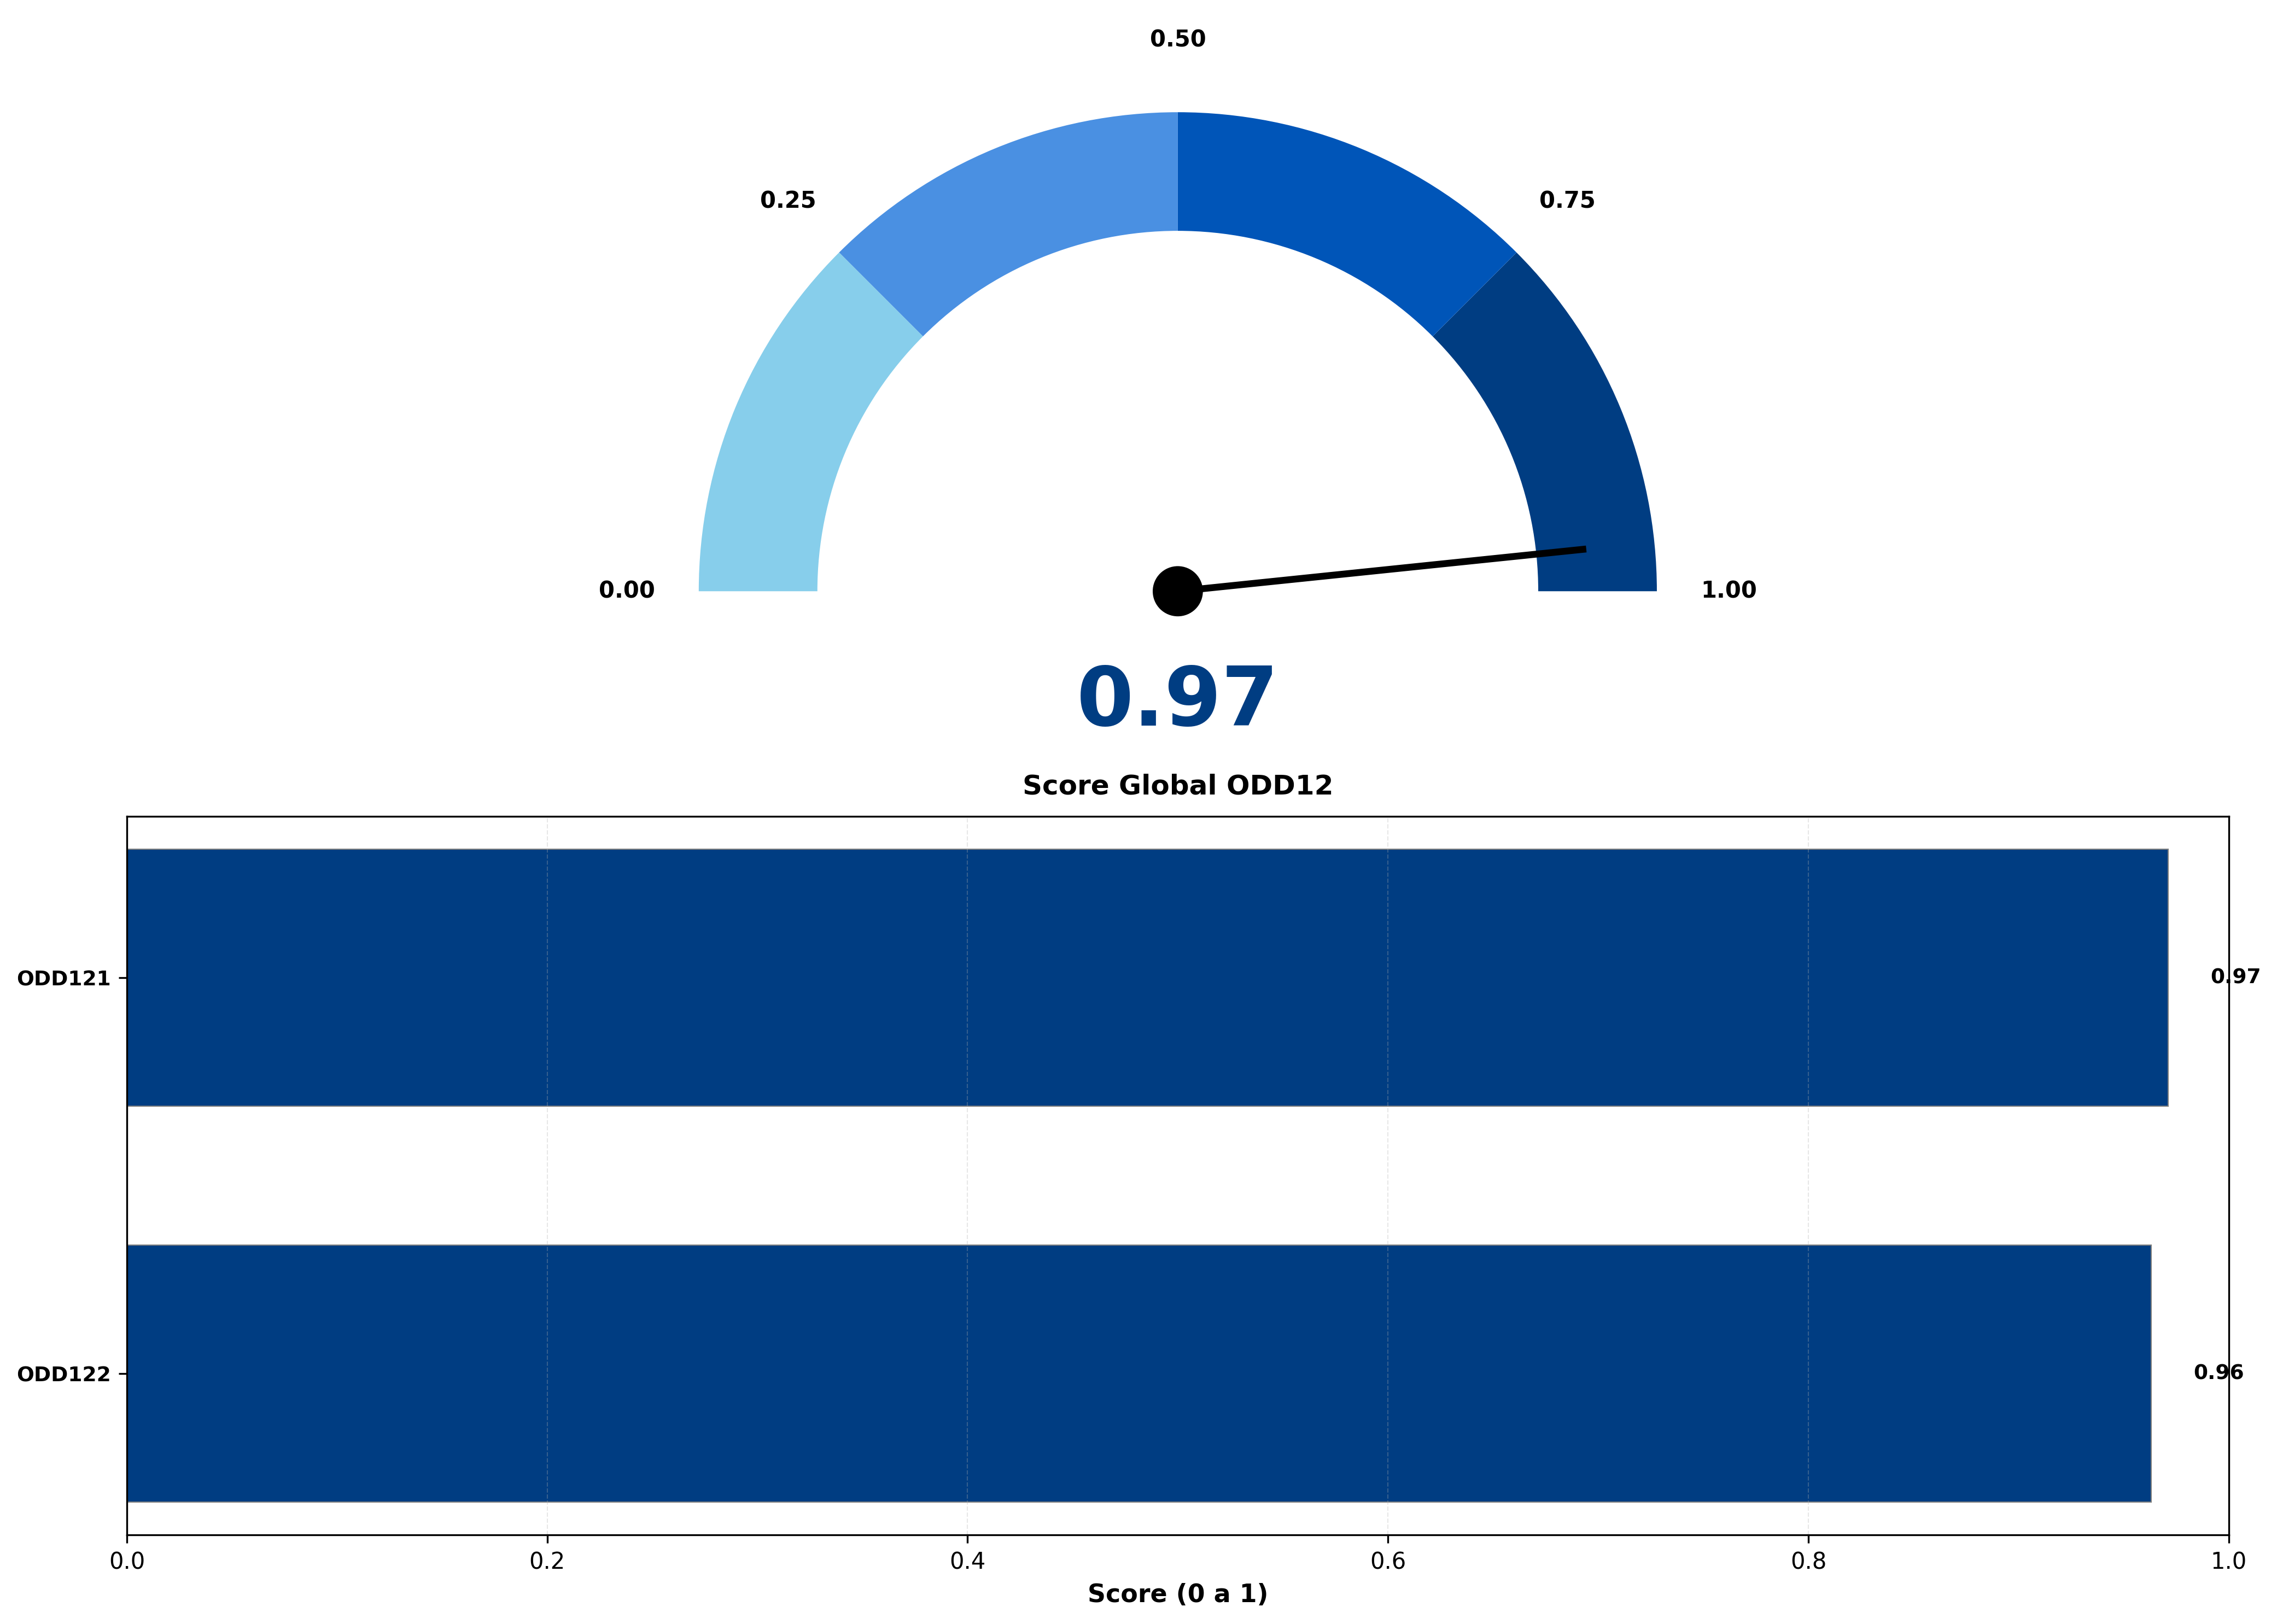
\includegraphics[width=0.95\textwidth]{Pictures/graphs/ODD12_scores.png}
	\caption{Performance par indicateur - ODD12}
\end{figure}

\begin{table}[H]
	\centering
	\begin{tabularx}{\textwidth}{l l c c c}
		\rowcolor[HTML]{003D82}
		\color{white}\textbf{Code} & \color{white}\textbf{Indicateur} & \color{white}\textbf{Valeur} & \color{white}\textbf{Cible} & \color{white}\textbf{Score} \\
		\rowcolor[HTML]{F5F8FC}
		ODD121& Pollution de l'air associée à la production & 0.69 & 0.00 & 0.97 \\
		ODD122& Pollution de l'air associé à l'importation & 1.29 & 0.00 & 0.96 \\
	\end{tabularx}
\end{table}

L'analyse du ODD12 révèle un score global de 0.9712, basé sur 1 indicateur(s). Les performances varient de 0.97 à 0.97, montrant une certaine disparité dans la mise en oeuvre des cibles. Les indicateurs critiques (score < 0,30) nécessitent une attention particulière.


%%%%%%%%%%%%%%%%%%%%% ODD13 %%%%%%%%%%%%%%%%%%%%%%%%%%%

\newpage
\begin{simplebox2}
	
	\begin{minipage}{0.15\textwidth}
		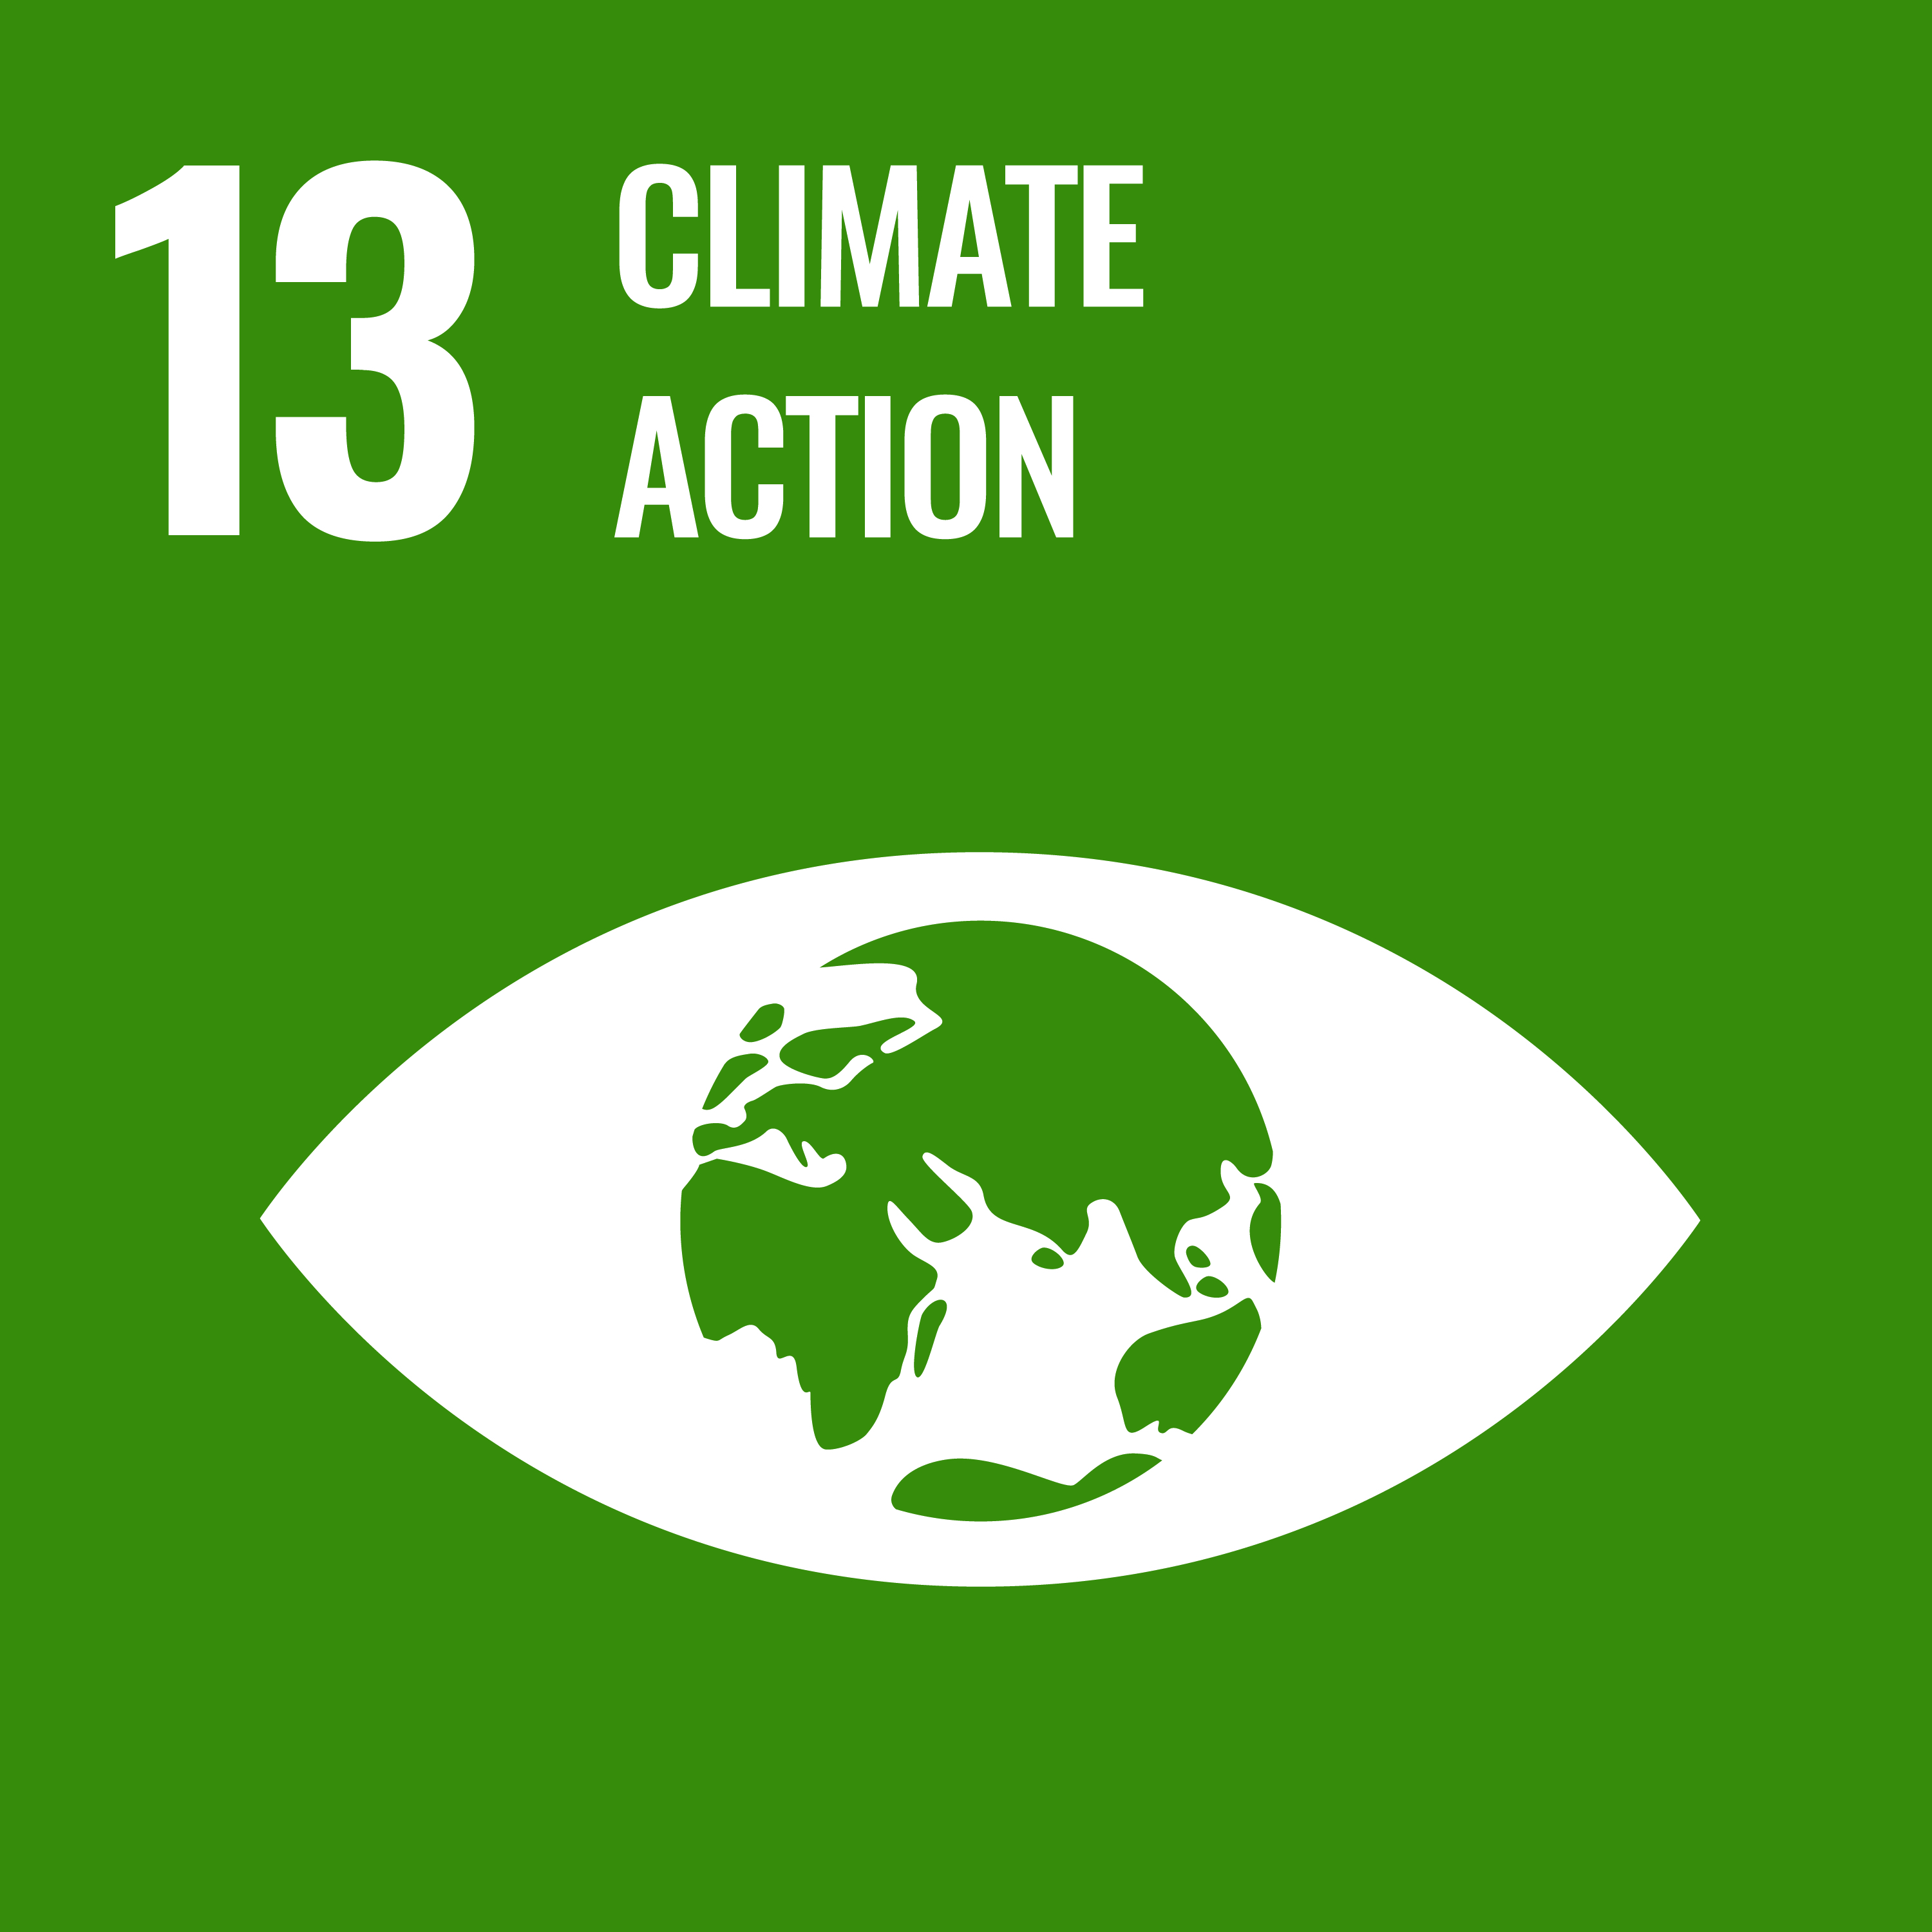
\includegraphics[width=\linewidth]{Pictures/ODD/ODD13.jpg}
	\end{minipage}
	\hfill
	\begin{minipage}{0.8\textwidth}
		{\bfseries\Large ODD 13 : }\\[2pt]
		\textit{Prendre d’urgence des mesures pour lutter contre les changements climatiques et leurs répercussions.}
	\end{minipage}
\end{simplebox2}



\section{Cible 13.2 : Intégration des mesures de lutte contre le changement climatique}

La cible 13.2 vise à intégrer des mesures de lutte contre le changement climatique dans les politiques, stratégies et planifications nationales.

\begin{figure}[H]
	\centering
	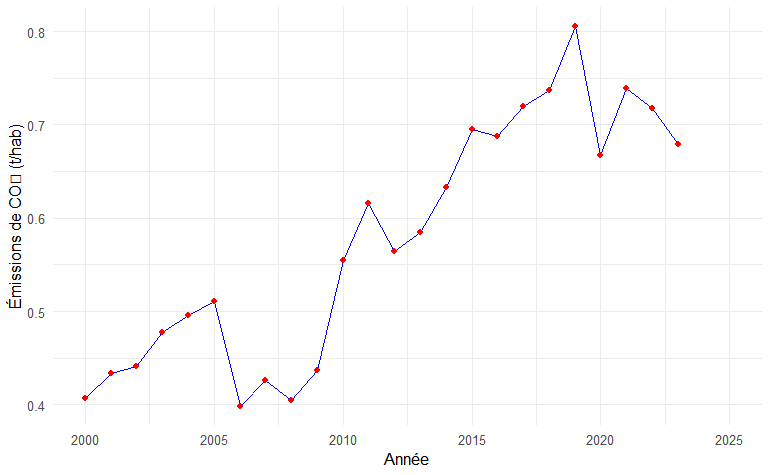
\includegraphics[width=0.75\textwidth]{Pictures/graphs/sdg13_co2gcp.png}
	\caption{Évolution des émissions de CO$_{2}$ provenant de la combustion des énergies fossiles et de la production de ciment par habitant}
	\label{fig:od13_co2gcp}
\end{figure}

Les émissions de CO$_{2}$ par habitant provenant des activités locales montrent une tendance à la hausse sur la période étudiée, passant d’environ 0,41 à 0,74 tonnes par habitant. Cette augmentation indique que la croissance économique et l’urbanisation s’accompagnent d’une demande énergétique croissante, soulignant l’importance d’intégrer davantage de solutions bas-carbone et de promouvoir l’efficacité énergétique pour atteindre les objectifs climatiques.

\section{Cible 13.3 : Sensibilisation et renforcement des capacités}

La cible 13.3 vise à renforcer les connaissances et la capacité d’adaptation des populations face au changement climatique, notamment en prenant en compte l’impact des importations.

\begin{figure}[H]
	\centering
	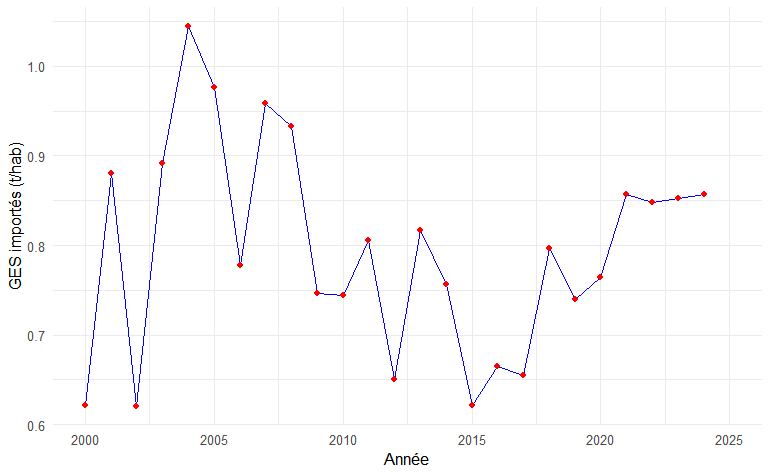
\includegraphics[width=0.75\textwidth]{Pictures/graphs/sdg13_ghgimport.png}
	\caption{Évolution des émissions de gaz à effet de serre liées aux importations par habitant}
	\label{fig:od13_ghgimport}
\end{figure}

Les émissions de gaz à effet de serre associées aux importations présentent une tendance générale à la hausse et une certaine volatilité, atteignant jusqu’à 1,04 tonnes par habitant. Cela reflète l’impact indirect de la consommation de biens importés sur l’empreinte carbone nationale et met en évidence la nécessité de politiques favorisant des importations plus durables et une consommation responsable pour réduire la vulnérabilité climatique du pays.



\subsection*{Synthèse}

Globalement, le Sénégal connaît une augmentation progressive des émissions directes et indirectes de gaz à effet de serre. Ces tendances montrent que des efforts supplémentaires sont nécessaires, tant au niveau national que dans la gestion des importations, pour atteindre les objectifs climatiques et limiter les impacts négatifs du changement climatique sur la population et l’environnement.

\section*{Synthèse de la performance - ODD13}

\begin{figure}[H]
	\centering
	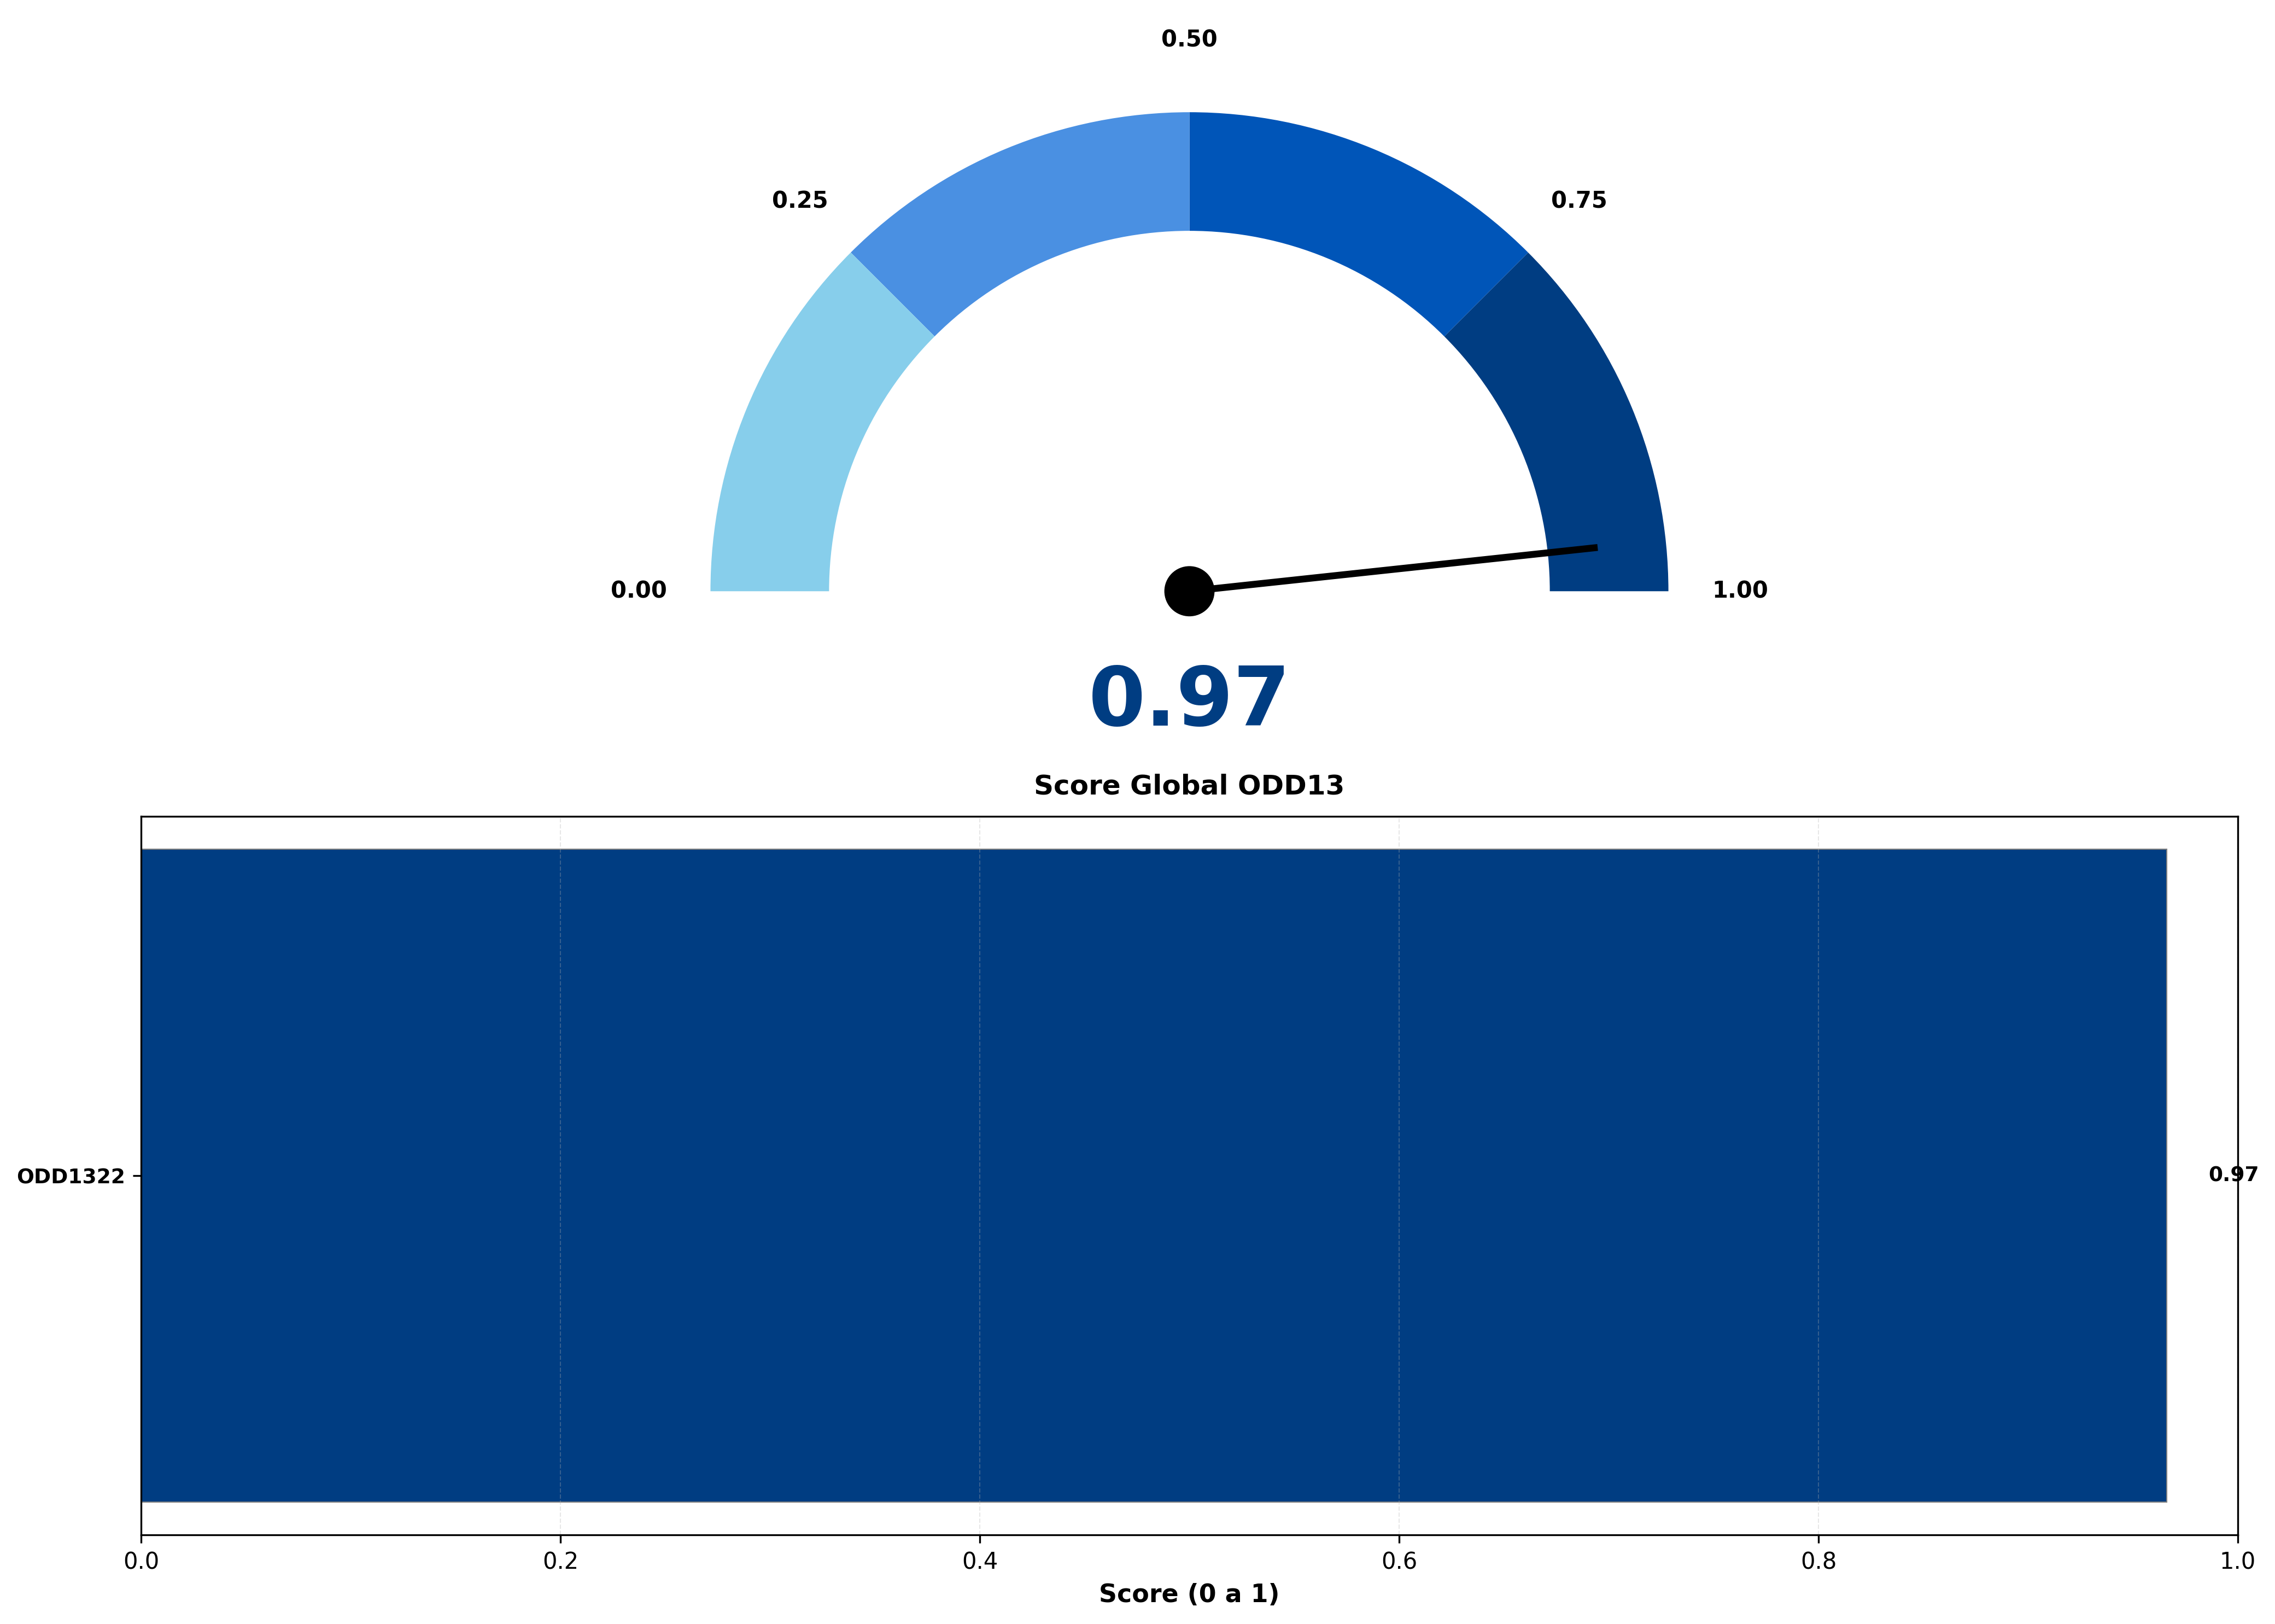
\includegraphics[width=0.95\textwidth]{Pictures/graphs/ODD13_scores.png}
	\caption{Performance par indicateur - ODD13}
\end{figure}

\begin{table}[H]
	\centering
	\begin{tabularx}{0.85\textwidth}{l l c c c}
		\rowcolor[HTML]{003D82}
		\color{white}\textbf{Code} & \color{white}\textbf{Indicateur} & \color{white}\textbf{Valeur} & \color{white}\textbf{Cible} & \color{white}\textbf{Score} \\
		\rowcolor[HTML]{F5F8FC}
		ODD1322 & Emission de gaz à effet de serre & 0.68 & 0.00 & 0.97 \\
	\end{tabularx}
\end{table}

L'analyse du ODD13 révèle un score global de 0.9660, basé sur 1 indicateur(s). Les performances varient de 0.97 à 0.97, montrant une certaine disparité dans la mise en oeuvre des cibles. Les indicateurs critiques (score < 0,30) nécessitent une attention particulière.

%%%%%%%%%%%%%%%%%%%%% ODD14 %%%%%%%%%%%%%%%%%%%%%%%%%%%

\newpage
\begin{simplebox2}
	
	\begin{minipage}{0.15\textwidth}
		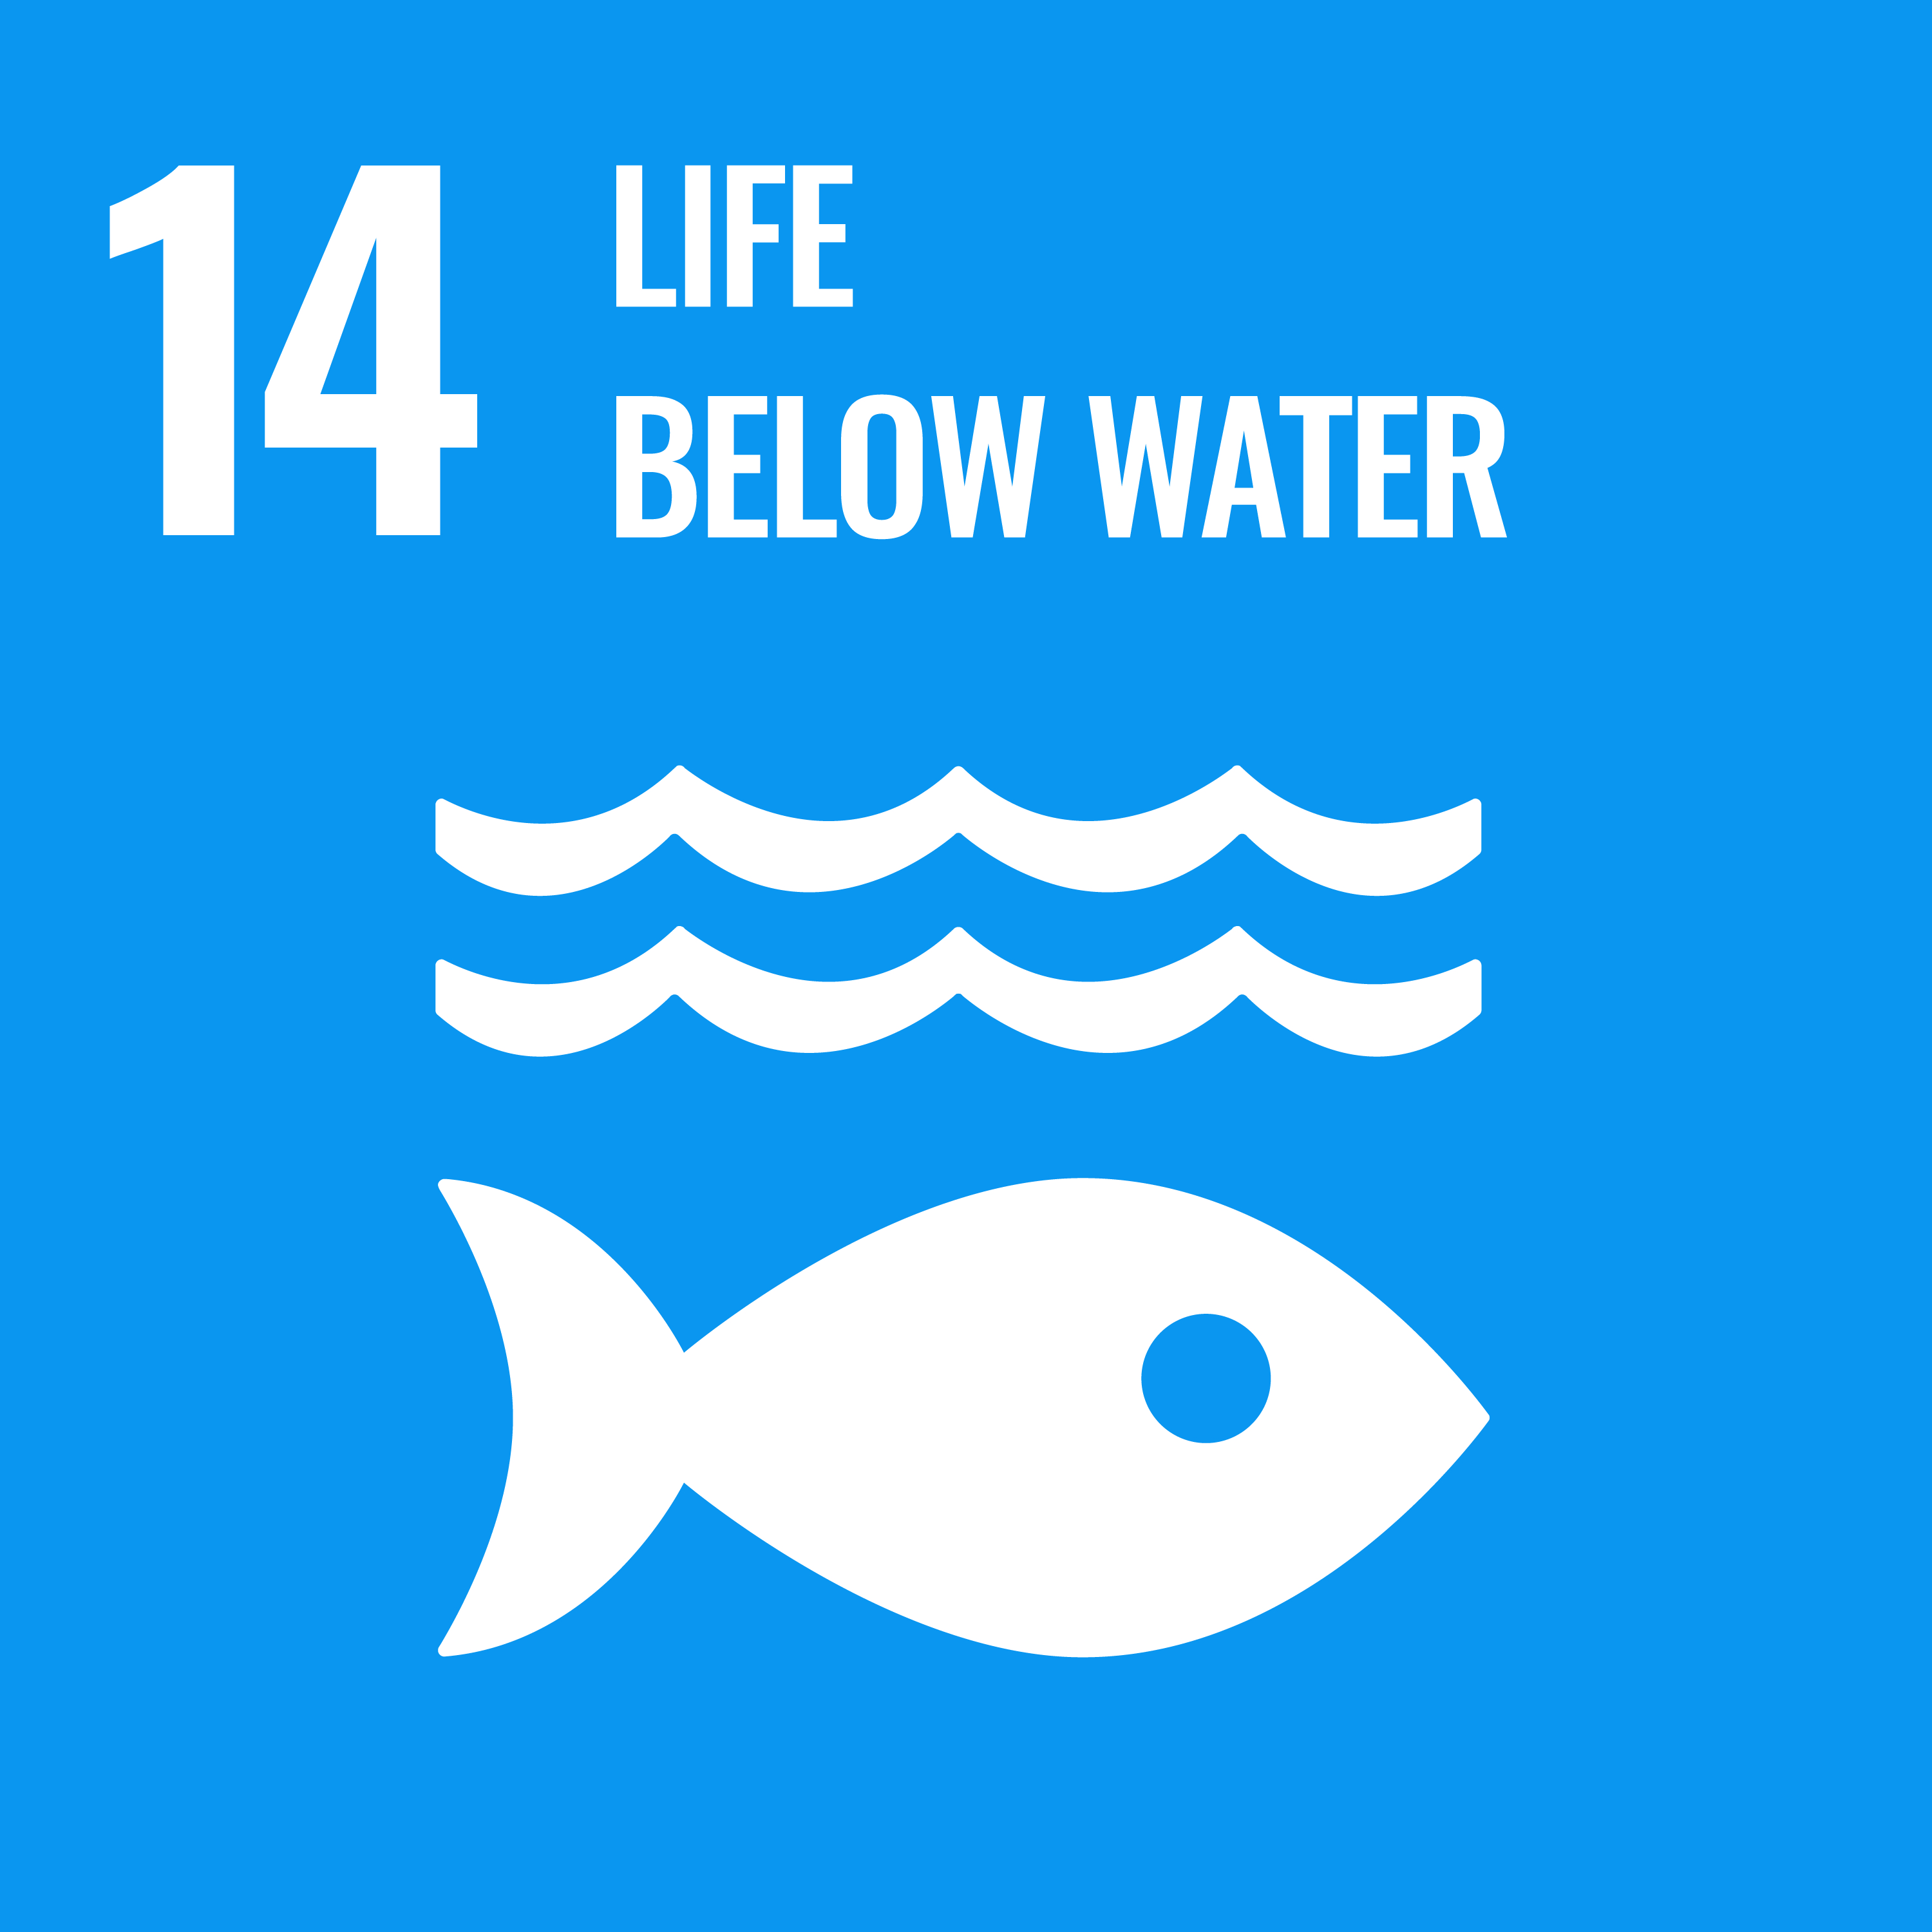
\includegraphics[width=\linewidth]{Pictures/ODD/ODD14.jpg}
	\end{minipage}
	\hfill
	\begin{minipage}{0.8\textwidth}
		{\bfseries\Large ODD 14 : }\\[2pt]
		\textit{Conserver et exploiter de manière durable les océans, les mers et les ressources marines aux fins du développement durable.}
	\end{minipage}
\end{simplebox2}

\section{Vie acquatique}

\subsection{Cible 14.2 : Protection des écosystèmes marins}

La cible 14.2 vise à protéger les écosystèmes marins et côtiers, en limitant la dégradation et en restaurer les habitats essentiels pour la biodiversité.

\begin{figure}[H]
	\centering
	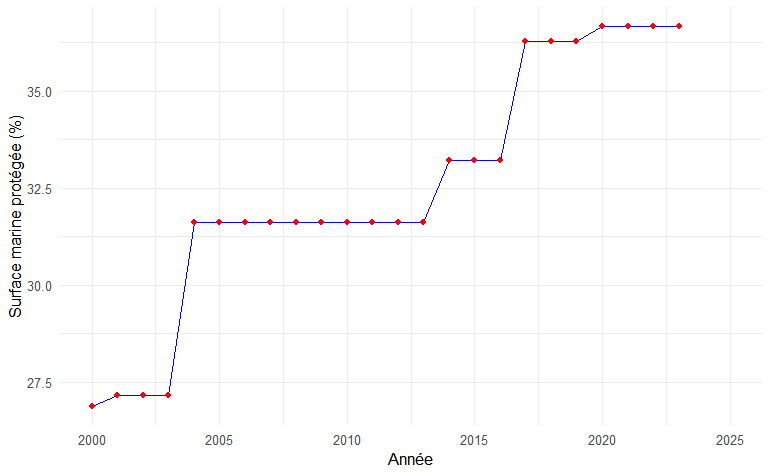
\includegraphics[width=0.75\textwidth]{Pictures/graphs/sdg14_cpma.png}
	\caption{Évolution de la surface protégée dans les sites marins importants pour la biodiversité}
	\label{fig:od14_cpma}
\end{figure}

La part de la surface marine protégée a progressé au fil du temps, passant d’environ 27\% à 36\%. Cette évolution traduit les efforts du Sénégal pour conserver les zones marines et protéger la biodiversité, bien que l’objectif idéal de 100\% reste loin d’être atteint.

\subsection{Cible 14.4 : Gestion durable de la pêche}

La cible 14.4 vise à réguler la pêche afin d’assurer des stocks de poissons durables et à mettre fin à la surpêche.

\begin{figure}[H]
	\centering
	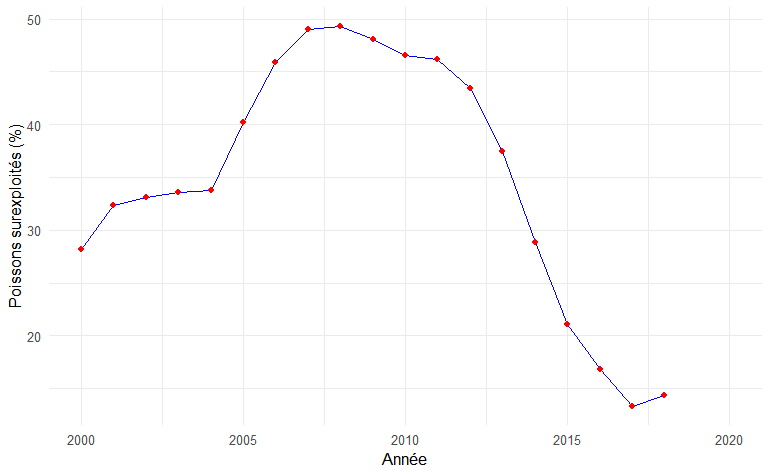
\includegraphics[width=0.75\textwidth]{Pictures/graphs/sdg14_fishstocks.png}
	\caption{Évolution du pourcentage de poissons provenant de stocks surexploités ou effondrés}
	\label{fig:od14_fishstocks}
\end{figure}

Le pourcentage de poissons issus de stocks surexploités ou effondrés montre une tendance générale à la baisse, passant d’environ 32\% à 14\%. Cela indique une amélioration de la gestion des ressources halieutiques, mais la surpêche reste un enjeu à surveiller pour atteindre la durabilité complète des stocks.

\begin{figure}[H]
	\centering
	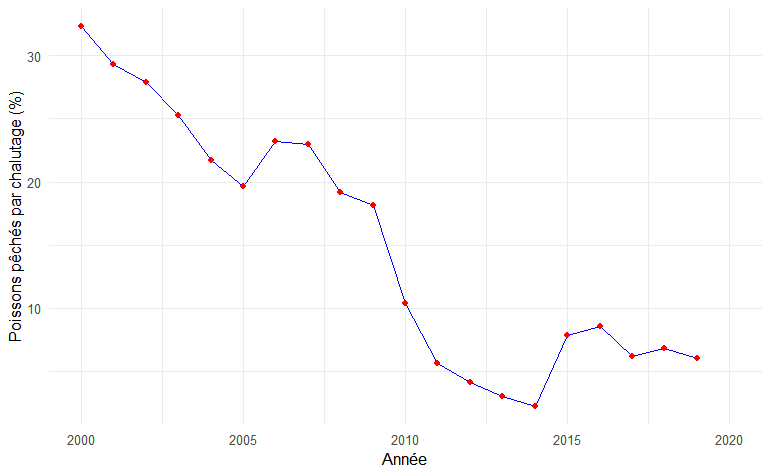
\includegraphics[width=0.75\textwidth]{Pictures/graphs/sdg14_trawl.png}
	\caption{Évolution du pourcentage de poissons pêchés par chalutage ou dragage}
	\label{fig:od14_trawl}
\end{figure}

La proportion de poissons capturés par des techniques destructrices comme le chalutage ou le dragage tend à diminuer, ce qui est favorable à la protection des fonds marins et à la biodiversité. Cependant, certaines années montrent des fluctuations, soulignant la nécessité de régulations strictes et d’une surveillance continue.

\subsection*{Synthèse}

Dans l’ensemble, les efforts du Sénégal pour protéger les écosystèmes marins et gérer durablement la pêche montrent des résultats positifs : augmentation des surfaces protégées et diminution de la surexploitation des stocks. Cependant, des marges importantes existent encore pour atteindre les objectifs internationaux fixés par l’ODD 14.


\section*{Synthèse de la performance - ODD14}

\begin{figure}[H]
	\centering
	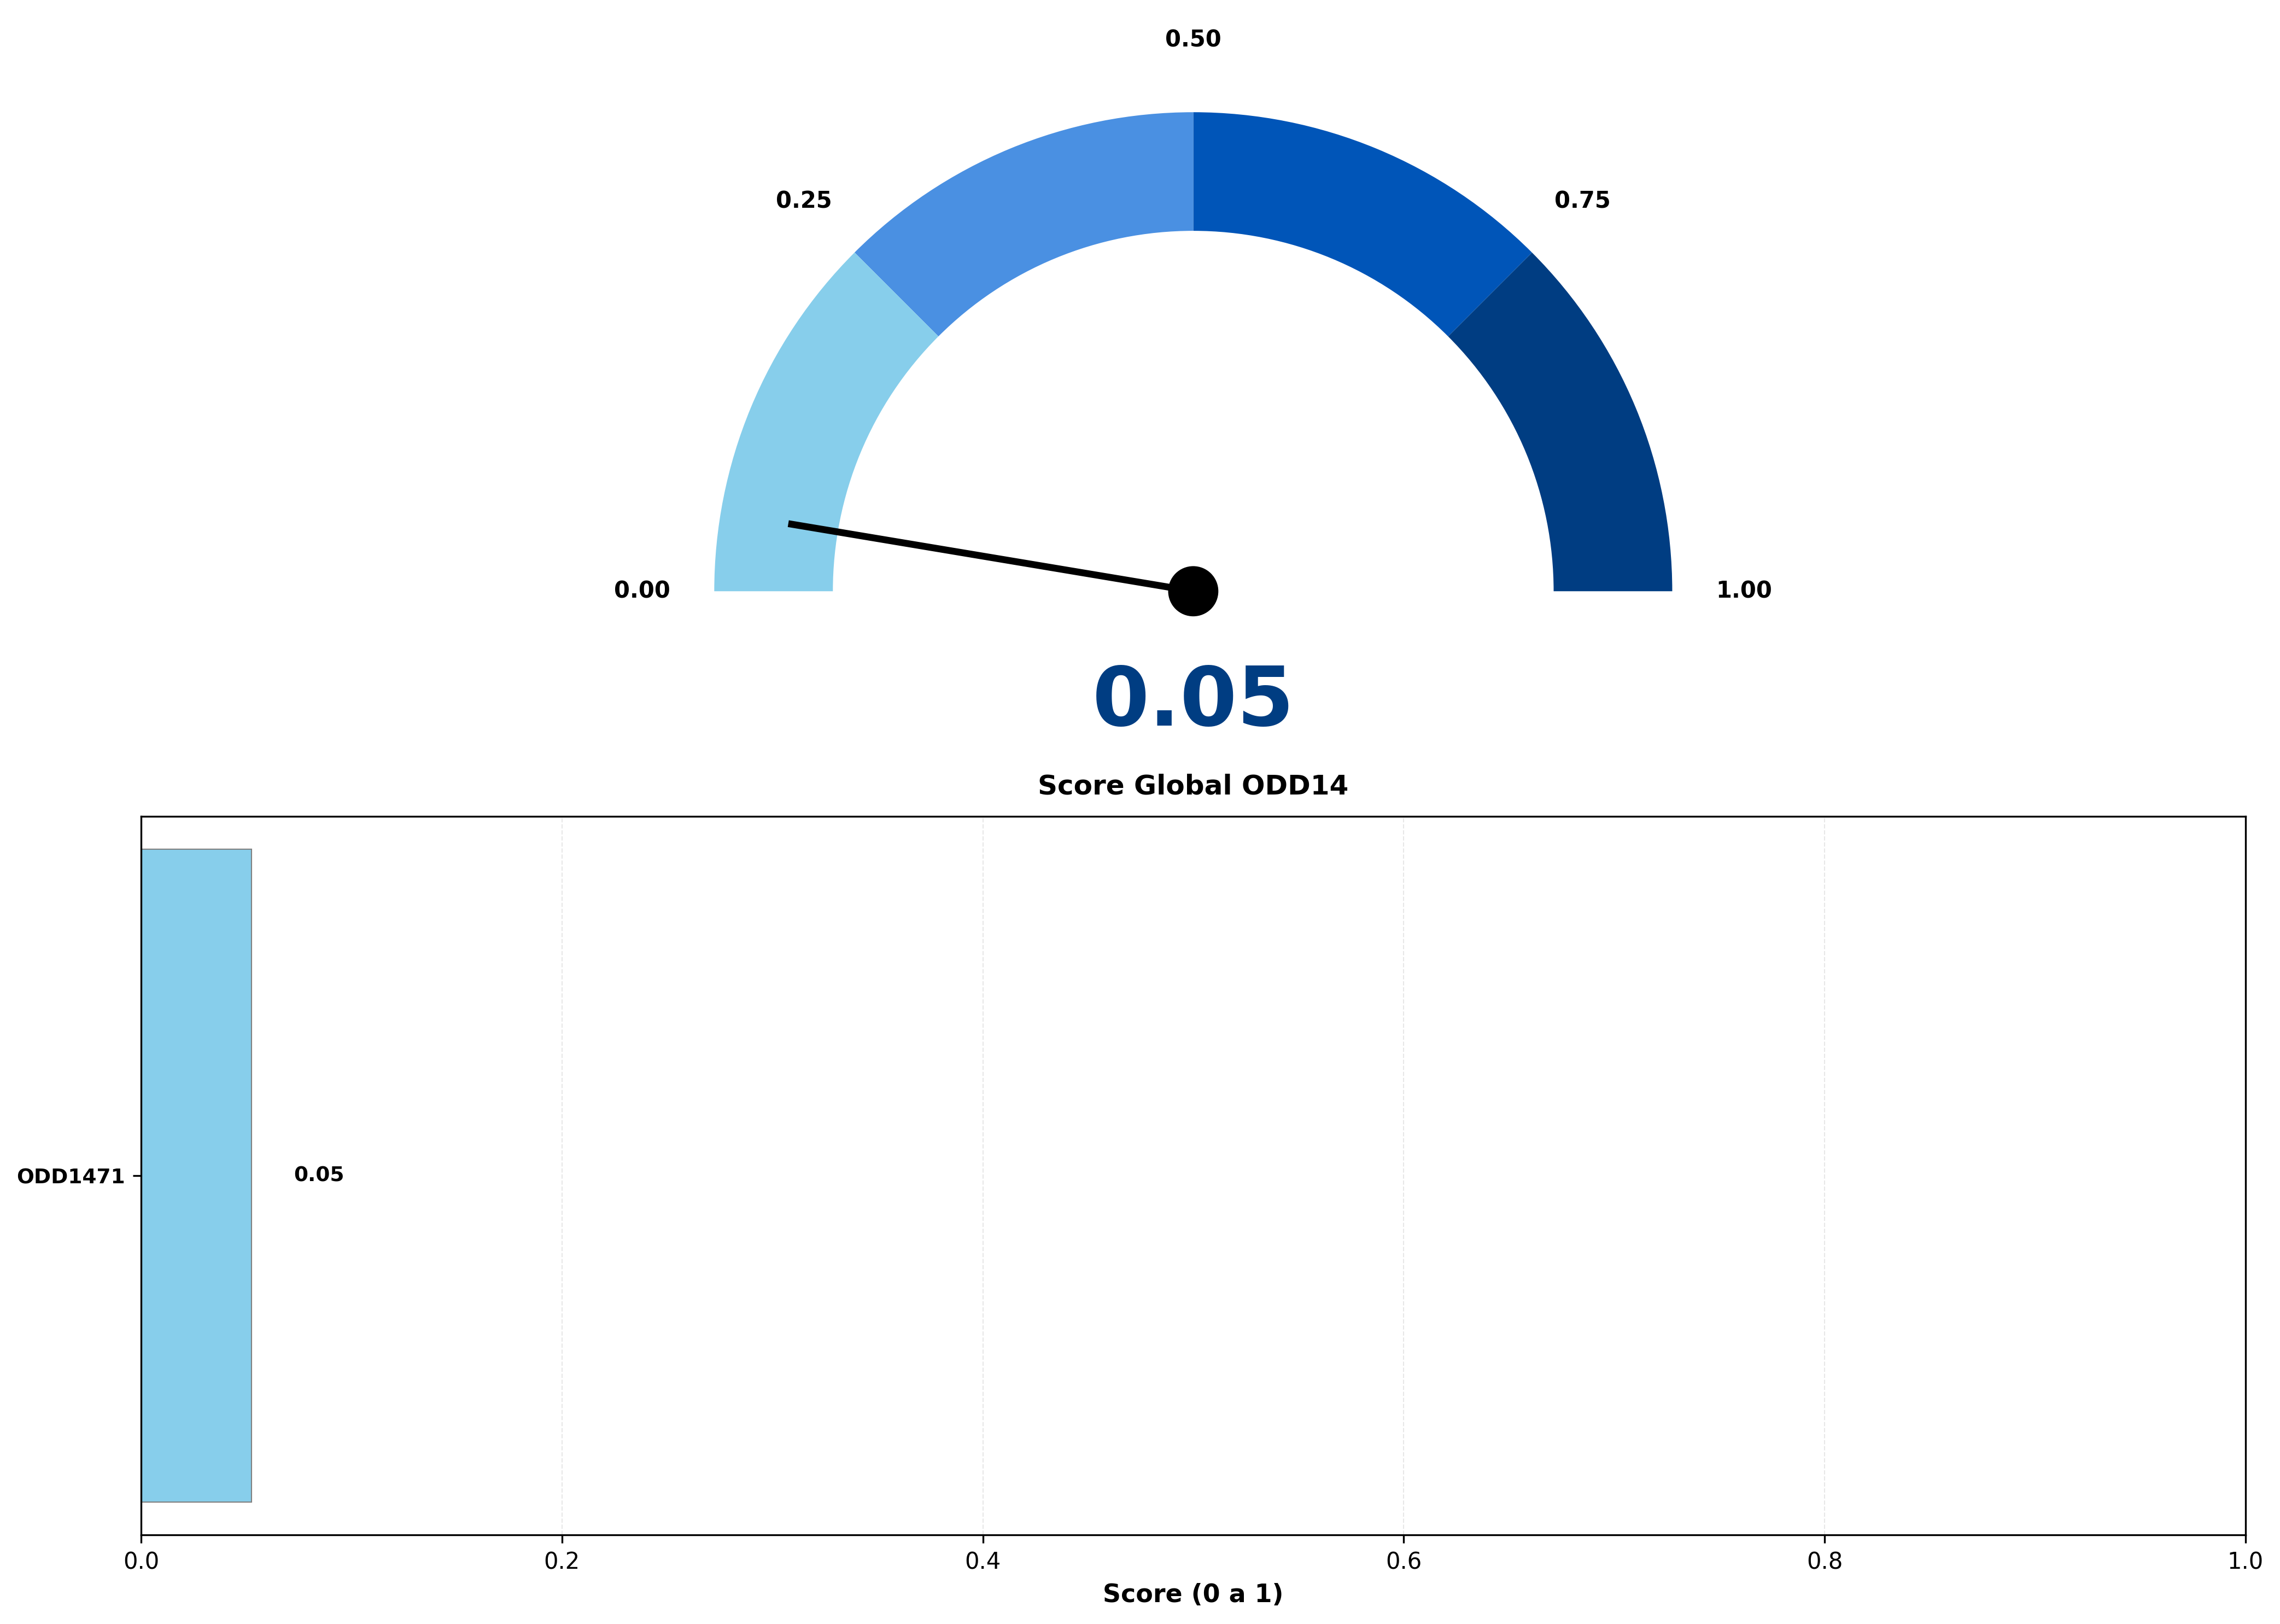
\includegraphics[width=0.95\textwidth]{Pictures/graphs/ODD14_scores.png}
	\caption{Performance par indicateur - ODD14}
\end{figure}

\begin{table}[H]
	\centering
	\begin{tabularx}{0.85\textwidth}{l l c c c}
		\rowcolor[HTML]{003D82}
		\color{white}\textbf{Code} & \color{white}\textbf{Indicateur} & \color{white}\textbf{Valeur} & \color{white}\textbf{Cible} & \color{white}\textbf{Score} \\
		\rowcolor[HTML]{F5F8FC}
		ODD1471 & Part de la VA de la pêche et de l'Aquaculture & 0.01 & 0.10 & 0.05 \\
	\end{tabularx}
\end{table}

L'analyse du ODD14 révèle un score global de 0.0526, basé sur 1 indicateur(s). Les performances varient de 0.05 à 0.05, montrant une certaine disparité dans la mise en oeuvre des cibles. Les indicateurs critiques (score < 0,30) nécessitent une attention particulière.


%%%%%%%%%%%%%%%%%%%%% ODD15 %%%%%%%%%%%%%%%%%%%%%%%%%%%

\newpage
\begin{simplebox2}
	
	\begin{minipage}{0.15\textwidth}
		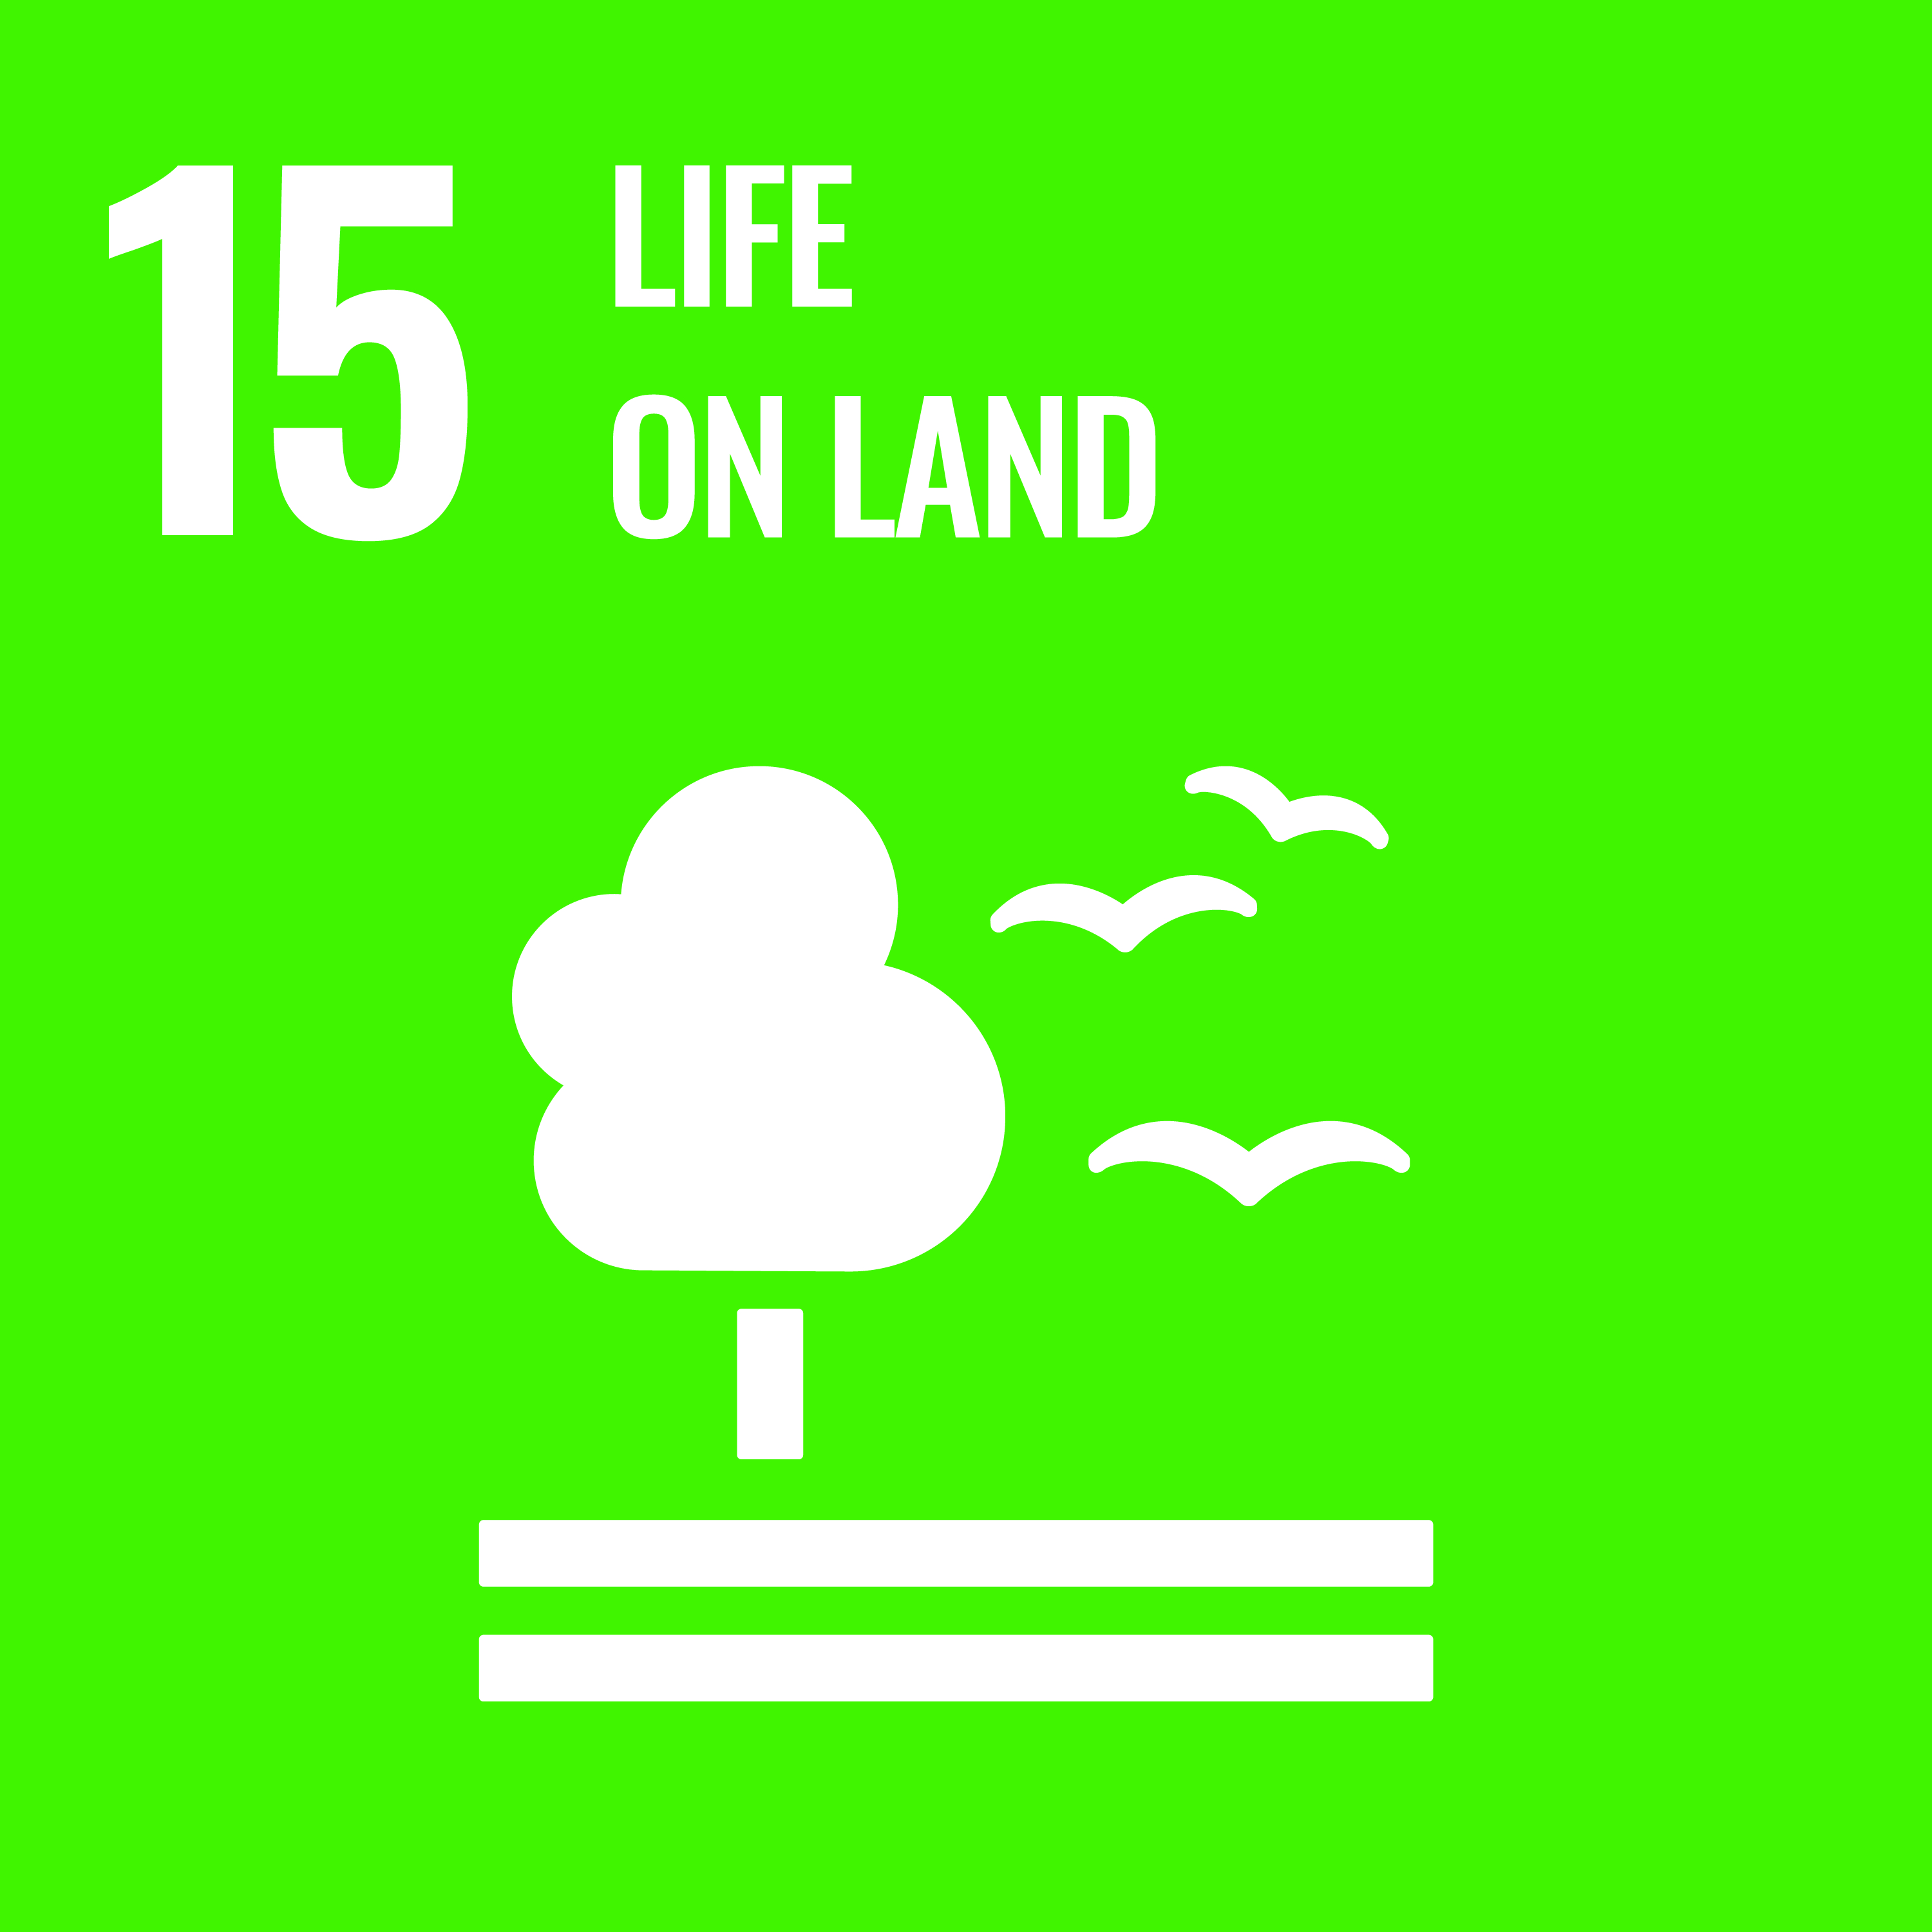
\includegraphics[width=\linewidth]{Pictures/ODD/ODD15.jpg}
	\end{minipage}
	\hfill
	\begin{minipage}{0.8\textwidth}
		{\bfseries\Large ODD 15 : }\\[2pt]
		\textit{Préserver et restaurer les écosystèmes terrestres, gérer durablement les forêts, lutter contre la désertification, enrayer et inverser la dégradation des terres et mettre fin à l’appauvrissement de la biodiversité.}
	\end{minipage}
\end{simplebox2}




\section{ODD 15 : Vie terrestre}

\subsection{Cible 15.1 : Protection des écosystèmes terrestres et d’eau douce}

La cible 15.1 vise à assurer la conservation et la restauration des écosystèmes terrestres et d’eau douce, en protégeant les zones clés pour la biodiversité.

\begin{figure}[H]
	\centering
	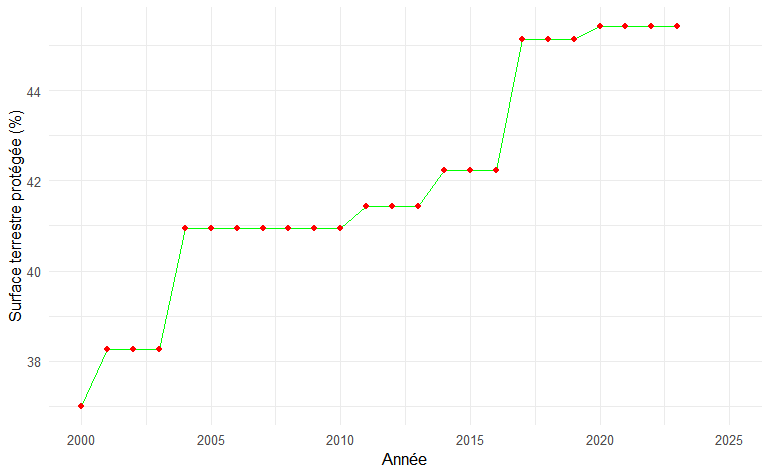
\includegraphics[width=0.75\textwidth]{Pictures/graphs/sdg15_cpta.png}
	\caption{Évolution de la surface protégée dans les sites terrestres importants pour la biodiversité}
	\label{fig:sdg15_cpta}
\end{figure}

La part des surfaces terrestres protégées a progressivement augmenté de 37\% à 45\%, ce qui montre un effort continu du Sénégal pour préserver les habitats terrestres essentiels. Bien que cette tendance soit positive, l’objectif d’une protection complète reste encore loin.

\begin{figure}[H]
	\centering
	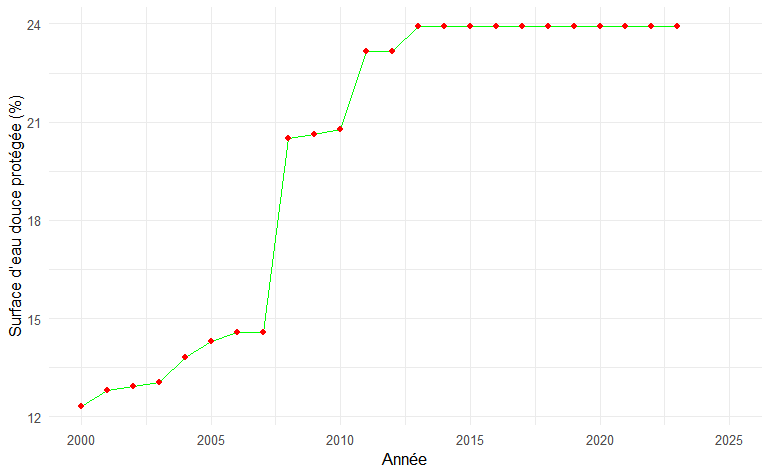
\includegraphics[width=0.75\textwidth]{Pictures/graphs/sdg15_cpfa.png}
	\caption{Évolution de la surface protégée dans les sites d’eau douce importants pour la biodiversité}
	\label{fig:sgd15_cpfa}
\end{figure}

Les sites d’eau douce protégés ont connu une augmentation significative, passant de 12\% à 24\%, traduisant la prise en compte progressive des écosystèmes aquatiques intérieurs dans les politiques de conservation.



\section*{Synthèse de la performance - ODD15}

\begin{figure}[H]
	\centering
	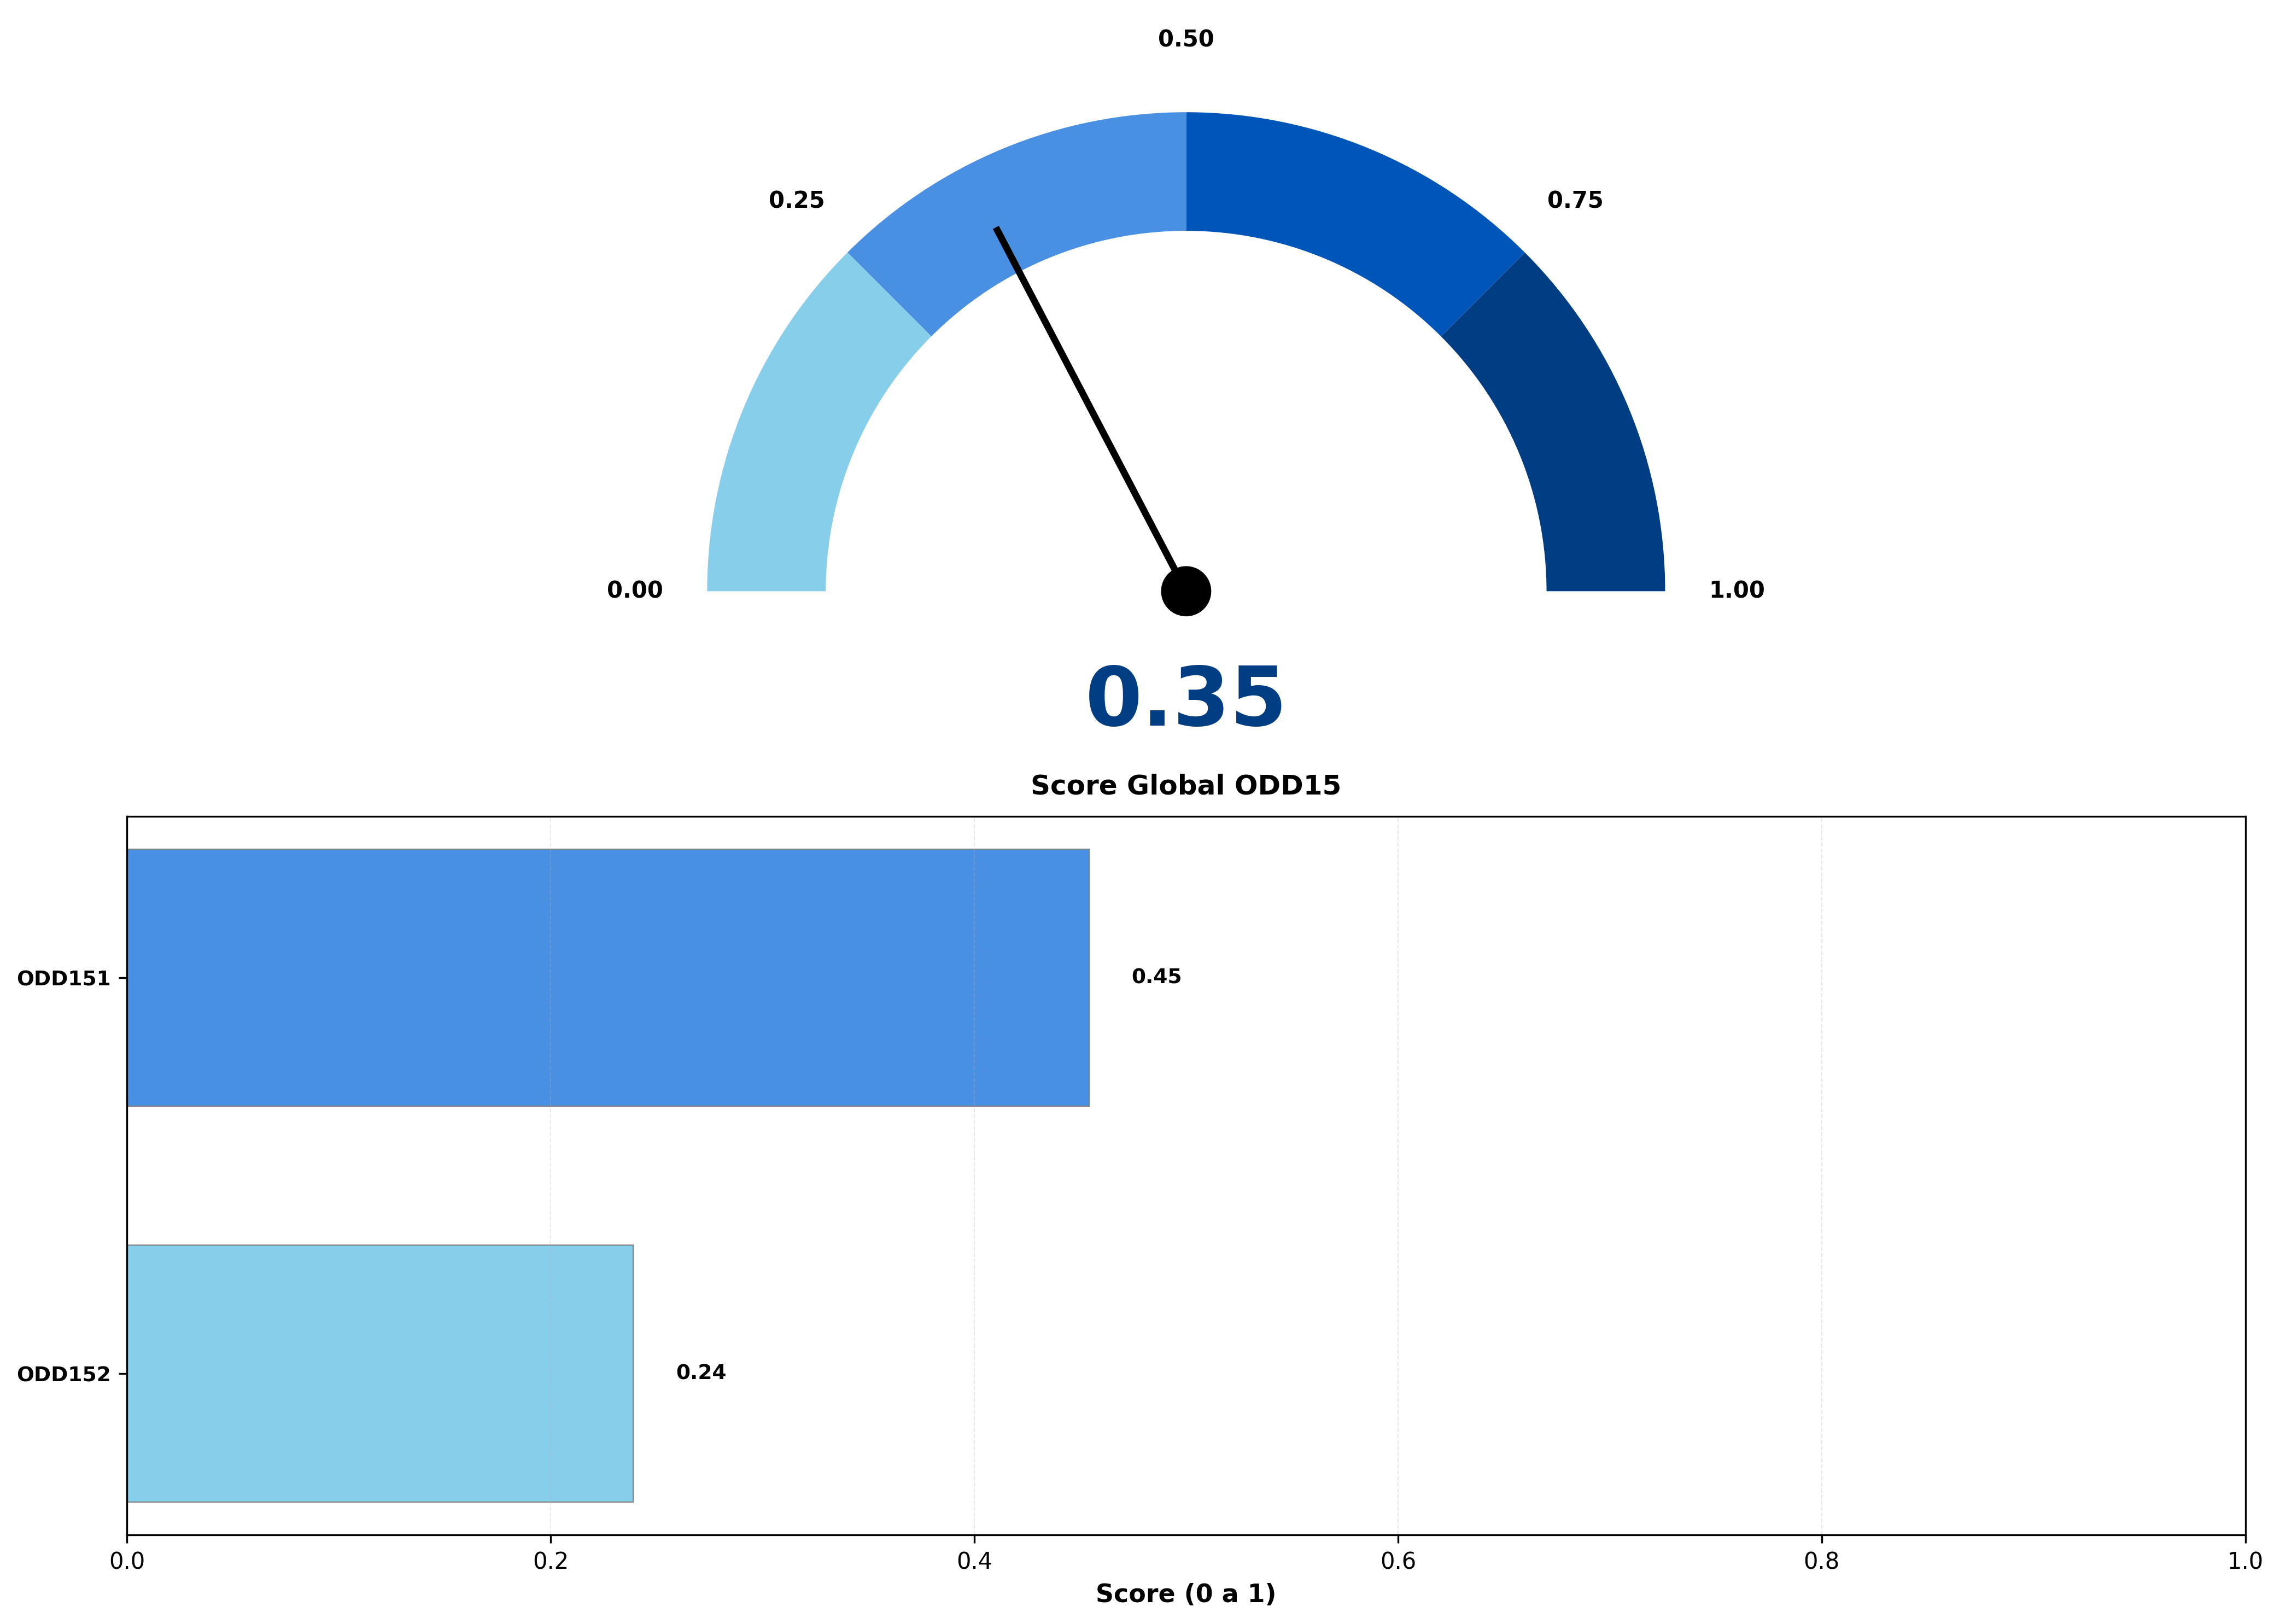
\includegraphics[width=0.95\textwidth]{Pictures/graphs/ODD15_scores.png}
	\caption{Performance par indicateur - ODD15}
\end{figure}
s
\begin{table}[H]
	\centering
	\begin{tabularx}{\textwidth}{l l c c c}
		\rowcolor[HTML]{003D82}
		\color{white}\textbf{Code} & \color{white}\textbf{Indicateur} & \color{white}\textbf{Valeur} & \color{white}\textbf{Cible} & \color{white}\textbf{Score} \\
		\rowcolor[HTML]{F5F8FC}
		ODD151 & \% de surface protégée en eau douce & 23.91 & 100.00 & 0.24 \\
		\rowcolor[HTML]{E8F0FF}
		ODD152 & \% de surface protégée terrestre & 45.41 & 100.00 & 0.45 \\
	\end{tabularx}
\end{table}

L'analyse du ODD15 révèle un score global de 0.3466, basé sur 2 indicateur(s). Les performances varient de 0.24 à 0.45, montrant une certaine disparité dans la mise en oeuvre des cibles. Les indicateurs critiques (score < 0,30) nécessitent une attention particulière.



%%%%%%%%%%%%%%%%%%%%% ODD16 %%%%%%%%%%%%%%%%%%%%%%%%%%%

\newpage
\begin{simplebox2}
	
	\begin{minipage}{0.15\textwidth}
		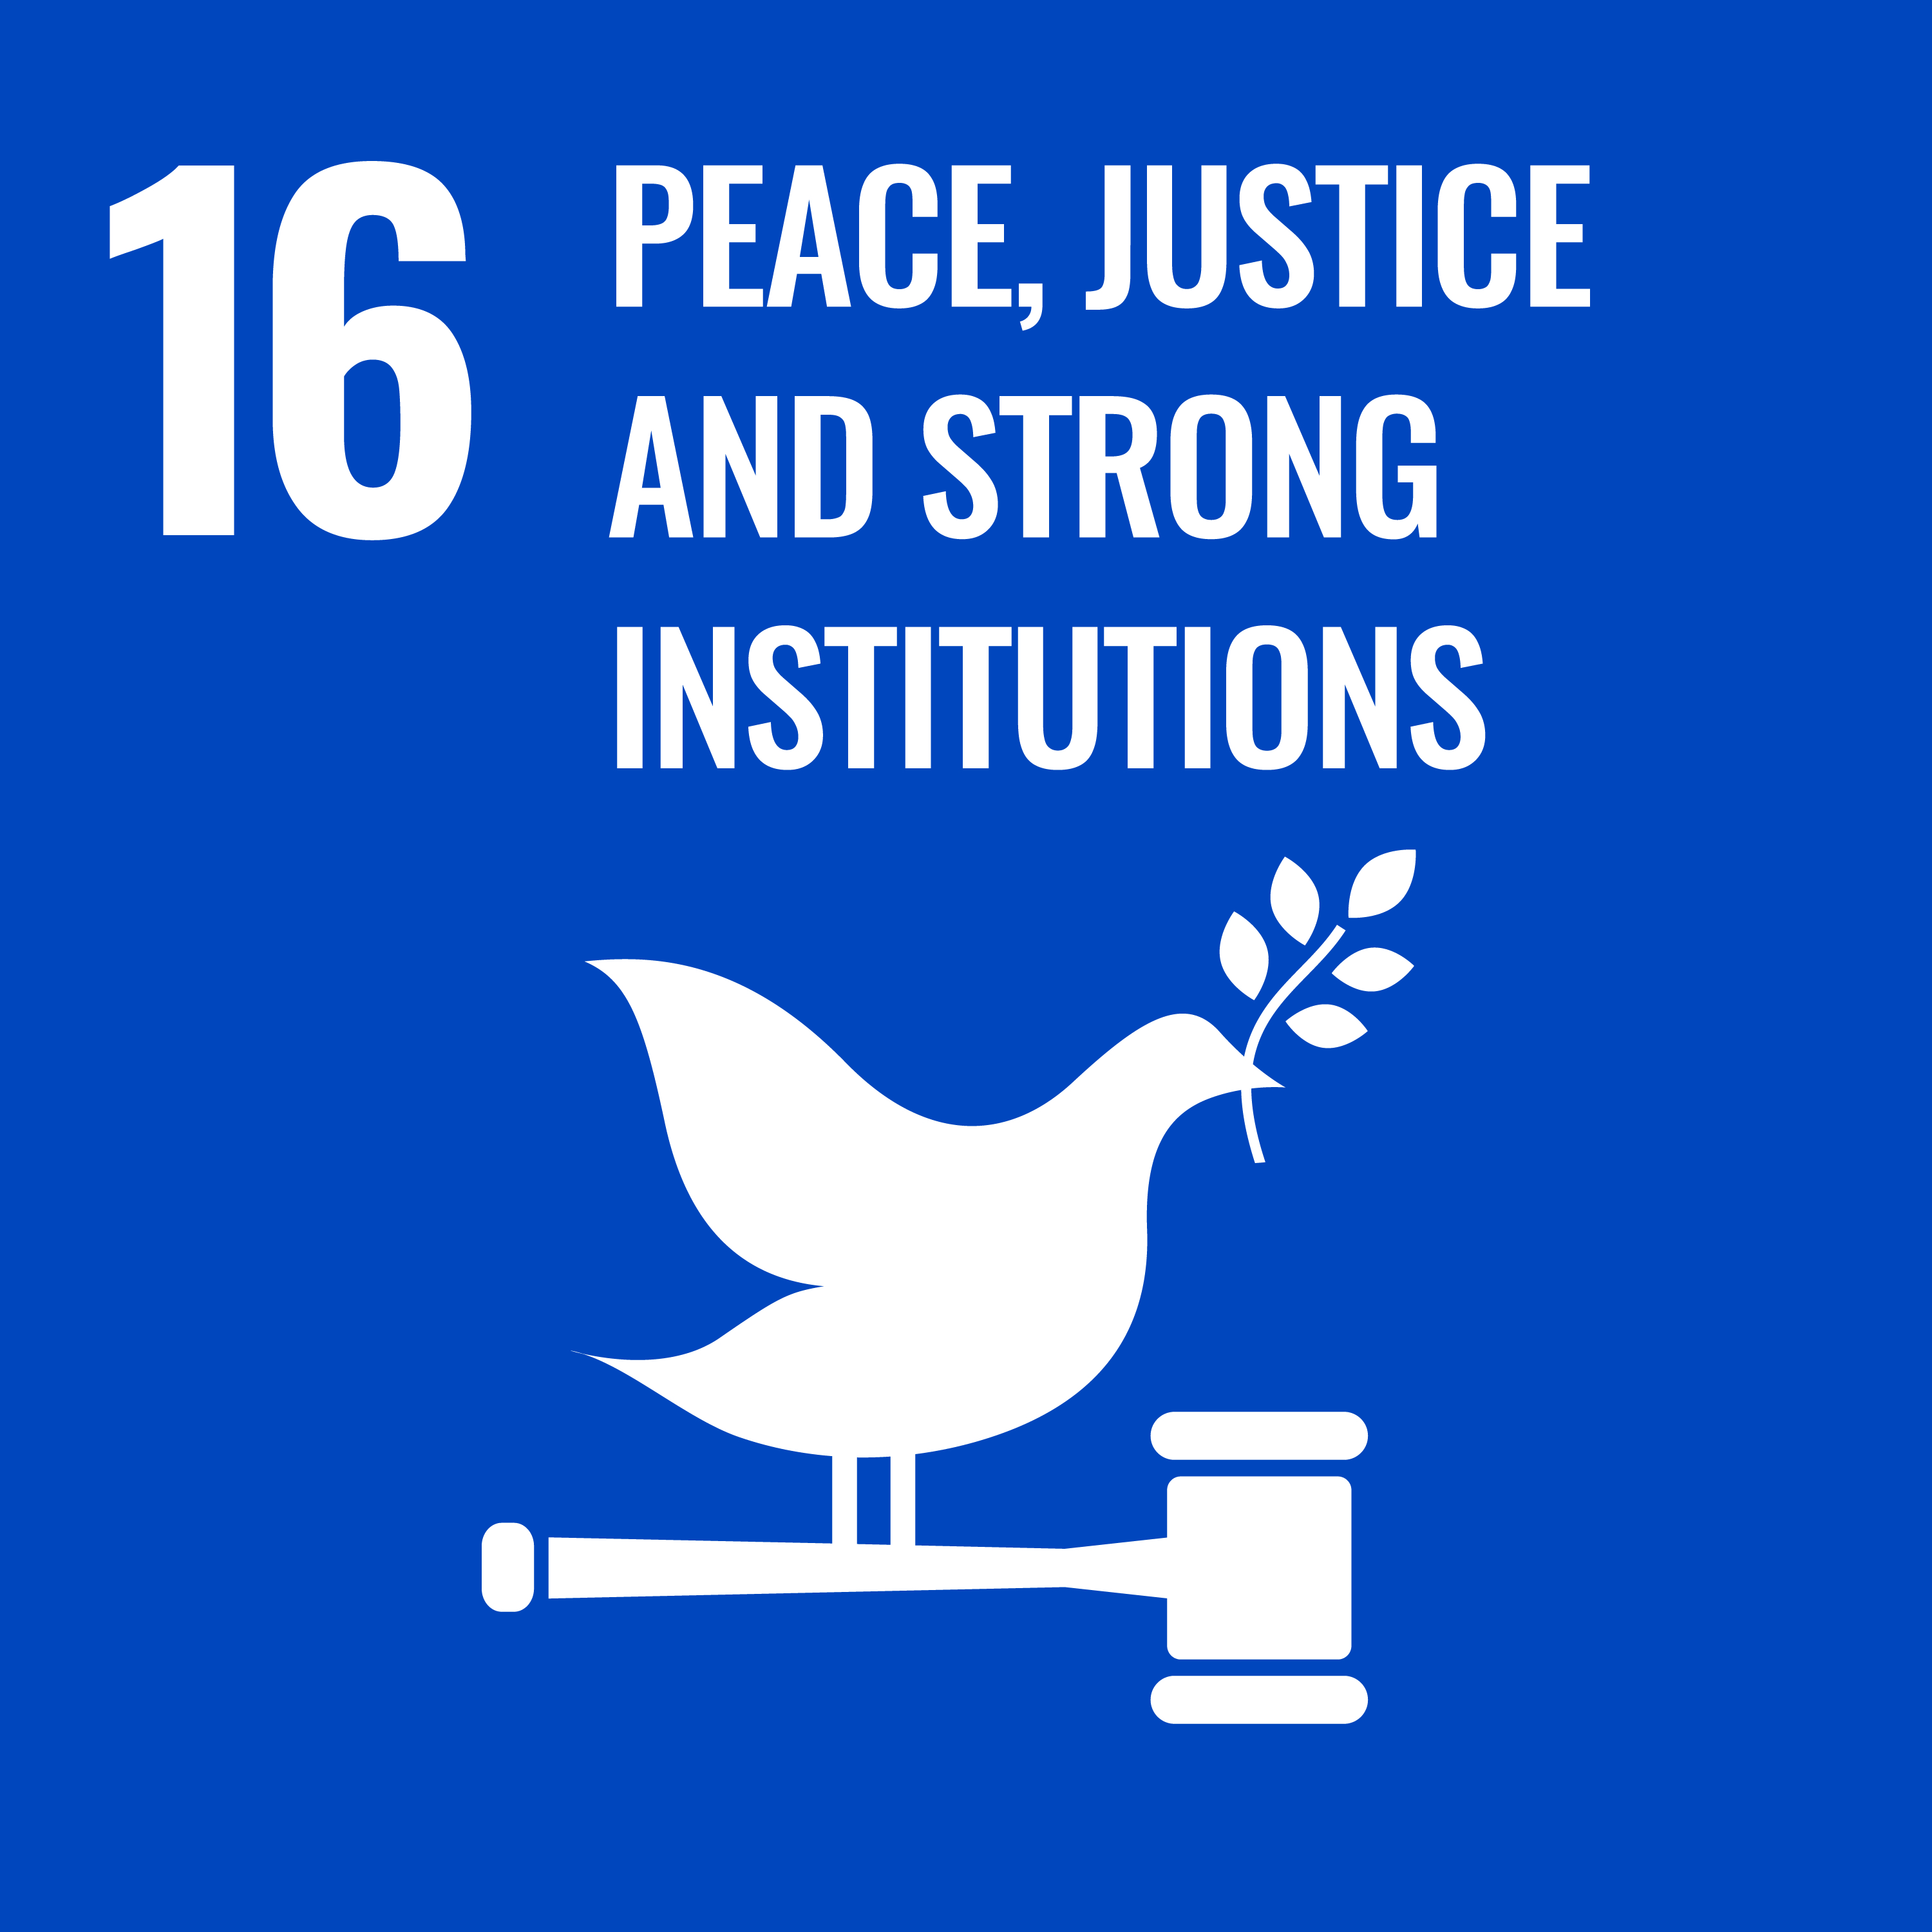
\includegraphics[width=\linewidth]{Pictures/ODD/ODD16.jpg}
	\end{minipage}
	\hfill
	\begin{minipage}{0.8\textwidth}
		{\bfseries\Large ODD 16 : }\\[2pt]
		\textit{Promouvoir l’avènement de sociétés pacifiques et inclusives aux fins du développement durable, assurer l’accès de tous à la justice et mettre en place, à tous les niveaux, des institutions efficaces, responsables et ouvertes.}
	\end{minipage}
\end{simplebox2}



\section{ODD 16 : Paix, justice et institutions efficaces}

L'ODD 16 vise à promouvoir des sociétés pacifiques et inclusives, à garantir l'accès à la justice pour tous et à mettre en place des institutions efficaces, responsables et transparentes. Les données disponibles pour le Sénégal permettent de suivre plusieurs dimensions de cet objectif, notamment la sécurité, l'accès à la justice, la liberté de la presse et la corruption. 

Les indicateurs relatifs à la sécurité montrent que l'indice de sécurité est passé de 0,74 à 0,67 au fil des années disponibles, indiquant une stabilité relative avec une légère baisse sur certaines périodes. L'enregistrement des naissances des enfants de moins de cinq ans fluctue entre 36\% et 45\%, montrant un progrès modéré mais encore insuffisant pour assurer une couverture complète. Le Corruption Perceptions Index varie de 55,44 à 76,01 sur la période, traduisant des améliorations ponctuelles mais également des disparités persistantes dans la perception de la corruption. La liberté de la presse, mesurée par l'indice correspondant, varie entre 61,49 et 80,26, témoignant d'une ouverture progressive des médias et d'un environnement plus transparent. L'accès à la justice et la rapidité des procédures administratives sont respectivement autour de 0,63-0,74 et 0,55-0,74 sur l'échelle 0-1, ce qui montre des progrès significatifs mais laisse apparaître des marges d'amélioration.  

En combinant ces chiffres, on constate que le Sénégal a réalisé certains progrès dans le renforcement de la sécurité et des institutions, avec des indicateurs relativement stables et quelques améliorations notables. Cependant, la persistance de défis tels que la perception de la corruption et le taux de naissance non enregistré montre que des efforts restent nécessaires pour atteindre pleinement les cibles de l'ODD 16. Les données indiquent donc qu'il est crucial de poursuivre le renforcement des institutions, d'améliorer la gouvernance et d'assurer une justice accessible et efficace pour l'ensemble de la population.


\section*{Synthèse de la performance - ODD16}

\begin{figure}[H]
	\centering
	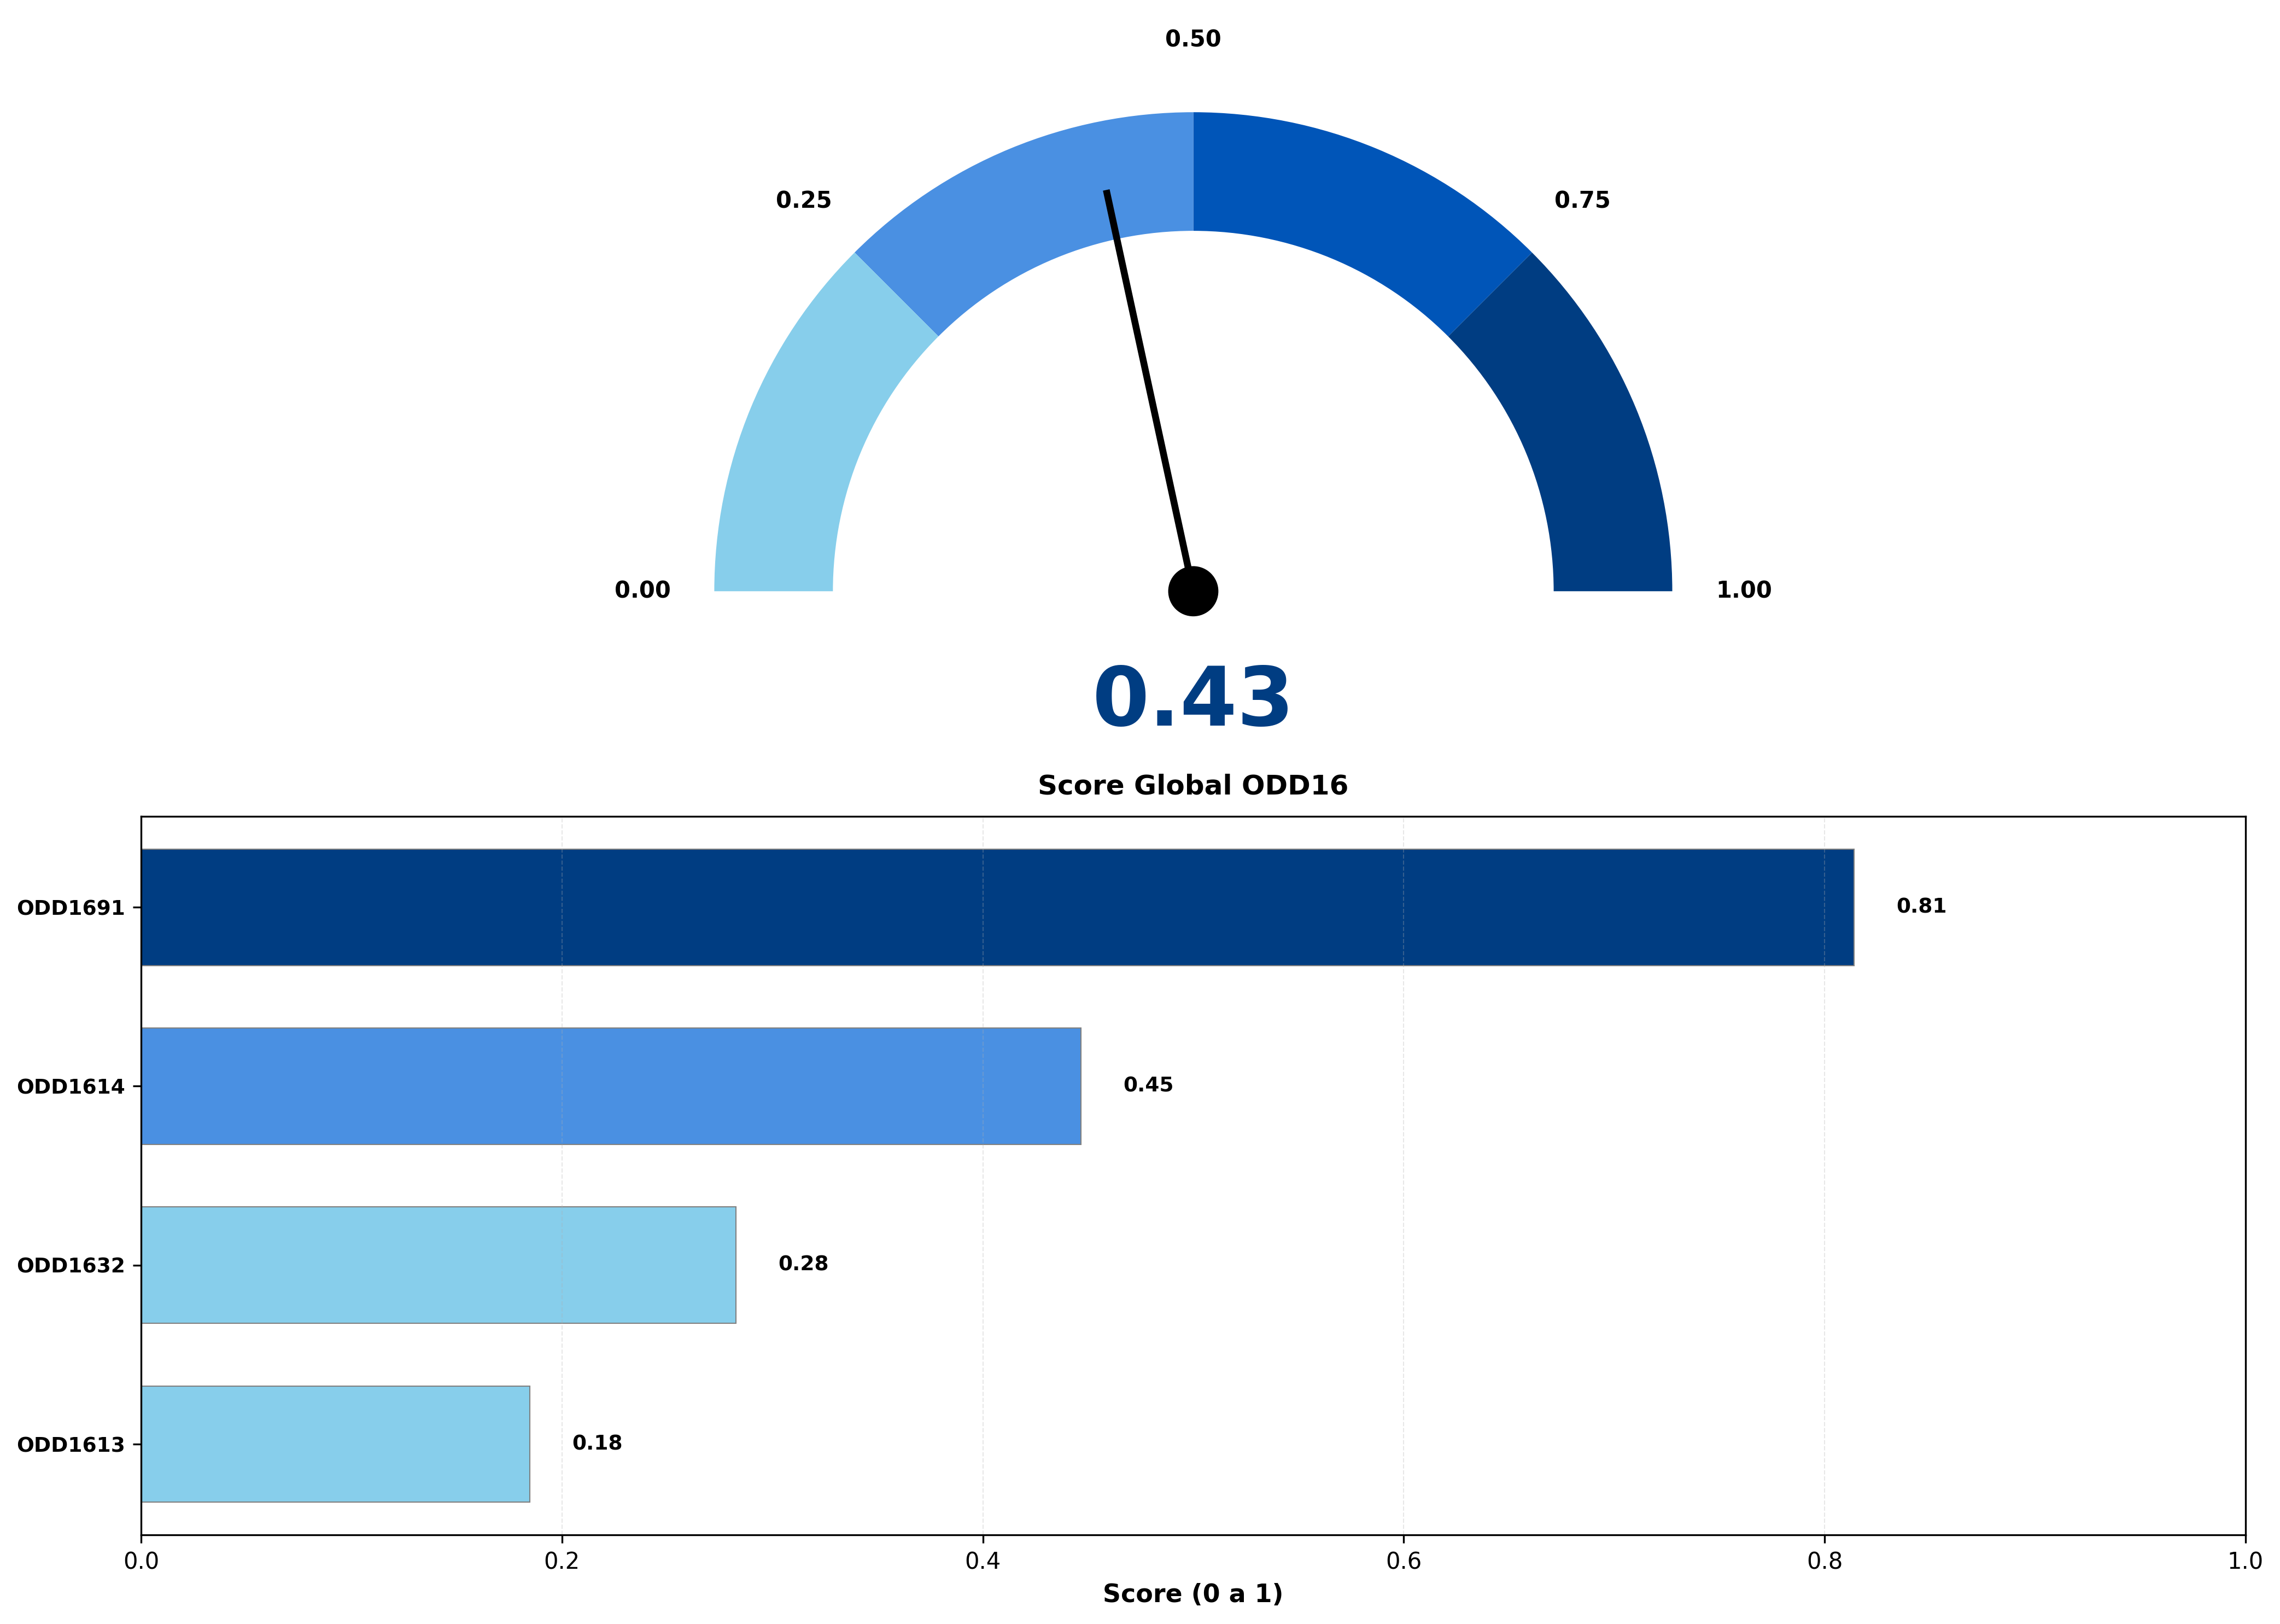
\includegraphics[width=0.95\textwidth]{Pictures/graphs/ODD16_scores.png}
	\caption{Performance par indicateur - ODD16}
\end{figure}

\begin{table}[H]
	\centering
	\begin{tabularx}{\textwidth}{l l c c c}
		\rowcolor[HTML]{003D82}
		\color{white}\textbf{Code} & \color{white}\textbf{Indicateur} & \color{white}\textbf{Valeur} & \color{white}\textbf{Cible} & \color{white}\textbf{Score} \\
		\rowcolor[HTML]{F5F8FC}
		ODD1613 & Victimes de violences physiques, psychologiques ou sexuelles & 0.32 & 0.05 & 0.18 \\
		\rowcolor[HTML]{E8F0FF}
		ODD1632 & Population carcérale en instance de jugement & 0.54 & 0.00 & 0.28 \\
		\rowcolor[HTML]{F5F8FC}
		ODD1614 & Proportion considérant sans risque le fait de marcher seul & 0.34 & 0.75 & 0.45 \\
		\rowcolor[HTML]{E8F0FF}
		ODD1691 & Enregistrement à l'Etat civil & 0.81 & 1.00 & 0.81 \\
	\end{tabularx}
\end{table}

L'analyse du ODD16 révèle un score global de 0.4320, basé sur 4 indicateur(s). Les performances varient de 0.18 à 0.81, montrant une certaine disparité dans la mise en oeuvre des cibles. Les indicateurs critiques (score < 0,30) nécessitent une attention particulière.





%%%%%%%%%%%%%%%%%%%%% ODD17 %%%%%%%%%%%%%%%%%%%%%%%%%%%

\newpage
\begin{simplebox2}
	
	\begin{minipage}{0.15\textwidth}
		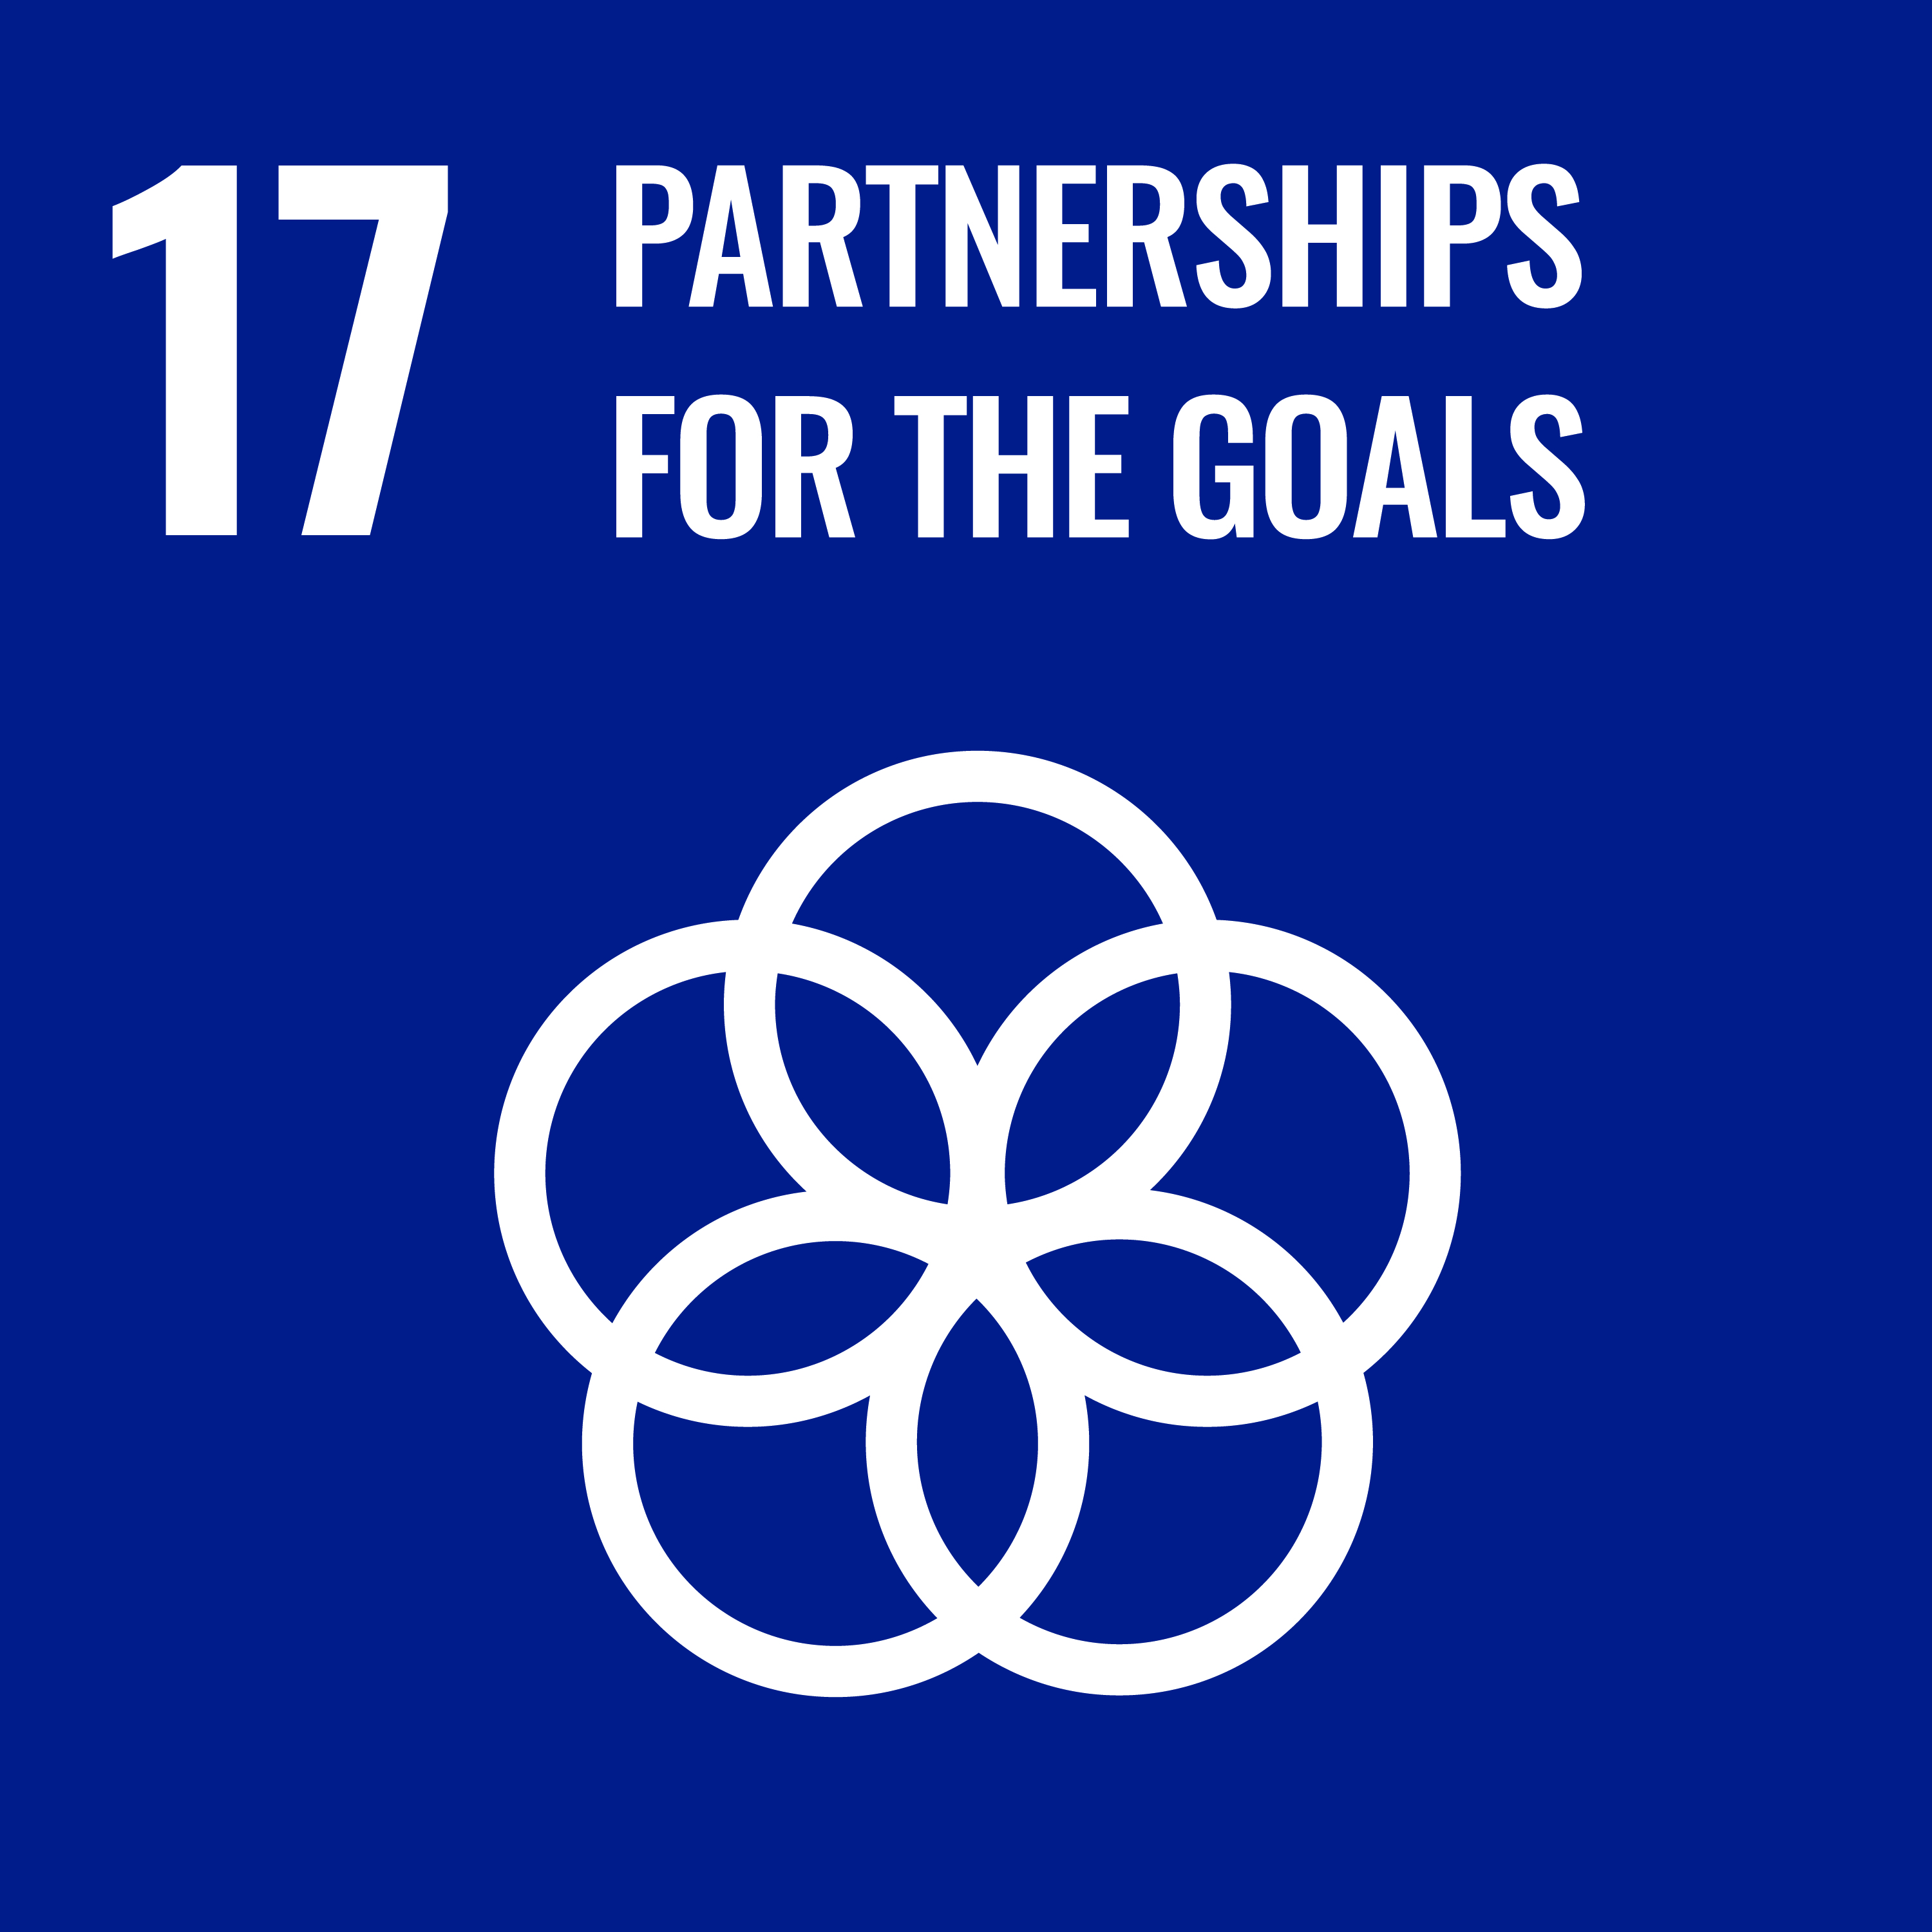
\includegraphics[width=\linewidth]{Pictures/ODD/ODD17.jpg}
	\end{minipage}
	\hfill
	\begin{minipage}{0.8\textwidth}
		{\bfseries\Large ODD 17 : }\\[2pt]
		\textit{Renforcer les moyens de mettre en œuvre le Partenariat mondial pour le développement durable et le revitaliser.}
	\end{minipage}
\end{simplebox2}



\section{ODD 17 : Partenariats pour la réalisation des objectifs}

La cible 17.9 vise à « accroître l’aide publique au développement pour les pays en développement et mobiliser des ressources financières internes, y compris à travers une amélioration de la mobilisation des recettes publiques, pour renforcer la capacité nationale à mettre en œuvre des programmes de santé et d’éducation ». L’indicateur utilisé ici est la part du PIB consacrée par le gouvernement à la santé et à l’éducation, reflétant directement la capacité nationale à financer ces secteurs essentiels.

\begin{figure}[H]
	\centering
	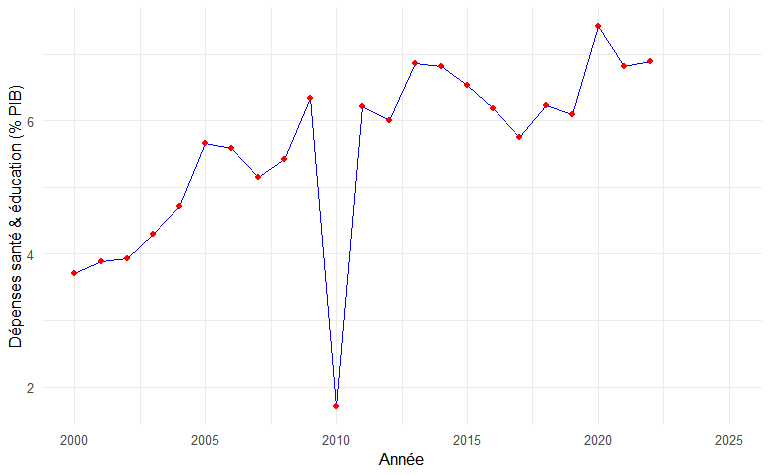
\includegraphics[width=0.8\textwidth]{Pictures/graphs/sdg17_govex.png}
	\caption{Évolution de la part du PIB consacrée à la santé et à l'éducation au Sénégal (ODD 17, cible 17.9)}
\end{figure}

L’analyse des données montre une progression globale de cet indicateur, passant de 3,71\% à 7,41\% du PIB sur la période considérée. Cette tendance traduit un engagement croissant du gouvernement dans le financement des secteurs sociaux stratégiques, essentiels à l’amélioration de la santé, de l’éducation et à la réduction des inégalités. 

Cependant, certaines fluctuations ponctuelles, notamment la baisse à 1,71\% observée à une période donnée, mettent en évidence des contraintes budgétaires temporaires ou des ajustements économiques. Cela souligne l’importance de maintenir un financement stable et soutenu pour garantir la continuité des programmes sociaux. 

En conclusion, le Sénégal montre des progrès significatifs pour renforcer sa capacité nationale à soutenir les ODD à travers des investissements publics dans la santé et l’éducation, conformément à la cible 17.9. La continuité et la stabilité de ces dépenses restent toutefois cruciales pour atteindre pleinement les objectifs fixés.

\section*{Synthèse de la performance - ODD17}

\begin{figure}[H]
	\centering
	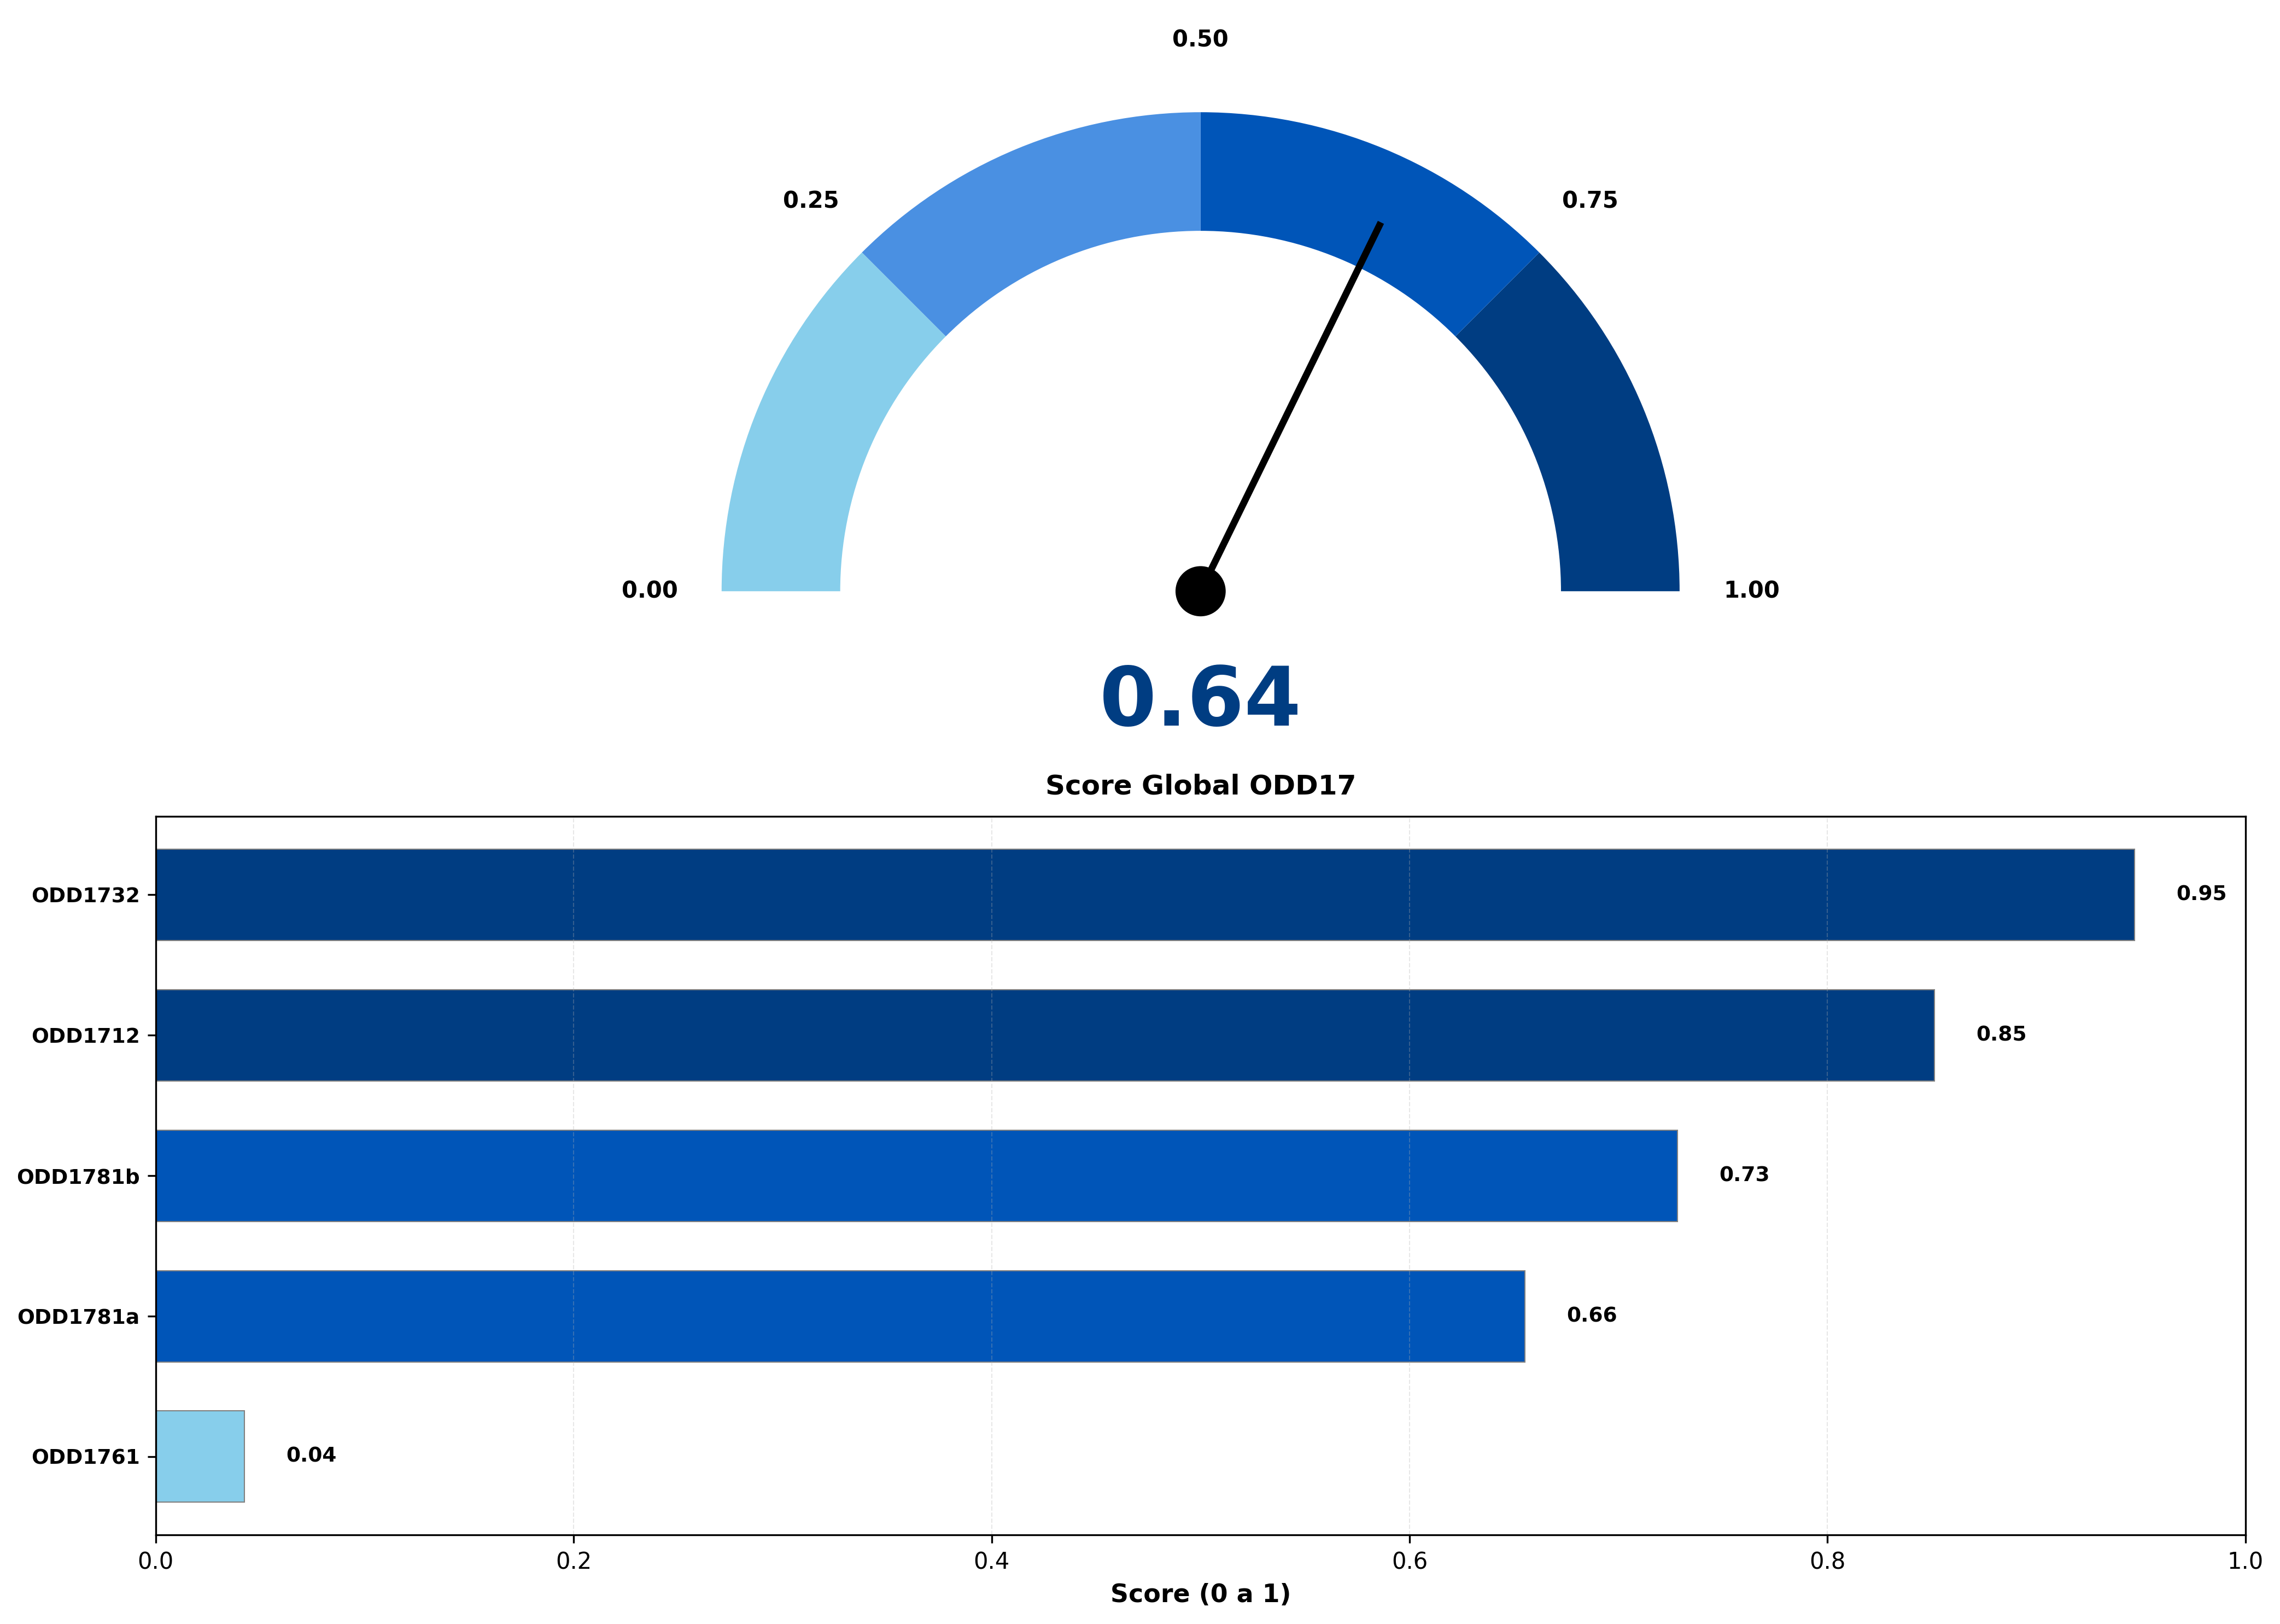
\includegraphics[width=0.95\textwidth]{Pictures/graphs/ODD17_scores.png}
	\caption{Performance par indicateur - ODD17}
\end{figure}

\begin{table}[H]
	\centering
	\begin{tabularx}{\textwidth}{l l c c c}
		\rowcolor[HTML]{003D82}
		\color{white}\textbf{Code} & \color{white}\textbf{Indicateur} & \color{white}\textbf{Valeur} & \color{white}\textbf{Cible} & \color{white}\textbf{Score} \\
		\rowcolor[HTML]{F5F8FC}
		ODD1761 & Abonnements à une connexion Internet à haut débit fixe & 0.64 & 15.00 & 0.04 \\
		\rowcolor[HTML]{E8F0FF}
		ODD1781a & Utilisation de l'internet (Femmes) & 0.66 & 1.00 & 0.66 \\
		\rowcolor[HTML]{F5F8FC}
		ODD1781b & Utilisation de l'internet (Homme) & 0.73 & 1.00 & 0.73 \\
		\rowcolor[HTML]{E8F0FF}
		ODD1712 & Budget national financé par les impôts nationaux  & 0.85 & 1.00 & 0.85 \\
		\rowcolor[HTML]{F5F8FC}
		ODD1732 & Envois de fonds des travailleurs migrants & 0.09 & 0.10 & 0.95 \\
	\end{tabularx}
\end{table}

L'analyse du ODD17 révèle un score global de 0.6447, basé sur 5 indicateur(s). Les performances varient de 0.04 à 0.95, montrant une certaine disparité dans la mise en oeuvre des cibles. Les indicateurs critiques (score < 0,30) nécessitent une attention particulière.

